%%%%%%%%%%%%%%%%%%%%%%%%%%%%%%%%%%%%%%%%%
% Masters/Doctoral Thesis 
% LaTeX Template
% Version 2.5 (27/8/17)
%
% This template was downloaded from:
% http://www.LaTeXTemplates.com
%
% Version 2.x major modifications by:
% Vel (vel@latextemplates.com)
%
% This template is based on a template by:
% Steve Gunn (http://users.ecs.soton.ac.uk/srg/softwaretools/document/templates/)
% Sunil Patel (http://www.sunilpatel.co.uk/thesis-template/)
%
% Template license:
% CC BY-NC-SA 3.0 (http://creativecommons.org/licenses/by-nc-sa/3.0/)
%
%%%%%%%%%%%%%%%%%%%%%%%%%%%%%%%%%%%%%%%%%

%----------------------------------------------------------------------------------------
%	PACKAGES AND OTHER DOCUMENT CONFIGURATIONS
%----------------------------------------------------------------------------------------

\documentclass[
11pt, % The default document font size, options: 10pt, 11pt, 12pt
%oneside, % Two side (alternating margins) for binding by default, uncomment to switch to one side
english,
french,% ngerman for German
singlespacing, % Single line spacing, alternatives: onehalfspacing or doublespacing
%draft, % Uncomment to enable draft mode (no pictures, no links, overfull hboxes indicated)
%nolistspacing, % If the document is onehalfspacing or doublespacing, uncomment this to set spacing in lists to single
%liststotoc, % Uncomment to add the list of figures/tables/etc to the table of contents
%toctotoc, % Uncomment to add the main table of contents to the table of contents
%parskip, % Uncomment to add space between paragraphs
%nohyperref, % Uncomment to not load the hyperref package
headsepline, % Uncomment to get a line under the header
chapterinoneline, % Uncomment to place the chapter title next to the number on one line
%consistentlayout, % Uncomment to change the layout of the declaration, abstract and acknowledgements pages to match the default layout
]{MastersDoctoralThesis} % The class file specifying the document structure

% \usepackage[french]{babel}

\usepackage[utf8]{inputenc} % Required for inputting international characters
\usepackage[T1]{fontenc} % Output font encoding for international characters

\usepackage{mathpazo} % Use the Palatino font by default

\usepackage[backend=biber,style=ieee,natbib=true]{biblatex} % Use the bibtex backend with the authoryear citation style (which resembles APA)

\addbibresource{myreferences.bib} % The filename of the bibliography

\usepackage[autostyle=true]{csquotes} % Required to generate language-dependent quotes in the bibliography

\usepackage[utf8]{inputenc}
% \usepackage{acronym}
\usepackage[acronym, toc]{glossaries}
\makeglossaries

\usepackage{placeins}
\usepackage{listings}
\usepackage{multirow}
\usepackage{hhline}

%----------------------------------------------------------------------------------------
%	MARGIN SETTINGS
%----------------------------------------------------------------------------------------

\geometry{
	paper=a4paper, % Change to letterpaper for US letter
	inner=2.5cm, % Inner margin
	outer=3.8cm, % Outer margin
	bindingoffset=.5cm, % Binding offset
	top=1.5cm, % Top margin
	bottom=1.5cm, % Bottom margin
	%showframe, % Uncomment to show how the type block is set on the page
}

%----------------------------------------------------------------------------------------
%	THESIS INFORMATION
%----------------------------------------------------------------------------------------

\thesistitle{Détection rapide de jets basée sur l'apprentissage automatique pour le traitement en temps réel sur FPGA au sein de l'expérience ATLAS au LHC} % Your thesis title, this is used in the title and abstract, print it elsewhere with \ttitle
\supervisor{Prof. Alexandros \textsc{Kalousis} \\
Prof. Andres \textsc{Upegui} \\
Prof. Anna \textsc{Sfyrla}} % Your supervisor's name, this is used in the title page, print it elsewhere with \supname
\examiner{} % Your examiner's name, this is not currently used anywhere in the template, print it elsewhere with \examname
\degree{Master en Sciences Informatiques} % Your degree name, this is used in the title page and abstract, print it elsewhere with \degreename
\author{David \textsc{Nogueiras Blanco}} % Your name, this is used in the title page and abstract, print it elsewhere with \authorname
\addresses{} % Your address, this is not currently used anywhere in the template, print it elsewhere with \addressname

\subject{Sciences Informatiques} % Your subject area, this is not currently used anywhere in the template, print it elsewhere with \subjectname
\keywords{} % Keywords for your thesis, this is not currently used anywhere in the template, print it elsewhere with \keywordnames
\university{{Université de Genève}} % Your university's name and URL, this is used in the title page and abstract, print it elsewhere with \univname
\department{{Département d'informatique}} % Your department's name and URL, this is used in the title page and abstract, print it elsewhere with \deptname
% \group{\href{http://researchgroup.university.com}{Research Group Name}} % Your research group's name and URL, this is used in the title page, print it elsewhere with \groupname
\faculty{{Faculté des Sciences}} % Your faculty's name and URL, this is used in the title page and abstract, print it elsewhere with \facname

\AtBeginDocument{
\hypersetup{pdftitle=\ttitle} % Set the PDF's title to your title
\hypersetup{pdfauthor=\authorname} % Set the PDF's author to your name
\hypersetup{pdfkeywords=\keywordnames} % Set the PDF's keywords to your keywords
}

\begin{document}

\frontmatter % Use roman page numbering style (i, ii, iii, iv...) for the pre-content pages

\pagestyle{plain} % Default to the plain heading style until the thesis style is called for the body content

%----------------------------------------------------------------------------------------
%	TITLE PAGE
%----------------------------------------------------------------------------------------

\begin{titlepage}
\begin{center}

\vspace*{.06\textheight}
{\scshape\LARGE \univname\par}\vspace{1.5cm} % University name
\textsc{\Large Mémoire de Maîtrise en Sciences Informatiques}\\[0.5cm] % Thesis type

\HRule \\[0.4cm] % Horizontal line
{\huge \bfseries \ttitle\par}\vspace{0.4cm} % Thesis title
\HRule \\[1.5cm] % Horizontal line
 
\begin{minipage}[t]{0.4\textwidth}
\begin{flushleft} \large
\emph{Auteur :}\\
{\authorname} % Author name - remove the \href bracket to remove the link
\end{flushleft}
\end{minipage}
\begin{minipage}[t]{0.4\textwidth}
\begin{flushright} \large
\emph{Superviseurs :} \\
{\supname} % Supervisor name - remove the \href bracket to remove the link  
\end{flushright}
\end{minipage}\\[2cm]
 
\vfill

\large \textit{Un travail soumis dans le cadre du \\ \degreename}\\ % University requirement text
\textit{}\\
\facname\\\deptname\\[1cm]

\includegraphics[scale=0.5]{Figures/unige_sciences.png}

\vfill

{\large \today}\\[4cm] % Date

 
\vfill
\end{center}
\end{titlepage}

%----------------------------------------------------------------------------------------
%	DECLARATION PAGE
%----------------------------------------------------------------------------------------

% \begin{declaration}
% \addchaptertocentry{\authorshipname} % Add the declaration to the table of contents
% \noindent I, \authorname, declare that this thesis titled, \enquote{\ttitle} and the work presented in it are my own. I confirm that:

% \begin{itemize} 
% \item This work was done wholly or mainly while in candidature for a research degree at this University.
% \item Where any part of this thesis has previously been submitted for a degree or any other qualification at this University or any other institution, this has been clearly stated.
% \item Where I have consulted the published work of others, this is always clearly attributed.
% \item Where I have quoted from the work of others, the source is always given. With the exception of such quotations, this thesis is entirely my own work.
% \item I have acknowledged all main sources of help.
% \item Where the thesis is based on work done by myself jointly with others, I have made clear exactly what was done by others and what I have contributed myself.\\
% \end{itemize}
 
% \noindent Signed:\\
% \rule[0.5em]{25em}{0.5pt} % This prints a line for the signature
 
% \noindent Date:\\
% \rule[0.5em]{25em}{0.5pt} % This prints a line to write the date
% \end{declaration}

% \cleardoublepage

%----------------------------------------------------------------------------------------
%	QUOTATION PAGE
%----------------------------------------------------------------------------------------

% \vspace*{0.2\textheight}

% \noindent\enquote{\itshape Thanks to my solid academic training, today I can write hundreds of words on virtually any topic without possessing a shred of information, which is how I got a good job in journalism.}\bigbreak

% \hfill Dave Barry

%----------------------------------------------------------------------------------------
%	ABSTRACT PAGE
%----------------------------------------------------------------------------------------

\begin{abstract}
\addchaptertocentry{\abstractname} % Add the abstract to the table of contents

Dans le cadre de l'expérience \acrfull{atlas} au sein du \acrfull{lhc} au \acrfull{cern}, des particules entrent en collision toutes les $25 ns$ générant environ $25$ MB de données. De par la fréquence élevée de ces événements et la quantité de données en résultant, il est indispensable de conserver uniquement les interactions intéressantes. Afin d'effectuer cette sélection en temps réel, un système de déclenchement à deux niveaux a été mis en place. Le premier est caractérisé par une très faible latence, de moins de 2.5 ms, implémenté sur de l'électronique dédiée et sur des \acrfull{fpga}. Le second effectue des analyses détaillées de chaque collision dans de grandes fermes de processeurs. La fréquence initiale de 40 MHz peut ainsi être diminuée à 100 kHz puis à 1 kHz. Parmi les données traitées, celles contenant des jets sont utilisées s'ils sont présents en grand nombre, ou s'ils sont très énergétiques. Ceux-ci résultent de processus complexes, et sont habituellement observés suite à une collision entre protons.

Le but de ce travail de master est de développer un algorithme d'apprentissage automatique pour la reconstruction de jets en temps réel sur \acrshort{fpga}. Pour ce faire, le modèle YOLOv8, étant à la pointe pour les tâches de vision par ordinateur, est utilisé et évalué dans un premier temps, puis une version modifiée du réseau de neurones ResNet18 capable de réaliser de la détection, choisi pour son architecture relativement simple, est développé et évalué en Keras, quantifié avec QKeras, puis finalement synthétisé sur \acrshort{fpga} à l'aide de l'outil \acrfull{hls4ml}. L'ensemble du projet contribue dans la recherche d'algorithmes de détection de jets en temps réel et de leur implémentation sous-jacente dans des systèmes à faible latence, en proposant l'évaluation à différents niveaux de deux réseaux neuronaux convolutifs pour cette tâche. 

Ce travail a mené à trois contributions ; le processus de développement complet de ResNet18+Tête pour une implémentation sur \acrshort{fpga}, la représentation de données complexes sous forme d'images, et la réalisation d'une procédure pour utiliser efficacement \acrshort{hls4ml}.

% Par ailleurs, la méthode de création d'images à partir de l'ensemble des données du calorimètre est documentée et disponible, ainsi qu'un logigramme de développement pour synthétiser un modèle avec \acrshort{hls4ml}.

\end{abstract}

%----------------------------------------------------------------------------------------
%	ACKNOWLEDGEMENTS
%----------------------------------------------------------------------------------------

\begin{acknowledgements}
\addchaptertocentry{\acknowledgementname} % Add the acknowledgements to the table of contents

Je souhaite remercier Monsieur Andres Upegui, Monsieur Alexandros Kalousis, et Madame Anna Sfyrla d'avoir rendu ce projet possible, ainsi que Madame Claire Antel, et Monsieur Leon Bozianu pour leur aide avec les jeux de données.

J'adresse un grand merci à ma famille, et mon entourage pour leur soutien indéfectible tout au long de ce travail et de mon master.

Finalement, je remercie également Madame Chloé Fouvy, et Monsieur Jean-Marc Boutay pour leur relecture et leur expertise, ainsi que Monsieur René Schneider et Monsieur Arnaud Gaudinat pour leur aide et la flexibilité qu'ils m'ont octroyés dans mon poste d'assistant HES.

\end{acknowledgements}

%----------------------------------------------------------------------------------------
%	LIST OF CONTENTS/FIGURES/TABLES PAGES
%----------------------------------------------------------------------------------------

\tableofcontents % Prints the main table of contents

% \listoffigures % Prints the list of figures
\cleardoublepage
\phantomsection
\renewcommand{\listfigurename}{Liste des figures}
\addcontentsline{toc}{chapter}{\listfigurename}
\listoffigures

% -----------------------------------------------------------------

% \listoftables % Prints the list of tables
\cleardoublepage
\phantomsection
\renewcommand{\listtablename}{Liste des tables}
\addcontentsline{toc}{chapter}{\listtablename}
\listoftables

%----------------------------------------------------------------------------------------
%	ABBREVIATIONS
%----------------------------------------------------------------------------------------

% \begin{abbreviations}{ll} % Include a list of abbreviations (a table of two columns)

% \textbf{ATLAS} & \textbf{A} \textbf{T}oroidal \textbf{L}HC \textbf{A}pparatu\textbf{S}\\
% \textbf{LHC} & \textbf{L}arge \textbf{H}adron \textbf{C}ollider\\
% \textbf{CERN} & \textbf{C}onseil \textbf{E}uropéen pour la \textbf{R}echerche \textbf{N}ucléaire\\
% \textbf{FPGA} & \textbf{F}ield \textbf{P}rogrammable \textbf{G}ate \textbf{A}rrays\\
% \textbf{CNN} & \textbf{C}onvolutionnal \textbf{N}eural \textbf{N}etwork\\

% \end{abbreviations}

%----------------------------------------------------------------------------------------
%	Acronyms
%----------------------------------------------------------------------------------------

%*******************************************************
% Acronyms
%*******************************************************
% \automark[section]{chapter}
% \renewcommand{\chaptermark}[1]{\markboth{\spacedlowsmallcaps{#1}}{\spacedlowsmallcaps{#1}}}
% \renewcommand{\sectionmark}[1]{\markright{\thesection\enspace\spacedlowsmallcaps{#1}}}
% \refstepcounter{dummy}
% \pdfbookmark[0]{Table des acronymes}{table des acronymes}
% \chapter*{Table des acronymes}

% Insert your acronyms here
% \begin{acronym}[UML]
%   \acro{DRY}{Don't Repeat Yourself}
%   \acro{API}{Application Programming Interface}
%   \acro{UML}{Unified Modeling Language}
% \end{acronym}

% \newglossaryentry{formula}
% {
%     name=formula,
%     description={A mathematical expression}
% }


\newacronym{atlas}{ATLAS}{A Toroidal LHC ApparatuS}
\newacronym{lhc}{LHC}{Large Hadron Collider}
\newacronym{cern}{CERN}{Conseil Européen pour la Recherche Nucléaire}
\newacronym{fpga}{FPGA}{Field Programmable Gate Arrays}
\newacronym{cnn}{CNN}{Convolutionnal Neural Network}
\newacronym{yolov8}{YOLOv8}{You Only Live Once version 8}
%-------------- State of the art ---------------------
\newacronym{hlt}{HLT}{High-Level Trigger}
\newacronym{cms}{CMS}{Compact Muon Solenoid}
\newacronym{jfex}{jFEX}{jet Feature Extractor}
\newacronym{asic}{ASIC}{Application-Specific Integrated Circuit}
\newacronym{cuda}{CUDA}{Compute Unified Device Architecture}
%-------------- ModelsUsed ---------------------
\newacronym{mlp}{MLP}{Multilayer Perceptron}
\newacronym{mse}{MSE}{Mean Squared Error}
\newacronym{relu}{ReLU}{Rectifier Linear Unit}
\newacronym{silu}{SiLU}{Sigmoid Linear Unit}
\newacronym{yolo}{YOLO}{You Only Look Once}
\newacronym{map}{mAP}{mean Average Precision}
\newacronym{cspnet}{CSPNet}{Cross Stage Partial Network}
\newacronym{spp}{SPP}{Spatial Pyramid Pooling}
\newacronym{sppf}{SPPF}{Spatial Pyramid Pooling Fast}
\newacronym{iou}{IoU}{Intersection over Union}
\newacronym{coco}{COCO}{Common Objects in Context}
%--------------------- Metrics ---------------------
\newacronym{ap}{AP}{Average Precision}
%--------------------- HLS4ML ---------------------
\newacronym{hls4ml}{HLS4ML}{High Level Synthesis for Machine Learning}
\newacronym{hls}{HLS}{High Level Synthesis}
\newacronym{rtl}{RTL}{Register Transfer Level}
%-------------- Results ---------------------
\newacronym{flops}{FLOPS}{Floating Point Operations Per Second}
\newacronym{dsp}{DSP}{Digital Signal Processor}
\newacronym{ff}{FF}{Flip-Flops}
\newacronym{lut}{LUT}{LookUp Table}
\newacronym{bram}{BRAM}{Digital Signal Processor}
\newacronym{fps}{FPS}{Frames Per Second}
\newacronym{ii}{II}{Initiation Interval}
\newacronym{cc}{CC}{clock cycles}

\glsenablehyper

% \printglossary[type=\acronymtype]
\printacronyms[title=Liste des acronymes, toctitle=Liste des acronymes]

\cleardoublepage
\renewcommand*{\glstextformat}[1]{\textcolor{darkgray}{#1}}

%----------------------------------------------------------------------------------------
%	PHYSICAL CONSTANTS/OTHER DEFINITIONS
%----------------------------------------------------------------------------------------

% \begin{constants}{lr@{${}={}$}l} % The list of physical constants is a three column table

% % The \SI{}{} command is provided by the siunitx package, see its documentation for instructions on how to use it

% % Speed of Light & $c_{0}$ & \SI{2.99792458e8}{\meter\per\second} (exact)\\
% %Constant Name & $Symbol$ & $Constant Value$ with units\\

% \end{constants}

%----------------------------------------------------------------------------------------
%	SYMBOLS
%----------------------------------------------------------------------------------------

% \begin{symbols}{lll} % Include a list of Symbols (a three column table)

% % $a$ & distance & \si{\meter} \\
% % $P$ & power & \si{\watt} (\si{\joule\per\second}) \\
% %Symbol & Name & Unit \\

% % \addlinespace % Gap to separate the Roman symbols from the Greek

% % $\omega$ & angular frequency & \si{\radian} \\

% \end{symbols}

%----------------------------------------------------------------------------------------
%	DEDICATION
%----------------------------------------------------------------------------------------

% \dedicatory{For/Dedicated to/To my\ldots} 

%----------------------------------------------------------------------------------------
%	THESIS CONTENT - CHAPTERS
%----------------------------------------------------------------------------------------

\mainmatter % Begin numeric (1,2,3...) page numbering

\pagestyle{thesis} % Return the page headers back to the "thesis" style

% Include the chapters of the thesis as separate files from the Chapters folder
% Uncomment the lines as you write the chapters

\begin{sloppypar}
% Introduction
\chapter{Introduction} % Main chapter title

\label{Introduction} % For referencing the chapter elsewhere, use \ref{Introduction} 

%----------------------------------------------------------------------------------------
\section{Contexte}

Dans le cadre de l'expérience \acrfull{atlas}, au sein du collisionneur \acrfull{lhc} au \acrfull{cern}, deux faisceaux de particules à haute énergie entrent en collision au centre du détecteur. Lors d'une collision entre protons, le résultat le plus commun est la production de quarks et de gluons. De par des processus complexes décrits par la chromodynamique quantique, ces derniers vont s'assembler en hadrons par un phénomène appelé hadronisation. Celui-ci génère un cône de particules nommé jet \cite{noauthor_jets_nodate}. Ce sont ces derniers que les physiciens souhaitent observer pendant une expérience. En effet, en les étudiant, il est possible d'en apprendre plus sur le type de particule qui l'a créé, et de, par exemple, en découvrir de nouvelles \cite{atlas_machine_2023}.

Lorsqu'une expérience est réalisée, celle-ci comporte un nombre d'événements défini par la fréquence des collisions qui est actuellement de 40 MHz \cite{noauthor_introduction_nodate}. Chacun d'entre eux génère environ 25 MB de données \cite{noauthor_trigger_nodate}, ce qui, de par la fréquence de chaque événement, produit une quantité de données faramineuse chaque seconde. Afin de réduire la masse d'informations à enregistrer, à traiter, mais également les coûts liés : comme la consommation en électricité, ou l'infrastructure nécessaire pour stocker les données (bande passante, locaux pour les systèmes de stockages de données, etc.), il est important de conserver uniquement les événements "intéressants". Ceux-ci sont définis comme tels s'ils contiennent un grand nombre de jets, ou des jets très énergétiques. Pour ce faire, un système de déclenchement à deux niveaux a été mis en place \cite{noauthor_trigger_nodate}.

Le premier niveau, composés de \acrfull{fpga} et d'électronique dédiée, est caractérisé par une très faible latence (moins de 2.5 microsecondes). Il traite chaque événement, et réduit la fréquence d'un facteur 400 afin d'accepter au maximum 100'000 événements par seconde.

Le deuxième niveau opère quant à lui dans une large ferme de processeur (environ 40'000). Il examine à son tour les données transmises, et diminue la fréquence d'un facteur 100 pour sélectionner 1000 événements par seconde qui seront par la suite analysés hors-ligne.

%----------------------------------------------------------------------------------------

\section{Motivation}

Comme nous avons pu le voir précédemment, les systèmes de déclenchements sont cruciaux afin de diminuer la quantité de données à traiter / enregistrer. De plus, dû à la fréquence élevée des événements, il est vital que les algorithmes utilisés par ces derniers soient fiables, et opèrent dans les contraintes de temps imposées. À cela s'ajoute l'ambition du \acrshort{cern} d'augmenter la "luminosité" du détecteur, c'est-à-dire le nombre d'événements détectés dans un laps de temps déterminé, qui génèrent d'autant plus de données. Il est donc primordial de s'assurer que les systèmes de déclenchements sont capables de gérer un tel flux.

En parallèle, ces dernières années ont vu de nombreuses avancées dans le domaine de l'apprentissage automatique, notamment les \acrfull{cnn}. Mais aussi l'émergence de nouvelles technologies, comme la librairie \acrfull{hls4ml} permettant la synthèse de réseaux de neurones développés en python sur \acrshort{fpga}. Grâce à celles-ci, des travaux utilisant des algorithmes de machine learning sont menés afin de potentiellement proposer des alternatives aux méthodes utilisées au sein de ces niveaux de déclenchement.

C'est dans ce cadre que ce travail a vu le jour. Il a pour but de mettre en place et d'évaluer deux réseaux neuronaux convolutifs pour la détection de jets en temps réel, et d'implémenter l'un d'entre eux sur \acrshort{fpga} à l'aide de \acrshort{hls4ml}. De plus, il propose une méthode pour représenter les données issues du calorimètre sous forme d'image, et un logigramme pour utiliser efficacement l'outil \acrshort{hls4ml}, afin de rendre le développement de solutions similaires plus facilement accessibles.

%----------------------------------------------------------------------------------------

\section{Méthodologie}

Lors de la réalisation de ce travail, nous avons débuté par la compréhension de l'objectif et des contraintes auxquelles nous faisons face. En parallèle de cette étape, nous avons pris en main les différentes données fournies issues du calorimètre, nous avons appréhendé leur provenance, comment celles-ci sont stockées dans les fichiers, et leurs significations.

Lors de notre travail sur ces dernières, nous avons développé des scripts dédiés afin de les visualiser. Cela nous a permis de les rendre plus lisibles à l'aide de méthodes de normalisation, et d'observer les artéfacts visibles dans le but de les réduire. Cette phase nous a conduits à la génération des images que nous utilisons dans nos réseaux neuronaux convolutifs.

À ce stade, nous avons choisi d'appréhender et d'utiliser le modèle YOLOv8 afin de l'entraîner puis de l'évaluer sur la détection de jets. Malheureusement, notre approche ne nous permettant pas de synthétiser ce dernier avec \acrshort{hls4ml}, nous avons décidé de le garder comme référence et de développer un deuxième modèle plus simple. Pour cela, nous avons étudié et utilisé le réseau de neurones ResNet18 que nous avons modifié en lui ajoutant une tête afin de réaliser de la détection d'objets.

Celui-ci a été entraîné et évalué dans sa représentation en virgule flottante, et dans sa représentation à faible précision, avec la librairie QKeras que nous avons découvert et utilisé pour la première fois, afin d'être adaptée pour une implémentation sur \acrshort{fpga}.

Finalement, nous avons pris en main l'outil \acrshort{hls4ml} grâce auquel nous avons synthétisé notre modèle quantifié en modifiant un paramètre pour observer son impact. Forts de cette expérience, nous avons réalisé un logigramme retraçant les étapes par lesquelles nous sommes passés lors de cette phase pour nos deux modèles.

%----------------------------------------------------------------------------------------

% Etat de l'art

\chapter{Etat de l'art} % Main chapter title

\label{StateOfTheArt} % For referencing the chapter elsewhere, use \ref{StateOfTheArt} 

%----------------------------------------------------------------------------------------

Les articles présentés dans ce chapitre ont pour objectif de détailler l'état actuel des recherches dans les différents domaines abordés dans ce travail. En plus de ceux-ci, nous présentons également les réseaux de neurones, les algorithmes de machine learning \acrshort{yolo} et son évolution, Resnet18, ainsi que la bibliothèque \acrshort{hls4ml} respectivement dans leurs sections ou chapitre dédié : \ref{sec:nn}, \ref{sec:yolov8}, \ref{sec:resnet18}, et \ref{HLS4ML}.

\section{The ATLAS jet trigger for Run 3 of the LHC \cite{amerl_atlas_2023}}
Cet article écrit par Miximilian Amerl au nom de la collaboration \acrshort{atlas} en novembre 2023 aborde le système de déclenchement de jets pour le "Run-3" (la troisième période d'exploitation du \acrshort{lhc}) pour le projet \acrshort{atlas}. Il présente les changements qui ont été réalisés entre le "Run-2" et "Run-3", ainsi que les performances des systèmes de déclenchement de jets mesurés en 2022 et attendus en 2023.\\

Celui-ci met en avant les deux systèmes de déclenchement. Le premier niveau (Level-1) de déclenchement matériel de très basse latence ($2.5\mu s)$, qui reconstruit grossièrement des objets et identifie des régions d'intérêts. Avec cette méthode, celui-ci peut limiter la fréquence de sortie à 100 kHz.

Les régions d'intérêts identifiées sont transmises au \acrfull{hlt} (le deuxième niveau de déclenchement) composé d'une ferme de processeur qui applique des algorithmes similaires à ceux utilisés hors-ligne. Le \acrshort{hlt} détermine quelles données sont sauvegardées et diminue à son tour la fréquence de sortie à 3 kHz.\\

Il y est également mentionné l'utilisation de l'algorithme "$anti-k_t$" pour reconstruire des jets à l'aide d'un rayon de $0.4$ pour le "Run-3", ainsi que la réutilisation des jets construits dans le \acrshort{hlt} directement pour des recherches (au lieu de les reconstruire une deuxième fois hors-ligne).\\

Par ailleurs, l'article discute aussi des performances du système de déclenchement de jets comparé aux résultats obtenus hors-ligne, et de l'importance de la calibration des jets pour les comparer avec ce qui a été amélioré pour le "Run-3".\\

Nous constatons à travers cet article le rôle crucial que joue le système de déclenchement et les contraintes auxquelles il doit faire face. De plus, il démontre les bonnes performances du système actuel. Proposer des solutions permettant d'améliorer la vitesse de traitement et les performances est donc un enjeu de taille.

\section{Jet Reconstruction in the ATLAS Level-1 Calorimeter Trigger with Deep Artificial Neural Networks \cite{schlag_jet_2018}}

Cette thèse de master rédigé par Bastian Schlag en 2018 aborde la reconstruction de jets pour le premier niveau de système de déclenchement ("Level-1") dans le cadre du projet \acrshort{atlas} lors du "Run-2" à l'aide de réseaux de neurones. Elle a pour but de développer un réseau de neurones pour la détection de jets avec l'efficacité de l'algorithme $anti-k_t$ tout en étant assez petit pour être implémenté sur le matériel du "Level-1".\\

Ce travail aborde différents aspects tels que la physique des particules, le projet \acrshort{atlas}, le deep learning, et les échantillons issus de simulation de Monte-Carlo, avant d'aborder la reconstruction de jets à l'aide de modèles de deep learning et une adaptation de ceux-ci sur FPGA.\\

Celui-ci utilise les données issues du calorimètre décomposées en sous-régions d'une taille de $24 \times 32$ au sein desquelles seul le centre sera traité pour la détection de jets.

Pour ce faire, deux réseaux neuronaux convolutifs ont été développés. Le premier est très simple, il prend une entrée à laquelle il applique deux convolutions suivies par deux couches de neurones entièrement connectés avant d'obtenir la sortie. Celle-ci est d'une taille fixe définie à 10 pour détecter des jets, et retourne pour chacun d'eux ses coordonnées $\eta \times \phi$ ainsi que son énergie transverse.

Le second est semblable à un réseau "U-Net", et retourne en sortie une image de même taille avec uniquement l'énergie transverse totale de chaque jet aux indices auxquels le modèle estime qu'il est présent.

Il s'agit là de deux approches complémentaires, le premier est limité pour la détection de jets par la taille de sortie retournant directement les informations de ceux-ci, à l'inverse du second qui peut en détecter une multitude mais dont les informations sont directement sur la matrice.\\

Ceux-ci ont été entraînés sur des données simulées sans "Pile-up", et comparés à l'algorithme $anti-k_t$. Le premier modèle est capable de détecter des jets, mais lorsque ceux-ci sont proches entre eux ou des bords, le réseau de neurones montre ses limites. Il performe relativement bien, même s'il est moins bon que l'algorithme $anti-k_t$.

Le second modèle performe vraiment bien, car il est capable de rivaliser et de dépasser l'algorithme $anti-k_t$.

Concernant l'adaptation des réseaux neuronaux convolutifs sur \acrshort{fpga}, le travail n'effectue pas d'implémentation directe, mais compare le nombre de multiplications que deux types de \acrshort{fpga} peuvent effectuer au nombre réalisé pour le second modèle. Il met alors en avant qu'il est nécessaire de réduire la taille du réseau de neurones afin de permettre cette adaptation. Des nouveaux résultats sont alors présentés avec le réseau réduit, où sans surprise ce dernier performe moins bien mais pour lesquels ils restent comparables ou légèrement en dessous de ceux de l'algorithme $anti-k_t$.

Cette thèse démontre qu'il est possible de développer un réseau de neurones capable d'obtenir des performances équivalentes voire de dépasser l'algorithme $anti-k_t$ dans certaines conditions. Et qu'une version réduite pourrait être implémentée sur \acrshort{fpga}. Cependant, aucune indication de la latence ou même d'implémentation n'est présentée.

\section{Jet-images: computer vision inspired techniques for jet tagging \cite{cogan_jet-images_2015}} 

Cet article écrit par Josh Cogan, Michael Kagan, Emanuel Strauss, et Ariel Schwarztman publié en 2015 présente une nouvelle méthode pour l'étiquetage et la classification de jets.

L'étude approxime le calorimètre comme une seule grille d'un intervalle $\delta\eta \times \delta\phi = 0.1 \times 0.1$ couvrant les coordonnées $[-2.5, 2.5]$ pour $\eta$ et $[0, 2\pi]$ pour $\phi$. Suite à une étape de détection des jets, la zone autour de ces derniers est sauvegardée pour être traitée comme une image par des méthodes issues de la vision par ordinateur.

Les étapes suivantes décrivent le traitement des images dans leur contexte, et exposent une étude de cas. Même si l'article n'aborde pas directement de la détection de jets et que le traitement des images est effectué différemment que dans notre travail, l'article effectue une représentation des données issues du calorimètre sous forme d'image. Cette approche nous permet de confirmer notre choix pour l'utilisation d'images et d'adapter celles-ci à notre travail pour les définir comme entrée pour nos modèles de machine learning.

\section{A Survey of Quantization Methods for Efficient Neural Network Inference \cite{gholami_survey_2021}}

Cette étude réalisée en juin 2021 présente l'état des recherches dans le domaine de la quantification pour les réseaux de neurones. De par l'amélioration significative des performances des modèles d'apprentissage automatique au cours de ces dix dernières années, ces derniers sont devenus conséquents les rendant impossibles à déployer pour des applications à ressources limitées. Afin de palier à ce problème, plusieurs pistes ont été explorées notamment la quantification. Cette approche qui a démontré de bons et consistants résultats consiste à modifier la représentation des nombres en virgule flottante, en une représentation à faible précision en virgule fixe. Il est également mis en avant que les réseaux de neurones sont très résistants à des approches de quantification agressives.\\

Le document détaille les concepts basiques de la quantification tels que la quantification uniforme qui espace uniformément les valeurs quantifiées, par opposition à la quantification non uniforme dont les valeurs résultantes ne sont pas uniformément espacées. Bien que cette dernière méthode permette de mieux capturer le signal, elle est complexe à déployer efficacement faisant de la quantification uniforme la méthode utilisée par défaut.

D'autres aspects tels que la quantification symétrique ou asymétrique pour la quantification uniforme, la quantification statique ou dynamique, ainsi que la granularité de la quantification sont exposés.

Ces points possèdent des noms assez parlant, les premiers également mentionnés comme calibration correspond à la plage de valeurs dans laquelle une valeur quantifiée sera attribuée. Pour la définir comme symétrique, l'intervalle doit satisfaire l'équation suivante : $-\alpha=\beta$ où $\alpha$ correspond à la valeur minimum et $\beta$ à la valeur maximum de l'ensemble. La quantification asymétrique choisit généralement une plage de valeurs plus restreinte et fonctionne très bien dans des cas comme avec la fonction d'activation \acrshort{relu} où il n'y a pas de valeur négative.

Les deuxièmes définissent les valeurs de la plage vue précédemment. Celle-ci peut être calculée dynamiquement pour chaque carte d'activation durant l'exécution et retourne de meilleures performances, mais demande de réaliser des calculs en temps réels. Par opposition, l'algorithme de calibration de la plage de façon statique précalcule les valeurs qui restent statiques lors de l'inférence. Bien que moins performante, l'utilisation de la méthode statique ne nécessite aucun calcul en temps réel.

Le troisième aspect sur la granularité de la quantification consiste à définir à quel niveau du réseau de neurones la quantification sera appliquée. Pour chaque couche, en groupant différents canaux au sein d'une couche, pour chaque canal (méthode standard).\\

Un autre élément discuté dans cet article est l'ajustage des paramètres du réseau de neurones quantifié. En effet, la perte de précision engendrée par la quantification introduit une perturbation dans les poids faisant baisser les performances du réseau. Pour pallier à ce problème, deux approches sont discutées. La première, "Quantization-Aware Training" consiste à réentrainer le modèle afin de faire converger les paramètres du modèle vers le point atteint avant la quantification.

Le second, "Post-Training Quantization" ajuste tout simplement les poids sans aucun affinage de ceux-ci.\\

Le document détaille également des notions plus complexes notamment la quantification simulée ("Simulated Quantization"), où les paramètres sont stockés dans une représentation réduite, mais les opérations effectuées en virgule flottante. Cela peut-être pratique dans des conditions de bande passante limitée. Mais aussi la quantification seulement en entiers ("Integer-only Quantization"), pour laquelle les opérations sont effectuées en utilisant une représentation réduite.\\

Un point sur l'utilisation de la quantification pour certains processeurs est également abordé. Celui-ci met en avant que la quantification d'un modèle permet de réduire la taille du modèle, d'être plus rapide, ainsi que de consommer moins.

L'étude dresse un portrait très complet des différentes méthodes de quantification, ainsi que de leurs avantages et inconvénients. De plus, elle met en évidence l'enjeu que représente la quantification de réseaux de neurones et les gains qu'elle apporte pour son utilisation dans des systèmes aux ressources limitées. Son utilisation au sein de notre projet paraît donc indispensable afin d'obtenir un modèle capable de fonctionner efficacement sur \acrshort{fpga}.

\section{Ultra Low-latency, Low-area Inference Accelerators using Heterogeneous Deep Quantization with QKeras and hls4ml \cite{coelho_jr_ultra_2020}}

Cet article daté de juin 2020 présente la librairie QKeras, une extension de la librairie Keras permettant la création de modèles de deep learning quantifiés. Comme nous l'avons vu dans l'article précédent, ce procédé correspond à la réduction de la précision numérique des poids dans un réseau de neurones, optimisant alors ce dernier pour être utilisé sur du matériel dont les ressources sont limitées. Il est donc essentiel pour les applications en temps réel.

L'enjeu souligné par les auteurs est la complexité d'intégrer de grands modèles dans des systèmes embarqués sans pertes de performances. La quantification post-entraînement permet de réduire la taille du modèle, mais elle a pour conséquence de réduire les performances. Une alternative proposée est d'entraîner un modèle en tenant compte des contraintes de quantification (quantization-aware).

L'idée derrière la quantification avec QKeras est qu'il faut indiquer la méthode de quantification pour les entrées, les paramètres, et les sorties des couches manipulant le type des données, mais qu'il n'y a pas besoin de changer les couches de transport de données.

Le document expose les différentes méthodes disponibles pour quantifier un modèle avec QKeras ainsi que leur fonctionnement. Il aborde le problème du décalage de la variance apparaissant lors de l'initialisation des poids dans une couche, si le nombre de bits utilisés pour la représentation est trop petit : inférieur à $1/\sqrt{nb\_neurones\_entrants}$, alors toutes les valeurs en dessous d'un certain seuil seront définies à zéro. La sortie contiendra alors des zéros et par conséquent le modèle ne pourra pas apprendre correctement. Finalement, il décrit le fonctionnement des couches implémentées par QKeras.

L'article démontre que la quantification réalisée à l'aide de QKeras sur le modèle, puis synthétisé avec \acrshort{hls4ml}, diminue significativement l'utilisation des ressources sur \acrshort{fpga} tout en conservant une précision très proche du modèle quantifié post-entraînement utilisé comme référence.

En conclusion, il est mis en avant que l'utilisation conjointe de QKeras et de \acrshort{hls4ml} donne aux utilisateurs la flexibilité de facilement optimiser leurs modèles en termes de latence, ressources, ou précision. Cette librairie contribue à la recherche de l'implémentation de modèles de deep learning sur \acrshort{fpga} pour des applications en temps réel, et ouvre la porte à des non-experts de langages de description matérielle pour prototyper rapidement et simplement des algorithmes.

%----------------------------------------------------------------------------------------

\section{Autres}

Lors de notre recherche d'articles, de documents, et de ressources pour réaliser notre état de l'art, nous avons découvert des publications couvrant certains aspects, ou étant similaire à notre sujet de thèse comme ceux déjà abordés. Cependant, nous avons découvert d'autres travaux dont certaines parties étaient pertinentes dans notre cas, et qui seront abordés dans cette section.\\

L'article "\textbf{The ATLAS Experiment at the CERN Large Hadron Collider: A Description of the Detector Configuration for Run 3}" \cite{aad_atlas_2023} daté de mai 2023 et issu de la collaboration \acrshort{atlas} décrit la configuration de la "Run 3" de leur détecteur. Il dresse notamment un historique de la feuille de route suivie par le détecteur \acrshort{atlas}. Depuis 2009 celui-ci a alterné entre des phases de fonctionnement et de longues périodes d'arrêt. La "Run 3" qui est en cours va continuer jusqu'en 2025 suite à laquelle le collisionneur de particules sera à nouveau arrêté. Il reprendra en 2029 suite à une mise à jour majeure de ses composants, moment auquel il sera attendu d'augmenter la luminosité de ce dernier.

Parmi tous les points abordés, il y est également présenté le \acrfull{jfex}. Il s'agit d'une partie du système de déclenchement du "Level 1", qui s'occupe de la détection de jets. Il y est décrit qu'un total de six modules réalisent la couverture du calorimètre, quatre pour la partie centrale et deux pour les extrémités. Chacun d'entre eux est composé de quatre processeurs \acrshort{fpga} qui couvrent des régions spécifiques. Les données en entrée proviennent des "trigger towers" d'une résolution de $0.1 \times 0.1$ dans la région $|\eta|<2.5$ et varie en fonction des régions. Les algorithmes appliqués sur les données sont également détaillés.

Les informations relevées mettent en avant l'importance d'un système de déclenchement efficace et le besoin d'explorer de nouvelles pistes pour anticiper les évolutions futures. De plus, comprendre le fonctionnement du système actuel, permet de prendre du recul sur l'implémentation que nous souhaitons réaliser.\\

L'article "\textbf{Review of jet reconstruction algorithms}" \cite{atkin_review_2015} rédigé par Ryan Atkin en 2015 passe en revue les différents algorithmes communément utilisés pour la reconstruction de jets et décrit succinctement leurs fonctionnements. Celui-ci met en avant que l'algorithme $anti-k_t$ est le meilleur choix pour la reconstruction de jets. En effet, ce dernier est "infra-red safe" signifiant qu'il est robuste même en la présence de particules à faible impulsion, et il est également "collinear safe" correspondant à la capacité du modèle à gérer les particules colinéaires. De plus, l'équation de l'algorithme $anti-k_t$ montre qu'il est sensible aux particules possédant une impulsion transverse élevée.
Le document mentionne également plusieurs points à prendre en compte, notamment la taille des jets. Il faut que la taille d'un jet soit suffisamment large pour capturer tous les éléments qui y sont liés, mais sans l'être trop au risque d'inclure des éléments indésirables.

Étant donné que nous souhaitons réaliser un modèle de machine learning capable d'effectuer de la détection de jets comme l'algorithme $anti-k_t$, comprendre les valeurs utilisées par ce dernier est essentiel.\\

L'article "\textbf{The anti-kt jet clustering algorithm}" \cite{cacciari_anti-k_t_2008} écrit en 2008 par Matteo Cacciari, Gavin P. Salam, et Gregory Soyez présente leur nouvel algorithme $anti-k_t$ pour le regroupement de jets. Celui-ci explique qu'il est issu d'une généralisation d'autres algorithmes pour lesquels une variable est modifiée. Il y est ensuite abordé la description de l'algorithme, son fonctionnement, ainsi que ses propriétés notamment le fonctionnement du regroupement des jets pour différents cas de figure qui tend à détecter les jets sous une forme circulaire. De plus, il propose une comparaison avec différents algorithmes, et un exemple d'application.

Comme nous avons pu le voir au travers des différents articles, cet algorithme est encore utilisé et il est même celui recommandé pour la reconstruction de jets.\\

L'article "\textbf{Machine Learning in High Energy Physics Community White Paper}" \cite{albertsson_machine_2019} datant de mai 2019 et écrit par Sergei Gleyzer, Paul Seyfert, et Steven Schramm discute des applications du machine learning dans la physique des particules. Au fil des mises à jour réalisées et à venir du \acrshort{lhc} la luminosité de celui-ci ne cesse d'augmenter jusqu'à un stade où les expériences seront limitées par les performances des algorithmes et les ressources de calculs. Présentés comme étant déjà à la pointe dans plusieurs applications en physique des particules, les algorithmes de machine learning peuvent, selon les auteurs, être encore plus exploités pour tirer le plein potentiel des données récoltées. Toujours selon eux, l'approche traditionnelle de détecter des événements en temps réel avec une efficacité raisonnable, puis de les stocker pour être étudiés par la suite ne pourra pas tenir face à l'abondance de données à venir. L'utilisation d'algorithmes de machine learning serait alors le seul espoir pour réaliser de l'analyse en temps réel.

L'article relève notamment qu'une collaboration entre les communautés de la science des données et de la physique des particules permettrait de faire avancer la science. Il met en avant les avantages du machine learning , mais également les contraintes auxquels ces algorithmes font face.

Rendre les données facilement manipulables, et permettre à un grand nombre de communautés de prototyper rapidement et facilement des modèles sur FPGA est un enjeu clef. Permettre à des chercheurs d'horizons différents de contribuer dans leur domaine d'expertise tout en réalisant des implémentations complètes et efficaces offrirait une accélération accrue de la recherche dans ce milieu.\\

Les articles "\textbf{The Machine Learning Landscape of Top Taggers}" \cite{kasieczka_machine_2019} écrit en 2019 et "\textbf{Deep learning in jet reconstruction at CMS}" \cite{stoye_deep_2018} publié en 2018 présentent l'utilisation et l'évaluation de modèles de machine learning et de deep learning respectivement pour le "top tagging" et la classification de jets, notamment en représentant les données sous forme d'images pour des réseaux neuronaux convolutifs. Le premier démontre des performances comparables entre les différentes méthodes testées, dont la valeur objectif. Le second indique qu'un gain significatif des performances a été mesuré.

Bien que les deux articles ne soient pas directement liés à la détection de jets, ils proposent tous les deux de représenter les données sous forme d'image comme nous avons déjà pu le voir dans d'autres travaux. De plus, l'algorithme P-CNN est présenté comme étant similaire au modèle ResNet. Celui-ci lors de son évaluation obtient des résultats légèrement moins bons que le "gold standard", mais tout de même relativement proches. Cela nous laisse nous interroger si ResNet est capable de mieux performer, mais dans tous les cas cela nous indique qu'il s'agit tout de même d'une base solide.

Par ailleurs, il peut être intéressant de noté que dans les deux cas, les jets avaient été détectés à l'aide de l'algorithme $anti-k_t$. Si cette étape arrive à être remplacée par un réseau de neurones, il serait alors possible de créer des modèles pour de l'analyse en temps réel très efficaces.\\

Bien que l'outil \acrshort{hls4ml} ait son propre chapitre (\ref{HLS4ML}), nous souhaitons relever quelques points présents dans les articles à son sujet. En effet, en plus de présenter ce dernier, les articles "\textbf{Fast inference of deep neural networks in FPGAs for particle physics}" \cite{duarte_fast_2018}, et "\textbf{Fast convolutional neural networks on FPGAS with HLS4ML}" \cite{aarrestad_fast_2021} exposent pour le premier un cas d'étude lié à l'utilisation et synthèse d'un modèle de classification pour les substructures de jets, ainsi que dans les deux, des méthodes de compression et leurs performances.

Le réseau de neurones pour le cas étudier obtient de bonnes performances, et avant d'être synthétisé va être décortiqué plus en profondeur par les auteurs. Ceux-ci exposent que les résultats obtenus le sont pour un modèle utilisant une représentation en virgule flottante. Il est alors discuté de comment adapté le modèle en question pour une implémentation sur \acrshort{fpga}. À l'aide de méthodes comme la compression, la quantification, mais aussi la parallélisation du modèle. Finalement, ils démontrent le gain obtenu par la compression du modèle sur les ressources qui est d'un facteur $3$. Avec une latence de $75 ns$, ils obtiennent un modèle capable de performer dans les contraintes de temps imposées par les détecteurs du \acrshort{lhc}.

Le second article explique l'approche mise en place pour pouvoir gérer des réseaux neuronaux convolutifs. Il mentionne également des méthodes de compression comme le "prunning" (un processus qui élimine les connexions et neurones superflus), ou la quantification, tout en proposant une version quantifiée du modèle de base à l'aide de la librairie QKeras. Différentes implémentations sont évaluées et résumées dans un tableau mettant en avant que l'utilisation de QKeras permet d'obtenir les meilleurs résultats avec une représentation en virgule fixe plus petite. De plus, l'utilisation du "prunning" ne diminue aucunement les performances dans tous les cas exposés, et permet de diminuer les ressources utilisées.

Il existe d'autres méthodes de compression avec \acrshort{hls4ml} en utilisant une représentation binaire ou ternaire comme expliqué dans l'article dédié "Compressing deep neural networks on FPGAs to binary and ternary precision with hls4ml" \cite{ngadiuba_compressing_2020}.

Dans le cadre de notre travail, nous avons exploré la compression à l'aide de la quantification notamment en utilisant QKeras.\\

Le dernier article que nous allons aborder se nomme "\textbf{An Overview of FPGA Based Deep Learning Accelerators: Challenges and Opportunities}" \cite{wang_overview_2019}. Écrit par Teng Wang, Chao Wang, Xuehai Zhou, et Huaping Chen en 2019, celui-ci explore l'utilisation des \acrshort{fpga} pour l'accélération de modèles de deep learning.

Les auteurs mentionnent que les \acrshort{fpga} sont en train de devenir progressivement une plateforme candidate pour leur efficacité énergétique dans le calcul de réseaux de neurones. Ceux-ci peuvent atteindre un niveau de parallélisme élevé, en plus de pouvoir simplifier les modèles en fonction du matériel sans affecter les performances de ce dernier.

Le document présente les méthodes d'accélération utilisées, comme la quantification ou la réduction de poids. Il y est discuté des plateformes sur lesquelles les modèles peuvent être accélérés, tels que les cartes graphiques, les \acrfull{asic}, et les \acrshort{fpga}. Les avantages et les inconvénients de chacun y sont présentés, notamment des opérations plus rapide et une consommation plus faible pour les \acrshort{asic} comparés aux \acrshort{fpga} sous un même design. Cependant, les \acrshort{fpga} présentent des cycles de desing plus court grâce à leur tableaux logiques modifiables et donc une flexibilité accrue, tout en permettant une haute parallélisation. Les cartes graphiques proposent grâce à \acrfull{cuda} une conception simplifiée et rapide, malheureusement la consommation de ses dernières est la plus élevée. Le dernier point abordé sur les accélérations concerne les algorithmes des réseaux de neurones.

L'article dresse quatre catégories de recherche utilisant des \acrshort{fpga} pour l'accélération de réseaux de neurones, puis compare les performances de diverses implémentations. Il en ressort sans surprise que les performances et l'efficacité énergétique varient en fonction du modèle, du matériel, et des paramètres de configuration. Le choix de ces derniers points est donc essentiel pour obtenir la meilleure accélération possible.

Malgré tous les avantages présentés, les auteurs relèvent les désavantages des \acrshort{fpga}, notamment le coût engendré par leur reconfiguration, ainsi que sa complexité de développement.

Nous voyons donc que l'utilisation de \acrshort{fpga} offre non seulement un haut degré de parallélisme nécessaire pour les applications en temps réel, mais aussi une efficacité énergétique bien supérieure à l'utilisation de cartes graphiques ou même de processeur.

\section{Synthèse}

Au travers des différents articles, nous avons pu mieux comprendre la complexité et le besoin du système de déclenchement utilisé par l'expérience \acrshort{atlas}, ainsi que son évolution passée et les enjeux futurs liés à l'augmentation de la luminosité prévue. Nous avons pu explorer les différents algorithmes utilisés pour la reconstruction de jets, et tiré de précieuses informations de l'algorithme $anti-k_t$ notamment son utilisation et sa sensibilité aux impulsions transverses.

Des travaux de recherche sur l'utilisation de réseaux de neurones pour la classification de jets mais également un travail sur la détection de jet nous ont apporté beaucoup d'informations sur le potentiel de l'utilisation de réseaux neuronaux convolutifs avec des données très complexes issues du calorimètre de l'expérience, relevant même qu'il s'agirait à terme de la seule solution possible pour de l'analyse en temps réel. De plus, nous avons abordé un article décrivant le traitement des jets pour les représenter sous forme d'image.

Finalement, nous avons lu différents documents étayant les méthodes de compression existantes et leur efficacité. Nous avons donc vu que la quantification du modèle est une étape cruciale, mais qu'il en existe d'autres comme le "prunning" qui peuvent être utilisées en plus sans pour autant affecter les performances. À cela s'ajoutent les avantages indéniables des \acrshort{fpga} comme la parallélisation des opérations et leur efficacité énergétique.

À l'aide des informations récoltées dans ce travail, nous comprenons les enjeux auxquels nous faisons face, mais nous voyons aussi les pistes explorées et les outils à notre disposition pour réaliser ce travail, ainsi que les méthodes clefs pour optimiser notre résultat.

%----------------------------------------------------------------------------------------



% Datasets

\chapter{Jeu de données} % Main chapter title

\label{Datasets} % For referencing the chapter elsewhere, use \ref{Datasets} 

%----------------------------------------------------------------------------------------

\section{Provenance des données utilisées}
\label{sec:dataset_origin}

Les données avec lesquelles nous travaillons correspondent aux mesures réalisées par le calorimètre. Comme illustré sur la figure \ref{fig:cern_calorimeter}, celui-ci forme un cylindre au centre duquel se produisent les collisions de particules.

\begin{figure}[hbt!]
    \centering
    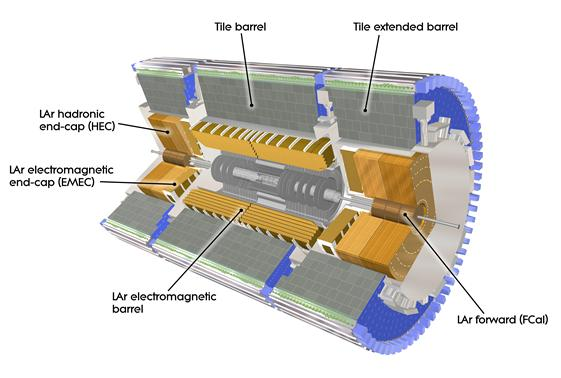
\includegraphics[scale=0.4]{Figures/dataset/cern_calorimeter.jpg}
    \caption{Représentation du calorimètre de l'expérience \acrshort{atlas} \cite{noauthor_computer_nodate}.}
    \label{fig:cern_calorimeter}
\end{figure}

Le détecteur est composé de plusieurs couches, comme visible sur la figure \ref{fig:calorimeter_structure}, qui possèdent chacune sa propre résolution. Les données issues de ces capteurs sont par la suite déroulées afin d'être représentées sur un plan à deux dimensions. C'est pourquoi nous retrouvons sur l'axe $\phi$ les valeurs allant de $-3.14$ à $3.14$ correspondant à $2\pi$ soit la circonférence du cylindre. Cela implique que les cellules aux coordonnées $\phi$ $-3.14$ et $3.14$ sont censées être plus proches entre elles que de la coordonnée $0$, de par le fait qu'elles sont issues d'un cylindre. Dans notre utilisation des données, afin de ne pas complexifier l'apprentissage de nos modèles pour la détection, nous ne prendrons pas en compte les jets présents dans ces extrémités.

\begin{figure}[hbt!]
    \centering
    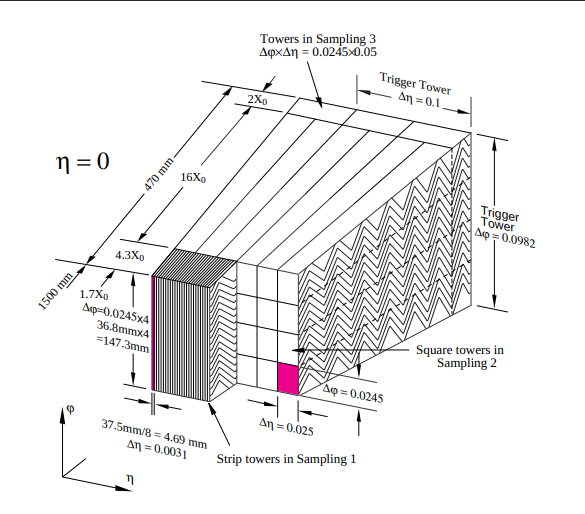
\includegraphics[scale=0.4]{Figures/dataset/structure_of_the_calorimeter.png}
    \caption{Structure du calorimètre de l'expérience \acrshort{atlas} \cite{noauthor_atlas_1996} (Figure 1-2).}
    \label{fig:calorimeter_structure}
\end{figure}

\break

En plus des données captées par des expériences réelles, le \acrshort{cern} possède un outil leur permettant de générer des simulations et d'indiquer les paramètres de leur choix. Ainsi, les données utilisées dans notre travail sont issues de ces simulations et nous ont été fournies directement par Claire Antel, post-doctorante à l'Université de Genève travaillant également sur le projet \acrshort{atlas} au \acrshort{cern}. Parmi celles-ci, le rayon des jets nous a été communiqué comme ayant été défini à $0.4$, et deux jeux de données nous ont été mis à disposition. Le premier contient un phénomène nommé "PileUp", tandis que le deuxième en est dépourvu.

Le "PileUp" apparaît lorsque plusieurs collisions de particules se produisent en même temps ou presque au sein du détecteur aux côtés de l'interaction d'intérêt. Les données obtenues lors d'une interaction d'intérêt peuvent alors être superposées aux valeurs liées à d'autres collisions. Les données "PileUp" sont plus proches de ce qu'une expérience réelle pourrait produire, mais ajoutent la complexité liée à la gestion du "PileUp".

Afin d'évaluer les performances pures des modèles utilisés face à la détection de jets, nous avons décidé d'utiliser les données ne contenant pas de "PileUp" dans notre travail.\\

Le jeu de données retenu est donc composé de vingt fichiers .h5. Ceux-ci sont divisés en deux catégories :

Dix d'entre eux contiennent les informations liées aux détections du calorimètre pour chaque expérience, comme ; les coordonnées $\eta \times \phi$, l'énergie, ou encore l'impulsion transverse des cellules.

Les dix autres sont liés aux fichiers précédents, et contiennent les informations relatives aux jets détectés dans chaque expérience, comme les coordonnées $\eta \times \phi$ de l'emplacement du jet.

Le premier ensemble nous permet de générer les images que nous passons à nos modèles, tandis que le deuxième nous sert à générer les labels à l'aide des coordonnées $\eta \times \phi$ des jets présents dans chaque expérience.

\section{Structure des fichiers}
\label{sec:files_structure}

Comme expliqué dans la section précédente \ref{sec:dataset_origin}, les données sont décomposées dans deux fichiers .h5 et retracent un total de mille expériences. Le premier contient toutes les informations relatives à la détection effectuées par le calorimètre. Et le second comporte les données liées aux jets détectés.

Dans le fichier des données du calorimètre, celui-ci possède l'objet nommé "caloCells" dans lequel nous retrouvons deux autres objets "1d" et "2d". Le premier inclut les éléments relatifs aux événements, tandis que le deuxième contient les données. C'est ce dernier qui nous intéresse. Nous allons parcourir les mille événements contenus dans l'objet "2d", qui possèdent une multitude d'informations, cependant dans le cadre de notre travail nous utiliserons uniquement les tableaux : $cell\_E$, l'énergie; $cell\_Sigma$, le niveau de bruit; $cell\_eta$, la coordonnée eta; $cell\_phi$, la coordonnée phi; et $cell\_pt$, l'impulsion transverse, qui contiennent les valeurs de chaque cellules.

Le fichier des informations des jets, possède la même structure initiale, avec d'autres tableaux contenant les valeurs des différents jets. Ces tableaux doivent tous posséder la même taille, or comme le nombre de jets peut varier d'une expérience à une autre, les tableaux sont définis à une taille fixe de trente. Le nombre de jets au sein des fichiers n'est jamais équivalent ou même proche de ce nombre comme nous pouvons le voir sur la figure \ref{fig:jet_distribution} . Concernant les variables utilisées, nous avons besoin des tableaux : $AntiKt4EMTopoJets\_eta$, la coordonnée $\eta$; et $AntiKt4EMTopoJets\_phi$ la coordonnée $\phi$, qui contiennent soit les coordonnées des jets de l'expérience courante, soit la valeur $nan$ pour compléter le tableau.

\begin{figure}[hbt!]
    \centering
    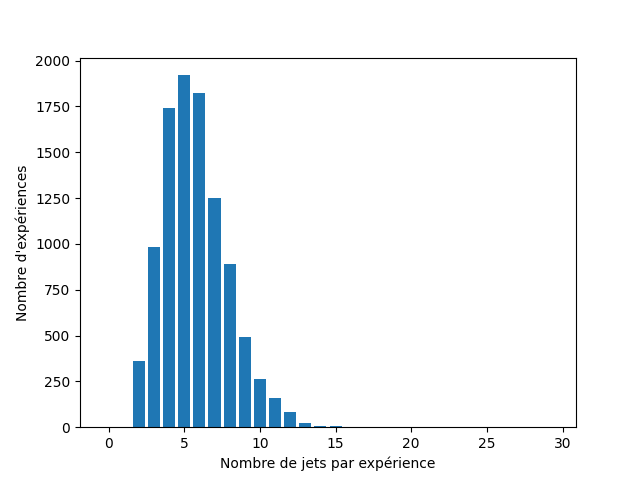
\includegraphics[scale=0.7]{Figures/dataset/file_jet_distribution.png}
    \caption{Distribution du nombre de jets par expérience à partir des fichiers de données utilisés}
    \label{fig:jet_distribution}
\end{figure}

Il reste évidemment beaucoup d'informations à disposition dans ces fichiers, néanmoins, dans notre cadre, nous nous contentons d'utiliser celles que nous avons indiquées.

\section{Prise en main des données issues du calorimètre}

Avant de pouvoir générer des images et des labels pour nos modèles, il nous a d'abord fallu prendre en main les données, les comprendre, les nettoyer, et les manipuler afin d'en extraire l'essence.

Pour cela, nous avons tout d'abord débuté en affichant sur un plan à deux dimensions les emplacements des capteurs comme visible sur la figure \ref{fig:calocells_location}. Nous voyons que l'emplacement des capteurs n'est pas régulier sur l'ensemble du calorimètre, et qu'il pourrait être par conséquent plus complexe de réaliser des détections de jets dans les zones moins fournies en capteurs. En revanche, nous constatons que la région dans l'intervalle $\eta \in \mathbb{R} : \eta \in [-2.4;2.4]$ et $\phi \in \mathbb{R} : \phi \in [-3.14;3.14]$ possède des capteurs disposés plus régulièrement.

\begin{figure}[hbt!]
    \centering
    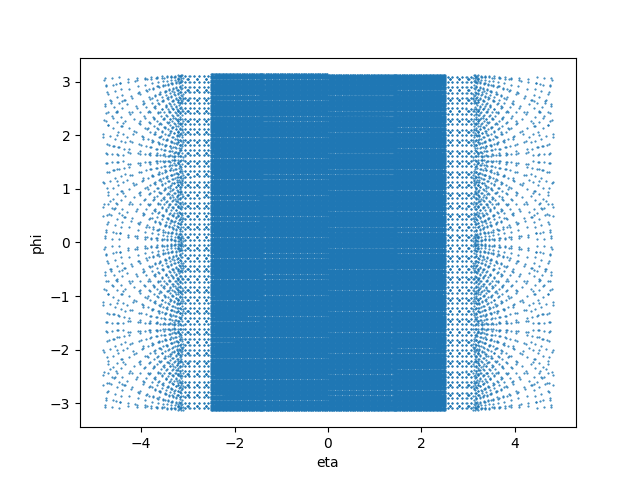
\includegraphics[scale=0.7]{Figures/dataset/calorimeter_cells.png}
    \caption{Emplacement des cellules du calorimètre}
    \label{fig:calocells_location}
\end{figure}

En nous concentrant sur l'intervalle défini, nous pouvons voir sur la figure \ref{fig:calocells_location_eta_reduced} que deux zones verticales symétriques moins denses en capteurs apparaissent vers $\eta$ $-1.45$ et $1.45$. Cela n'est pas critique, mais il est bon de noter que plus tard, lors de la création d'une matrice à partir des données du calorimètre, des artéfacts peuvent en résulter. Ces derniers sont des anomalies non souhaitées et qui ne sont pas représentatives de ce que nous souhaitons étudier. Dans notre cas, ils peuvent apparaître de par la disposition des capteurs, et venir complexifier voire fausser les résultats de nos modèles en leur faisant apprendre des caractéristiques non pertinentes.

\begin{figure}[hbt!]
    \centering
    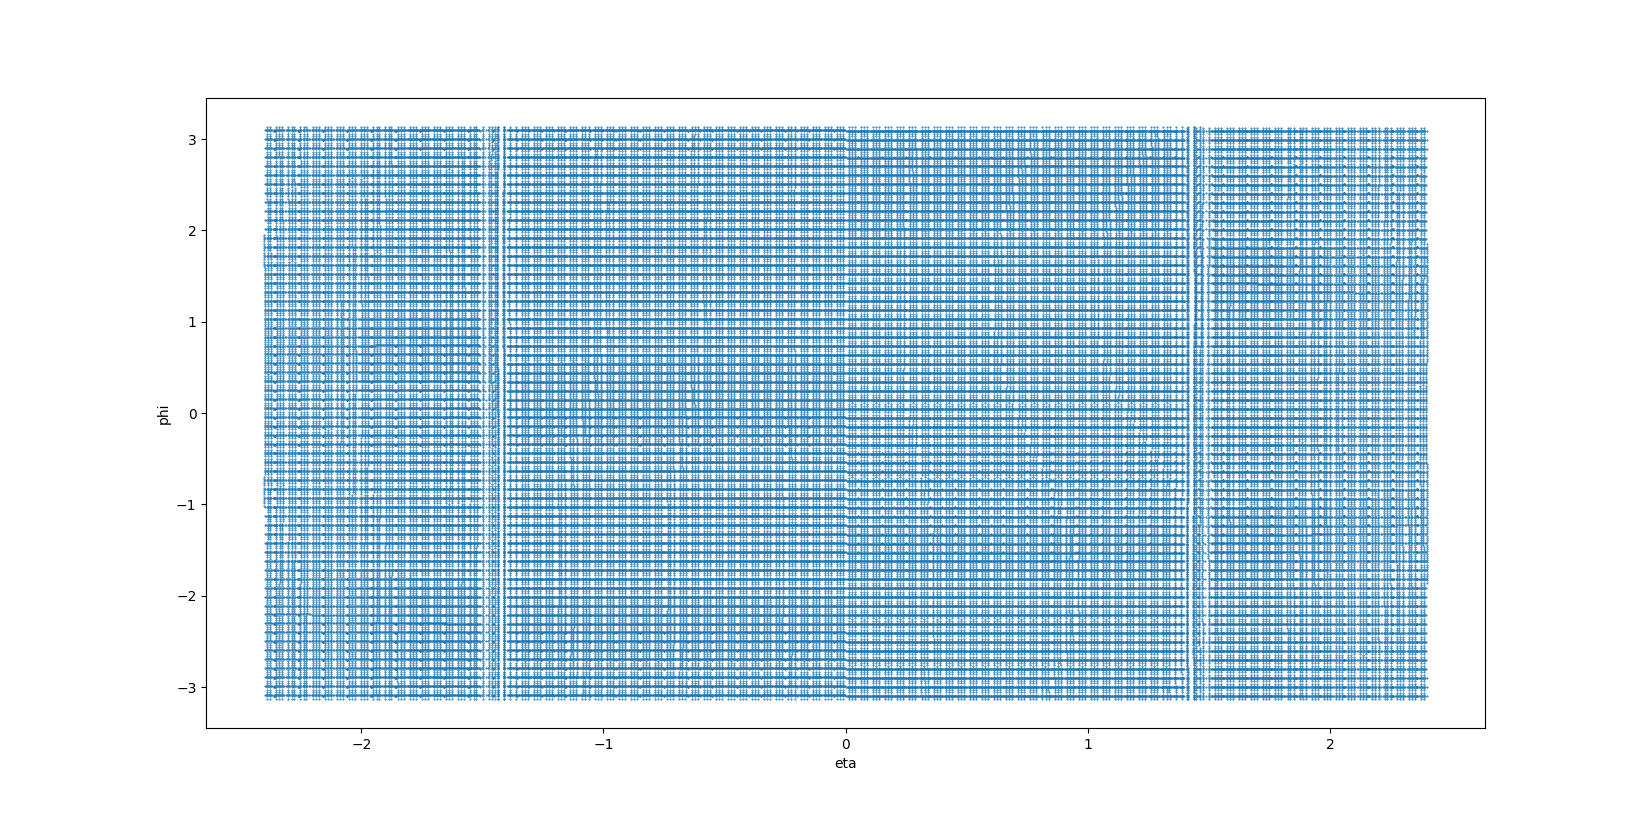
\includegraphics[scale=0.3]{Figures/dataset/calorimeter_cells_eta_reduced.png}
    \caption{Emplacement des cellules du calorimètre dans l'intervalle $\eta \in \mathbb{R} : \eta \in [-2.4;2.4]$ et $\phi \in \mathbb{R} : \phi \in [-3.14;3.14]$}
    \label{fig:calocells_location_eta_reduced}
\end{figure}

\break

En agrandissant la région dense en capteurs autour de $0$, nous voyons comment ceux-ci sont répartis grâce à la figure \ref{fig:calocells_location_eta_reduced_zoomed_in}. Nous constatons qu'ils ne sont pas tous disposés à distance égale les un des autres, étant donné qu'ils correspondent aux différentes couches de capteurs possédant une granularité différente. Il est important de prendre en compte cette répartition, car cela peut être une source d'artéfacts sur l'image générée à partir des données.

\begin{figure}[hbt!]
    \centering
    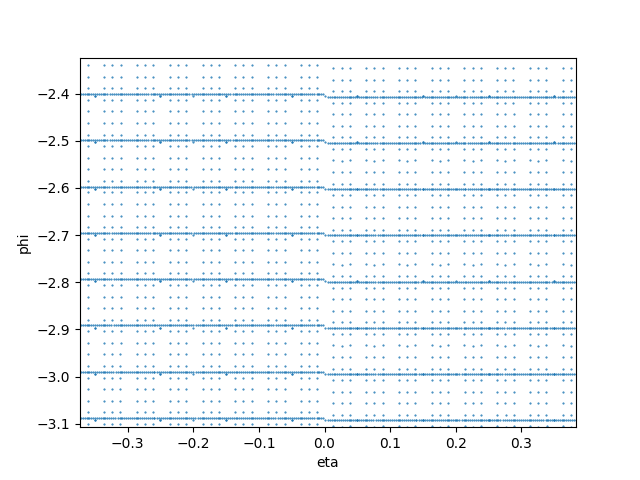
\includegraphics[scale=0.7]{Figures/dataset/calo_cells_zoomed_in.png}
    \caption{Emplacement des cellules du calorimètre zoomé}
    \label{fig:calocells_location_eta_reduced_zoomed_in}
\end{figure}

\break

\section{Manipulation et préparation des données issues du calorimètre}

\subsection{Création d'une matrice}

L'étape suivant la visualisation de l'emplacement des capteurs du calorimètre consiste à réaliser une matrice pour représenter celle-ci. Pour ce faire, nous avons besoin de connaître la distance entre deux capteurs. Après une discussion avec la professeure Anna Sfyrla de l'Université de Genève travaillant également au \acrshort{cern} sur le projet \acrshort{atlas}, il en est ressorti d'utiliser une distance de $0.025$ pour $\eta$ et $\phi$ correspondant au "Sampling 2" du calorimètre \cite{noauthor_atlas_1996}.

À partir de cette information nous pouvons donc construire une matrice utilisant un pas de $0.025$ sur l'intervalle $\eta \in \mathbb{R} : \eta \in [-2.4;2.4]$ et $\phi \in \mathbb{R} : \phi \in [-3.14;3.14]$. La taille de celle-ci est de $\eta \times \phi = 193 \times 253$. Afin de pouvoir y insérer des valeurs, nous commençons par arrondir les coordonnées $\eta \times \phi$ à 0.025, puis à l'aide des transformations suivantes :

\label{formula:compute_indices}

\[Indice \: \eta \: Cell_{i} = (Cell_{i_{\eta}} + 2.4) / (2.4*2) \cdot (W-1)\]
\[Indice \: \phi \: Cell_{i} = (Cell_{i_{\phi}} + 3.15) / (3.15*2) \cdot (H-1)\]

où $W$ et $H$ correspondent respectivement à la taille de la matrice pour $\eta$ et $\phi$. Nous calculons les indices $\eta \times \phi$ pour notre matrice de la cellule $i$ à partir des coordonnées arrondies. Notons que nous utilisons pour $\phi$ la valeur de $3.15$ que nous avons obtenu en arrondissant $\pi$ vers le haut.

Nous pouvons à présent ajouter à chaque indice de notre matrice l'énergie de chaque cellule. Étant donné que nous avons réalisé un arrondi sur les coordonnées, nous allons additionner les valeurs dans un même indice afin de ne pas perdre d'énergie lors de la transformation.\\

\subsection{Normalisation de l'énergie avec le niveau de bruit et filtrage des données}

L'énergie en provenance du calorimètre contient également le bruit de la cellule en question. Afin de normaliser les valeurs de celles-ci, nous divisons l'énergie par le niveau de bruit pour en faire ressortir le signal. Cette méthode nous permet d'obtenir un ratio utile pour comparer les cellules, mais surtout de distinguer les signaux pertinents du bruit de fond.

Si nous observons à quoi ressemble une de nos matrices actuellement, nous obtenons un résultat similaire à celui de la figure \ref{fig:matrix_post_energy_over_noise_no_filter}. Nous y voyons quelques pixels ressortir, ainsi qu'une échelle d'énergie sur bruit très élevée. Bien que cela soit un début, nous faisons face à deux problèmes; les cellules contenant peu d'énergie sur bruit ne sont pas visibles, et entre deux expériences cette valeur peut énormément varier.

\begin{figure}[hbt!]
    \centering
    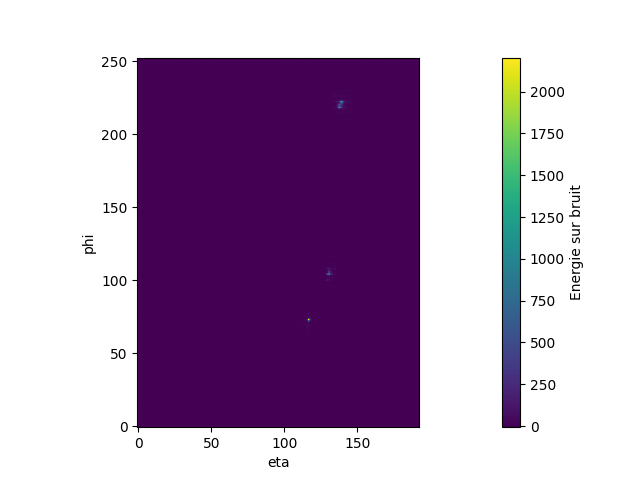
\includegraphics[scale=0.7]{Figures/dataset/matrix_post_energy_over_noise_no_filter.png}
    \caption{Matrice générée à partir de l'énergie sur bruit des cellules du calorimètre pour l'expérience 0 du fichier : \url{user.cantel.33075755.\_000001.calocellD3PD\_mc16\_JZW4.r14423}.}
    \label{fig:matrix_post_energy_over_noise_no_filter}
\end{figure}

\break

La distribution de l'énergie sur bruit supérieure à $0$ de chaque cellule de toutes les expériences du fichier $user.cantel.33075755.\_000001.calocellD3PD\_mc16\_JZW4.r14423$ visible sur la figure \ref{fig:hist_energy_over_sigma}, nous montre que la majorité d'entre elles possèdent une énergie sur bruit relativement faible. Ainsi, même si les cellules avec une valeur très élevée sont intéressantes, il ne faut pas pour autant négliger celles dont l'énergie sur bruit est plus modeste.

\begin{figure}[hbt!]
    \centering
    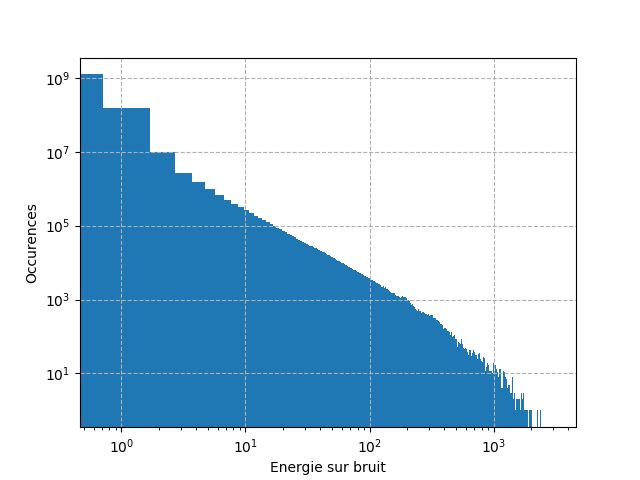
\includegraphics[scale=0.7]{Figures/dataset/hist_energy_over_sigma.png}
    \caption{Histogramme de l'énergie sur bruit supérieure à 0 de toutes les cellules parmis toutes les expériences du fichier : \url{user.cantel.33075755.\_000001.calocellD3PD\_mc16\_JZW4.r14423}.}
    \label{fig:hist_energy_over_sigma}
\end{figure}

\break

Pour limiter la quantité d'énergie sur bruit maximum qu'une cellule peut atteindre dans le but de rendre les autres valeurs plus visibles, mais également afin d'éliminer les faibles valeurs pouvant être confondues avec du bruit, nous définissons deux seuils.

Le premier va retirer les cellules dont l'énergie sur bruit est inférieure à une valeur donnée. Tandis que le second fixe une valeur maximum qui est attribuée à toutes celles la dépassant. Cela a pour but d'éviter que des cellules très énergétiques en "cachent" d'autres sur notre matrice.

Les valeurs définies pour les seuils nous ont été indiquées par la Professeure Anna Sfyrla. Nous utilisons exclusivement les valeurs pour lesquelles l'énergie sur bruit est supérieure à $2$ (qui est également celle recommandée par le CERN \cite{gross_frequentist_2011}). Quant à la valeur maximum qui peut être attribuée à une cellule, celle-ci est définie à $6$, légèrement au-dessus du traditionnel seuil de $5$ \cite{lyons_discovering_2013}.\\

Visualisons à présent notre matrice représentée à la figure \ref{fig:matrix_post_energy_over_noise} construite en utilisant nos seuils, et sur laquelle des cercles rouges correspondent à l'emplacement des jets. Même si cela n'est pas très visible, nous voyons quelques cellules en plus, et surtout une échelle d'énergie sur bruit bien plus petite que sur la figure \ref{fig:matrix_post_energy_over_noise_no_filter}. Cependant, nous n'avons toujours pas résolu nos deux problèmes précédents. En effet, même si la valeur maximum d'une cellule est fixée à $6$, sur notre matrice nous additionnons les valeurs des cellules correspondant aux mêmes indices. Cette façon de faire implique que certains indices peuvent posséder des valeurs encore trop élevées cachant ainsi ceux à l'énergie sur bruit plus faible.

\begin{figure}[hbt!]
    \centering
    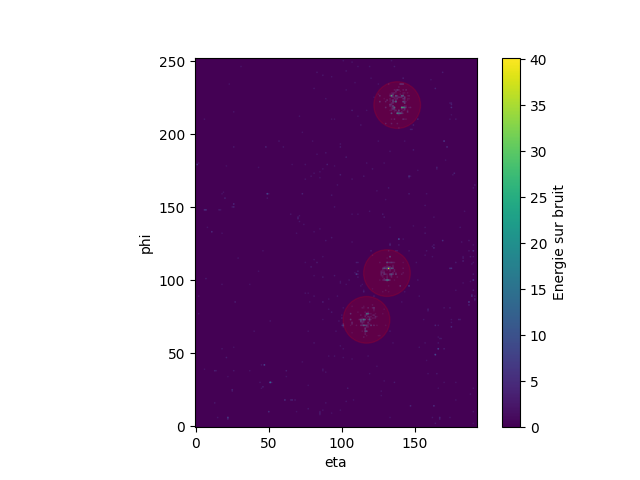
\includegraphics[scale=0.7]{Figures/dataset/matrix_post_energy_over_noise.png}
    \caption{Matrice générée à partir de l'énergie sur bruit filtrée des cellules du calorimètre supérieure à 2 pour l'expérience 0 du fichier : \url{user.cantel.33075755.\_000001.calocellD3PD\_mc16\_JZW4.r14423}.}
    \label{fig:matrix_post_energy_over_noise}
\end{figure}

\break

\subsection{Normalisation des matrices entre 0 et 1}

Afin de remédier à ces problèmes, nous normalisons nos valeurs pour qu'elles soient contenues entre $0$ et $1$. Pour cela, nous souhaitons utiliser une fonction non linéaire qui va accentuer le rôle des cellules avec des valeurs plus faibles, tout en réduisant l'impact des valeurs très élevées. Étant donné que grâce à nos seuils nos valeurs sont toujours positives, une fonction parfaite pour ce rôle serait le logarithme. Néanmoins, en gardant en tête que nous souhaitons implémenter tout cela sur \acrshort{fpga}, la fonction logarithmique étant très coûteuse, nous allons utiliser une alternative. La fonction retenue est :

\[f(x) = 1-\frac{(\mu+\sigma)}{((\mu+\sigma)+x)}\]

où $\mu$ et $\sigma$ correspondent respectivement à la moyenne et à l'écart-type des énergies sur bruit de toutes les cellules. Comme nous pouvons le voir sur la figure \ref{fig:personalized_function}, celle-ci nous assure que nos valeurs positives le restent, tout en donnant de l'importance aux faibles valeurs, et en diminuant l'impact des grandes. Par ailleurs, en utilisant la moyenne et l'écart-type de l'expérience en cours, cela nous permet d'adapter notre fonction pour que son comportement s'adapte aux valeurs rencontrées.

\begin{figure}[hbt!]
    \centering
    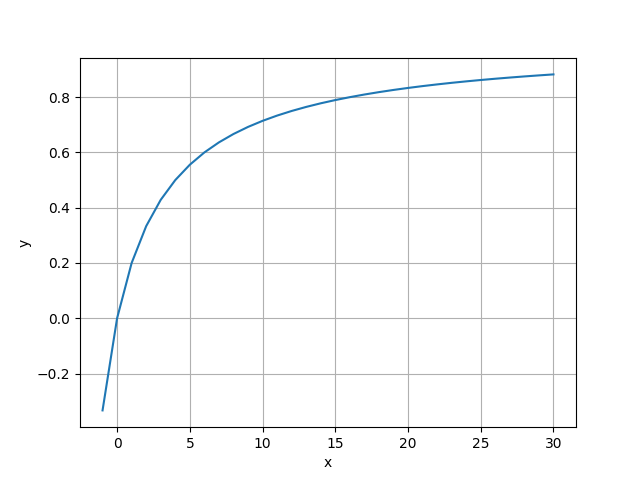
\includegraphics[scale=0.7]{Figures/dataset/personalized_function.png}
    \caption{Visualisation de la fonction utilisée pour normaliser les valeurs d'énergie sur bruit : $f(x) = 1-(\mu+\sigma)/((\mu+\sigma)+x)$ où $\mu$ est défini à $5$ et $\sigma$ à 1.}
    \label{fig:personalized_function}
\end{figure}

L'application de notre fonction sur notre matrice de la figure \ref{fig:matrix_post_energy_over_noise} nous donne le résultat affiché sur la figure \ref{fig:matrix_post_energy_over_noise_normalized}. Nous voyons à présent sur celle-ci que les zones contenant des jets ressortent beaucoup mieux et sont plus facilement identifiables. Par ailleurs, nous constatons aussi que d'autres cellules contenant de l'énergie sur bruit de façon beaucoup moins intense deviennent visibles.

L'utilisation de notre fonction nous démontre ses biens faits, et la place importante qu'elle occupe dans la préparation des données.

\begin{figure}[hbt!]
    \centering
    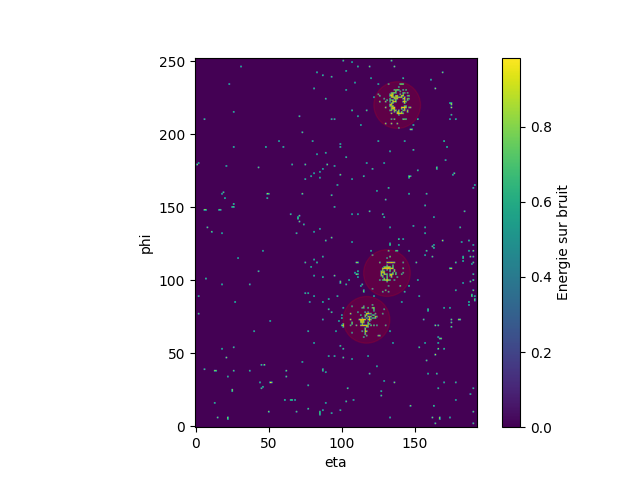
\includegraphics[scale=0.7]{Figures/dataset/matrix_post_energy_over_noise_normalized.png}
    \caption{Matrice générée à partir de l'énergie sur bruit des cellules du calorimètre supérieure à 2 puis normalisée pour l'expérience 0 du fichier : \url{user.cantel.33075755.\_000001.calocellD3PD\_mc16\_JZW4.r14423}.}
    \label{fig:matrix_post_energy_over_noise_normalized}
\end{figure}

\break

\subsection{Utilisation de canaux}

Bien que notre préparation des données semble faire correspondre les jets aux zones où des groupes de cellules possèdent une énergie sur bruit plus élevé, nous remarquons sur la figure \ref{fig:matrix_post_energy_over_noise_normalized_not_all_jets_visible} que certains d'entre eux, bien qu'indiqués présents, ne semblent pas ressortir. C'est le cas notamment pour le jet défini environ aux coordonnées $\eta \times \phi = 139 \times 220$. Celui-ci possède quelques cellules avec des valeurs autour de $0.8$ mais cela n'est pas fondamentalement différent d'autres zones de notre matrice qui ne contiennent pas de jets.

Ainsi, l'énergie sur bruit ne semble pas suffisante à elle seule afin de réaliser la détection de jets. Dans l'article traitant de l'algorithme $anti-k_t$ \cite{cacciari_anti-k_t_2008} réalisant des regroupements de ces derniers, l'impulsion transverse que nous possédons dans notre jeu de données est utilisée.

Sur la figure \ref{fig:matrix_post_energy_over_noise_normalized_not_all_jets_visible_e_o_n_and_pt}, nous pouvons observer la zone du jet vue par les deux matrices issues de l'énergie sur bruit à gauche, et de l'impulsion transverse à droite. Bien qu'il s'agisse des mêmes cellules concernées, nous pouvons voir que les valeurs de celles-ci sont différentes.

Utiliser les deux matrices ainsi générées pourrait être bénéfique pour l'apprentissage et la détection de jets par nos modèles.

Nous créons donc une matrice contenant trois canaux afin de pouvoir l'utiliser comme une image. Le premier canal contient les valeurs de l'énergie sur bruit normalisées. Le deuxième est constitué de l'impulsion transverse normalisée. Et finalement, le troisième est un canal vide rempli par des zéros. Cette dernière pourrait potentiellement accueillir d'autres valeurs pertinentes pour la détection de jets. 

\begin{figure}[hbt!]
    \centering
    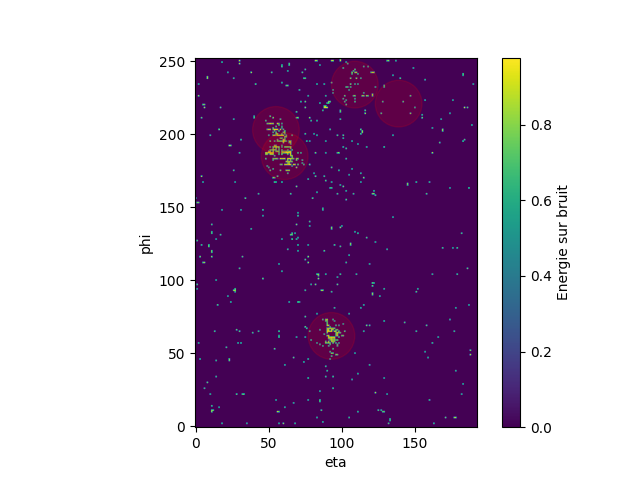
\includegraphics[scale=0.7]{Figures/dataset/matrix_post_energy_over_noise_normalized_not_all_jets_visible.png}
    \caption{Matrice générée à partir de l'énergie sur bruit des cellules du calorimètre supérieure à 2 puis normalisée pour l'expérience 9 du fichier : \url{user.cantel.33075755.\_000001.calocellD3PD\_mc16\_JZW4.r14423}.}
    \label{fig:matrix_post_energy_over_noise_normalized_not_all_jets_visible}
\end{figure}

\begin{figure}[hbt!]
    \centering
    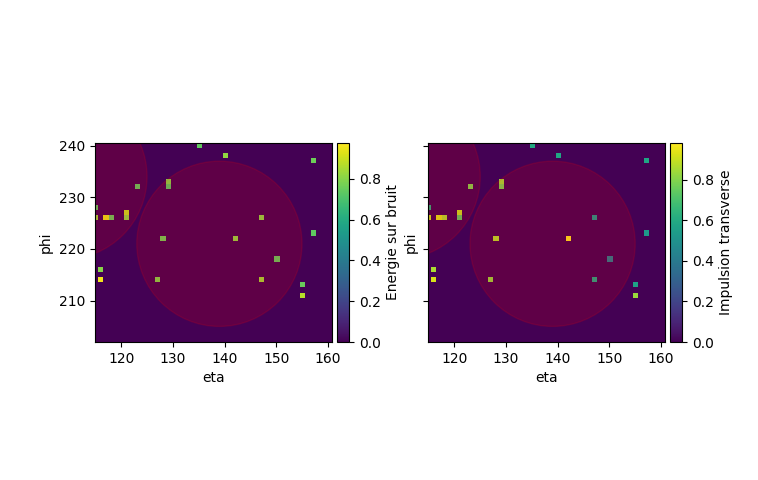
\includegraphics[scale=0.7]{Figures/dataset/matrix_post_energy_over_noise_normalized_not_all_jets_visible_e_o_n_and_pt.png}
    \caption{Matrices générées à partir de l'énergie sur bruit (à gauche) et de l'impulsion transverse (à droite) des cellules du calorimètre supérieure à $2$ puis normalisées pour l'expérience 9 du fichier : \url{user.cantel.33075755.\_000001.calocellD3PD\_mc16\_JZW4.r14423}.}
    \label{fig:matrix_post_energy_over_noise_normalized_not_all_jets_visible_e_o_n_and_pt}
\end{figure}

\break

\subsection{Gestion des artéfacts}

Même s'ils ne sont pas clairement visibles, les images générées jusqu'à présent contiennent des artéfacts. Ceux-ci deviennent visibles lorsque nous diminuons le seuil des valeurs acceptées dans notre matrice. En le passant de $2$ à $0$, nous obtenons le résultat de la figure \ref{fig:matrix_post_traitement_artefacts}. Grâce à la normalisation, précédemment appliquée, nous pouvons y voir apparaître des lignes verticales symétriques, ainsi que des lignes horizontales régulières qui ne sont pas sans nous rappeler la disposition des capteurs du calorimètre.

\begin{figure}[hbt!]
    \centering
    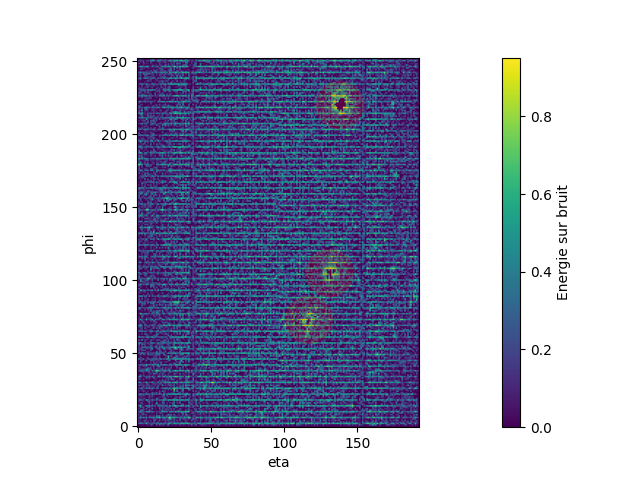
\includegraphics[scale=0.7]{Figures/dataset/matrix_post_traitement_artefacts.png}
    \caption{Matrice générée à partir de l'énergie sur bruit des cellules du calorimètre supérieure à 0 puis normalisée pour l'expérience 0 du fichier : \url{user.cantel.33075755.\_000001.calocellD3PD\_mc16\_JZW4.r14423}.}
    \label{fig:matrix_post_traitement_artefacts}
\end{figure}

\break

Une approche qui nous a été conseillée par Leon Bozianu, doctorant à l'Université de Genève dans l'équipe de la professeure Anna Sfyrla, était d'utiliser une distance entre les capteurs égale à $\delta \eta \times \delta \phi = 0.1 \times 0.1$ correspondant à la plus grande granularité des capteurs.

En diminuant la granularité de notre matrice, mais en conservant l'énergie sur bruit des cellules supérieures à $0$, nous obtenons des matrices comme celle de la figure \ref{fig:matrix_post_traitement_reduced_0} d'une taille de $\eta \times \phi = 49 \times 64$. Certains artéfacts sont toujours présents, mais de façon plus nuancée.

\begin{figure}[hbt!]
    \centering
    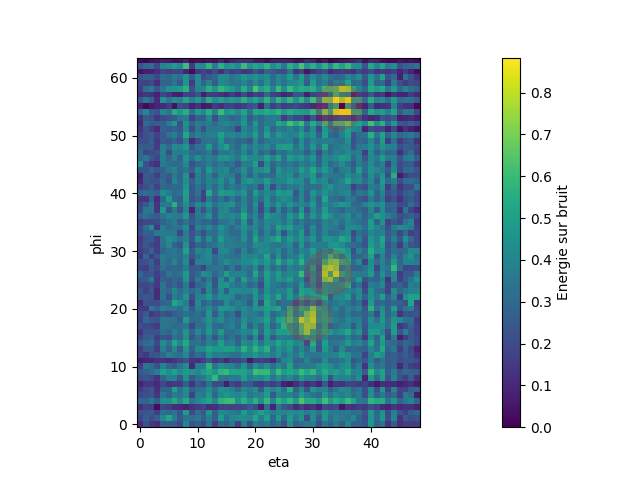
\includegraphics[scale=0.7]{Figures/dataset/matrix_post_traitement_reduced_0.png}
    \caption{Matrice d'un pas de $0.1 \times 0.1$ générée à partir de l'énergie sur bruit des cellules du calorimètre supérieure à 0 puis normalisée pour l'expérience 0 du fichier : \url{user.cantel.33075755.\_000001.calocellD3PD\_mc16\_JZW4.r14423}.}
    \label{fig:matrix_post_traitement_reduced_0}
\end{figure}

\break

En conservant exclusivement les cellules dont l'énergie sur bruit est supérieure ou égale à $2$, nous voyons, comme sur la figure \ref{fig:matrix_post_traitement_reduced_2}, que les zones contenant des jets ressortent bien et qu'elles sont moins sujettes à l'impact des artéfacts.

\begin{figure}[hbt!]
    \centering
    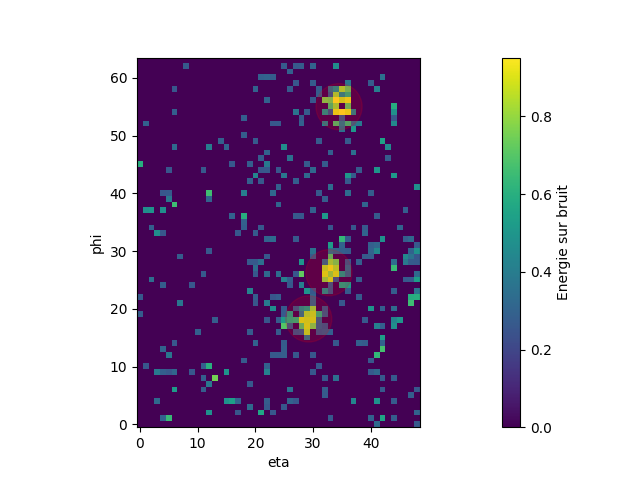
\includegraphics[scale=0.7]{Figures/dataset/matrix_post_traitement_reduced_2.png}
    \caption{Matrice d'un pas de $0.1 \times 0.1$ générée à partir de l'énergie sur bruit des cellules du calorimètre supérieure à 2 puis normalisée pour l'expérience 0 du fichier : \url{user.cantel.33075755.\_000001.calocellD3PD\_mc16\_JZW4.r14423}.}
    \label{fig:matrix_post_traitement_reduced_2}
\end{figure}

\break

\subsection{Sauvegarde des matrices}

Après toutes les étapes précédentes, nous souhaitons conserver nos matrices pour pouvoir les utiliser par la suite pour l'entraînement et l'évaluation de nos modèles.

Afin de les sauvegarder dans un format facilement utilisable et commun à de nombreux réseaux neuronaux convolutifs, nous avons décidé de multiplier toutes les valeurs de nos matrices par $255$ afin de les contenir sur $8$ bits. Grâce aux trois canaux de celles-ci, nous pouvons les représenter sous forme d'images.

Par ailleurs, il est important de n'appliquer aucune compression sur les images pour éviter de les détériorer ou d'introduire des artéfacts. Le résultat de toutes les manipulations et préparations de nos données nous donne des images semblables à la figure \ref{fig:image_type_from_dataset_49x64}.

\begin{figure}[hbt!]
    \centering
    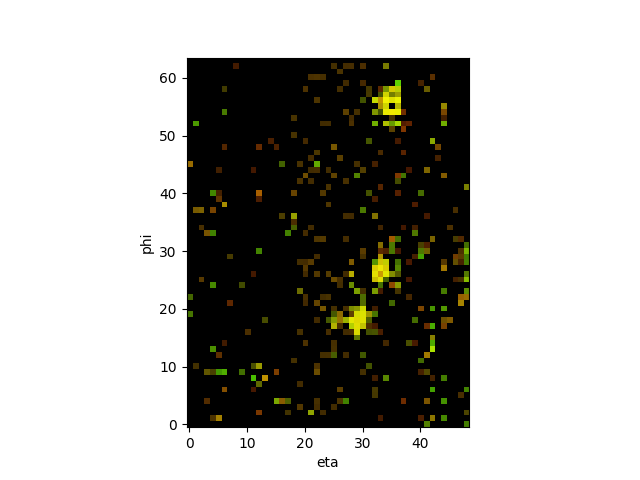
\includegraphics[scale=0.7]{Figures/dataset/image_type_from_dataset_49x64.png}
    \caption{Image construite à partir du jeu de donnée pour l'expérience 0 du fichier : \url{user.cantel.33075755.\_000001.calocellD3PD\_mc16\_JZW4.r14423}.}
    \label{fig:image_type_from_dataset_49x64}
\end{figure}

\break

Lors de ce travail, plutôt que de travailler avec des dossiers d'images, nous avons enregistré nos matrices dans des fichiers binaires .npy. Ce dernier est un format proposé par la librairie NumPy permettant d'enregistrer des tableaux facilement, et d'utiliser peu de mémoire.


\section{Manipulation et préparation des données issues des jets}

En ce qui concerne les données des jets, comme décrit dans la section \ref{sec:files_structure} nous allons utiliser les coordonnées $\eta \times \phi$ afin de calculer les indices correspondant sur nos matrices à l'aide de la même formule décrite dans la sous-section \ref{formula:compute_indices}.

Tout comme pour les données du calorimètre, nous n'utilisons que celles comprises dans l'intervalle $\eta \in \mathbb{R} : \eta \in [-2.4;2.4]$ et $\phi \in \mathbb{R} : \phi \in [-3.14;3.14]$.\\

Les données des jets sont utilisées pour générer des labels. Puisque la génération de ces derniers est différente en fonction du modèle, les explications à leur sujet sont comprises dans le chapitre traitant des modèles utilisés \ref{UsedModels}, aux sous-chapitres : \ref{subsec:yolov8_labels_generation} et \ref{subsec:resnet18+head_label_generation}.

\section{Répartition des données utilisées}

Comme indiqué initialement dans la section sur la provenance des données \ref{sec:dataset_origin}, nous possédons dix fichiers de données du calorimètre, et dix autres contenant les jets associés.

Chaque fichier contient $1000$ expériences. Ainsi, nous travaillons avec un total de $10'000$ événements. Nous avons décidé d'en sélectionner $8'000$ pour l'entraînement de nos modèles, $1'000$ sont dédiés pour la validation, et finalement les $1'000$ derniers sont utilisés comme ensemble de test. 

La sélection de ces derniers a été réalisée simplement à l'aide d'un modulo. Toutes les cinq expériences, un événement est ajouté alternativement à l'ensemble de validation ou de test.

\section{Choix des modèles de machine learning}

Initialement, notre projet devait utiliser le modèle de segmentation sémantique U-Net. En imaginant le bon fonctionnement du modèle sur les entrées, nous aurions en sortie un masque contenant les pixels appartenant aux jets, ceux correspondant aux bords des jets, ainsi que le fond.

Bien que cela soit une approche viable, en discutant plus en détail avec la professeure Anna Sfyrla de l'utilisation de la sortie du modèle, nous avons découvert les points suivants.

Outre la contrainte de vitesse, une expérience est considérée comme intéressante ou non en fonction du nombre de jets qu'elle contient et de l'énergie de ceux-ci. Il est donc pertinent d'anticiper comment la sortie va être traitée afin d'obtenir le nombre de jets et leur énergie respective. Même s'il est possible de calculer ces valeurs à partir d'un masque, il demeure plus simple et plus rapide de le faire à partir des coordonnées du centre d'un jet. Cela évite de lire chaque pixel issu du masque pour savoir s'il doit être pris en compte ou non. De plus, comme il s'agit de segmentation sémantique, nous savons uniquement si le pixel en question appartient ou non à la classe jet mais pas à quel jet, il faut donc en plus gérer cela.

C'est pour les raisons précédentes que nous utilisons des modèles de détection nous retournant le centre des jets détectés. Leur choix sera détaillé dans le chapitre qui leur est dédié (\ref{UsedModels}).

%----------------------------------------------------------------------------------------

% HLS4ML

\chapter{HLS4ML} % Main chapter title

\label{HLS4ML} % For referencing the chapter elsewhere, use \ref{HLS4ML} 

%----------------------------------------------------------------------------------------

\section{Description de HLS4ML}

Le paquet \acrshort{hls4ml} est un outil publié en juin 2018 par Javier Duartea et al., ayant pour but de traduire des modèles de machine learning développés en Python à l'aide de bibliothèques comme Keras ou Pytorch, en code VHDL ou Verilog pour \acrshort{fpga} \cite{duarte_fast_2018}.

Au fil du temps, ce dernier a été étendu et amélioré notamment pour son utilisation avec des réseaux neuronaux convolutifs \cite{aarrestad_fast_2021} et \cite{ghielmetti_real-time_2022}.

En plus de proposer des implémentations de faible latence, \acrshort{hls4ml} permet de développer rapidement des prototypes de modèles de machine learning sans de grandes connaissances des langages VHDL ou Verilog, tout en préservant les ressources matérielles disponibles.

\section{HLS4ML et Vitis HLS}

Comme son nom l'indique, l'outil \acrfull{hls4ml} fonctionne conjointement avec Vitis \acrfull{hls}. En effet, lors du flux de travail que nous verrons plus en détail à la section suivante (\ref{hls4ml_workflow}), le code Python est transformé en code C++ qui est converti en un projet \acrshort{hls} puis synthétisé en code VHDL ou Verilog. Bien qu'il existe différents outils pour gérer des projets \acrshort{hls}, nous nous concentrerons sur Vitis \acrshort{hls} qui est officiellement supporté par \acrshort{hls4ml} bien qu'encore au stade expérimental.

\acrfull{hls} est un processus de conception qui à partir d'un code écrit en ANSI C, ou C++ est capable de transformer celui-ci en \acrfull{rtl} (une méthode de conception de circuits logique) à l'aide d'un langage de description matérielle tel que VHDL ou Verilog. Ce dernier peut être alors synthétisé et implémenté sur \acrshort{fpga}.\\

Vitis \acrshort{hls} permet de développer des algorithmes sans avoir besoin d'écrire de code dans un langage de description matérielle, et ainsi d'accélérer la phase de conception. Par ailleurs, il fournit également des directives spéciales nommées pragmas permettant de contrôler et d'optimiser la synthèse du code. Un exemple de ces derniers pourrait être le pragma \textbf{HLS pipeline} qui va réduire la latence en parallélisant les commandes de la chaîne de traitement. Ainsi, comme illustré sur la figure \ref{fig:pipeline_pragma} dans le cas (B), les instructions sont organisées de manière à ce que différentes opérations soient réalisées en parallèle, plutôt que séquentiellement.

\begin{figure}[hbt!]
    \centering
    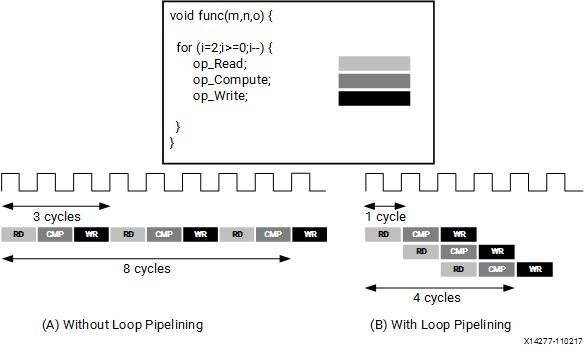
\includegraphics[scale=0.9]{Figures/hls4ml/pipeline_pragma.png}
    \caption{Exemple d'une pipeline de boucle \cite{noauthor_tme1532103642766image_nodate}.}
    \label{fig:pipeline_pragma}
\end{figure}

\break

\section{Flux de travail}
\label{hls4ml_workflow}

Le fonctionnement de \acrshort{hls4ml} peut être simplement décrit à l'aide du schéma suivant \ref{fig:hls4ml_workflow} :

\begin{figure}[hbt!]
    \centering
    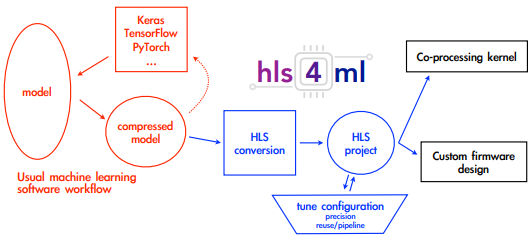
\includegraphics[scale=0.7]{Figures/hls4ml/hls4ml_workflow.png}
    \caption{Flux de travail typique lors de la conversion d'un modèle vers une implémentation \acrshort{fpga} avec \acrshort{hls4ml} \cite{duarte_fast_2018} (Figure 1)}
    \label{fig:hls4ml_workflow}
\end{figure}

Celui-ci débute par la partie illustrée en rouge, et représente les étapes habituelles de conception d'un réseau de neurones pour une tâche spécifique. Celles-ci sont réalisées avec des outils comme (Q)Keras, Tensorflow, ou Pytorch et impliquent des étapes d'entraînement, de quantification ou encore de compression avant d'obtenir le modèle final.

Le flux passe alors dans la section en bleu et converti le modèle de machine learning à l'aide de \acrshort{hls4ml} en un projet \acrshort{hls}. Celui-ci pourra être synthétisé et implémenté par la suite sur \acrshort{fpga} comme indiqué par la partie en noir.

\acrshort{hls4ml} possède un nombre de paramètres configurables afin de personnaliser au mieux la latence, l'intervalle d'initiation, ou encore les ressources utilisées par le résultat final.

\section{Fonctions (Q)Keras supportées}

Lors de la réalisation de notre travail, nous avons utilisé la version 0.7.1 de hls4ml. Bien que celle-ci propose le support de différentes bibliothèques, seule (Q)Keras est convenablement supportée, les autres étant limitées ou en cours de développement. Voici la liste des couches supportées avec la version utilisée extraite directement du code : \\

\begin{itemize}

\item\textbf{Entrée} : InputLayer.\\

\item\textbf{Convolution} : Conv1D, SeparableConv1D, Conv2D, SeparableConv2D, DepthwiseConv2D, QConv1D, QConv2D.\\

\item\textbf{Pooling} : MaxPooling1D, MaxPooling2D, AveragePooling1D, AveragePooling2D, GlobalMaxPooling1D, GlobalMaxPooling2D, GlobalAveragePooling1D, GlobalAveragePooling2D.\\

\item\textbf{Activation} : Activation, LeakyReLU, ThresholdedReLU, ELU, PReLU, Softmax, ReLU, QActivation.\\

\item\textbf{Normalisation} : BatchNormalization, QBatchNormalization.\\

\item\textbf{Dense} : Dense, QDense, BinaryDense, TernaryDense.\\

\item\textbf{Redimensionnement} : ZeroPadding1D, ZeroPadding2D, Flatten, Reshape, Permute.\\

\item\textbf{Autres} : QConv2DBatchnorm, UpSampling1D, UpSampling2D, Embedding, GarNet, GarNetStack, SimpleRNN, LSTM, GRU, Add, Subtract, Multiply, Average, Maximum, Minimum, Concatenate, Dot.\\

\end{itemize}

Dans notre cas, toutes les couches de notre modèle ResNet18+Tête sont supportées. Néanmoins, cela n'est pas le cas pour l'implémentation de YOLOv8 par KerasCV. Dans ce cas, il aurait été possible de les ajouter manuellement à l'aide de l'"extension API" \cite{noauthor_extension_nodate}. Cette dernière permet de définir la couche spécifique en la développant selon les critères de \acrshort{hls4ml} en Python et en C++.

\section{Limitations rencontrées}
\label{sec:hls4ml_limitations}

Lors du maniement de \acrshort{hls4ml} pour synthétiser notre modèle, nous nous sommes retrouvés face à différentes limitations :

La première d'entre elles concerne la "stratégie" utilisée par \acrshort{hls4ml} pour les différentes couches. Celle-ci peut être de type "Latency" ou "Resource" en fonction du nombre d'éléments contenus au sein d'une couche. Si ce nombre n'excède pas $4096$, il est possible d'adopter la stratégie "Latency" qui va favoriser la synthèse d'un code minimisant la latence, mais augmentant les ressources utilisées.
Inversement, lorsque les couches contiennent un nombre d'éléments supérieurs à $4096$, ces derniers doivent être utilisés avec la stratégie "Resource", qui se concentre sur l'optimisation des ressources au détriment de la latence, sous peine de faire planter la synthèse. Cette limitation est due à une limite de Vitis \acrshort{hls}, où le nombre d'éléments qu'il est capable de dérouler "unroll" est de $4096$ \cite{noauthor_hls4ml-tutorialpart6_cnnsipynb_nodate}.

La deuxième limitation concerne l'emploi du stride dans une couche de pooling. Le modèle ResNet18 utilise un stride de $(2,2)$ lors du max-pooling. Or la gestion de ce stride par \acrshort{hls4ml} génère à l'interne une opération de lecture et d'écriture simultanée qui n'est pas supportée et qui fait donc planter la synthèse.

La troisième limitation concerne la réutilisation d'une variable issue d'une couche "flatten" plus de trois fois. En effet, lors de ce cas, le message d'avertissement de la figure \ref{fig:warning_reuse_of_variable}, nous indique que cela n'est pas encore supporté par l'outil.

\begin{figure}[hbt!]
    \centering
    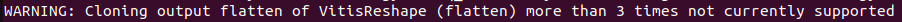
\includegraphics[scale=0.45]{Figures/hls4ml/warning_reuse_of_variable.png}
    \caption{Message d'avertissement lorsqu'une variable issue d'une couche "flatten" est réutilisée plus de $3$ fois.}
    \label{fig:warning_reuse_of_variable}
\end{figure}

La quatrième et dernière limitation rencontrée et déjà abordée dans la sous-section \ref{subsec:yolov8_utilization} concerne le déroulement des couches dans des modèles imbriqués. Cependant, il semblerait que cette limitation ait été corrigée dans une mise à jour du 16 novembre 2023 \cite{noauthor_release_nodate}.

Par ailleurs, des limitations non directement liées à \acrshort{hls4ml}, mais à la quantité de mémoire comme expliqué dans la sous-section \ref{subsec:r18_synthetize_with_hls4ml} sont également à prendre en compte.

\section{Développer et synthétiser un modèle de machine learning}

Lors de la réalisation de ce travail, nous avons commencé par prendre en main l'outil en recherchant de la documentation sur le site officiel \cite{noauthor_extension_nodate} et nous avons suivi un "tutoriel" \acrshort{hls4ml} sur comment synthétiser des réseaux neuronaux convolutifs \cite{noauthor_hls4ml-tutorialpart6_cnnsipynb_nodate}.

Bien qu'intéressants et utiles, nous avons constaté un certain manque d'informations regroupées afin de faciliter la prise en main et le développement de modèles avec l'outil. À titre d'exemple, la liste des couches supportées par \acrshort{hls4ml} a été extraite de leur code, car elle n'était pas à jour sur leur site, la limitation du nombre de réutilisations d'une variable n'a été découverte qu'au moment de la synthèse, l'utilisation d'un stride dans la couche "MaxPooling2d" déclenche une erreur même si cette dernière est censée être supportée, etc.

Ainsi, au fil du développement, nous sommes passés plusieurs fois par différentes étapes clefs pour obtenir un résultat. À partir de ces dernières, nous avons réalisé le logigramme de la figure \ref{fig:synthetize_model_with_hls4ml} présentant comment réaliser un projet de ce type à partir de zéro afin de permettre à toute personne souhaitant synthétiser son propre réseau de neurones avec \acrshort{hls4ml} de visualiser les actions à mener.\\

En parcourant celui-ci, nous commençons par développer ou tout simplement choisir le modèle désiré.

Puis, nous nous assurons que toutes les couches de ce dernier soient supportées par \acrshort{hls4ml}. Si cela n'est pas le cas, il faut vérifier si le modèle peut être adapté. Cela englobe : est-ce qu'il est possible de remplacer les couches non supportées par d'autres ? Est-ce qu'il est possible de développer soit même le code pour la couche en question ? Tout en prenant en compte les ressources nécessaires et l'impact sur le modèle de certains changements. Si cela n'est pas possible, le modèle ne peut pas être synthétisé avec \acrshort{hls4ml}. Dans le cas contraire, nous pouvons redévelopper notre modèle puis passer à la suite.

L'étape suivante n'est pas obligatoire en tant que telle pour synthétiser le modèle, mais l'inclure dans le développement permet d'obtenir un résultat plus proche de l'implémentation finale et utilisant moins de ressources.

Lorsque le réseau de neurones semble prêt à être synthétisé, nous pouvons commencer par définir la configuration de \acrshort{hls4ml}. Il faut y indiquer plusieurs informations, comme : le modèle de \acrshort{fpga} utilisé, le "reuse factor", la stratégie à adopter, la précision, etc.

Nous pouvons à présent synthétiser notre modèle. L'outil va travailler puis générer une sortie. À ce moment là nous savons si \acrshort{hls4ml} a réussi la synthèse ou non. Dans le cas où cela a été un échec, nous pouvons retrouver les erreurs rencontrées et les analyser. Nous avons retenu deux cas, les erreurs provoquées par la configuration \acrshort{hls4ml}, et celles liées au modèle. Dans le premier cas, il suffit d'adapter la configuration, et dans le second il est nécessaire de repasser par une phase d'analyse de l'erreur et d'évaluer si le modèle peut être adapté.

Finalement, si le modèle a été synthétisé avec succès, il nous est possible d'accéder au rapport de synthèse. Celui-ci nous permet d'analyser les ressources utilisées, la latence, ou encore l'\acrfull{ii}, et de modifier la configuration si le résultat n'est pas satisfaisant, par exemple : trop de ressources utilisées, une latence trop élevée, etc., jusqu'à obtenir un résultat qui nous convienne.

Une contrainte externe, déjà abordée dans la sous-section \ref{subsec:r18_synthetize_with_hls4ml}, peut venir affecter le logigramme décrit. Il s'agit de la mémoire vive utilisée. En effet, la taille du modèle et la configuration de \acrshort{hls4ml} vont venir impacter cette dernière. Il est alors nécessaire de soit modifier la configuration, soit diminuer la taille du modèle, ou le cas échéant d'utiliser une machine avec plus de ressources.\\

Comme nous venons de le voir, synthétiser un modèle avec \acrshort{hls4ml} impose des contraintes dès son développement. En prenant en compte celles-ci et les limitations de l'outil, il est alors possible d'en tirer toute la puissance.

\begin{figure}[hbt!]
    \centering
    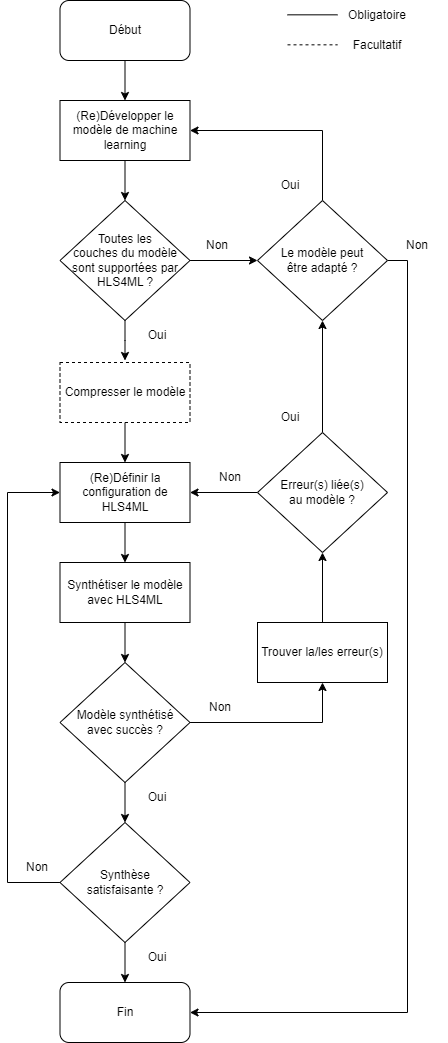
\includegraphics[scale=0.56]{Figures/hls4ml/synthetize_model_with_hls4ml.png}
    \caption{Logigramme de développement d'un modèle de machine learning et de synthèse avec \acrshort{hls4ml}.}
    \label{fig:synthetize_model_with_hls4ml}
\end{figure}

%----------------------------------------------------------------------------------------

% ModelEvaluation

\chapter{Évaluation des modèles} % Main chapter title

\label{ModelEvaluation} % For referencing the chapter elsewhere, use \ref{ModelEvaluation} 

%----------------------------------------------------------------------------------------

Dans les chapitres "Réseaux de neurones utilisés" (\ref{UsedModels}) et "Résultats" (\ref{Results}), nous allons aborder différentes métriques pour évaluer nos modèles. Afin de comprendre ce qu'elles signifient et comment elles ont été calculées, nous allons les détailler dans les sections suivantes.

\section{Intersection sur union}
\label{sec:iou}

L'intersection sur union (\acrfull{iou} en anglais) \cite{subramanyam_iouintersection_2021} est une métrique très utile pour évaluer la précision d'une prédiction par rapport à sa réalité. Celle-ci s'applique notamment aux tâches de détection et de segmentation.

Nous pouvons expliquer ce concept intuitivement avec la figure \ref{fig:iou_prediction_and_ground_truth}, où le carré rouge correspond à la prédiction réalisée, tandis que le carré vert correspond à la délimitation du panneau "STOP". 

\begin{figure}[hbt!]
    \centering
    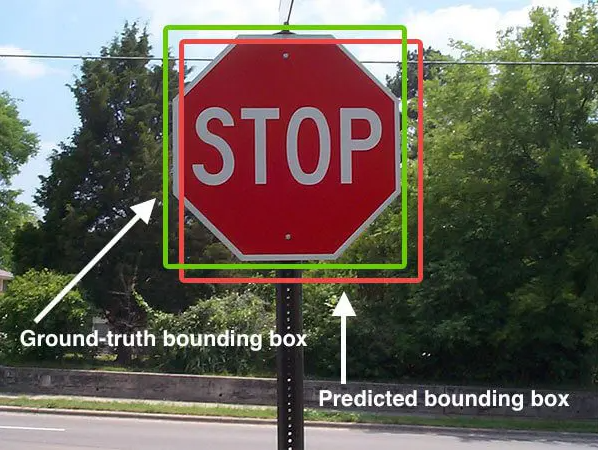
\includegraphics[scale=0.5]{Figures/model_evaluation/iou_prediction_and_ground_truth.png}
    \caption{Représentation de la formule de l'intersection sur union \cite{noauthor_jaccard_2023}.}
    \label{fig:iou_prediction_and_ground_truth}
\end{figure}

Comme son nom l'indique, l'\acrshort{iou} est définie par l'intersection, la zone qui se chevauche entre la boîte prédite et celle de référence, sur l'union, la zone couverte par les deux boîtes, comme nous pouvons le voir sur la figure \ref{fig:iou_formula}.

\begin{figure}[hbt!]
    \centering
    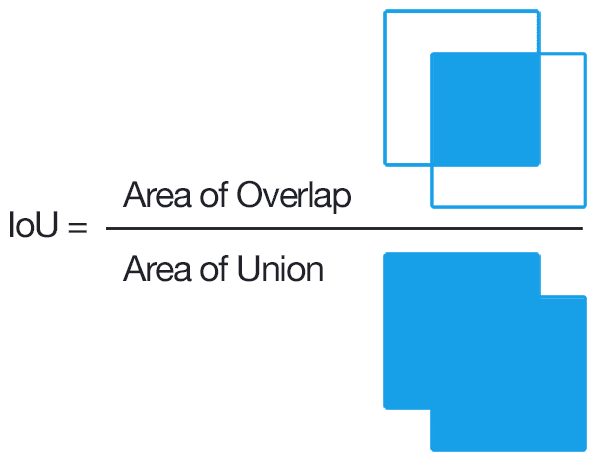
\includegraphics[scale=0.5]{Figures/model_evaluation/iou_formula.png}
    \caption{Représentation de la formule de l'intersection sur union \cite{noauthor_jaccard_2023}.}
    \label{fig:iou_formula}
\end{figure}

\break

Celle-ci est formellement décrite par la formule :

\[IoU=\frac{Aire \: de \: chevauchement}{Aire \: d'union}\]

Le résultat de ce cette opération est un nombre entre $0$ et $1$, où $0$ correspond à aucun chevauchement, et $1$ indique un chevauchement parfait.

Il peut être utilisé comme seuil pour déterminer si une prédiction est juste ou non. Dans notre travail, nous considérons une détection comme correcte si celle obtiens au moins $0.5$ de \acrshort{iou}. Cette valeur est très couramment utilisée, car elle offre un bon compromis entre la précision et la tolérance, de plus des compétitions comme The PASCAL Visual Object Classes (VOC) Challenge \cite{everingham_pascal_2010} en ont fait le seuil à adopter. Cependant, il est possible de l'adapter en fonction du projet.

\section{Matrice de confusion}

Une matrice de confusion est un outil qui permet de visualiser les performances d'un algorithme, notamment dans le domaine de l'apprentissage supervisé \cite{karimi_confusion_2021}.

Bien que nous ne l'utilisons pas directement dans nos résultats, nous utilisons plusieurs métriques issues de cette dernière que nous détaillerons dans leurs sous-sections respectives.

Celle-ci peut-être représentée sous la forme d'une matrice à deux dimensions comme sur la table \ref{tab:confusion_matrix}, où dans notre cas, la première correspond aux éléments réels, et la seconde aux prédictions de nos modèles.

\begin{table}[!ht]
    \caption{Représentation d'une matrice de confusion}
    \label{tab:confusion_matrix}
    \centering
    \begin{tabular}{|c|c|c|c|  }
        \hhline{----}
        \multicolumn{2}{|c|}{} & \multicolumn{2}{c|}{\cellcolor{gray!50} Prédit}\\
        \hhline{~~--}
        \multicolumn{2}{|c|}{} & \cellcolor{gray!25}Positif & \cellcolor{gray!25}Négatif\\
        \hhline{----}
        \cellcolor{gray!50} & \cellcolor{gray!25}Positif & Vrai positif & Faux négatif\\
        \arrayrulecolor{gray!50}
        \cline{1-1}
        \arrayrulecolor{black}
        \hhline{~---}
        \multirow{-2}{*}{\cellcolor{gray!50} Réel} & \cellcolor{gray!25}Négatif & Faux positif & Vrai négatif\\
        \hline
    \end{tabular}
\end{table}

\break

\subsection{Vrais / Faux - positifs / négatifs}

Lorsqu'une prédiction est réalisée, celle-ci va être placée dans la matrice de confusion. 
Comme nous pouvons l'observer sur la table \ref{tab:confusion_matrix}, cette dernière est composée de quatre catégories :\\

\begin{itemize}
    \item \textbf{Vrai positif} : La prédiction est correcte.
    \item \textbf{Faux positif} : La prédiction est fausse.
    \item \textbf{Faux négatif} : Un élément réel qui n'a pas été prédit.
    \item \textbf{Vrai négatif} : Ne s'applique pas dans notre cas. Cependant, il s'agirait d'aucune détection où il n'y a rien à détecter. Or, dans les problèmes de détection d'objets, il y a un grand nombre de zones sur une image qui ne doivent pas être détectées, et les vrais négatifs correspondraient à toutes ces zones correctement non détectées. Ainsi, nous n'utiliserons aucune métrique la nécessitant, et la valeur de ce cas sera nulle.\\
\end{itemize}

Comme nous venons de le voir, les détections à elles seules ne suffisent pas à remplir la matrice de confusion. Il nous faut également les éléments réels de l'image que notre modèle tente de détecter. Ceux-ci nous permettront d'identifier si une détection est correcte ou non, en utilisant par exemple l'\acrshort{iou}, et de compléter notre table lorsque toutes les détections auront été traitées, s'il reste des éléments réels qui n'ont pas été détectés.\\

À ce stade, à l'aide de notre matrice de confusion, nous pouvons déjà constater la capacité d'un modèle à réaliser des détections correctes, et observer si celui-ci a une tendance (ou non) à prédire trop de faux positifs, ou au contraire à réaliser trop des faux négatifs. De telles informations se révèlent très utiles pour affiner certains seuils utilisés comme le score de confidence minimum pour prendre en compte une détection, mais aussi comment les résultats se comportent avec un l'\acrshort{iou} plus élevé. Ceux-ci devront être adaptés en fonction des applications et des tolérances.

À partir de ces données, nous allons pouvoir calculer une partie des métriques que nous utilisons et analysons dans le chapitre résultats (\ref{Results}), afin de mieux comprendre le comportement du modèle utilisé.

\subsection{Précision}

La précision correspond à la proportion d'éléments corrects parmi tous ceux prédits par le modèle. Elle est décrite par la formule suivante :

\[pr\acute{e}cision = \frac{vrais \: positifs}{vrais \: positifs + faux \: positifs}\]

Celle-ci permet donc d'évaluer la capacité du modèle à réaliser des prédictions correctes. Cependant, il est nécessaire de l'associer à d'autres métriques comme le rappel. En effet, en utilisant uniquement les vrais positifs et les faux positifs, la précision n'est pas sensible aux faux négatifs. Ainsi, il est très probable d'obtenir un résultat de $100\%$ en ne sélectionnant que quelques éléments détectés pour lesquels le modèle possède un score de confiance très élevé. En contrepartie, il est très probable que ce dernier n'ait pas détecté tous les éléments réels, mais cela n'apparaît pas dans cette métrique.

\subsection{Rappel}

Le rappel correspond à la proportion d'éléments prédits correctement parmi tous les éléments réels à prédire. Il est décrit par la formule suivante :

\[rappel = \frac{vrais \: positifs}{vrais \: positifs + faux \: n\acute{e}gatifs}\]

Celui-ci permet d'évaluer la capacité du modèle à détecter les éléments attendus. Tout comme pour la précision, il est nécessaire d'associer le rappel à d'autres métriques comme à cette dernière par exemple. Effectivement, à présent nous utilisons les vrais positifs et faux négatifs, rendant le rappel insensible aux faux positifs. En acceptant toutes les prédictions de notre modèle, même celles pour lesquelles le score de confiance du modèle est nul, nous pourrions alors obtenir un score de rappel très élevé au détriment de la précision.

\subsection{Courbe précision rappel}

La courbe précision rappel permet, comme son nom l'indique, de visualiser l'évolution de la précision en fonction du rappel pour le modèle évalué. Celle-ci est tracée en diminuant progressivement le seuil du score de confiance des prédictions réalisées. De plus, dans le cadre de la détection d'objets, l'\acrshort{iou} est également utilisé afin définir si une prédiction est correcte ou non.\\

La courbe parfaite, comme illustrée par la figure \ref{fig:perfect_precision_recall_curve}, est une courbe pour laquelle peut importe le rappel, la précision reste à $1$. Cela signifie que le modèle évalué est capable de détecter tous les éléments réels sans faire d'erreurs.

\begin{figure}[hbt!]
    \centering
    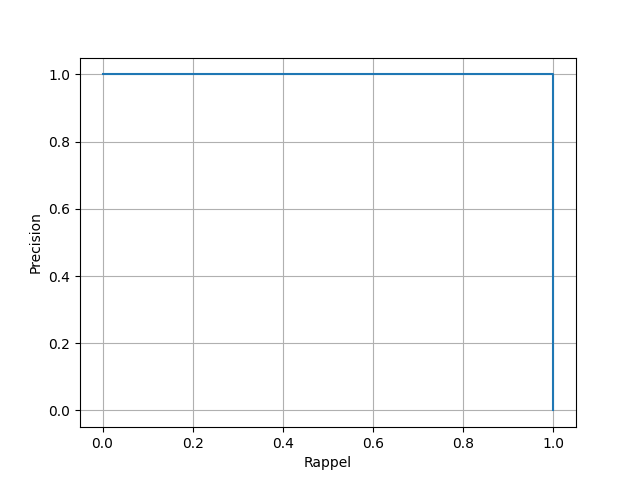
\includegraphics[scale=0.7]{Figures/model_evaluation/perfect_precision_recall_curve.png}
    \caption{Courbe précision rappel parfaite}
    \label{fig:perfect_precision_recall_curve}
\end{figure}

\break

Ainsi, lorsqu'une courbe adopte un tracé haut et vers la droite, qui tend vers cette courbe idéale, celle-ci nous indique que le modèle performe bien. Il possède alors une précision élevée pour un rappel élevé, et il détecte correctement la plupart des éléments tout en minimisant les faux positifs.

Inversement, une courbe basse et vers la gauche indique que le modèle possède de piètres performances.

\subsection{Average precision et mean average precision}

L'\acrfull{ap} (précision moyenne en français) correspond à l'aire sous la courbe précision rappel \cite{padilla_rafaelpadillaobject-detection-metrics_2024}. Celle-ci permet d'évaluer les performances d'un modèle sans fixer de seuil pour le score de confiance, et par conséquent, d'obtenir une mesure unique combinant à la fois la précision et le rappel pour un seuil d'\acrshort{iou} donné.

Cette dernière est calculée à l'aide de la formule suivante :

\[\acrfull{ap} = \int_{0}^{1} p(r)dr\]

Où la fonction $p(r)$ correspond à la courbe précision rappel précédemment calculée.\\

Cette mesure est liée à une classe et doit être recalculée pour toutes les classes prédites par le modèle. À partir des différents \acrshort{ap}, il est alors possible de calculer la \acrfull{map} (la moyenne de la précision moyenne) à l'aide de la formule :

\[\acrfull{map}=\frac{1}{k}\sum_{i=0}^{k}AP_i\]

Où $k$ correspond au nombre de classes, et $AP_i$ l'\acrshort{ap} pour la classe $i$.

Dans notre cas, comme nous ne travaillons qu'avec une classe, l'\acrshort{ap} et la \acrshort{map} sont identiques.

Comme souligné plus tôt, le résultat obtenu est celui pour un \acrshort{iou} donné. Nous avons également déjà abordé dans sa section (\ref{sec:iou}) que celui-ci est généralement égal à $0.5$. Nous pouvons donc faire varier cette valeur pour observer l'évolution de l'\acrshort{ap} à différents seuils. Cependant, il reste complexe et arbitraire de choisir d'autres valeurs de seuil. Ainsi, nous avons décidé d'utiliser la métrique principale d'évaluation utilisée par \acrshort{coco}, c'est-à-dire l'\acrshort{ap} à un \acrshort{iou} de $.5:.05:.95$ \cite{noauthor_coco_nodate}. Cela signifie que nous calculons l'\acrshort{ap} pour les \acrshort{iou} en commençant à $0.5$ jusqu'à $0.95$ avec un pas de $0.05$, puis nous réalisons la moyenne de tous les \acrshort{ap} obtenus.

Cette fois-ci non seulement nous obtenons un résultat qui n'est pas sensible au seuil de confiance, mais nous obtenons également une valeur qui prend en compte la capacité du modèle à effectuer des détections de plus en plus précises.

\subsection{Score F1}

La dernière métrique utilisée est le score F1. Il s'agit de la moyenne harmonique de la précision et du rappel, nous permettant d'évaluer la performance du modèle. Il est décrit par la formule suivante :

\[score \: F_1 = 2 \cdot \frac{pr\acute{e}cision \cdot rappel}{pr\acute{e}cision + rappel} = \frac{2 \cdot vrais \: positifs}{2 \cdot vrais \: positifs + faux \: positifs + faux \: n\acute{e}gatifs}\]

Ce rapport s'avère précieux et complémentaire pour observer la qualité des prédictions réalisées dans un contexte où la précision et le rappel sont les deux très importants. Un score de $1$ signifierait que toutes les détections traitées étaient correctes et qu'elles couvraient l'ensemble des éléments à détecter. Un score F1 proche de $1$ indique des performances élevées, au contraire d'un résultat autour de $0.5$ indiquant que le modèle à des difficultés avec la précision, le rappel, ou les deux.


%----------------------------------------------------------------------------------------

% UsedModels
\chapter{Réseaux de neurones utilisés} % Main chapter title
\label{UsedModels} % For referencing the chapter elsewhere, use \ref{UsedModels} 

%----------------------------------------------------------------------------------------

\section{Réseau de neurones}
\label{sec:nn}

Avant d'aborder les réseaux de neurones utilisés dans ce travail, nous allons débuter en détaillant les notions de base nécessaires à leur compréhension.

\subsection{Perceptron}
\label{sec:perceptron}

Le modèle d'apprentissage supervisé le plus simple est le perceptron. Il s'agit simplement d'un neurone reproduisant le comportement simplifié d'un neurone biologique. Il possède des entrées et une sortie, ainsi qu'un poids associé à chaque entrée ayant pour but de reproduire l'excitation ou l'inhibition des synapses \cite{fleuret_deep_nodate-4}.

Le neurone va simplement recevoir en entrée une ou plusieurs valeurs, qui vont être pondérées par un poids donné. Il effectuera la somme de ces dernières, à laquelle un biais est ajouté. Puis cette somme sera passée dans une \hyperref[sec:fa]{fonction d'activation} qui nous donnera le résultat en sortie.

Formellement, le neurone est défini par la formule mathématique suivante :

\[f(x)=\sigma(b+\sum_{j=1}^{p}w_j \cdot x_j)\]

Où $x$ correspond à l'entrée $j$, $w$ au poids $j$, $b$ au biais, et $\sigma$ à la fonction d'activation. Cette dernière est généralement non linéaire, et elle est toujours appliquée en sortie. Le choix de la fonction d'activation dépend des besoins du modèle. Voici un exemple simple assignant à 1 toutes les valeurs supérieures ou égales à 0 et à 0 toutes les valeurs négatives :

\[\sigma(x)= \begin{cases}
    1 \text{ si } x \geq 0\\
    0 \text{ sinon}
    \end{cases}
\]

Dans le cas ci-dessus, avec les poids adéquats, notre perceptron serait capable de séparer différentes entrées $x$ entre deux classes. Il fonctionnerait donc en tant que classifieur binaire.

Par ailleurs, l'entrée $x$ de notre perceptron peut être une simple valeur, mais aussi un vecteur. Il en va de même pour les poids $w$. La figure \ref{fig:neurone_formel} permet de visualiser comment un perceptron est composé notamment lorsqu'il a plusieurs entrées.

\begin{figure}[htb!]
    \centering
    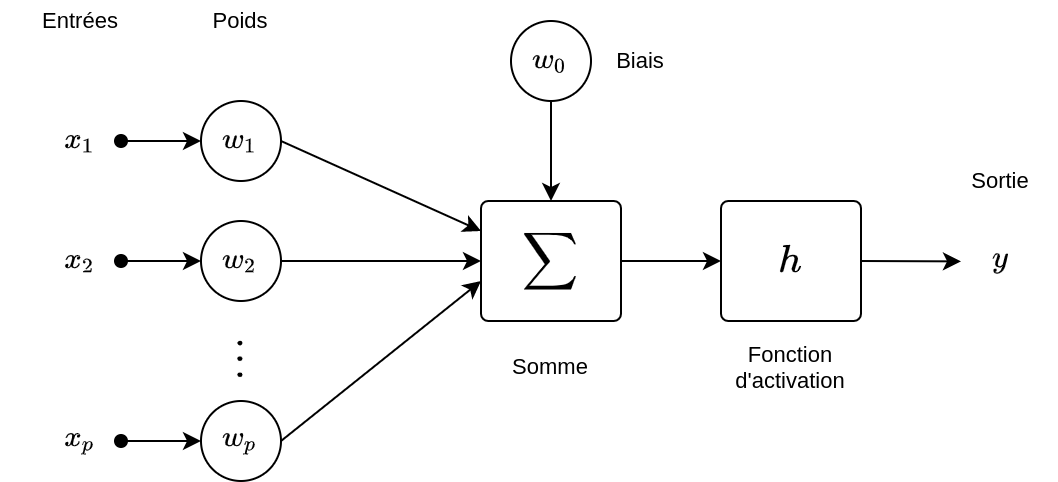
\includegraphics[scale=0.30]{Figures/neurone_formel_representation.png}
    \caption{Perceptron de $p$ entrées \cite{noauthor_perceptron_3png_nodate}.}
    \label{fig:neurone_formel}
\end{figure}

\pagebreak

Un perceptron peut également proposer plusieurs sorties. Pour cela, le vecteur de poids augmente ses dimensions aux nombres de sorties et le biais devient un vecteur. Toutes les entrées vont donc être connectées à ces sorties, et multipliées par les poids correspondants. La figure \ref{fig:perceptron_multi_output} illustre la composition d'un perceptron possédant deux sorties. 

\begin{figure}[hbt!]
    \centering
    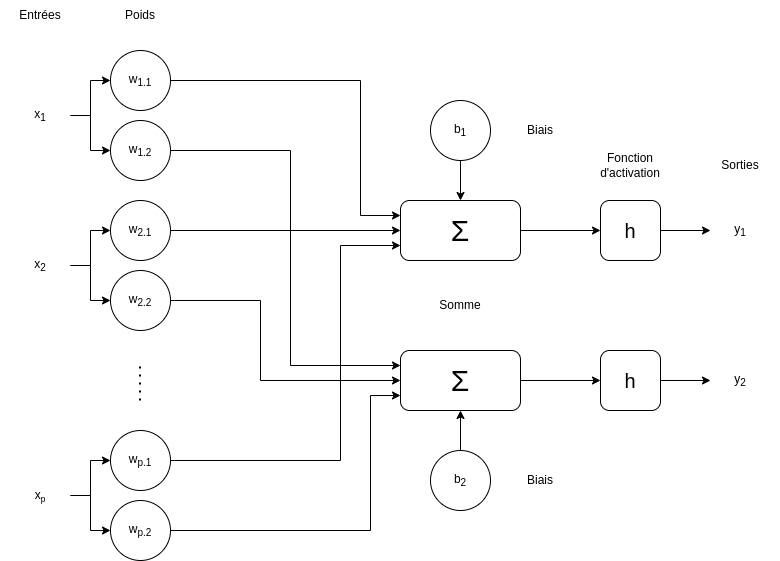
\includegraphics[scale=0.50]{Figures/perceptron_multi_sortie.png}
    \caption{Perceptron de $p$ entrées avec deux sorties.}
    \label{fig:perceptron_multi_output}
\end{figure}

Cette structure relativement simple peut être complexifiée en ajoutant des couches entre l'entrée et la sortie. Une couche correspond à une structure définie, dans notre cas à un autre perceptron. Il s'agit alors d'un perceptron multicouche, un type de réseau de neurones. Celui-ci est caractérisé par le fait qu'il possède une couche d'entrée, au moins une couche cachée, et une couche de sortie. Sur la figure \ref{fig:perceptron_multicouche}, nous pouvons voir comment est composé un perceptron multicouche entièrement connecté. Il est nommé ainsi, car chaque neurone d'une couche est connecté à tous les neurones de la couche suivante.

\begin{figure}[hbt!]
    \centering
    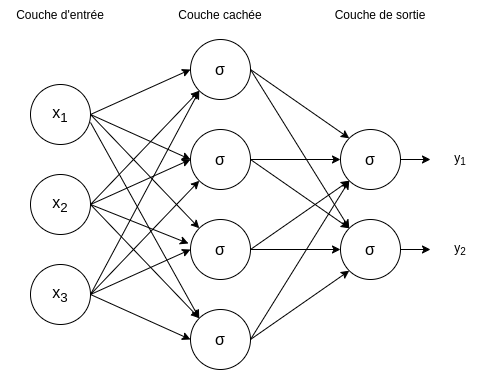
\includegraphics[scale=0.50]{Figures/perceptron_multicouche.png}
    \caption{Perceptron multicouche.}
    \label{fig:perceptron_multicouche}
\end{figure}

\subsection{Apprentissage}

Comme nous avons vu précédemment, un modèle est capable d'effectuer des tâches données, comme une classification binaire, lorsqu'il possède les poids et biais adéquats. Dans le cadre du machine learning, ces derniers ne sont pas connus par avance, et varient en fonction du problème. Il est donc nécessaire que le modèle passe par une phase d'apprentissage ou celui-ci va s'entraîner afin de définir les paramètres les plus adaptés. Ce sont donc ceux-ci qui vont évoluer jusqu'à ce qu'ils permettent d'obtenir, si cela est possible, la/les sorties escomptées \cite{fleuret_deep_nodate-3}.

Il existe différents types d'apprentissages, cependant, dans le cadre de ce travail, nous allons aborder le cas de l'apprentissage supervisé qui correspond à notre cas. En effet, ce type d'apprentissage est défini par des classes prédéterminées et des exemples connus qui sont étiquetés.

L'entraînement du modèle se divise en deux parties. La première consiste à effectuer toutes les opérations définies par notre réseau de neurones sur les entrées d'entraînement. Ces entrées sont divisées en lots, ou "batchs" en anglais, qui définissent le nombre d'échantillons avec lesquels le modèle va travailler avant de mettre à jour les paramètres. Cette phase est communément appelée "forward pass" ou propagation avant en français.

La deuxième va réaliser l'inverse, c'est-à-dire une propagation arrière "backward pass". Le but de cette partie est de rétropropager l'erreur depuis la sortie vers l'entrée, et de mettre à jour les paramètres du modèle, grâce un algorithme d'optimisation, afin de minimiser l'erreur lors des prochaines itérations.

L'erreur utilisée par la backward pass est calculée en évaluant le résultat en sortie du modèle avec la sortie attendue. Cette évaluation est réalisée grâce à une fonction de coût qui varie suivant le problème à traiter. Dans ce travail par exemple, la fonction coût \acrfull{mse} est utilisée. Celle-ci est définie comme suit :

\[\acrshort{mse}=\frac{1}{n}\sum^{n}_{i=1} (Y_i-\hat{Y}_i)^{2}\]

Où $n$ est le nombre de prédictions, $Y$ est le vecteur correspondant aux valeurs à prédire, $\hat{Y}$ est le vecteur contenant les valeurs prédites. Comme le nom de cette fonction le laisse deviner, celle-ci calcule la moyenne de l'erreur au carré, pour laquelle l'erreur correspond simplement à la différence entre la valeur à prédire et la valeur prédite.

Lors de la rétropropagation de l'erreur, il est nécessaire de mettre à jour les paramètres. Pour ce faire, il faut utiliser un algorithme d'optimisation. Il en existe plusieurs, néanmoins, nous allons nous baser sur la descente de gradient pour les explications à suivre. En effet, ce dernier est très connu, et permet de trouver un minimum local en allant, à chaque itération, dans la direction opposée au gradient de la fonction à partir du point courant.

Afin de modifier les paramètres de sorte qu'ils minimisent l'erreur, nous devons donc calculer leur gradient. Pour trouver celui-ci, il faut calculer la dérivée de la fonction de coût par rapport aux paramètres. La mise à jour de la valeur des poids, représentés ici par $w^{(l)}$, est formellement décrite par la formule :

\[w^{(l)}=w^{(l)}-\eta{}\frac{\partial{}\ell}{\partial{}w^{(l)}}\]

Et pour les biais représentés par $b^{(l)}$ :

\[b^{(l)}=b^{(l)}-\eta{}\frac{\partial{}\ell}{\partial{}b^{(l)}}\]

Dans ces formules, nous pouvons voir apparaître le symbole $\eta$ qui correspond au taux d'apprentissage. Celui-ci a un impact direct sur l'apprentissage. En effet, lorsque $\eta$ est élevé la valeur des paramètres sera également modifiée par une valeur plus importante. Cela implique, notamment au début de l'entraînement, que les paramètres vont rapidement converger vers la solution minimisant la fonction de coût. Or, à partir d'un moment, si $\eta$ est trop élevé, la valeur des paramètres va osciller autour de la solution minimisant la fonction de coût sans pouvoir l'atteindre. Inversement, lorsque $\eta$ est faible, il faudra plus de temps aux paramètres pour converger vers la solution minimisant la fonction de coût, sans parler du risque de rester piéger dans un minimum local. Nous pouvons observer ces principes sur la figure \ref{fig:learning_rate_choice}.

\begin{figure}[hbt!]
    \centering
    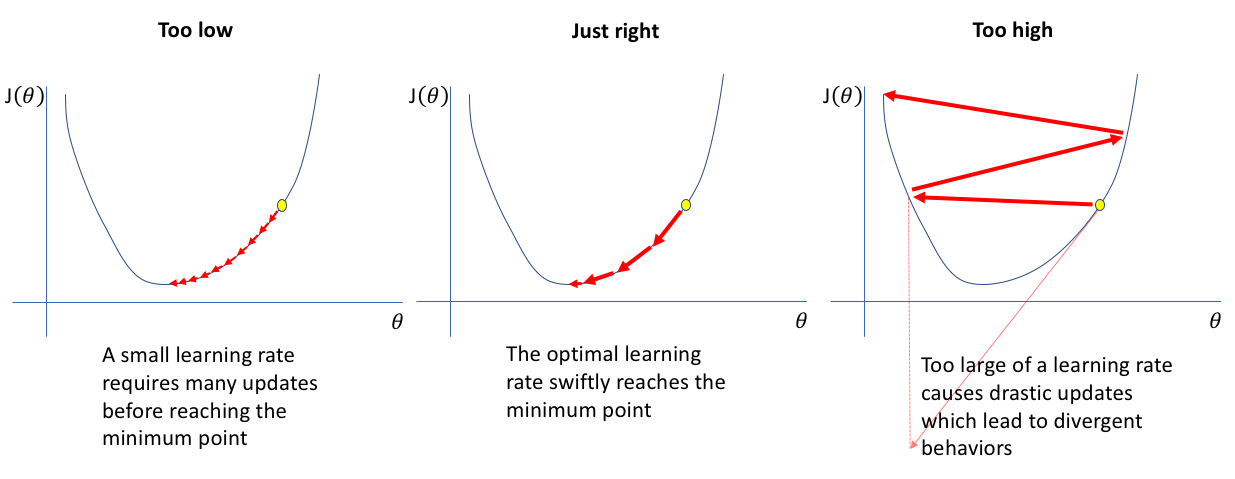
\includegraphics[scale=0.3]{Figures/learning_rate_choice.png}
    \caption{Impact du taux d'apprentissage sur l'entraînement \cite{noauthor_learning_rate_choicepng_nodate}.}
    \label{fig:learning_rate_choice}
\end{figure}

Comme nous avons pu le voir, lors de l'entraînement le modèle va mettre à jour ses poids après chaque batchs. Lorsque celui-ci a parcouru tous les batchs contenant l'ensemble des données d'entraînement, le réseau de neurones vient de réaliser une époque (epoch en anglais). Cependant, même si le jeu de données prévu est conséquent, il est nécessaire que le modèle itère sur plusieurs époques afin d'être bien entraîné. Ce nombre n'est pas connu à l'avance. S'il est trop faible, le réseau de neurones risque de ne pas bien performer et ne pourra pas généraliser ce qu'il a appris à de nouvelles entrées. Ce phénomène est appelé sous-apprentissage (underfitting en anglais).

Inversement, si le nombre d'époques est trop élevé, le modèle sera trop entraîné sur les données d'entraînement ce qui aura pour effet d'obtenir d'excellentes performances sur l'ensemble d'entraînement, mais le réseau de neurones ne sera pas capable de généraliser. Le modèle obtiendra donc de pauvres performances sur de nouvelles entrées. Ce fait se nomme surapprentissage (overfitting en anglais).

C'est pour les deux raisons précédentes qu'il est nécessaire de visualiser l'évolution de l'erreur tout au long de l'entraînement pour les données d'entraînement et de validation. Il également important de tester les performances de notre modèle sur un jeu de données qui n'est pas utilisé. Cela nous donne des informations cruciales sur l'évolution de notre réseau de neurones. Nous pouvons par exemple voir ; lorsque l'erreur ne diminue plus, lorsque l'erreur des données de validation augmente alors que celle des données d'entraînement diminue, mais également lorsque le modèle commence à performer moins bien sur notre jeu de données de test. Avec ces indications, il est possible d'estimer le nombre d'époques nécessaires à notre modèle pour qu'il soit suffisamment entraîné pour généraliser sur de nouvelles entrées avec les performances recherchées, sans qu'il ait atteint le problème du surapprentissage.

\subsection{Réseau neuronal convolutif et convolution}

Les réseaux neuronaux convolutifs (\acrshort{cnn}) sont un type d'architecture de réseau de neurones utilisés notamment dans le domaine du traitement d'images \cite{fleuret_deep_nodate-1}. À la différence du perceptron multi-couche qui possède des couches de neurones entièrement connectées, les \acrshort{cnn} utilisent des couches de convolution avec des filtres adaptables qui leur permettent de capturer des motifs locaux tout en préservant leurs relations spatiales, et d'apprendre les caractéristiques de l'entrée. C'est à ce type de réseau de neurones qu'appartiennent les modèles utilisés dans ce travail.\\

L'idée derrière une couche de convolution est qu'elle va appliquer la même transformation linéaire locale à l'ensemble de l'entrée. Ainsi, lorsqu'une transformation est significative à un endroit, elle le sera partout. De plus, la convolution préserve la structure du signal, c'est-à-dire qu'une entrée de dimensions $n$ va conserver ses dimensions en sortie, mais la taille de celle-ci peut changer.

\begin{figure}[hbt!]
    \centering
    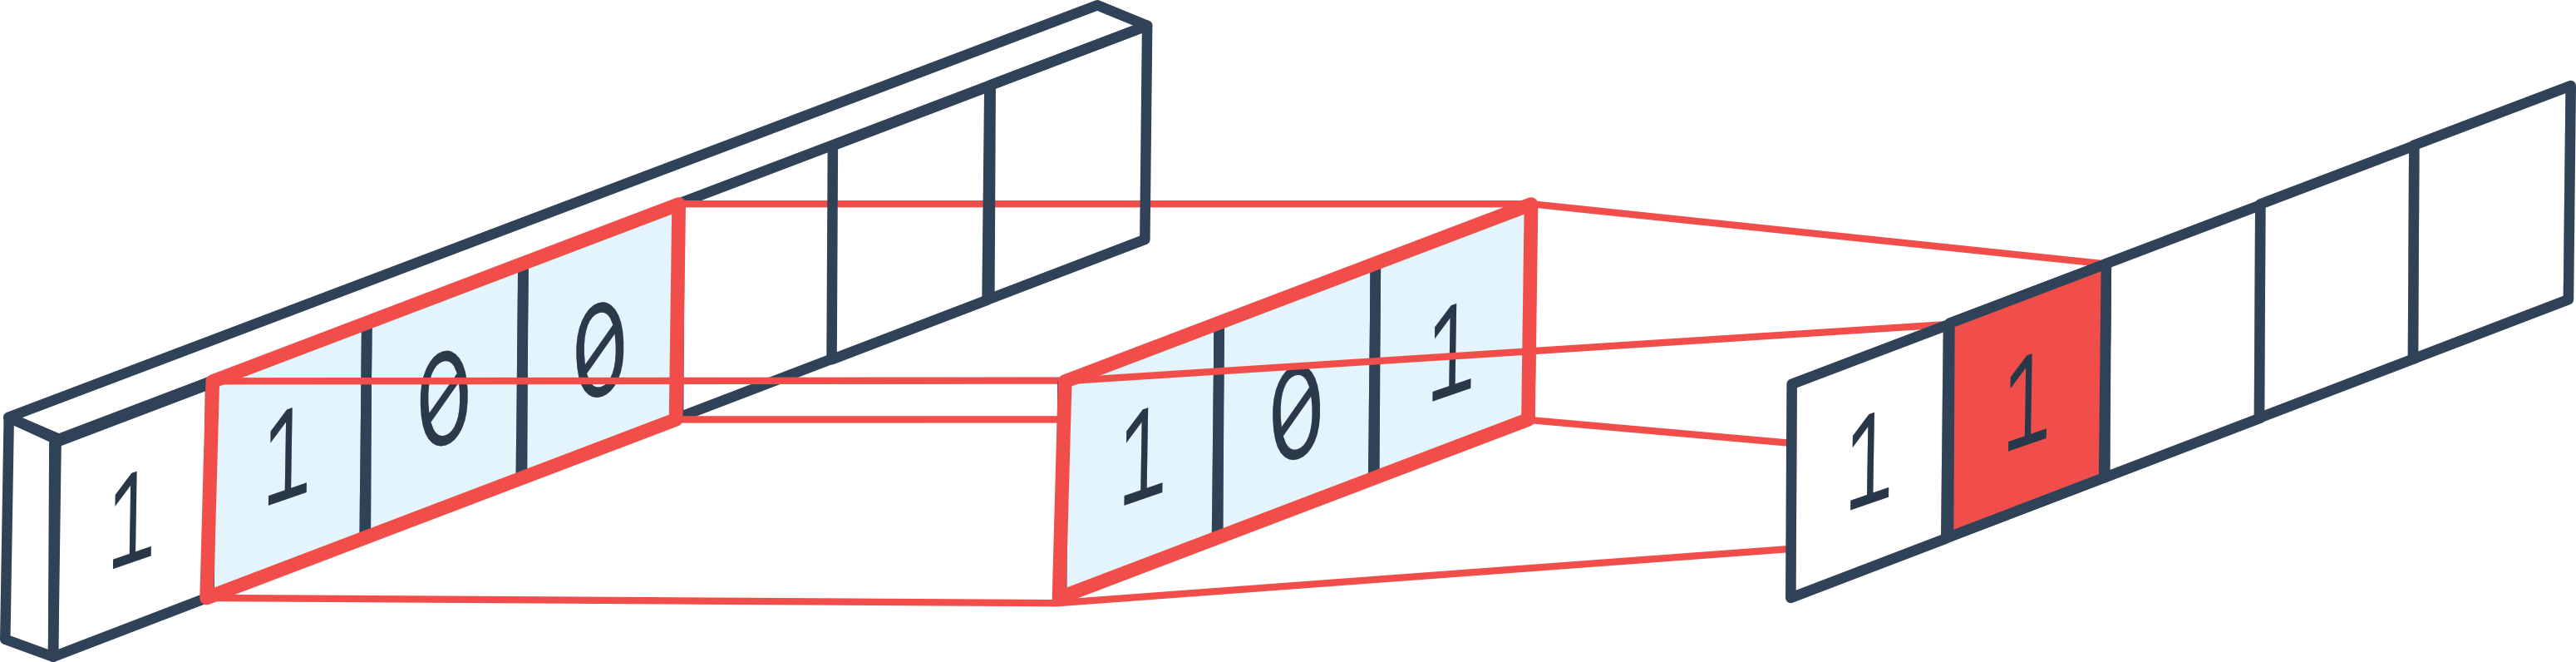
\includegraphics[scale=0.3]{Figures/convolution_exemple.png}
    \caption{Exemple 1D d'une convolution \cite{noauthor_wnixdpng_nodate}.}
    \label{fig:convolution_exemple}
\end{figure}

La convolution consiste, comme nous pouvons le voir sur la figure \ref{fig:convolution_exemple}, en un noyau de convolution, qui correspond à un vecteur de poids (aussi appelé kernel ou filtre), et qui réalise un produit scalaire sur une partie de même taille du signal en entrée. Tout comme il est possible de l'observer sur la figure \ref{fig:convolution_stride_example}, le kernel va traverser l'ensemble du signal à un pas donné qui est nommé stride.

\begin{figure}[hbt!]
    \centering
    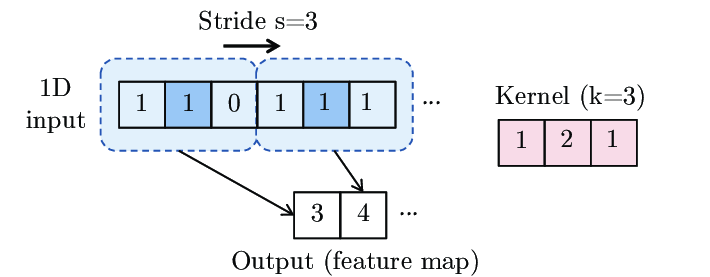
\includegraphics[scale=1.2]{Figures/convolution_stride_example.png}
    \caption{Exemple de stride sur une entrée à une dimension \cite{noauthor_figure_nodate}.}
    \label{fig:convolution_stride_example}
\end{figure}

Par défaut, le stride est de $1$, cependant, lorsque celui-ci est supérieur à $1$, il est possible que le noyau ne puisse pas couvrir l'ensemble de l'entrée et que certaines valeurs se retrouvent ignorées. Pour une entrée $x$ à une dimension de longueur $m$ et pour un kernel $w$ à une dimension de longueur $n$, la convolution au point $i$ (avec un stride de un) peut être formellement décrite comme :

\[
(x * w)_i = \sum^{n}_{j=0} x_{i+j} \cdot w_j
\]

Ce procédé implique que la sortie de notre convolution, bien que de même dimension, n'aura pas la même taille que l'entrée. Celle-ci peut être calculée à partir de la taille de l'entrée et celle de la convolution qui va être appliquée. Par exemple, dans le cas d'une image, l'entrée sera de taille $C \times H \times W$, où $C$ correspond au nombre de canaux (généralement trois, pour $RGB$), $H$ et $W$ respectivement à la hauteur et largeur. La couche de convolution aura un paramètre $D$ correspondant au nombre de kernels qui seront appliqués, et chacun aura une taille définie par $C \times h \times w$, le nombre de canaux est identique à celui de l'image. La sortie d'une telle convolution sera de taille $D \times (H - h + 1) \times (W - w + 1)$. La figure \ref{fig:image_convolution_example} illustre une convolution entre une image $RGB$ de taille $W \times H \times C$ et deux filtres de taille $w \times h \times C$.

\begin{figure}[hbt!]
    \centering
    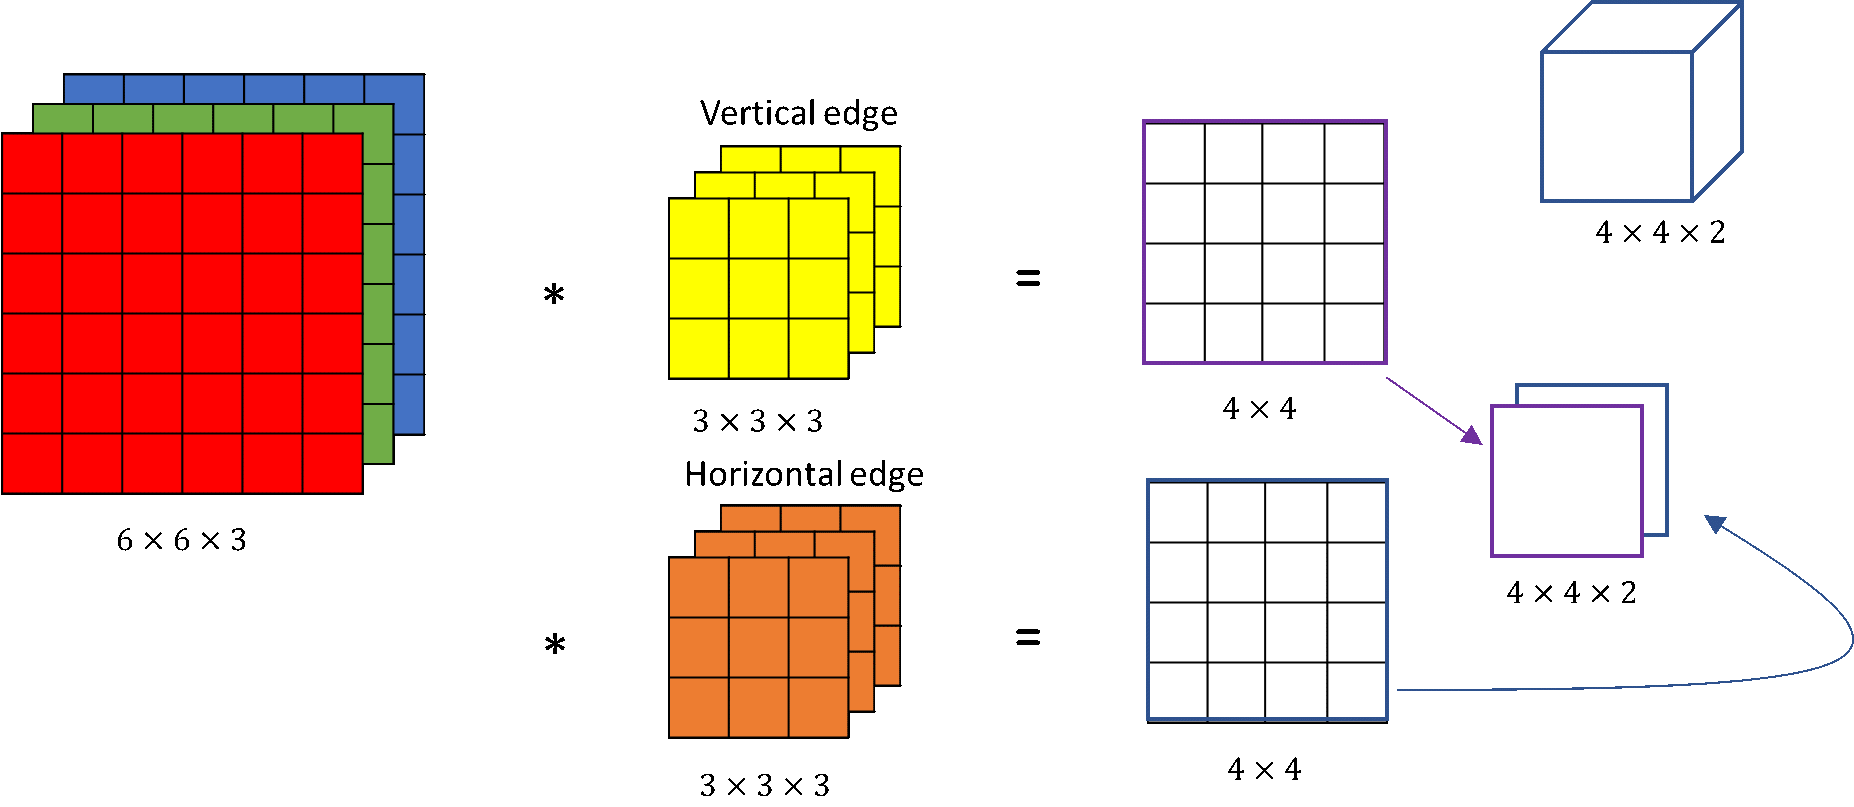
\includegraphics[scale=0.38]{Figures/image_convolution_example.png}
    \caption{Résultat d'une convolution entre une image RGB et deux filtres différents \cite{noauthor_06_09png_nodate}.}
    \label{fig:image_convolution_example}
\end{figure}

Comme vu précédemment, la taille de la sortie d'une convolution est plus petite que celle de l'entrée. Même si cela n'est pas forcément critique, lorsque plusieurs couches de convolutions s'enchaînent, cette différence va s'accroître. Ainsi, pour limiter cet effet, il est possible d'utiliser ce qui est appelé padding. Ce procédé consiste à ajouter des zéros autour de notre entrée avant d'appliquer la convolution afin de gérer la taille de la sortie. La figure \ref{fig:convolution_padding_example} montre un exemple de padding autour d'une entrée à deux dimensions.

\begin{figure}[hbt!]
    \centering
    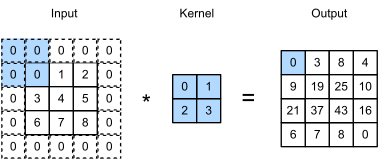
\includegraphics[scale=0.6]{Figures/convolution_padding_example.png}
    \caption{Exemple de convolution avec padding \cite{mohammed_spatiotemporal_2024} Figure 1.}
    \label{fig:convolution_padding_example}
\end{figure}

\subsection{Fonctions d'activation}
\label{sec:fa}

Comme nous avons pu le voir dans la section sur le \hyperref[sec:perceptron]{perceptron}, les fonctions d'activation font partie intégrante de la structure d'un réseau de neurones. Celles-ci sont généralement des fonctions non linéaires appliquées à la sortie d'un neurone.

Nous allons voir les différentes fonctions d'activation qui sont abordées ou utilisées dans ce travail.

Commençons par la fonction \acrfull{relu}. Celle-ci est très simple et définie par :

\[f(x)=max(0,x)\]

Et représentée visuellement par la figure \ref{fig:activation_functions_relu}.

\begin{figure}[hbt!]
    \centering
    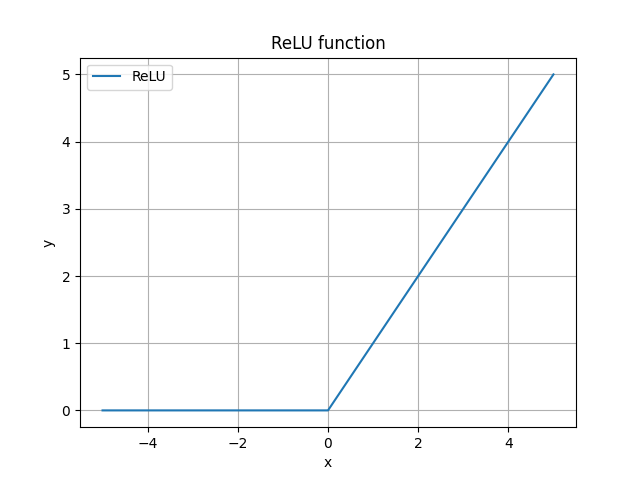
\includegraphics[scale=0.6]{Figures/activation_functions/relu.png}
    \caption{Fonction d'activation \acrshort{relu}.}
    \label{fig:activation_functions_relu}
\end{figure}

La deuxième fonction utilisée est la sigmoïde. Celle-ci est plus complexe que la \acrshort{relu}, et décrit une courbe en forme de S comme visible sur la figure \ref{fig:activation_functions_sigmoid}. Les résultats de cette fonction sont contenus dans l'intervalle $[0;1]$. Cela permet d'obtenir des valeurs similaires à des probabilités qui sont notamment utilisées dans le modèle Resnet18+Tête, décrit dans la section \ref{sec:resnet18}, pour établir le score de confiance de la prédiction réalisée par le neurone. Voici la formule la décrivant :

\[f(x)=\frac{1}{1+e^{-x}}\]

\begin{figure}[hbt!]
    \centering
    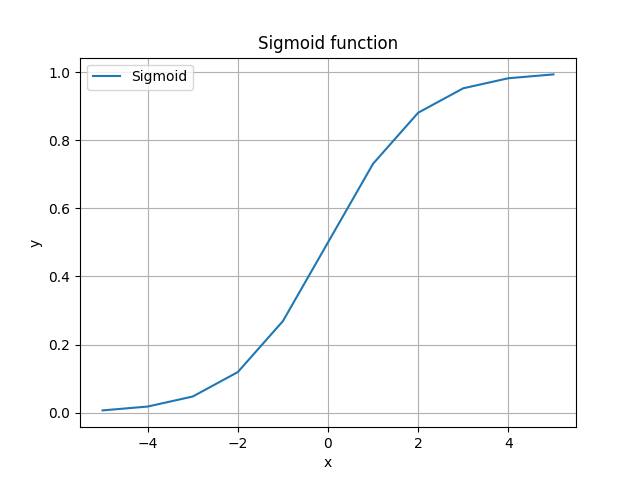
\includegraphics[scale=0.6]{Figures/activation_functions/sigmoid.png}
    \caption{Fonction d'activation sigmoïde.}
    \label{fig:activation_functions_sigmoid}
\end{figure}

La fonction \acrfull{silu} est tout comme la fonction \acrshort{relu} un redresseur. Il s'agit d'une variante qui évite que sa dérivée devienne nulle lorsque la valeur en entrée est négative. Comme il est possible de le voir sur la figure \ref{fig:activation_functions_silu} les valeurs négatives, bien que plus petites, sont toujours présentes. Cette fonction est définie par :

\[f(x)=x \cdot sigmoid(x)\]

\begin{figure}[hbt!]
    \centering
    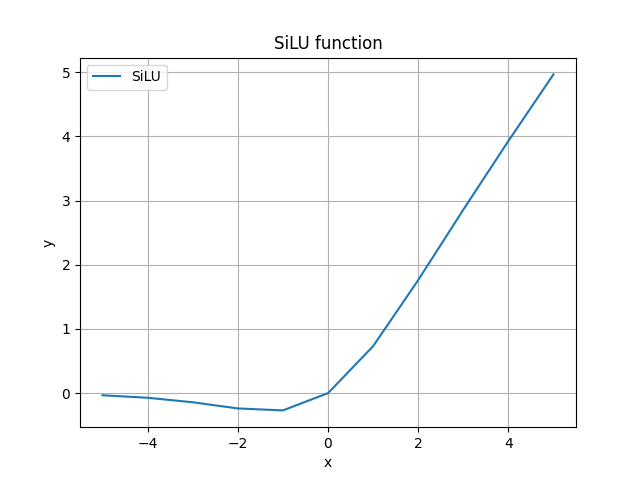
\includegraphics[scale=0.6]{Figures/activation_functions/silu.png}
    \caption{Fonction d'activation sigmoïde.}
    \label{fig:activation_functions_silu}
\end{figure}

Finalement, la fonction swish ressemble à la fonction \acrshort{silu}, à la différence qu'elle possède un paramètre $\beta$. Lorsque ce dernier est défini à 1 alors les deux fonctions sont identiques. Dans la bibliothèque Keras qui a été utilisée, la fonction swish est équivalente à la fonction \acrshort{silu}.
\newpage

\subsection{Fonction de pooling}

Le pooling est un concept important des réseaux de neurones convolutifs. Il s'agit d'une opération qui permet de diminuer la taille de l'entrée tout en préservant les caractéristiques de cette dernière \cite{fleuret_deep_nodate}. Cela permet ainsi de réduire la quantité de paramètres nécessaires dans le réseau, et par extension le nombre de calculs.

Il existe différentes fonctions de pooling, néanmoins nous allons nous concentrer sur les deux utilisées dans ce travail.

Le max-pooling est une opération de pooling qui va parcourir l'entrée par "fenêtres" d'une taille fixée par avance, et ressortir la valeur maximale de chaque zone pour générer la sortie. Sur l'entrée suivante à une dimension : $[1,2,3,4,3,2]$, pour une fenêtre de taille 3, nous aurons en sortie : $[3,4]$. En effet, nous avons appliqué notre première fenêtre de taille 3 sur l'entrée pour traiter juste la partie : $[1,2,3]$, pour laquelle nous avons retenu uniquement la valeur la plus élevée. Puis de même avec la deuxième partie de l'entrée : $[4,3,2]$.  La figure \ref{fig:maxpool_example} illustre le principe à partir d'une entrée de taille 4x4 à laquelle un max-pooling de 2x2 est appliqué.

\begin{figure}[hbt!]
    \centering
    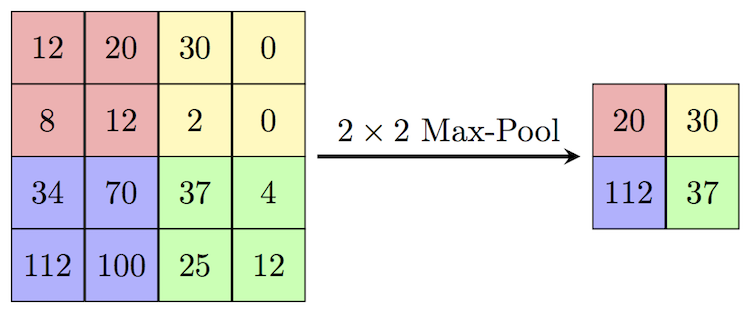
\includegraphics[scale=1.4]{Figures/maxpool_example.png}
    \caption{Exemple d'application de max-pooling 2x2 sur une entrée 4x4 \cite{noauthor_maxpoolsample2png_nodate}.}
    \label{fig:maxpool_example}
\end{figure}

L'average-pooling est une autre fonction de pooling qui s'exécute de la même façon que le max-pooling. Or, cette fois-ci il s'agit de la moyenne des éléments présents dans la fenêtre qui sont calculés.

La taille de la sortie résultant d'une opération de pooling peut être calculée. Supposons une entrée de taille $N \times C \times H \times W$, et un filtre de taille $(h, w)$. L'opération de pooling est appliquée séparément sur chaque canal, et produit la sortie de taille $N \times C \times [H/h] \times [W/w]$.

Par défaut, le pooling utilise un padding de zéro et un stride égal à la taille du filtre. 

\subsection{Normalisation par lots}
\label{subsec:batch_norm}

La normalisation par lots (batch normalization) est un procédé visant à accélérer et stabiliser l'entraînement des réseaux de neurones, ce qui peut améliorer leurs performances. Succinctement, son objectif est de maintenir des statistiques d'activations correctes, afin d'éviter qu'une couche doive s'adapter aux changements d'activations de la couche précédente en plus de ses propres changements. 

Pendant l'entraînement, la normalisation par lots ajuste et redimensionne les valeurs d'entrée en fonction de la moyenne et de la variance calculée dans le lot en cours. Lors des tests, elle utilise les moments empiriques estimés pendant la phase d'entraînement.

\subsection{Sauts de connexions}
\label{subsec:skip_connections}

Les sauts de connexion sont un type de raccourci qui relient la sortie d'une couche à une entrée qui n'est pas à la suite de cette dite couche. Ceux-ci sont notamment utilisés dans les réseaux neuronaux résiduels, mais également dans d'autres types d'architecture. Le principe est très simple, il s'agit d'une connexion qui crée un nouveau chemin qui saute un nombre défini de couches, puis qui va à s'insérer à l'entrée d'une autre couche soit par concaténation, addition, multiplication, etc..

La figure \ref{fig:skip_connections} illustre très bien ce principe. L'entrée du bloc A est à la fois passée dans le bloc A, et additionnée avec la sortie de ce même bloc et plus loin même additionné avec l'entrée et la sortie du bloc C.

\begin{figure}[hbt!]
    \centering
    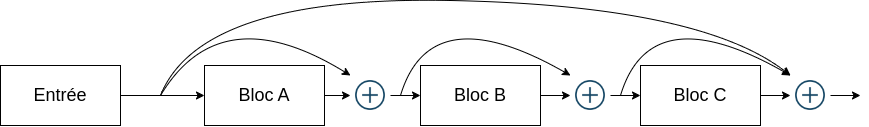
\includegraphics[scale=0.45]{Figures/skip_connections.png}
    \caption{Exemple de sauts de connexions.}
    \label{fig:skip_connections}
\end{figure}

L'utilisation des sauts de connexions permet de diminuer l'effet de la disparition du gradient. Ce fléau se produit lorsque le gradient est très petit. Comme la mise à jour des poids utilise une valeur proportionnelle à la dérivée de l'erreur par rapport au poids en question, celui-ci tend à disparaître pouvant provoquer l'arrêt de l'apprentissage.

\newpage

\section{YOLOv8}
\label{sec:yolov8}

Le premier modèle utilisé dans ce travail est un réseau de neurones convolutifs très populaire issu de la famille \acrfull{yolo} nommé YOLOv8. Sa première version publiée en juin 2015 \cite{redmon_you_2016} s'est fait connaître pour sa grande vitesse et ses hautes performances dans la détection et segmentation d'images. Présentés dans son article, \acrshort{yolo} et sa variante Fast YOLO obtiennent respectivement un \acrshort{map} de 63.4 pour 45 images par seconde, et un \acrshort{map} de 52.7 pour 155 images par secondes [table 1], un ratio de performances beaucoup plus élevé que les modèles couramment utilisés à ce moment-là. Cela en a fait un excellent choix pour des applications en temps réel.

Amélioré au fil des années, YOLOv8 est la dernière version développée par Utralytics utilisant les dernières avancées en deep learning et vision par ordinateur, qui propose des performances inégalées en termes de vitesse et de précision \cite{ultralytics_home_nodate}.

\subsection{Description du modèle}

Afin de comprendre comment fonctionne le modèle, reprenons l'implémentation initiale de YOLO mise au point par Joseph Redmon, et Santosh Divvala. Contrairement aux modèles proposés jusqu'alors, qui parcouraient plusieurs fois l'image traitée, \acrshort{yolo} propose une approche différente qui parcourt l'image une seule fois. Le principe est simple, comme illustré sur la figure \ref{fig:the_yolo_detection_system}, l'image en entrée est passée à un réseau neuronal convolutif qui va prédire simultanément de multiples boîtes de délimitations, et leurs probabilités d'appartenance à une classe.

\begin{figure}[hbt!]
    \centering
    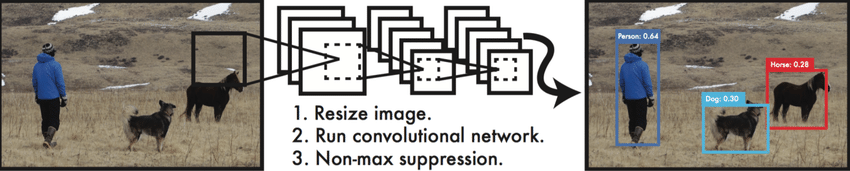
\includegraphics[scale=0.45]{Figures/The-YOLO-Detection-System-17.png}
    \caption{Système de détection de YOLO \cite{noauthor_figure_nodate-1}.}
    \label{fig:the_yolo_detection_system}
\end{figure}

Dans le but de réaliser des prédictions, le réseau de neurones utilise les caractéristiques de toute l'image pour déterminer chaque boîte de délimitation. Le système divise l'entrée en une grille de taille $S \times S$. Si le centre d'un objet se trouve dans une cellule de la grille créée, cette dernière va s'occuper de détecter l'objet. Chaque cellule prédit $B$ boîtes de détection contenant chacunes les éléments suivants : les coordonnées ($x, y$), la longueur, hauteur de l'objet ($w, h$), et le score de confiance. Ce dernier reflète à quel point le modèle est confiant qu'une boîte contienne un objet et l'exactitude de cette prédiction. La confiance est définie formellement par :

\[Confidence = Pr(Object) \cdot IOU^{truth}_{pred}\]

Où nous voyons qu'il s'agit de la probabilité de l'existence d'un objet multiplié par l'intersection sur l'union (voir chapitre \ref{sec:iou}) entre la prédiction et la réalité. Par ailleurs, chaque cellule prédit également la probabilité de chaque classe. Lors de la phase de test, cette valeur est multipliée avec les scores de confiance prédits, ce qui nous retourne le score de confiance de chaque classe donnée pour chaque boîte. Ce score prend en compte la probabilité d'occurrence de la classe donnée dans la boîte et également à quel point la boîte prédit l'objet. La figure \ref{fig:yolo_system_detection_class_and_boxes} illustre ce principe.

\begin{figure}[hbt!]
    \centering
    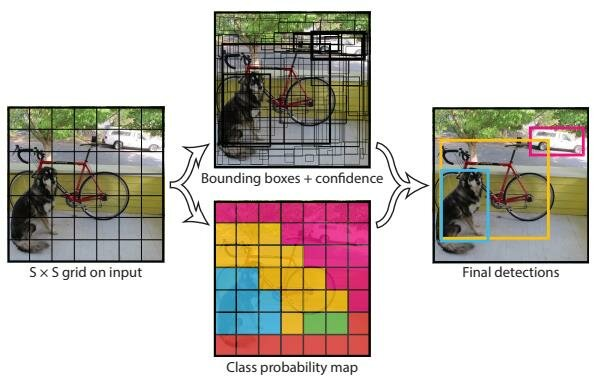
\includegraphics[scale=1.4]{Figures/yolo_system_detection_class_and_boxes.png}
    \caption{Le modèle de YOLO \cite{noauthor_figure_nodate-2}.}
    \label{fig:yolo_system_detection_class_and_boxes}
\end{figure}

Regardons à présent d'un peu plus près l'architecture du réseau représentée sur la figure \ref{fig:yolo_architecture}. Celle-ci contient 24 couches de convolutions suivies par 2 couches complètement connectées qui vont générer une sortie de taille $S \times S \times (B \cdot 5 + C)$ où $S$ correspond à la taille de la grille, $B$ le nombre de boîtes par cellules, et $C$ le nombre de classes.

\begin{figure}[hbt!]
    \centering
    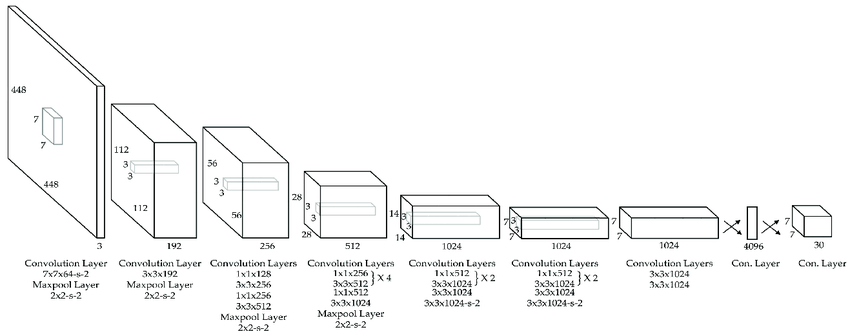
\includegraphics[scale=0.5]{Figures/yolo_architecture.png}
    \caption{Architecture de YOLO \cite{noauthor_figure_nodate-3}.}
    \label{fig:yolo_architecture}
\end{figure}

À présent que le modèle de base a été défini, nous pouvons résumer brièvement l'évolution de celui-ci. En 2016 sort YOLOv2 aussi connut sous le nom de YOLO9000 \cite{redmon_yolo9000_2016}, améliorant YOLO. Cette version conçue pour être plus rapide et précise est aussi capable de détecter une plus grande variété de classes. Ceci est possible grâce à l'utilisation d'un réseau de base appelé Darknet-19 exploitant les avantages de la batch normalization (\ref{subsec:batch_norm}), mais aussi grâce aux boîtes d'ancrage. Celles-ci sont un ensemble de boîtes de délimitations de différents formats et tailles prédéfinies, qui permettent de détecter une plus grande variété d'objets.\\

En 2018 YOLOv3 est publié \cite{redmon_yolov3_2018}. Celui-ci utilise une version améliorée du réseau de base appelé Darknet-53. YOLOv3 améliore également l'utilisation des boîtes d'ancrages en leur permettant de modifier leur échelle et leur octroyant une plus grande variété de formats pour correspondre au mieux aux objets détectés. Finalement, ce modèle introduit le concept de \acrfull{spp}, qui expliqué simplement permet de se débarrasser de la contrainte d'utiliser une image de taille fixe.\\

YOLOv4 introduit en 2020 \cite{bochkovskiy_yolov4_2020} utilise une nouvelle architecture nommée CSPDarknet53, une variante de l'architecture ResNet conçue pour la détection d'objet. Il est le premier à décomposer le modèle en plusieurs parties (modèle de base, cou, et tête). Il garde la même tête de détection utilisée par YOLOv3, mais modifie la génération des boîtes d'ancrages.\\

Apparu également en 2020 YOLOv5 \cite{jocher_yolov5_2020} possède un nouveau réseau de base plus complexe appelé EfficientDet. Il réutilise les principes des précédents modèles tout en les améliorant. Cela lui permet d'obtenir de meilleures performances et une meilleure généralisation à un plus grand ensemble de classes.\\

En 2022 deux versions de YOLO sortent à quelques mois d'intervalle, la v6 \cite{li_yolov6_2022} et la v7 \cite{wang_yolov7_2022}. Les deux proposent leurs propres améliorations vis-à-vis de leurs prédécesseurs que nous n'aborderons pas dans ce travail. YOLOv6 a été pensé pour être utilisé dans l'industrie, et YOLOv7 à sa sortie a surpassé tous les détecteurs d'objets en termes de vitesse et de précision.\\

Finalement en janvier 2023, la dernière version de YOLO développé par Utralytics sort. Lors de l'écriture de ce rapport, YOLOv8 n'a pas encore d'article dédié \cite{jocher_ultralytics_2023}. 

YOLOv8 propose cinq versions de tailles différentes, permettant de facilement choisir une version du modèle en fonction de ses besoins. La différence réside dans le nombre de filtres utilisés par les convolutions, et la profondeur du module C2f. Le modèle est capable de réaliser différentes tâches de vision par ordinateur telles que : la détection d'objet, la segmentation, l'estimation de pose, le suivi, et la classification. Son architecture décrite par la figure \ref{fig:yolov8_architecture} est composée de plusieurs éléments clefs. Il contient un réseau de base similaire à celui de YOLOv5, une couche de \acrfull{sppf}, un module C2f, et un module de détection. Le réseau de base s'occupe d'extraire les caractéristiques principales de l'entrée, puis cette sortie est passée à la couche \acrshort{sppf} qui à l'aide des couches de convolutions la suivant, vont traiter les caractéristiques à différentes échelles. Le module C2f est l'amélioration d'un module déjà existant en YOLOv5 et permet de se passer de la partie "cou" de l'architecture. Il s'agit d'une version accélérée du Cross Stage Partial Bottleneck utilisant deux convolutions, qui a pour but de concaténer les caractéristiques principales à de l'information contextuelle afin d'améliorer la précision de la détection. Finalement, le module de détection utilise un modèle sans ancrage avec une tête découplée afin d'exécuter indépendamment les tâches de classification, régression, ou encore de détection d'objet. Concernant le modèle sans ancrages, celui-ci utilise également un système de grille comme pour les boîtes à ancrages. La différence réside dans le fait que lorsqu'un objet est détecté dans une cellule, la première va estimer l'écart du centre de l'objet à partir du centre de la cellule, mais aussi sa hauteur et largeur. La deuxième va quant a elle estimer l'écart de l'objet détecté par rapport à des ancres prédéfinies.

\begin{figure}[hbt!]
    \centering
    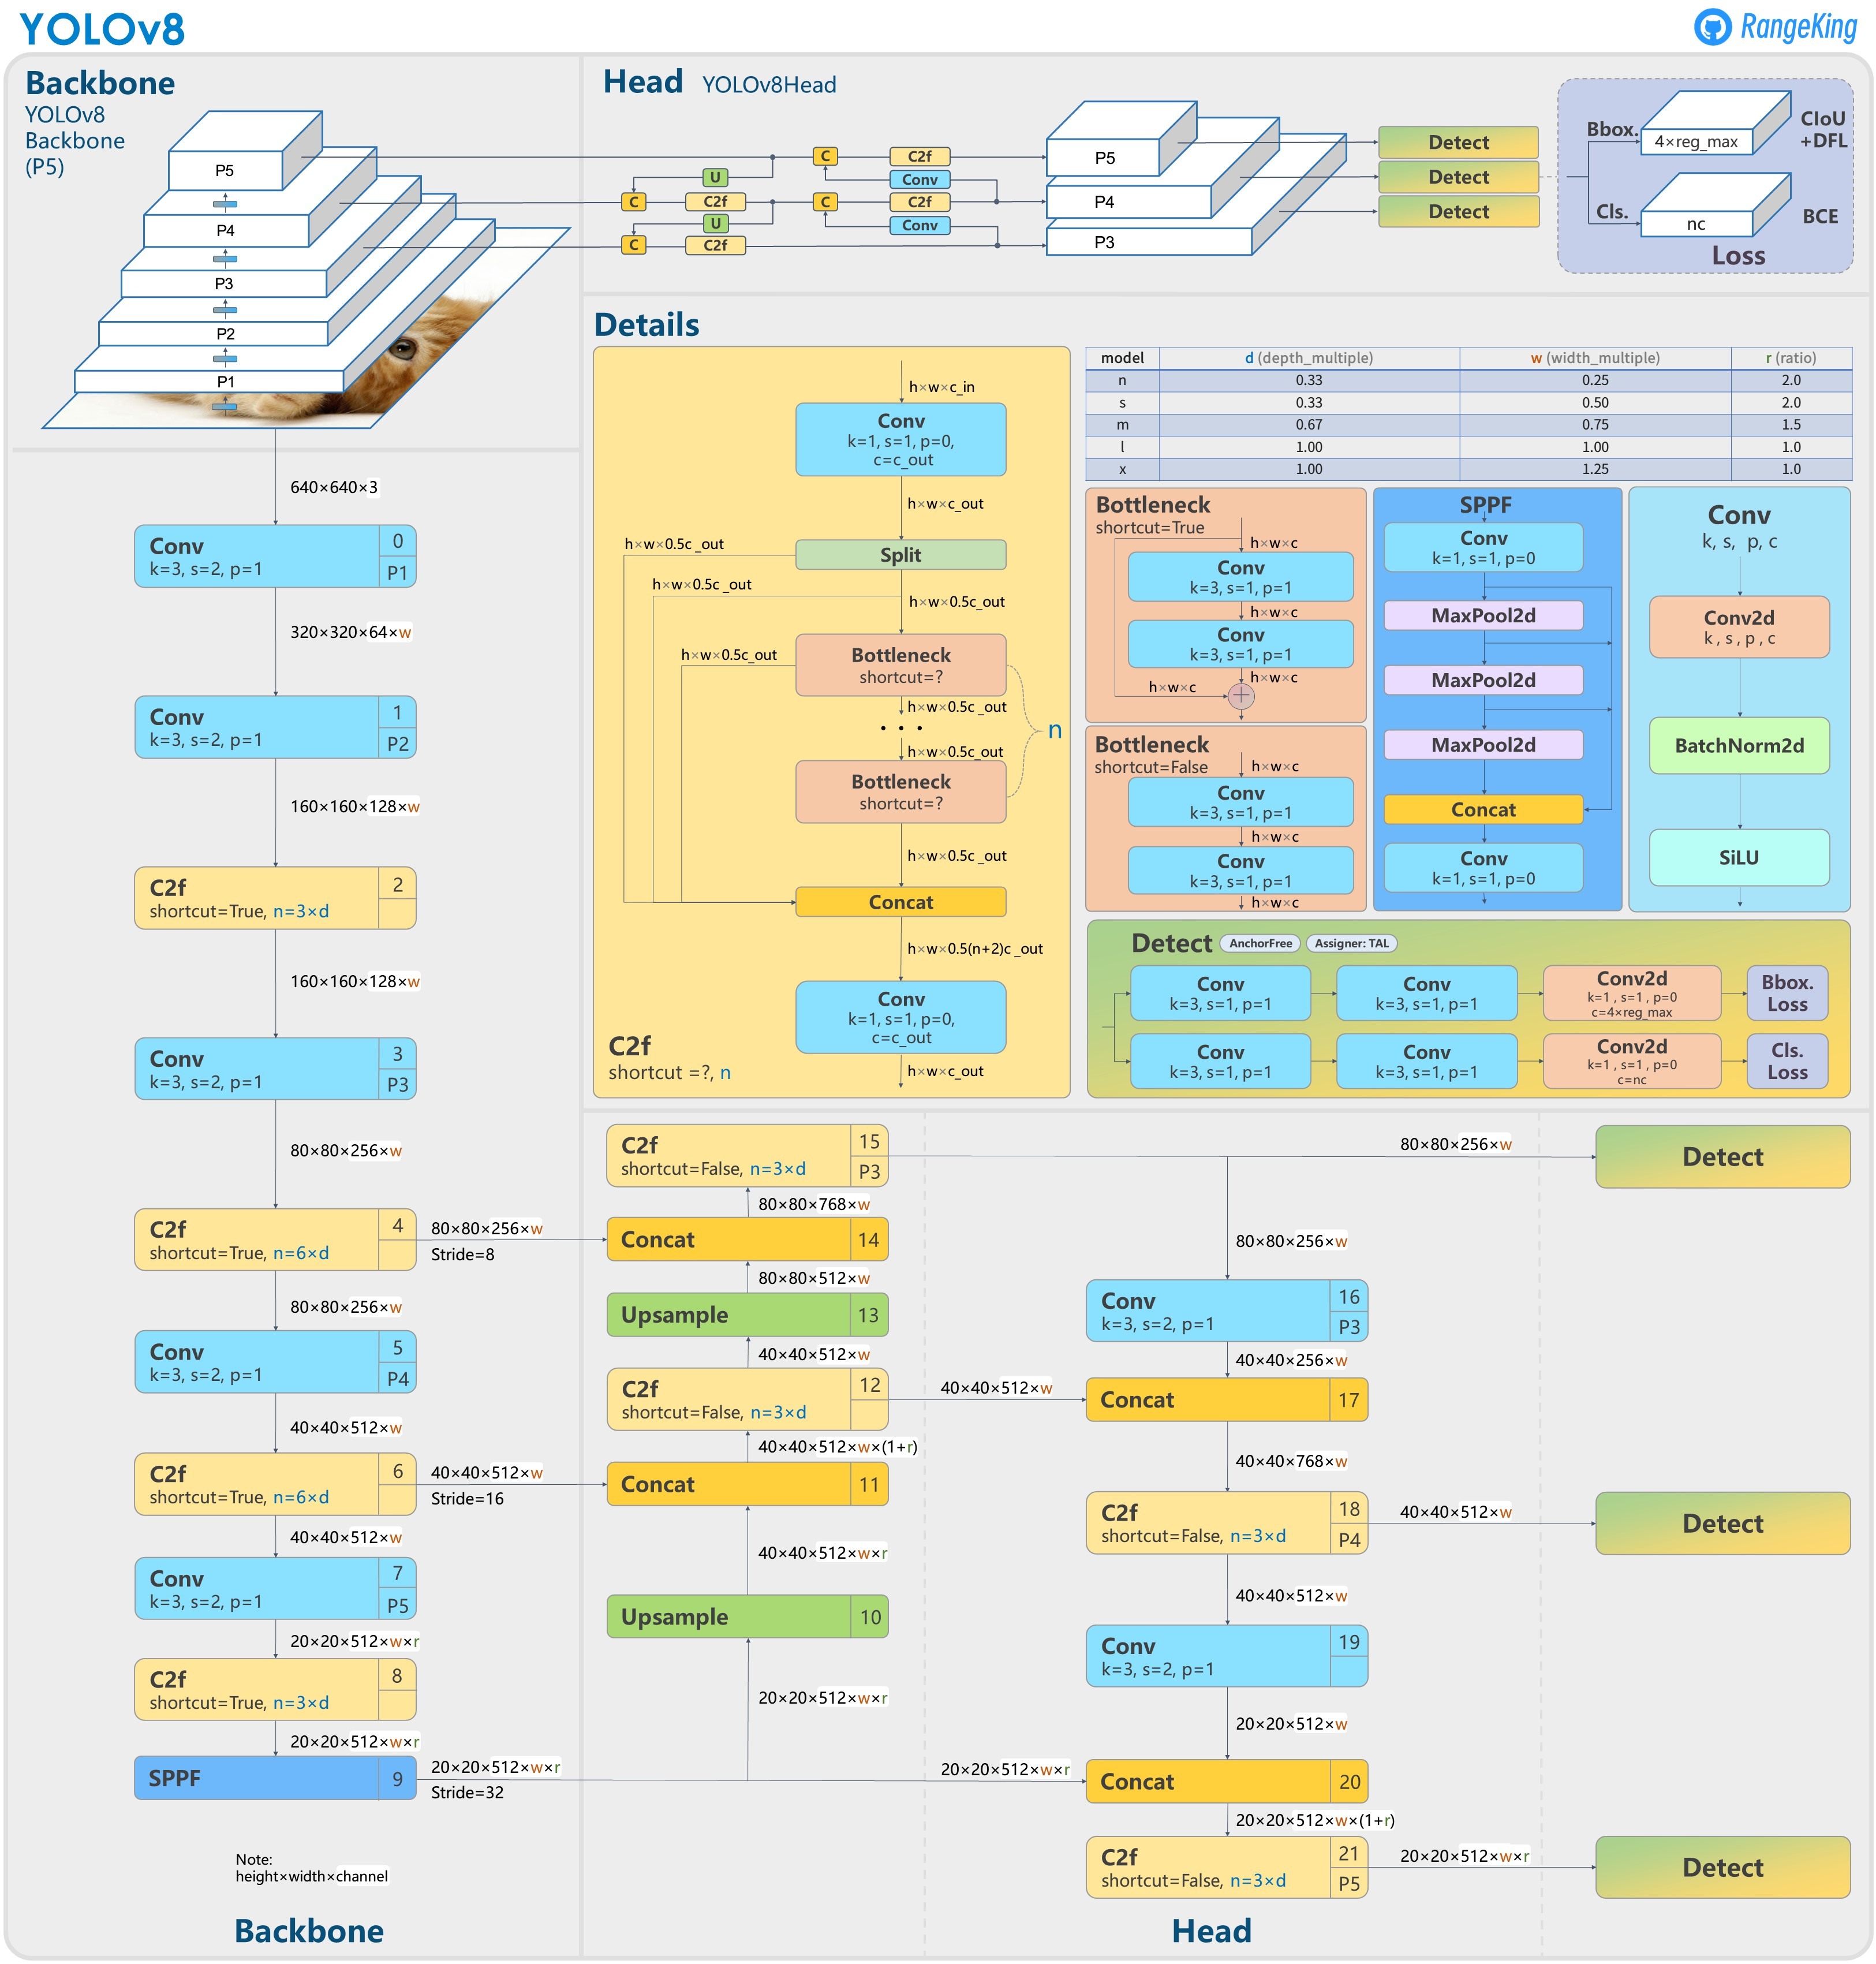
\includegraphics[scale=0.17]{Figures/yolov8_architecture.jpg}
    \caption{Architecture de YOLOv8 \cite{noauthor_brief_nodate}.}
    \label{fig:yolov8_architecture}
\end{figure}

\subsection{Utilisation du modèle}
\label{subsec:yolov8_utilization}

La version de YOLOv8 proposée par Ultralytics a été développée à l'aide de la bibliothèque Pytorch sur Python. Étant donné que nous souhaitons synthétiser le modèle à l'aide du paquet Python \acrshort{hls4ml} (\ref{HLS4ML}), et que celui-ci ne supporte que partiellement la bibliothèque Pytorch, nous avons réfléchi à deux approches différentes impliquant la bibliothèque Keras qui est supportée, tout en nous laissant l'accès au code pour pouvoir quantifier le code à l'aide de la librairie QKeras.

La première consistait à développer le modèle à partir de zéro. Malgré l'architecture et le code Pytorch à disposition, réaliser une telle implémentation restait un travail trop conséquent. Cependant, même si cette solution n'a pas été retenue, nous avons tout de même pu contribuer à la correction de l'architecture publiée.\\

La deuxième approche, qui est celle retenue, consiste à reprendre la librairie KerasCV \cite{noauthor_kerascv_2023} contenant leur propre implémentation en Keras du modèle YOLOv8. Cette solution nous permet de nous concentrer sur l'utilisation pure du modèle tout en nous donnant l'accès complet à leur code pour le modifier comme souhaité.\\

Afin de travailler librement sur le code de KerasCV nous avons forké et modifié leur code tout en développant nos propres scripts. Pour commencer, nous avons réalisé une légère modification dans le code source. Celle-ci concerne la constante \verb|BOX_REGRESSION_CHANNELS| qui est initialisée à 64. Même si elle ne possède pas le même nom que sur l'architecture de YOLOv8, cette dernière est utilisée comme la variable \verb|reg_max| qui correspond à la plage maximale des paramètres des boîtes d'ancrages \cite{noauthor_what_nodate}. Nos images en entrée étant déjà petites, $49 \times 64$, le rayon des jets présents dans celles-ci l'est encore plus et est égales à $4$ pixels. Finalement, nous trouvons empiriquement que la valeur 16 est celle qui donne les meilleurs résultats.\\

Avec notre modèle fonctionnel, nous avons pu réaliser plusieurs entraînements, et tester les prédictions de celui-ci. Lorsque YOLOv8 effectue une prédiction, celui-ci va nous retourner trois listes. La première nommée "boxes" possède les informations relatives à la boîte concernant la prédiction. Elle contient les coordonnées $(x, y)$ mais également la hauteur et largeur de l'objet. La deuxième nommée "classes", contient la classe à laquelle appartient chaque détection. Puis la troisième nommée "confidence", est constituée du score de confiance du modèle au sujet de la prédiction concernée.\\

Concernant les images à fournir au modèle, comme expliqué par Glenn Jocher \cite{noauthor_image_nodate}, créateur de YOLOv5 et YOLOv8, celui-ci travaille sur des entrées dont la taille est un multiple $32$. Cependant, si cela n'est pas le cas, l'image sera automatiquement redimensionnée pour répondre à cette exigence. Pour éviter toute modification de nos images, nous avons décidé d'augmenter la taille de notre matrice vers le premier multiple de $32$, et obtenons ainsi une nouvelle matrice de $64 \times 64$. L'axe $\phi$ n'est pas modifié étant donné qu'il est déjà égal à cette taille. En revanche, l'axe $\eta$ est augmenté par des indices dont la valeur est définie à $0$.\\

Un point que nous avons constaté en travaillant sur notre modèle est que le nombre de paramètres indiqué sur l'implémentation originale en Pytorch n'est pas identique à celle de Keras. Ainsi, Ultralytics présente le nombre de paramètres suivants en fonction de la taille du modèle comme indiqué sur la table \ref{tab:nb_params_yolov8_pytorch}.

\begin{table}[!ht]
    \caption{Nombre de paramètres pour chaque modèle de YOLOv8 Pytorch}
    \label{tab:nb_params_yolov8_pytorch}
    \rowcolors{2}{gray!25}{white}
    \centering
    \begin{tabular}{ |c||c|  }
        \hline
        \rowcolor{gray!50}
        Modèle & params (M)\\
        \hline
        YOLOv8n & 3.2\\
        YOLOv8s & 11.2\\
        YOLOv8m & 25.9\\
        YOLOv8l & 43.7\\
        YOLOv8xl & 68.2\\
        \hline
    \end{tabular}
\end{table}

Alors que les valeurs des modèles issus de l'implémentation KerasCV correspondent à celles décrites par la table \ref{tab:nb_params_yolov8_kerascv}.

\begin{table}[!ht]
    \caption{Nombre de paramètres pour chaque modèle de YOLOv8 KerasCV}
    \label{tab:nb_params_yolov8_kerascv}
    \rowcolors{2}{gray!25}{white}
    \centering
    \begin{tabular}{ |c||c|  }
        \hline
        \rowcolor{gray!50}
        Modèle & params (M)\\
        \hline
        YOLOv8xs reduced 16x & 0.025779\\
        YOLOv8xs reduced 8x & 0.0679\\
        YOLOv8xs reduced 4x & 0.225522\\
        YOLOv8xs reduced 2x & 0.834286\\
        YOLOv8xs & 3.225894\\
        YOLOv8s & 12.856342\\
        YOLOv8m & 25.665798\\
        YOLOv8l & 39.401462\\
        YOLOv8xl & 61.535974\\
        \hline
    \end{tabular}
\end{table}

Cette différence peut s'expliquer simplement par le fait qu'il s'agit de deux librairies distinctes dont l'implémentation de chaque couche n'est pas identique. Par ailleurs, les noms des modèles sont légèrement différents, mais ils correspondent à la même logique.\\

Finalement, nous avons tenté de synthétiser la version de YOLOv8 à l'aide de \acrshort{hls4ml}. Nous nous sommes retrouvés bloqués par des limitations d'implémentations du paquet. En effet, KerasCV a imbriqué le modèle de base (backbone) dans le modèle YOLOv8. Or, la version 0.7.1 de \acrshort{hls4ml} n'arrive malheureusement pas à extraire les couches d'un modèle imbriqué. Malgré plusieurs essais pour dérouler cette dernière et prémâcher le travail à \acrshort{hls4ml}, celui-ci n'arrivait pas à comprendre ces couches. Une piste suggérée par Pablo Strasser un collaborateur scientifique à la HEG, était d'exporter le modèle Keras en ONNX, un format ouvert pour représenter les modèles de machine learning. Cependant, \acrshort{hls4ml} ne supportait pas certaines couches de ce format utilisées par YOLOv8. De plus, certaines couches personnalisées définies dans le code de KerasCV ne sont pas prises en charge par \acrshort{hls4ml}, nécessitant le développement de l'implémentation HLS de ces dernières.

Ainsi, comme le modèle ne pouvait pas être synthétisé sans une réécriture profonde du code et pour une question de temps, nous avons décidé de ne pas quantifier le modèle, mais de tout de même tester ses performances sur notre problème. À la fin de notre travail sur ce modèle, nous avons des scripts permettant d'entraîner le modèle, de l'évaluer, de générer des labels ou des images, mais également de visualiser les résultats obtenus sous forme de tableaux ou de graphes à l'aide de diverses métriques.

\subsection{Génération des labels}
\label{subsec:yolov8_labels_generation}

Afin de pouvoir entraîner le modèle à détecter des jets, il a fallu générer les labels des images passées en entrée. Tout comme pour la génération des images, nous avons voulu stocker les labels dans des fichiers .npy pour les avantages qu'ils présentent. Ce format impose cependant une contrainte, il faut que les tableaux stockés soient tous de même taille. Étant donné que le nombre de jets par image n'est pas fixe, nous avons décidé d'ajouter une classe qui nous permet d'étoffer notre tableau si besoin afin d'obtenir des tableaux d'une taille fixe. Cette "nouvelle classe" est notée la classe 0 et possède toujours les mêmes coordonnées, c'est-à-dire en $(x, y)$  $(55, 32)$. Celle-ci correspond à la partie paddée de l'image qui ne contient aucune information. Dans le cas où il s'agit bien d'un jet que nous souhaitons labéliser, il sera noté comme appartenant à la classe 1 et aux coordonnées $\eta \times \phi$ de la matrice où il se trouve.

Un label est donc défini de la manière suivante : $coordonn\acute{e}e \: \eta, \: coordonn\acute{e}e \: \phi, \: H, \: W, \: classe$.\\

Concernant le nombre de labels, nous avons repris la logique des fichiers .h5. Ceux-ci sont également contraints d'indiquer une taille fixe qui a été définie à 30. C'est cette même constante que nous avons réutilisé.

Lors de la génération des labels, nous vérifions que le jet en cours de labélisation soit compris dans un intervalle plus restreint que celui posé de base. En effet, nous souhaitons ne pas prendre en compte les bords de l'image qui sont plus sensibles dans le cadre de la détection, car ces derniers peuvent contenir un jet partiel pouvant être ou non reconnu comme tel. Comme nous connaissons le rayon d'un jet qui est de 0.4, nous allons travaillé dans l'intervalle $\eta \in \mathbb{R} : \eta \in [-2;2]$ et $\phi \in \mathbb{R} : \phi \in [-2.75;2.75]$ afin de ne pas être confrontés à ces cas.

En ce qui concerne la hauteur et la largeur des jets, nous réutilisons la valeur du rayon d'un jet sur les deux axes ce qui nous donne approximativement 4 pixels pour les deux axes. Étant donné que nous réalisons des conversions d'échelles sur des valeurs arrondies, nous voulons nous assurer d'englober la totalité d'un jet. C'est pourquoi nous décidons d'utiliser 5 pixels de rayon.

De par le format d'entrée attendu par le modèle, les labels doivent être décomposés en deux parties de la façon suivante : $coordonn\acute{e}e \: \eta, \: coordonn\acute{e}e \: \phi, \: H, \: W$ et $classe$. Nous allons donc créer deux tableaux contenant ces informations de façons séparées.

\subsection{Evaluation du modèle}
\label{subsec:yolov8_model_evaluation}

Lorsque le modèle a été entrainé, il est crucial de pouvoir l'évaluer. Pour ce faire, nous avons développé un script d'évaluation afin de générer les résultats nécessaires au calcul des différentes métriques utilisées. Pour cela, nous allons nous servir de nos images et labels dédiés pour l'évaluation.

Nous allons tout d'abord sélectionner pour chaque événement, les jets qui sont dans la zone de détection que nous avons précédemment définie. Suite à cette étape, nous allons parcourir les détections de notre modèle en ne prenant en compte que celles qui ont été réalisées pour la classe 1 (correspondant aux jets), et dans l'intervalle $\eta \in \mathbb{R} : \eta \in [-2;2]$ et $\phi \in \mathbb{R} : \phi \in [-2.75;2.75]$.

Finalement, nous utilisons le seuil de confiance assigné à chaque détection pour déterminer lesquelles doivent être prises en considération et qui seront acceptées ou rejetées par la suite à l'aide de l'intersection sur union (\ref{sec:iou}). 

Pour identifier si un jet détecté est correct ou non, nous allons parcourir tous les labels de l'image en testant à chaque fois si leur \acrshort{iou} est supérieur à un seuil fixé en avance.

\newpage

\section{ResNet18 + Tête}
\label{sec:resnet18}

Le deuxième modèle utilisé est un réseau neuronal convolutif personnalisé. Celui-ci utilise comme base ResNet18 auquel une tête a été ajoutée afin de modifier le classifieur en un détecteur. Ainsi, nous pouvons obtenir des coordonnées et un score de confiance en sortie. Ce modèle a été mis en point avec la volonté de proposer une implémentation simple, possédant peu de paramètres, des performances correctes, et qui puisse être synthétisée avec \acrshort{hls4ml}. ResNet18 répondant à ces critères, nous l'avons donc sélectionné.

\subsection{Description du modèle}

Commençons tout d'abord par décrire le modèle de base. ResNet18 est un réseau neuronal résiduel présenté en 2015 par Kaiming He, Xiangyu Zhang, Shaoqing Ren, et Jian Sun \cite{he_deep_2015} qui propose une architecture facilitant l'entraînement de réseaux profonds. Ce type de réseau utilise les sauts de connexion (\ref{subsec:skip_connections}) afin de pouvoir construire des modèles profonds pouvant posséder un plus grand nombre de couches, tout en diminuant le problème de la disparition du gradient.

Dans l'article, les auteurs présentent cinq variantes de 18, 34, 50, 101, et 152 couches. Bien que les modèles plus profonds aient de meilleurs résultats, nous choisissons le réseau de 18 couches, car celui-ci est le plus petit et donc le plus rapide, tout en proposant des performances acceptables. L'architecture de ResNet18 est illustrée à la figure \ref{fig:resnet18_architecture}.

Le modèle prend en entrée dans sa version originale une image de 224x224x3 où 224x224 correspond à la taille de l'image, et le 3 représente les canaux rouge, vert, bleu. L'entrée est passée dans une première couche de convolution possédant un noyau de $(7,7)$, un stride de $(2,2)$, et un padding de $(3,3)$. Une opération de max-pooling, avec une fenêtre de $(3,3)$ et un stride de $(2,2)$, est par la suite appliquée afin de réduire la dimensionnalité de l'image.

La partie principale du réseau est constituée de huit blocs résiduels. Chacun d'entre eux contient deux couches de convolutions d'un noyau de $(3,3)$ ainsi qu'un saut de connexion (représenté par les flèches pleines sur la figure \ref{fig:resnet18_architecture}) entre l'entrée et la sortie du bloc qui est additionné à ce dernier. Le nombre de filtres double tous les 4 blocs dans l'ordre suivant : $64, 128, 256, 512$. Entre deux blocs d'un nombre de filtres différents, le saut de connexion (représenté par les flèches traitillés sur la figure \ref{fig:resnet18_architecture}) est légèrement modifié et passe par une convolution d'un noyau de $(1,1)$, et un stride de $(2,2)$ afin que la sortie soit de même dimension.

La sortie des ces blocs résiduels est passé dans une opération de global average pooling qui va calculer la moyenne de chaque dimension et ainsi obtenir une sortie de taille $(512,)$.

A ce stade le modèle ResNet18 va passer le résultat de la couche précédente dans une couche de neurones pleinement connectés afin de réaliser la classification sur les mille classes présentes sur ImageNet (une base de données d'images labélisées). C'est à cette étape que nous allons retirer cette couche afin d'y ajouter notre tête de détection, représentée à la figure \ref{fig:resnet18+head_architecture}. Celle-ci est composée d'un nombre $n$ de blocs de détection (D.B. pour Detection Block) correspondant à la manière dont l'image a été subdivisée lors de la labélisation (\ref{subsec:resnet18+head_label_generation}). Chaque bloc va ainsi contribuer à la détection d'un objet dans une région spécifique de l'image. La couche Dense avec deux neurones en sortie va prédire les coordonnées $(x,y)$ de l'emplacement d'un jet, et la couche Dense avec un seul neurone en sortie va établir un score de confiance. Ces deux sorties sont concaténées entre elles, avant d'être à leur tour concaténées avec le reste des prédictions.

\begin{figure}[hbt!]
    \centering
    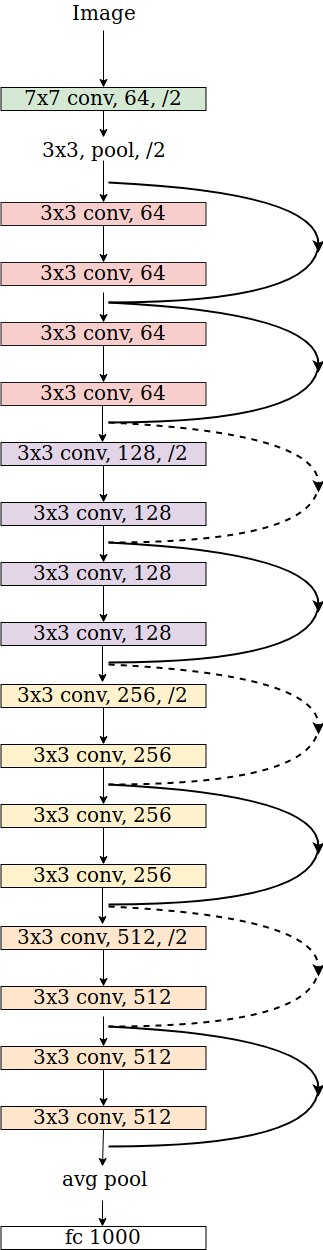
\includegraphics[scale=0.4]{Figures/resnet18_architecture.png}
    \caption{Architecture de ResNet18 \cite{thatsnotmyname71_what_2019}.}
    \label{fig:resnet18_architecture}
\end{figure}

\newpage

\begin{figure}[hbt!]
    \centering
    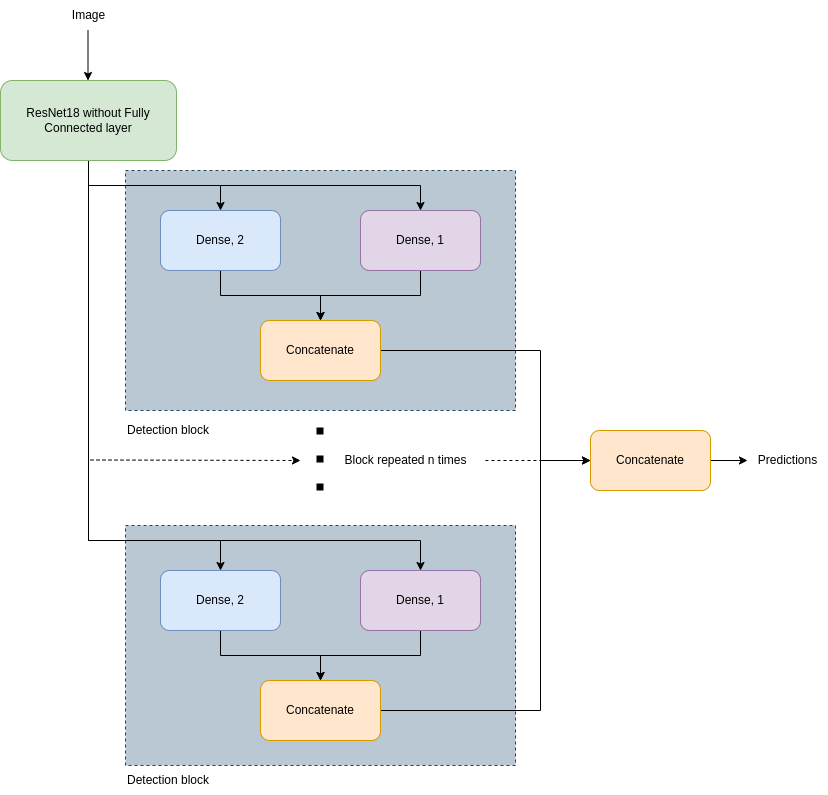
\includegraphics[scale=0.5]{Figures/resnet18+head_architecture.png}
    \caption{Architecture de ResNet18 avec sa tête de détection.}
    \label{fig:resnet18+head_architecture}
\end{figure}

\subsection{Développement de la tête}

Avant d'obtenir la tête utilisée actuellement par notre modèle, nous avons fait plusieurs itérations en les testant à chaque fois. L'idée initiale était d'utiliser un \acrshort{mlp} qui retournerait une sortie similaire à celle de \acrshort{yolo}, c'est-à-dire les coordonnées $(x, y)$, la hauteur et largeur de l'objet, ainsi qu'un score de confidence. Comme nous ne travaillons qu'avec une seule classe, nous avons déjà retiré cette sortie. Nous nous sommes rapidement rendu compte que le modèle peinait à travailler avec la hauteur et largeur des jets. Comme ceux-ci ont toujours le même rayon, nous avons décidé de retirer ces valeurs afin de faciliter l'apprentissage du modèle. Suite à cette étape, nous avons constaté qu'un \acrshort{mlp} plus petit menait à de meilleures performances, jusqu'à ne garder qu'une couche de neurones.

Le neurone générant les coordonnées $(x, y)$ possède un \acrshort{relu} comme fonction d'activation étant donné que nous souhaitons obtenir les coordonnées sur notre matrice. Le neurone générant le score de confiance utilise quant à lui une sigmoïde afin d'obtenir une valeur entre 0 et 1.

\subsection{Utilisation du modèle}

Lors de l'implémentation de notre modèle, nous avons repris la structure de ResNet18 à laquelle nous avons ajouté des blocs de détection en remplacement de la couche de neurones entièrement connectés. De plus, nous avons intégré des couches de normalisation par lots après chaque convolution pour tirer parti de ses avantages.

L'objectif restant le même que pour YOLOv8, nous avons réutilisé les scripts développés précédemment. Nous avons notamment gardé les mêmes images que pour YOLOv8. En effet, la génération des labels étant différente et subdivisant nos images en sous-matrices de taille égales, il était plus pratique de continuer à travailler avec des matrices carrées.

Le modèle retourne en sortie un Tensor avec les prédictions réalisées par chaque bloc de détection sous forme $(x, y, conf)$, où les deux premières valeurs correspondent aux coordonnées et la troisième au score de confiance concernant la présence d'un jet aux indices indiqués.

Concernant la taille du modèle, celle-ci varie en fonction du nombre de blocs de détection et de la taille des filtres de convolution, comme présenté sur la table \ref{tab:nb_params_resnet18+head}. Il est intéressant de noter le nombre de paramètres n'est pas affecté par la quantification du modèle.

\begin{table}[!ht]
    \caption{Nombre de paramètres pour chaque modèle de ResNet18+Tête et différentes tailles de blocs de détections (D.B.)}
    \label{tab:nb_params_resnet18+head}
    \rowcolors{2}{gray!25}{white}
    \centering
    \begin{tabular}{ |c||c|  }
        \hline
        \rowcolor{gray!50}
        Modèle & params (M)\\
        \hline
        (Q)ResNet18+Head 64 D.B. reduced 16x & 0.052008\\
        (Q)ResNet18+Head 64 D.B. reduced 8x & 0.190992\\
        (Q)ResNet18+Head 64 D.B. reduced 4x & 0.730464\\
        (Q)ResNet18+Head 64 D.B. reduced 2x & 2.855424\\
        (Q)ResNet18+Head 64 D.B. & 11.289408\\
        (Q)ResNet18+Head 16 D.B. & 11.215536\\
        (Q)ResNet18+Head 36 D.B. & 11.246316\\
        (Q)ResNet18+Head 121 D.B. & 11.377131\\
        \hline
    \end{tabular}
\end{table}

\subsection{Génération des labels}
\label{subsec:resnet18+head_label_generation}

Tout comme pour la génération des labels avec YOLOv8, nous allons réutiliser le format .npy et la contrainte liée, c'est-à-dire le besoin d'avoir des labels d'une taille fixe entre toutes les images. Par ailleurs, nous conservons la logique d'omettre les jets trop proches des bords de l'image, afin de travailler dans l'intervalle $\eta \in \mathbb{R} : \eta \in [-2;2]$ et $\phi \in \mathbb{R} : \phi \in [-2.75;2.75]$.\\

Contrairement à YOLOv8, l'ordre des labels impacte directement les performances du modèle. La méthode d'annotation choisie est donc cruciale pour obtenir de bons résultats.

Une approche naïve pourrait être d'ordonner la liste des jets d'une image par rapport à l'axe $\eta$ ou $\phi$ et de compléter la taille de cette dernière avec des éléments dans la zone paddée. Bien que cette implémentation soit simple et permette de choisir aisément un nombre arbitraire de neurones, lors de l'apprentissage les premiers neurones seront ceux qui verront un grand nombre de jets. Comme visible sur les figures \ref{fig:visulization_prediction_naive} et \ref{fig:visulization_prediction_naive_mean_std}, le premier neurone réalise des détections sur une grande surface de l'image, puis les neurones suivants réaliseront des détections sur une surface plus petite, jusqu'aux derniers neurones qui ne détecteront plus rien.\\

\begin{figure}[hbt!]
    \centering
    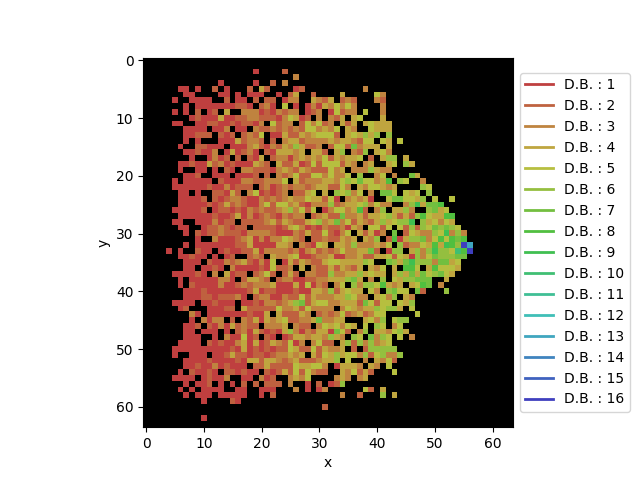
\includegraphics[scale=0.7]{Figures/visulization_prediction_naive.png}
    \caption{Visualisation de l'emplacement des prédictions de chaque bloc de détection du modèle entraîné par la méthode naïve pour le jeu de données "test" avec 16 blocs de détection (D.B.).}
    \label{fig:visulization_prediction_naive}
\end{figure}

\begin{figure}[hbt!]
    \centering
    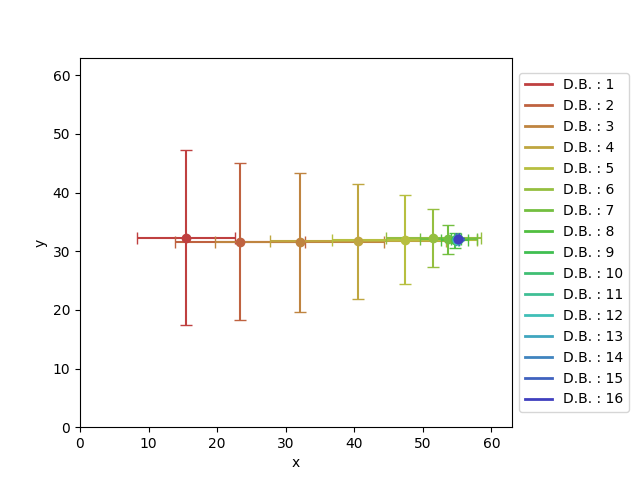
\includegraphics[scale=0.7]{Figures/visulization_prediction_naive_mean_std.png}
    \caption{Visualisation de la moyenne et de l'écart-type des prédictions de chaque bloc de détection du modèle entraîné par la méthode naïve pour le jeu de données "test" avec 16 blocs de détection (D.B.).}
    \label{fig:visulization_prediction_naive_mean_std}
\end{figure}

Une autre approche, qui est celle utilisée, consiste à découper l'image en un nombre de régions prédéterminé. Par exemple, si nous définissons ce nombre de zones à 16 pour notre image de taille $(64 \times 64)$, celle-ci va découper l'image en 16 sous-matrices d'une taille de $(16 \times 16)$. La figure \ref{fig:image_subdivided_like_labels_does} illustre cette application sur une image extraite des données avec en rouge la séparation entre les zones et en blanc le centre de chaque région.

\begin{figure}[hbt!]
    \centering
    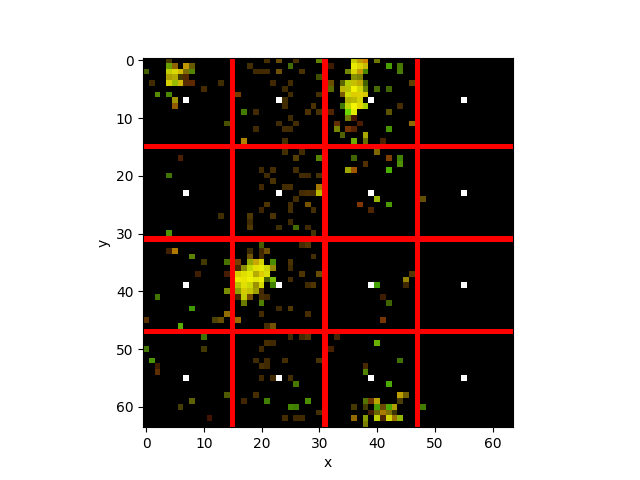
\includegraphics[scale=0.7]{Figures/image_subdivided_like_labels_does.png}
    \caption{Exemple d'image subdivisée en sous partie.}
    \label{fig:image_subdivided_like_labels_does}
\end{figure}

Dans un premier temps, chaque région va s'attribuer le jet le plus proche si celui-ci est dans un rayon donné. Celui-ci est déterminé par la taille des sous-matrices moins un, le tout divisé par deux. Par exemple dans le cas où l'image est décomposée en 16 parties, le rayon sera de $(16-1)/2=7.5$.

Dans un second temps, les éléments n'ayant pas été attribués lors de la première phase se répartiront parmi les régions sans jet en sélectionnant celles dont ils sont le plus proche.

Ce procédé comporte quelques limitations, en effet, chaque sous-matrice accueille un unique jet. Dans le cas où le nombre de régions n'est pas suffisant pour tous les répartir, certains seront alors manqués. C'est pour cela qu'il est important de connaître le nombre de jets maximums dans les expériences, afin de décomposer la matrice en un nombre de régions suffisantes. De plus, la seconde phase ne vérifie pas si un autre jet restant est plus proche de la sous-matrice sélectionnée. Cependant, la complexité inhérente à la gestion de ces cas étant élevée, et le temps nous faisant défaut, nous avons décidé de ne pas les gérer.\\

Lorsqu'un jet est attribué à une région, nous générons un label indiquant les coordonnées du jet, et attribuons la "classe" 1 à ce label pour indiquer qu'il y a bien quelque chose à détecter dans cette zone. Dans le cas où une région n'a pas eu de jet attribué, le label contiendra les coordonnées du centre de la zone avec la "classe" 0 correspondant à "rien à détecter".

Suite à la répartition, l'ordre de lecture des labels créés pour générer la liste liée est toujours identique. L'idée derrière cette méthode est que chaque bloc de détection apprenne à identifier les jets dans leur région, mais également un peu plus loin si nécessaire. Nous pouvons observer cela sur la figure \ref{fig:visulization_prediction_4_n_neurons}, ainsi que la répartition des blocs de détections sur l'image et leur déviation standard sur la figure \ref{fig:visulization_prediction_4_n_neurons_mean_std}.

\begin{figure}[hbt!]
    \centering
    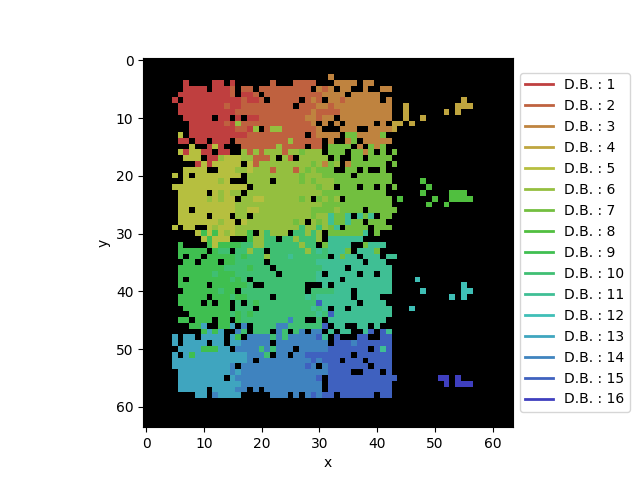
\includegraphics[scale=0.7]{Figures/visulization_prediction_4_n_neurons.png}
    \caption{Visualisation de l'emplacement des prédictions de chaque bloc de détection du modèle entraîné par la méthode de découpage de l'image pour le jeu de données "test" avec 16 blocs de détection (D.B.).}
    \label{fig:visulization_prediction_4_n_neurons}
\end{figure}

\begin{figure}[hbt!]
    \centering
    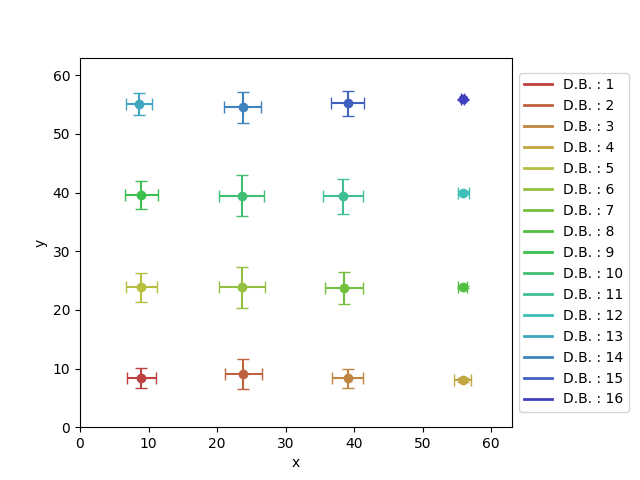
\includegraphics[scale=0.7]{Figures/visulization_prediction_4_n_neurons_mean_std.png}
    \caption{Visualisation de la moyenne et écart-type des prédictions de chaque bloc de détection du modèle entraîné par la méthode de découpage de l'image pour le jeu de données "test" avec 16 blocs de détection (D.B.).}
    \label{fig:visulization_prediction_4_n_neurons_mean_std}
\end{figure}

\break

\subsection{Évaluation du modèle}

L'évaluation de notre modèle est relativement similaire à celle réalisée pour YOLOv8 (\ref{subsec:yolov8_model_evaluation}). La principale différence réside dans la manière de calculer l'\acrshort{iou}. En effet, notre modèle ne nous retournant pas la largeur et la hauteur des boîtes de détection, nous définissons celle-ci manuellement aux mêmes valeurs que pour les labels de YOLOv8, c'est-à-dire à 5 pixels.

\subsection{Quantification du modèle avec QKeras}
\label{subsec:qkeras_quantization}

Dans l'optique de synthétiser notre modèle avec \acrshort{hls4ml}, nous avons utilisé la bibliothèque QKeras [\cite{noauthor_qkeras_2023}] afin de quantifier notre réseau de neurones. Cette approche consiste à réduire la précision des poids, activations, et gradients de notre réseau, afin de le rendre plus adapté à une implémentation sur \acrshort{fpga} où les ressources y sont limitées.

La quantification réalise une réduction du nombre de bits nécessaires pour représenter une valeur. Dans le cadre de ResNet18+Tête, cela aura pour effet de diminuer la précision des nombres, passant d'une représentation en virgule flottante à virgule fixe. Bien que cette diminution de précision puisse provoquer une baisse des performances, cette représentation étant similaire à celle des \acrshort{fpga}, les résultats obtenus devraient être similaires.

Lors de cette étape, nous avons uniquement modifié l'ensemble des couches de convolution, de Dense, de normalisation par lots, et d'activation par leurs versions quantifiées. Il est possible d'indiquer pour certaines de ces couches le nombre de bits à utiliser. Ainsi, nous avons décidé de travailler avec 16 bits, dont 6 sont utilisés pour représenter la partie entière.

Par ailleurs, la version quantifiée de la fonction d'activation sigmoïde propose soit une approximation assez pauvre, soit la possibilité d'utiliser la fonction définie par la librairie Keras. Étant donné que la qualité de cette fonction a un impact direct sur les performances de notre modèle, nous avons choisi d'utiliser la fonction définie par Keras.

\subsection{Synthétiser le modèle avec HLS4ML}
\label{subsec:r18_synthetize_with_hls4ml}

Afin de pouvoir implémenter notre modèle quantifié sur \acrshort{fpga}, nous devons d'abord le synthétiser à l'aide de \acrshort{hls4ml}. Lors de cette phase, nous nous sommes heurtés à plusieurs contraintes / limitations détaillées dans la section \ref{sec:hls4ml_limitations}.

En plus de ces dernières, les ressources nécessaires pour synthétiser un modèle avec \acrshort{hls4ml}, notamment la mémoire vive, dépendent de la taille de ce dernier. Même s'il est possible de modifier le "ReuseFactor" qui va indiquer combien de fois un élément peut être réutilisé, nous avons souhaité réaliser une synthèse de ResNet18+Tête avec un "ReuseFactor" de $1$, afin de minimiser la latence. C'est pourquoi nous travaillons pour cette partie sur une version de ResNet18 dont les filtres des convolutions ont été divisés par 16. Malgré cela, les dernières couches de convolution de notre modèle avec un kernel de $3 \times 3$ possèdent trop d'éléments, et ne peuvent malheureusement pas utiliser la stratégie "Latency", raison pour laquelle elles ont été définies à "Resource".

Il faut également prendre en compte que comme nous ne pouvions malheureusement pas réutiliser une variable dans notre modèle plus de trois fois, et étant donné que nous réutilisons la sortie de notre version raccourcie de ResNet18 deux fois dans chacun de nos blocs de détections, nous ne pouvons utiliser qu’un seul bloc pour la synthèse de notre modèle.

%----------------------------------------------------------------------------------------

% Results

\chapter{Résultats} % Main chapter title
\label{Results} % For referencing the chapter elsewhere, use \ref{Results} 

Dans ce chapitre nous allons aborder les résultats obtenus grâce à nos deux modèles et à leur différentes versions ou tailles de filtres. Chaque modèle a été entraîné cinq fois à partir de zéro, et ce pendant 500 (ou 1000 époques pour la version quantifiée) dans le but d'en tirer des statistiques, et d'être moins sensible à l'initialisation aléatoire des poids. De plus, le nombre de lots par époque est défini à 64.

Nous utilisons l'optimiseur Adam \cite{kingma_adam_2017} pour la mise à jour des poids ainsi que son taux d'apprentissage par défaut, c'est-à-dire 0.001, et n'est pas modifié au cours de l'entraînement.

Les modèles ont tous été évalués plusieurs fois lors de chaque entraînement : à 2, 5, 10, 20, 30, 50, 100, 300, 500(, 750, 1000) époques. Nous avons mesuré la précision, le rappel, le score F1, la précision moyenne pour un \acrshort{iou} et un score de confiance d'au moins 0.5, ainsi que la précision moyenne pour un \acrshort{iou} allant de 0.5 à 0.95 à un pas de 0.05. Par ailleurs, la vitesse de prédiction à également été mesurée.

Nous avons défini plusieurs graines pour la génération des nombres aléatoires afin d'assurer que les différents modèles utilisent les mêmes valeurs.

Les différents résultats présentés dans ce chapitre sont accessibles dans l'annexe \ref{annexe_model_results_tables} sous forme de tables.

Les entraînements et évaluations ont tous été réalisés sur une GeForce RTX 4070.

%----------------------------------------------------------------------------------------

\section{Résultats YOLOv8}

\subsection{Résultats YOLOv8 : valeurs et graphes des métriques}

Commençons par analyser les résultats obtenus pour YOLOv8. Comme présenté sur les figures : \ref{fig:yolov8_visulization_precision_standard_models}, \ref{fig:yolov8_visulization_recall_standard_models}, \ref{fig:yolov8_visulization_f1_score_standard_models}, \ref{fig:yolov8_visulization_ap05_standard_models}, et \ref{fig:yolov8_visulization_ap05_095_standard_models}, nous pouvons visualiser à l'aide de différentes métriques les performances moyennes et leur écart-type pour les différentes tailles du modèle.

Ce qui saute immédiatement aux yeux est la rapidité des réseaux à apprendre à détecter des jets. Environ vingt époques suffisent à obtenir les meilleures performances dans l'ensemble des métriques qui affichent toutes le même comportement ; une rapide amélioration des résultats qui peut fluctuer pendant les cinquante premières époques, suivi par une longue phase relativement linéaire de ces derniers. Cela se reflète dans la valeur de la fonction de coût lors de l'entraînement, comme visible sur la figure \ref{fig:yolov8_xs_f1_score_and_loss} pour le modèle YOLOv8 xs.

\begin{figure}[hbt!]
    \centering
    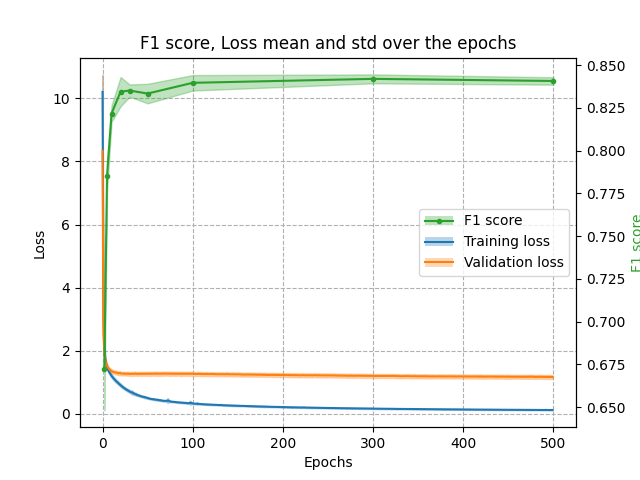
\includegraphics[scale=0.7]{Figures/results/yolov8/yolov8_xs_f1_score_and_loss.png}
    \caption{Visualisation de l'évolution du coût et du score F1 du modèle YOLOv8 xs au fil des époques.}
    \label{fig:yolov8_xs_f1_score_and_loss}
\end{figure}

\newpage

Nous observons une diminution très rapide du coût pour les ensembles d'entraînement et de validation, puis une phase très stable pour le coût des données de validation et beaucoup plus calme pour le coût des données d'entraînement qui continue de diminuer légèrement. Cela nous permet d'assumer que notre modèle est suffisamment entraîné.\\

Concernant les métriques, nous pouvons constater que le rappel et l'AP[.5] diminuent au fil des itérations après un pic, tandis que le score F1 et l'AP[.5,.05,.95] ont tendance à rester relativement stables. La précision quant à elle semble présenter une amélioration de ses résultats suite à une forte diminution de ceux-ci, mais qui reste inférieure au sommet atteint après quelques époques d'entraînement.

Comme nous pouvions nous en douter, les différentes versions affichent lors des premières itérations des différences relatives à leur taille. Néanmoins, comme nous le constatons grâce à la table \ref{tab:mean_f1_scores_yolov8_models}, retraçant les moyennes du score F1 à différentes époques pour toutes les tailles de YOLOv8, ces différences sont relativement faibles : moins de 2\%. La seule métrique où la différence est plus flagrante est l'AP[.5,.05,.95] sur la figure \ref{fig:yolov8_visulization_ap05_095_standard_models}, où nous pouvons voir que la version xs performe moins bien que celles plus grandes.

\begin{table}[!ht]
    \caption{Moyenne des scores F1 des modèles YOLOv8 à 20, 50, 100, et 500 époques}
    \label{tab:mean_f1_scores_yolov8_models}
    \rowcolors{2}{gray!25}{white}
    \centering
    \begin{tabular}{ |c||c|c|c|c|  }
        \hline
        \rowcolor{gray!50}
        Modèle & 20 & 50 & 100 & 500\\
        \hline
        YOLOv8 xs & 0.8345 & 0.8334 & 0.8397 & 0.8408\\
        YOLOv8 s & 0.8441 & 0.8457 & 0.8471 & 0.8471\\
        YOLOv8 m & 0.8520 & 0.8492 & 0.8480 & 0.8418\\
        YOLOv8 l & 0.8517 & 0.8487 & 0.8560 & 0.8443\\
        YOLOv8 xl & 0.8521 & 0.8504 & 0.8514 & 0.8435\\
        \hline
    \end{tabular}
\end{table}

De plus, les résultats des différentes versions démontrent une tendance à converger au fil de l'entraînement. En observant les moyennes des scores F1 à différentes époques de la table \ref{tab:mean_f1_scores_yolov8_models}, nous constatons que les modèles xs, et s ont tendance à continuer de s'améliorer à l'inverse des versions m, l, et xl qui performent moins bien. En observant leur déviation standard à l'aide de la table \ref{tab:std_f1_scores_yolov8_models}, il apparaît que celles des modèles xs, et s diminuent au fil des époques tandis que celle des modèles m, l, et xl augmentent. Nous pouvons supposer que les plus grandes tailles commencent à être surentraînées pendant que les plus petites continuent d'apprendre créant la tendance observée.

\begin{table}[!ht]
    \caption{Ecart-type des scores F1 des modèles YOLOv8 à 20, 50, 100, et 500 époques}
    \label{tab:std_f1_scores_yolov8_models}
    \rowcolors{2}{gray!25}{white}
    \centering
    \begin{tabular}{ |c||c|c|c|c|  }
        \hline
        \rowcolor{gray!50}
        Modèle & 20 & 50 & 100 & 500\\
        \hline
        YOLOv8 xs & 0.0086 & 0.0057 & 0.0045 & 0.0022\\
        YOLOv8 s & 0.0034 & 0.0054 & 0.0057 & 0.0016\\
        YOLOv8 m & 0.0030 & 0.0031 & 0.0035 & 0.0034\\
        YOLOv8 l & 0.0022 & 0.0034 & 0.0045 & 0.0056\\
        YOLOv8 xl & 0.0048 & 0.0048 & 0.0046 & 0.0073\\
        \hline
    \end{tabular}
\end{table}

En s'intéressant aux moyennes des différentes métriques présentées dans la table \ref{tab:max_values_for_each_metric_yolov8_models} toutes époques confondues, nous pouvons étudier plus en détail le comportement de notre modèle face au problème de la détection de jets.

La précision atteint des valeurs autour de 92\% en fonction de la version choisie. Celle-ci est plus que satisfaisante et nous indique que lorsque notre modèle détecte un élément, il s'agit très probablement d'un jet. Le rappel est quant à lui plus faible et atteint 80\%. Cette valeur bien que satisfaisante nous indique que malgré la capacité à détecter une bonne partie des jets présents sur une image, notre modèle en manque un nombre non négligeable. Le score F1 avec des valeurs supérieures à 84\%, nous indique que notre modèle est bien balancé entre les éléments qu'il détecte correctement et la totalité de ceux qu'il doit détecter.

Regardons à présent les AP[.5] et AP[.5,.05,.95]. Avec une AP[.5] au moins supérieure à 81\%, nous voyons que notre modèle est capable de réaliser d'excellentes prédictions pour une \acrshort{iou} de 50\%.

En ce qui concerne l'AP[.5,.05,.95], avec des résultats à partir de 50\%, YOLOv8 propose de bonnes prédictions. Nous pouvons comparer les performances du modèle sur notre problème de détection de jets à celui présenté par Ultralytics sur le jeu de données COCO \cite{ultralytics_detect_nodate} que nous avons reporté sur la table \ref{tab:ultralytics_yolov8_results}. En comparant les deux, nous voyons que YOLOv8 performe mieux sur la détection de jets. Cette différence est flagrante lorsque l'on compare les résultats entre les versions xs. Nous avons 37.3\% contre 50.16\%, ce qui correspond à 12.86\% d'écart. Celui-ci peut s'expliquer par le fait que l'ensemble COCO comprend énormément de classes issues d'images contenant des schémas complexes qui sont mieux appréhendés par les tailles possédant un nombre de filtres par convolution plus élevé. En gardant cela en tête, nous pouvons en déduire que pour la détection de jets, des versions d'une taille plus modeste peuvent suffire a obtenir des bonnes performances.

Nous pouvons appuyer cela par les résultats obtenus en observant la taille des modèles (disponibles dans la table \ref{tab:yolov8_flops_only_legit}), nous observons que pour vingt fois plus de paramètres et trente fois plus d'opérations, nous obtenons au maximum moins de 5\% d'écart entre les versions xs et xl.

\begin{table}[!ht]
    \caption{Valeurs moyennes maximales des métriques des modèles YOLOv8 toutes époques confondues}
    \label{tab:max_values_for_each_metric_yolov8_models}
    \rowcolors{2}{gray!25}{white}
    \centering
    \begin{tabular}{ |c||c|c|c|c|c|  }
        \hline
        \rowcolor{gray!50}
        Modèle & Précision & Rappel & Score F1 & AP[.5] & AP[.5,.05,.95]\\
        \hline
        YOLOv8 xs & 0.9200 & 0.7978 & 0.8420 & 0.8135 & 0.5016\\
        YOLOv8 s & 0.9178 & 0.8071 & 0.8478 & 0.8202 & 0.5299\\
        YOLOv8 m & 0.9148 & 0.8218 & 0.8520 & 0.8272 & 0.5403\\
        YOLOv8 l & 0.9289 & 0.8249 & 0.8560 & 0.8279 & 0.5380\\
        YOLOv8 xl & 0.9281 & 0.8185 & 0.8521 & 0.8333 & 0.5498\\
        \hline
    \end{tabular}
\end{table}

\begin{table}[!ht]
    \caption{Résultats présentés par Ultralytics pour YOLOv8 sur le jeu de données COCO}
    \label{tab:ultralytics_yolov8_results}
    \rowcolors{2}{gray!25}{white}
    \centering
    \begin{tabular}{ |c||c|  }
        \hline
        \rowcolor{gray!50}
        Modèle & AP[.5,.05,.95]\\
        \hline
        YOLOv8 xs & 0.373\\
        YOLOv8 s & 0.449\\
        YOLOv8 m & 0.502\\
        YOLOv8 l & 0.529\\
        YOLOv8 xl & 0.539\\
        \hline
    \end{tabular}
\end{table}

\clearpage

\begin{figure}[!htbp]
    \centering
    \begin{minipage}[t]{.5\textwidth}%\vspace{0pt}
      \centering
      \includegraphics[width=1.1\linewidth]{Figures/results/yolov8/precision_over_epochs_standard_sizes.png}
      \captionof{figure}{Visualisation de la précision pour les différentes tailles de YOLOv8.}
      \label{fig:yolov8_visulization_precision_standard_models}
    \end{minipage}%
    \begin{minipage}[t]{.5\textwidth}%\vspace{5pt}
      \centering
      \includegraphics[width=1.1\linewidth ]{Figures/results/yolov8/recall_over_epochs_standard_sizes.png}
      \captionof{figure}{Visualisation du rappel pour les différentes tailles de YOLOv8.}
      \label{fig:yolov8_visulization_recall_standard_models}
    \end{minipage}
\end{figure}

\begin{figure}[!htbp]
    \centering
    \begin{minipage}[t]{.5\textwidth}%\vspace{0pt}
      \centering
      \includegraphics[width=1.1\linewidth]{Figures/results/yolov8/f1_score_over_epochs_standard_sizes.png}
      \captionof{figure}{Visualisation du score F1 pour les différentes tailles de YOLOv8.}
      \label{fig:yolov8_visulization_f1_score_standard_models}
    \end{minipage}%
\end{figure}

\begin{figure}[!htbp]
    \centering
    \begin{minipage}[t]{.5\textwidth}%\vspace{0pt}
      \centering
      \includegraphics[width=1.1\linewidth]{Figures/results/yolov8/ap05_over_epochs_standard_sizes_standard_models.png}
      \captionof{figure}{Visualisation de l'AP[.5] pour les différentes tailles de YOLOv8.}
      \label{fig:yolov8_visulization_ap05_standard_models}
    \end{minipage}%
    \begin{minipage}[t]{.5\textwidth}%\vspace{5pt}
      \centering
      \includegraphics[width=1.1\linewidth ]{Figures/results/yolov8/ap05_095_over_epochs_standard_sizes_standard_models.png}
      \captionof{figure}{Visualisation de l'AP[.5,.05,.95] pour les différentes tailles de YOLOv8.}
      \label{fig:yolov8_visulization_ap05_095_standard_models}
    \end{minipage}
\end{figure}

\clearpage


%--------------------------------------
% Courbes précision x rappel
%--------------------------------------
\subsection{Résultats YOLOv8 : courbe précision-rappel}

Observons à présent la relation entre la précision et le rappel pour une \acrshort{iou} de 50\% et de 95\% respectivement sur les figures \ref{fig:yolov8_visulization_apxr05_standard_models}, et \ref{fig:yolov8_visulization_apxr095_standard_models}. La première affiche une précision relativement stable, voire diminuant très légèrement, jusqu'à un rappel d'environ 80\%, moment à partir duquel la précision chute brutalement jusqu'à 0. Cela nous indique que pour pratiquement une même précision, nous pouvons obtenir un bon rappel jusqu'à un peu moins de 80\%. Bien qu'il ne s'agisse pas d'une courbe parfaite, la relation entre la précision et le rappel est très bonne. Par ailleurs, le même comportement est observé auprès des différentes versions de YOLOv8. En effet, nous pouvons voir que la taille m débute avec une précision plus faible. Cela signifie que lors de l'inférence, le modèle a attribué le score de confiance le plus élevé à des prédictions fausses.

\begin{figure}[hbt!]
    \centering
    \includegraphics[scale=0.7]{Figures/results/yolov8/apxr_05_300.png}
    \caption{Visualisation de la moyenne des courbes précision x rappel avec un \acrshort{iou} de 0.5 pour les différentes tailles de YOLOv8 après 300 époques.}
    \label{fig:yolov8_visulization_apxr05_standard_models}
\end{figure}

Sur la deuxième figure en revanche, il ne se passe pas la même chose. La précision diminue progressivement dès un très faible rappel, puis à partir d'un seuil, différent en fonction de la taille, la précision tombe rapidement à zéro. De façon globale dès que le rappel augmente légèrement la précision est quant à elle très faible, jusqu'à un rappel de 40\% moment où toutes les précisions sont à 0.

Ce qui est intéressant est de voir que les différentes tailles n'ont pas toutes les mêmes valeurs. Nous remarquons que sur cette visualisation, la courbe du modèle xs est beaucoup plus faible que les autres. Les courbes des tailles s, l, xl ont relativement le même comportement, hormis le début de la courbe xl qui est la seule commençant à 1. La courbe de la taille m obtient quelques meilleurs résultats, mais finit tout de même par converger au même point que les courbes précédentes.

Les résultats sont évidemment moins bons sur la figure \ref{fig:yolov8_visulization_apxr095_standard_models}, car l'\acrshort{iou} est beaucoup plus élevé. Cela implique que pour qu'une détection soit validée, celle-ci doit être détectée avec beaucoup plus de précision sur l'image. Cette contrainte nous permet d'évaluer la capacité des différentes versions à gérer la précision et le rappel avec une \acrshort{iou} de 95\%.

Contrairement à la figure \ref{fig:yolov8_visulization_apxr05_standard_models} où rien ne se démarquait réellement entre les différentes tailles, nous voyons que le modèle xs a plus de mal à obtenir les mêmes résultats que les autres tailles. Cela nous permet donc de comprendre que malgré de bonnes performances dans la métrique AP[.5,.05,.95], le plus petit modèle à beaucoup plus de mal à obtenir de vraies détections avec une \acrshort{iou} d'au moins 95\%. Ainsi, si le critère principal est d'être le plus précis possible pour la zone de détection, YOLOv8 xs sera moins adaptée.

\begin{figure}[hbt!]
    \centering
    \includegraphics[scale=0.7]{Figures/results/yolov8/apxr_095_300.png}
    \caption{Visualisation de la moyenne des courbes précision x rappel avec un \acrshort{iou} de 0.95 pour les différentes tailles de YOLOv8 après 300 époques.}
    \label{fig:yolov8_visulization_apxr095_standard_models}
\end{figure}

%--------------------------------------
% Nombre de FLOPS / Vitesse
%--------------------------------------

\subsection{Résultats YOLOv8 : FLOPS et vitesse}
\label{subsec:results_yolov8_flops_vitesse}

Analysons les \acrfull{flops} et la vitesse des différentes tailles de YOLOv8 affichée sur la table \ref{tab:yolov8_flops_only_legit}.

En regardant le nombre de paramètres ou les \acrshort{flops}, nous constatons sans surprise qu'à mesure que la taille du modèle augmente, le nombre d'opérations à effectuer augmente également. En comparant les modèles xs et s dont la différence est le nombre de filtres de convolution qui est doublé, ou encore les tailles l et xl dont le nombre de filtres de convolution est 1.5 fois plus élevé. Nous constatons que la relation entre le nombre de filtres de convolution utilisés et le nombre de paramètres ou \acrshort{flops} est quadratique.

En ce qui concerne la vitesse et le nombre d'images par seconde traité par le modèle sur une carte graphique, nous observons que peu importe la taille, le temps est toujours inférieur à 1 ms et compris dans un faible intervalle. En comparant la différence de vitesse entre les tailles xs et s nous voyons que celle-ci est très faible.

Avec plus de 1500 images par secondes pour le modèle le plus grand, YOLOv8 tient ses promesses en termes de vitesse de détection et performances. Dépassant les 2000 \acrshort{fps}, les modèles xs et s se distinguent à nouveau de par leurs capacités impressionnantes pour un nombre de paramètres et d'opérations relativement faible.

\begin{table}[!ht]
    \caption{Nombre de paramètres, FLOPS, vitesse, et images par secondes pour chaque modèle de YOLOv8}
    \label{tab:yolov8_flops_only_legit}
    \rowcolors{2}{gray!25}{white}
    \centering
    \begin{tabular}{ |c||c|c|c|c| }
        \hline
        \rowcolor{gray!50}
        Modèle & Paramètres (M) & FLOPS (M) & Vitesse (ms) RTX 4070 & FPS\\
        \hline
        YOLOv8 xs & 3.225894 & 79.018728 & 0.41 & 2458\\
        YOLOv8 s & 12.856342 & 313.450472 & 0.43 & 2305\\
        YOLOv8 m & 25.665798 & 778.713192 & 0.49 & 2042\\
        YOLOv8 l & 39.401462 & 1512.913384 & 0.55 & 1806\\
        YOLOv8 xl & 61.535974 & 2362.226408 & 0.60 & 1651\\
        \hline
    \end{tabular}
\end{table}

\subsection{Résultats des versions réduites de YOLOv8 xs}

Avec les informations obtenues et déduites précédemment, et dans l'optique d'une implémentation sur \acrshort{fpga}, ou du moins, sa comparaison avec une version synthétisable pour laquelle nous avons besoin de diminuer le nombre de paramètres du modèle, nous allons observer le comportement du modèle YOLOv8 xs lorsque celui-ci est réduit. Nous allons diviser progressivement le nombre de filtres des couches de convolutions par $2$, $4$, $8$, et $16$.

Les résultats sont présentés sur les figures : \ref{fig:yolov8_visulization_precision_reduced_models}, \ref{fig:yolov8_visulization_recall_reduced_models}, \ref{fig:yolov8_visulization_f1_score_reduced_models}, \ref{fig:yolov8_visulization_ap05_reduced_models}, et \ref{fig:yolov8_visulization_ap05_095_reduced_models}, avec les mêmes métriques que pour les versions officielles de YOLOv8.

\begin{figure}[!htbp]
    \centering
    \begin{minipage}[t]{.5\textwidth}%\vspace{0pt}
      \centering
      \includegraphics[width=1.1\linewidth]{Figures/results/yolov8/precision_over_epochs_reduced_models.png}
      \captionof{figure}{Visualisation de la précision pour les versions réduites de YOLOv8 xs.}
      \label{fig:yolov8_visulization_precision_reduced_models}
    \end{minipage}%
    \begin{minipage}[t]{.5\textwidth}%\vspace{5pt}
      \centering
      \includegraphics[width=1.1\linewidth ]{Figures/results/yolov8/recall_over_epochs_reduced_models.png}
      \captionof{figure}{Visualisation du rappel pour les versions réduites de YOLOv8 xs.}
      \label{fig:yolov8_visulization_recall_reduced_models}
    \end{minipage}
\end{figure}

\begin{figure}[!htbp]
    \centering
    \begin{minipage}[t]{.5\textwidth}%\vspace{0pt}
      \centering
      \includegraphics[width=1.1\linewidth]{Figures/results/yolov8/f1_score_over_epochs_reduced_models.png}
      \captionof{figure}{Visualisation du score F1 pour les versions réduites de YOLOv8 xs.}
      \label{fig:yolov8_visulization_f1_score_reduced_models}
    \end{minipage}%
\end{figure}

\begin{figure}[!htbp]
    \centering
    \begin{minipage}[t]{.5\textwidth}%\vspace{0pt}
      \centering
      \includegraphics[width=1.1\linewidth]{Figures/results/yolov8/ap05_over_epochs_reduced_models.png}
      \captionof{figure}{Visualisation de l'AP[.5] pour les versions réduites de YOLOv8 xs.}
      \label{fig:yolov8_visulization_ap05_reduced_models}
    \end{minipage}%
    \begin{minipage}[t]{.5\textwidth}%\vspace{5pt}
      \centering
      \includegraphics[width=1.1\linewidth ]{Figures/results/yolov8/ap05_095_over_epochs_reduced_models.png}
      \captionof{figure}{Visualisation de l'AP[.5,.05,.95] pour les versions réduites de YOLOv8 xs.}
      \label{fig:yolov8_visulization_ap05_095_reduced_models}
    \end{minipage}
\end{figure}

\break

Lorsque nous regardons les diverses figures, nous constatons que la diminution des filtres impacte plus la qualité des résultats que les différences entre les modèles officiels de YOLOv8. Le rappel \ref{fig:yolov8_visulization_recall_reduced_models}, le score F1 \ref{fig:yolov8_visulization_f1_score_reduced_models}, l'AP[.5] \ref{fig:yolov8_visulization_ap05_reduced_models}, ou encore l'AP[.5,.05,.95] \ref{fig:yolov8_visulization_ap05_095_reduced_models} affichent une nette différence des résultats entre les tailles. Prenons la table \ref{tab:mean_f1_scores_yolov8_reduced_models} affichant les valeurs moyennes du score F1, nous pouvons y voir très clairement que les plus petits modèles ont besoin de plus d'époques d'entraînement pour obtenir de bonnes performances. En effet, en ayant moins de paramètres, les modèles ont plus de mal à capturer les motifs, et nécessitent plus d'entraînement afin de réussir à généraliser ce qu'ils apprennent.

Un élément venant appuyer cela, visible sur la figure \ref{fig:yolov8_visulization_f1_score_reduced_models}, et sur la table \ref{tab:std_f1_scores_yolov8_reduced_models}, concerne l'écart-type du modèle xs réduit 16 fois qui est plus élevé que pour les autres versions. Cela démontre une sensibilité du modèle dans les premières époques qui diminue au fil de l'entraînement, qui peut être dû à l'initialisation des poids, mais aussi aux données.

\begin{table}[!ht]
    \caption{Moyenne des scores F1 des modèles YOLOv8 xs réduits à 20, 50, 100, et 500 époques}
    \label{tab:mean_f1_scores_yolov8_reduced_models}
    \rowcolors{2}{gray!25}{white}
    \centering
    \begin{tabular}{ |c||c|c|c|c|  }
        \hline
        \rowcolor{gray!50}
        Modèle & 20 & 50 & 100 & 500\\
        \hline
        YOLOv8 xs reduced 16x & 0.2250 & 0.6471 & 0.7168 & 0.7564\\
        YOLOv8 xs reduced 8x & 0.7236 & 0.7870 & 0.7994 & 0.8039\\
        YOLOv8 xs reduced 4x & 0.8021 & 0.8172 & 0.8200 & 0.8071\\
        YOLOv8 xs reduced 2x & 0.8215 & 0.8258 & 0.8180  & 0.8236\\
        YOLOv8 xs & 0.8345 & 0.8334 & 0.8397 & 0.8408\\
        \hline
    \end{tabular}
\end{table}

\begin{table}[!ht]
    \caption{Ecart-type des scores F1 des modèles YOLOv8 xs réduits à 20, 50, 100, et 500 époques}
    \label{tab:std_f1_scores_yolov8_reduced_models}
    \rowcolors{2}{gray!25}{white}
    \centering
    \begin{tabular}{ |c||c|c|c|c|  }
        \hline
        \rowcolor{gray!50}
        Modèle & 20 & 50 & 100 & 500\\
        \hline
        YOLOv8 xs reduced 16x & 0.2250 & 0.0364 & 0.0245 & 0.0109\\
        YOLOv8 xs reduced 8x & 0.0253 & 0.0078 & 0.0055 & 0.0049\\
        YOLOv8 xs reduced 4x & 0.0079 & 0.0053 & 0.0061 & 0.0049\\
        YOLOv8 xs reduced 2x & 0.0020 & 0.0026 & 0.0035  & 0.0026\\
        YOLOv8 xs & 0.0107 & 0.0121 & 0.0099 & 0.0049\\
        \hline
    \end{tabular}
\end{table}

\break

Observons les valeurs moyennes maximales obtenues pour chaque métrique par nos modèles réduits. Comme visible sur la figure \ref{fig:yolov8_visulization_precision_reduced_models}, toutes les versions obtiennent des valeurs relativement proches de 90\% avec moins de 3\% de différence. Néanmoins outre cette métrique, les autres possèdent toutes un écart bien plus important. Malgré des performances relativement proches entre la taille xs et sa version divisée par 2 avec au plus 2.21\% d'écart à l'AP[.5,.05,.95], dès que les filtres de convolution sont réduits par un facteur 4 les résultats diminuent fortement.

Nous obtenons ainsi une précision entre 89 - 92\% qui est très satisfaisante. Par ailleurs, cette dernière est relativement proche de celle trouvée pour les tailles officielles de YOLOv8.

Le rappel, avec une majorité des versions autour de 75 - 79\%, est satisfaisant. Il est assez proche des modèles officiels, bien que légèrement moins performants. Pour la plus petite version, nous observons un rappel de 66\% qui est assez pauvre.

Le score F1, nous indique que la valeur la plus faible est de 75\%. Bien que celle-ci soit acceptable, nous savons grâce au score de précision et de rappel que la version la plus petite peine à détecter l'ensemble des jets sur une image. En ce qui concerne les autres, elles ont toutes un score supérieur à 80\% ce qui en font des modèles relativement bien équilibrés.

L'AP[.5] est d'au moins 74\%, nous voyons que nos modèles sont capables d'effectuer de bonnes détections. En regardant l'AP[.5,.05,.95] dont la valeur minimale est de 42.27\%, nous constatons que nos modèles ont plus de mal à réaliser des détections lorsque l'\acrshort{iou} augmente. Néanmoins, les résultats restent toujours supérieurs à ceux obtenus par YOLOv8 xs voire s sur le jeu de données COCO.\\

Comme nous pouvions nous en douter, en diminuant la taille des filtres, les performances ont également diminué. Cependant, les versions divisées par 2, 4, voire 8, présentent seulement quelques pour cent de différences par rapport aux valeurs moyennes des versions s, m, l, et xl pour la majorité des métriques. Les limitations de ces versions réduites sont en revanche notables dans les performances de l'AP[.5,.05,.95] pour lequel la différence est plus élevée.

Néanmoins, malgré la limitation des modèles réduits à détecter des éléments avec un taux d'intersection sur union très élevé, la forte réduction des paramètres et d'opérations qu'ils présentent par rapport à la faible diminution des performances en font des réseaux intéressants dans un contexte de ressources limitées.

\begin{table}[!ht]
    \caption{Valeurs moyennes maximales des métriques des modèles YOLOv8 réduits toutes époques confondues}
    \label{tab:max_values_for_each_metric_yolov8_reduced_models}
    \rowcolors{2}{gray!25}{white}
    \centering
    \begin{tabular}{ |c||c|c|c|c|c|  }
        \hline
        \rowcolor{gray!50}
        Modèle & Précision & Rappel & Score F1 & AP[.5] & AP[.5,.05,.95]\\
        \hline
        \begin{tabular}{@{}c@{}}YOLOv8 xs \\ reduced 16x\end{tabular} & 0.8943 & 0.6606 & 0.7564 & 0.7497 & 0.4227\\
        \begin{tabular}{@{}c@{}}YOLOv8 xs \\ reduced 8x\end{tabular} & 0.9008 & 0.7552 & 0.8065 & 0.7836 & 0.4481\\
        \begin{tabular}{@{}c@{}}YOLOv8 xs \\ reduced 4x\end{tabular} & 0.9055 & 0.7899 & 0.8200 & 0.8042 & 0.4695\\
        \begin{tabular}{@{}c@{}}YOLOv8 xs \\ reduced 2x\end{tabular} & 0.9200 & 0.7939 & 0.8258 & 0.8093 & 0.4795\\
        YOLOv8 xs & 0.9200 & 0.7978 & 0.8420 & 0.8135 & 0.5016\\
        \hline
    \end{tabular}
\end{table}

\clearpage

%--------------------------------------
% Precision x Recall curve
%--------------------------------------

\subsection{Résultats YOLOv8 réduit : courbe précision-rappel}

Prenons les courbes entre la précision et le rappel pour les \acrshort{iou} de 50\% et de 95\% sur les figures \ref{fig:yolov8_visulization_apxr05_reduced_models}, et \ref{fig:yolov8_visulization_apxr095_reduced_models}.

Sur la première, nous pouvons observer que les différentes versions réduites ont un comportement similaire. Nous voyons qu'elles ne démarrent pas à un, car leurs détections avec le score de confiance le plus élevé correspondent à des faux négatifs, en moyenne cela arrive plus ou moins fréquemment en fonction de la taille. La version la plus réduite diminue vers 0 légèrement plus vite que les autres modèles. Néanmoins, le comportement et les valeurs sont plutôt similaires à la courbe \ref{fig:yolov8_visulization_apxr05_standard_models} avec les modèles officiels de YOLOv8, et donc la relation entre la précision et le rappel pour une \acrshort{iou} de 50\% est très bonne.

\begin{figure}[hbt!]
    \centering
    \includegraphics[scale=0.7]{Figures/results/yolov8/apxr_05_300_reduced_models.png}
    \caption{Visualisation de la moyenne des courbes précision x rappel avec un \acrshort{iou} de 0.5 pour les différentes tailles de YOLOv8 réduites après 300 époques.}
    \label{fig:yolov8_visulization_apxr05_reduced_models}
\end{figure}

Sur la deuxième figure \ref{fig:yolov8_visulization_apxr095_reduced_models}, nous voyons que les tailles réduites performent vraiment moins bien que le modèle s qui performe lui-même moins bien que les autres versions officielles. Dans le cadre d'une \acrshort{iou} de 95\%, la relation précision rappel est très pauvre, c'est-à-dire que les modèles de plus petite taille réalisent plus de fausses détections lorsqu'il faut être plus précis sur les zones à détecter.

\begin{figure}[hbt!]
    \centering
    \includegraphics[scale=0.7]{Figures/results/yolov8/apxr_095_300_reduced_models.png}
    \caption{Visualisation de la moyenne des courbes précision x rappel avec un \acrshort{iou} de 0.5 pour les différentes tailles de YOLOv8 réduites après 300 époques.}
    \label{fig:yolov8_visulization_apxr095_reduced_models}
\end{figure}

\break

%--------------------------------------
% Nombre de FLOPS / Vitesse
%--------------------------------------

\subsection{Résultats YOLOv8 réduit : FLOPS et vitesse}

Intéressons nous au nombre de paramètres, d'opérations, ou encore la vitesse de ces versions réduites. Contrairement aux versions de YOLOv8 officielles, nous constatons que la différence de vitesse entre les différentes tailles qui varie entre 0.39 et 0.41 ms n'est pas très importante (voire négligeable étant donné l'échelle), malgré une diminution importante des opérations. Cela peut être dû à diverses raisons, par exemple : des contraintes matérielles, ou encore une parallélisation des opérations très efficaces.
Ces mesures sont à titre indicatives et sont là uniquement pour permettre d'avoir une meilleure idée de ce que le nombre de \acrshort{flops} représente.

En s'intéressant à ces derniers, nous constatons que lorsque nous divisons le nombre de filtres de convolution par 2, nous conservons le rapport quadratique avec le nombre d'opérations. Or, lorsque nous atteignons un nombre de filtres relativement faible, le nombre d'opérations arrête de suivre cette tendance. En effet, le modèle étant composé d'autres couches que des convolutions utilisant différentes tailles de filtres, nous atteignons un nombre de \acrshort{flops}, où leur présence n'est plus négligeable.

\begin{table}[!ht]
    \caption{Nombre de paramètres, FLOPS, vitesse, et images par secondes pour chaque modèle de YOLOv8 réduit}
    \label{tab:yolov8_reduced_flops_only_legit}
    \rowcolors{2}{gray!25}{white}
    \centering
    \begin{tabular}{ |c||c|c|c|c| }
        \hline
        \rowcolor{gray!50}
        Modèle & Paramètres (M) & FLOPS (M) & Vitesse (ms) RTX 4070 & FPS\\
        \hline
        \begin{tabular}{@{}c@{}}YOLOv8 xs \\ reduced 16x\end{tabular} & 0.025779 & 0.961128 & 0.39 & 2566\\
        \begin{tabular}{@{}c@{}}YOLOv8 xs \\ reduced 8x\end{tabular} & 0.0679 & 2.048744 & 0.40 & 2466\\
        \begin{tabular}{@{}c@{}}YOLOv8 xs \\ reduced 4x\end{tabular} & 0.225522 & 5.988072 & 0.39 & 2579\\
        \begin{tabular}{@{}c@{}}YOLOv8 xs \\ reduced 2x\end{tabular} & 0.834286 & 20.923112 & 0.41 & 2456\\
        YOLOv8 xs & 3.225894 & 79.018728 & 0.41 & 2458\\
        \hline
    \end{tabular}
\end{table}

\clearpage

\section{Résultats Resnet18 + Tête}

\subsection{Résultats Resnet18 + Tête pour un nombre différent de blocs de détection}

Analysons à présent les résultats obtenus avec notre implémentation de ResNet18 à laquelle nous avons ajouté une tête afin de réaliser des détections. 

Commençons par regarder l'évolution de la fonction de coût sur l'ensemble d'entraînement et de validation au fil de l'entraînement sur la figure \ref{fig:resnet18+head_loss}. Sur celle-ci, nous voyons que les deux coûts sont très proches l'un de l'autre et indiscernables sur l'image. Par ailleurs, le coût diminue plutôt rapidement avant d'atteindre une stabilité autour des cinquante premières époques. En regardant l'évolution du score F1 en parallèle, nous constatons que celui-ci atteint une valeur très élevée à la cinquantième époque et continue d'augmenter légèrement. Au bout de $500$ époques, nous observons que notre modèle n'a pas eu de grande modification de ses fonctions coûts depuis plus de $400$ époques et que son écart type est également stable. Par ailleurs, à la fin de l'entraînement, il apparaît que le score F1 évolue peu.

\begin{figure}[hbt!]
    \centering
    \includegraphics[scale=0.7]{Figures/results/resnet18+head/r18_loss.png}
    \caption{Visualisation de l'évolution du coût et du score F1 du modèle ResNet18+Tête avec 64 D.B. au fil des époques.}
    \label{fig:resnet18+head_loss}
\end{figure}

Les figures \ref{fig:resnet18+head_precision_4_nb_db}, \ref{fig:resnet18+head_recall_4_nb_db}, \ref{fig:resnet18+head_f1_score_4_nb_db}, \ref{fig:resnet18+head_ap05_4_nb_db}, et \ref{fig:resnet18+head_ap05_095_4_nb_db} représentent les moyennes des valeurs obtenues pour les différentes métriques au fil de l'entraînement. Évaluons l'impact du nombre de blocs de détections sur les performances du modèle.

\begin{figure}[!htbp]
    \centering
    \begin{minipage}[t]{.5\textwidth}%\vspace{0pt}
      \centering
      \includegraphics[width=1.1\linewidth]{Figures/results/resnet18+head/resnet18+head_precision_4_nb_db.png}
      \captionof{figure}{Visualisation de la précision de ResNet18+Tête pour un nombre différent de blocs de détection (D.B.).}
      \label{fig:resnet18+head_precision_4_nb_db}
    \end{minipage}%
    \begin{minipage}[t]{.5\textwidth}%\vspace{5pt}
      \centering
      \includegraphics[width=1.1\linewidth ]{Figures/results/resnet18+head/resnet18+head_recall_4_nb_db.png}
      \captionof{figure}{Visualisation du rappel de ResNet18+Tête pour un nombre différent de blocs de détection (D.B.).}
      \label{fig:resnet18+head_recall_4_nb_db}
    \end{minipage}
\end{figure}

\begin{figure}[!htbp]
    \centering
    \begin{minipage}[t]{.5\textwidth}%\vspace{0pt}
      \centering
      \includegraphics[width=1.1\linewidth]{Figures/results/resnet18+head/resnet18+head_f1_score_4_nb_db.png}
      \captionof{figure}{Visualisation du score F1 de ResNet18+Tête pour un nombre différent de blocs de détection (D.B.).}
      \label{fig:resnet18+head_f1_score_4_nb_db}
    \end{minipage}%
\end{figure}

\begin{figure}[!htbp]
    \centering
    \begin{minipage}[t]{.5\textwidth}%\vspace{0pt}
      \centering
      \includegraphics[width=1.1\linewidth]{Figures/results/resnet18+head/resnet18+head_ap05_4_nb_db.png}
      \captionof{figure}{Visualisation de l'AP[.5] de ResNet18+Tête pour un nombre différent de blocs de détection (D.B.).}
      \label{fig:resnet18+head_ap05_4_nb_db}
    \end{minipage}%
    \begin{minipage}[t]{.5\textwidth}%\vspace{5pt}
      \centering
      \includegraphics[width=1.1\linewidth ]{Figures/results/resnet18+head/resnet18+head_ap05_95_4_nb_db.png}
      \captionof{figure}{Visualisation de l'AP[.5,.05,.95] de ResNet18+Tête pour un nombre différent de blocs de détection (D.B.).}
      \label{fig:resnet18+head_ap05_095_4_nb_db}
    \end{minipage}
\end{figure}

\break

Un point récurrent à toutes les figures est que la version comportant 16 blocs de détections obtient de meilleurs résultats dans les premières époques d'entraînement comparé aux versions à 64 et 121 blocs, qui est également vérifiable sur les tables \ref{tab:resnet18+head_16n_metrics_avg}, \ref{tab:resnet18+head_64n_metrics_avg}, et \ref{tab:resnet18+head_121n_metrics_avg}. Cette tendance s'inverse assez rapidement, autour des trente à cinquante premières époques. Cela peut s'expliquer par le fait que chaque bloc de détection se voit attribuer beaucoup plus de jets, car le modèle travaille avec quatre à huit fois moins de blocs. Il apprend donc plus rapidement à effectuer des détections.

Cependant, chaque bloc couvrant une plus grande surface que la taille d'un jet et ne pouvant réaliser qu'une détection, ceux-ci ont plus de mal à performer lorsqu'ils doivent détecter précisément le centre d'un jet comme il est possible de l'observer sur la métrique AP@[.5:.95] avec quasiment 9\% d'écart avec la version à 64 blocs, ou encore avec la précision avec plus de 7\% de différence. En revanche, le meilleur score de rappel est obtenu par cette version plus petite, très probablement, car chaque neurone couvrant un nombre de pixels sur l'image plus élevé, il y a moins de problèmes de détection d'un même jet par deux neurones différents.\\

Plusieurs époques plus tard, les modèles comportant 64 et 121 blocs de détection obtiennent à leur tour de meilleurs résultats que la version à 16 blocs. Néanmoins, ils affichent de meilleurs résultats pour les 64 blocs. Augmenter simplement le nombre de blocs de détections ne permet donc pas d'obtenir de meilleurs résultats. Il faut donc trouver la valeur optimisant ceux-ci. Le modèle de 64 blocs va travailler sur des portions de $8 \times 8$ pixels correspondant environ au diamètre d'un jet, contrairement au modèle de 121 blocs dont la surface de travail est de $4 \times 4$. Avec une granularité trop fine, les blocs pourraient voir moins de jets lors de l'entraînement ce qui pourrait expliquer cette différence.\\

En ce qui concerne les performances, il est intéressant de voir que la version avec 64 blocs de détections est celle obtenant globalement les meilleurs résultats. Avec une précision moyenne de 85.51\%, très proche de celle avec 121 blocs, nous obtenons une précision très bonne. 

Le meilleur rappel moyen étant de 71.29, nous avons là également un rappel acceptable. Le score F1 moyen étant de 77.5\%, nous voyons que notre modèle est capable dans l'ensemble d'effectuer de bonnes détections.

Par rapport à l'AP, nous constatons que lorsque l'\acrshort{iou} est de 50\%, nous atteignons une moyenne de 68.04\%. Cette valeur nous indique que bien que le modèle arrive à effectuer des détections correctes, il reste encore de la marge pour des améliorations. Lorsque nous nous attardons sur la valeur de l'AP de 0.5 à 0.95 avec un pas de 0.05, nous voyons que nous obtenons 35.10\% ce qui est un résultat modéré. Néanmoins, cette métrique incorporant des seuils d'intersections sur union plus stricts, il n'est pas étonnant de voir qu'elle est inférieure à l'AP[.5].

\begin{table}[!ht]
    \caption{Valeurs moyenne des métriques du modèle Resnet18 + Tête avec 16 blocs de détection au fil de l'entraînement}
    \label{tab:resnet18+head_16n_metrics_avg}
    \rowcolors{2}{gray!25}{white}
    \centering
    \begin{tabular}{ |c||c|c|c|c|c|  }
        \hline
        \rowcolor{gray!50}
        Epoque & Précision & Rappel & Score F1 & AP[.5] & AP[.5,.05,.95]\\
        \hline
        2 & 0.0980 & 0.0220 & 0.0298 & 0.0079 & 0.0017\\
        5 & 0.1068 & 0.1183 & 0.1056 & 0.0264 & 0.0062\\
        10 & 0.5220 & 0.3943  & 0.4454 & 0.2512 & 0.0638\\
        20 & 0.6126 & 0.6139 & 0.6122 & 0.4201 & 0.1288\\
        30 & 0.5779 & 0.5837 & 0.5803 & 0.3923 & 0.1209\\
        50 & 0.6732 & 0.6438 & 0.6568 & 0.4851 & 0.1686\\
        100 & 0.7100 & 0.6654 & 0.6859 & 0.5277 & 0.1957\\
        300 & 0.7734 & 0.6978 & 0.7324 & 0.5928 & 0.2509\\
        500 & 0.7809 & 0.7310 & 0.7544 & 0.6250 & 0.2684\\
        \hline
    \end{tabular}
\end{table}

\begin{table}[!ht]
    \caption{Valeurs moyenne des métriques du modèle Resnet18 + Tête avec 64 blocs de détection au fil de l'entraînement}
    \label{tab:resnet18+head_64n_metrics_avg}
    \rowcolors{2}{gray!25}{white}
    \centering
    \begin{tabular}{ |c||c|c|c|c|c|  }
        \hline
        \rowcolor{gray!50}
        Epoque & Précision & Rappel & Score F1 & AP[.5] & AP[.5,.05,.95]\\
        \hline
        2 & 0.0000 & 0.0000 & 0.0000 & 0.0139 & 0.0030\\
        5 & 0.0000 & 0.0000 & 0.0000 & 0.0181 & 0.0038\\
        10 & 0.0000 & 0.0000 & 0.0000 & 0.0318 & 0.0068\\
        20 & 0.6437 & 0.5101 & 0.5666 & 0.4173 & 0.1172\\
        30 & 0.7124 & 0.5707 & 0.6308 & 0.5007 & 0.1642\\
        50 & 0.8048 & 0.6773 & 0.7339 & 0.6451 & 0.2624\\
        100 & 0.7847 & 0.7129 & 0.7441 & 0.6703 & 0.3034\\
        300 & 0.8442 & 0.7069 & 0.7676 & 0.6784 & 0.3381\\
        500 & 0.8551 & 0.7122 & 0.7750 & 0.6804 & 0.3510\\
        \hline
    \end{tabular}
\end{table}

\begin{table}[!ht]
    \caption{Valeurs moyenne des métriques du modèle Resnet18 + Tête avec 121 blocs de détection au fil de l'entraînement}
    \label{tab:resnet18+head_121n_metrics_avg}
    \rowcolors{2}{gray!25}{white}
    \centering
    \begin{tabular}{ |c||c|c|c|c|c|  }
        \hline
        \rowcolor{gray!50}
        Epoque & Précision & Rappel & Score F1 & AP[.5] & AP[.5,.05,.95]\\
        \hline
        2 & 0.0000 & 0.0000 & 0.0000 & 0.0286 & 0.0065\\
        5 & 0.0000 & 0.0000 & 0.0000 & 0.0309 & 0.0071\\
        10 & 0.0000 & 0.0000 & 0.0000 & 0.0312 & 0.0072\\
        20 & 0.1294 & 0.0013 & 0.0026 & 0.0554 & 0.0132\\
        30 & 0.5868 & 0.3869 & 0.4652 & 0.3853 & 0.0992\\
        50 & 0.8167 & 0.5682 & 0.6674 & 0.6191 & 0.2480\\
        100 & 0.8484 & 0.6264 & 0.7201 & 0.6482 & 0.2920\\
        300 & 0.8560 & 0.6690 & 0.7503 & 0.6627 & 0.3286\\
        500 & 0.8469 & 0.6832 & 0.7558 & 0.6637 & 0.3377\\
        \hline
    \end{tabular}
\end{table}

\break

Regardons à présent la courbe de la précision et du rappel pour un \acrshort{iou} de 50\% sur la figure \ref{fig:resnet18+head_apxr_05_500_4_nb_db}. Comme nous pouvions nous en douter d'après les résultats obtenus, celle-ci est loin d'être parfaite. Néanmoins, elle démontre tout de même une relation entre la précision et le rappel relativement bonne. Les versions à 64 et 121 blocs de détections s'en tirent globalement mieux, bien que le modèle à 16 blocs les rejoint lorsque le rappel augmente.

Sur la figure \ref{fig:resnet18+head_apxr_095_500_4_nb_db} en revanche, bien qu'il y ait un léger pic, les valeurs sont quasiment toujours nulles. Cela nous indique que notre modèle n'est pas capable de réaliser des détections lorsque le seuil d'intersection sur union est trop élevé.

\begin{figure}[!htbp]
    \centering
    \begin{minipage}[t]{.5\textwidth}%\vspace{0pt}
      \centering
      \includegraphics[width=1.1\linewidth]{Figures/results/resnet18+head/resnet18+head_apxr_05_500.png}
      \captionof{figure}{Visualisation de la moyenne des courbes précision x rappel avec un IoU de 0.5 pour ResNet18+Tête avec un nombre différent de blocs de détection (D.B.) après 500 époques.}
      \label{fig:resnet18+head_apxr_05_500_4_nb_db}
    \end{minipage}%
    \begin{minipage}[t]{.5\textwidth}%\vspace{5pt}
      \centering
      \includegraphics[width=1.1\linewidth ]{Figures/results/resnet18+head/resnet18+head_apxr_095_500.png}
      \captionof{figure}{Visualisation de la moyenne des courbes précision x rappel avec un IoU de 0.95 pour ResNet18+Tête avec un nombre différent de blocs de détection (D.B.) après 500 époques.}
      \label{fig:resnet18+head_apxr_095_500_4_nb_db}
    \end{minipage}
\end{figure}

\break

Finalement, observons le nombre de paramètres, d'opérations et la vitesse des différentes tailles de blocs affichés sur la table \ref{tab:resnet18+head_params_flops_vitesse_fps_4_nb_db}. Sans surprises, le nombre de blocs influe peu sur le nombre de paramètres et d'opérations du modèle.

En revanche, la vitesse d'inférence et par conséquent le nombre d'images par secondes entre la version avec 16 blocs de détection et les versions de 64 et 121 possèdent un très grand écart. A priori, étant donné que les paramètres et le nombre d'opérations sont relativement proches, il serait logique de penser que la différence ne devrait pas être très élevée. Si nous analysons le nombre d'opérations qui sont réalisées, reporté sur la table \ref{tab:resnet18+head_params_node_4_nb_db}, nous constatons que l'opération de produit matriciel (MatMul) est celle qui évolue le plus. Cette dernière uniquement présente dans les couches Dense de notre modèle explique pourquoi elle est liée au nombre de blocs utilisés. Nous pouvons donc raisonnablement supposer que le nombre de produits matriciel à effectuer à une forte incidence sur la vitesse de calcul.

Cependant, avec plus de 3900 images par seconde, et des temps inférieurs à 0.26 ms, nous voyons que les vitesses atteintes restent très élevées dans les trois cas.

\begin{table}[!ht]
    \caption{Nombre de paramètres, FLOPs, vitesse, FPS pour ResNet18+Tête avec 16, 64, et 121 blocs de détection (D.B.)}
    \label{tab:resnet18+head_params_flops_vitesse_fps_4_nb_db}
    \rowcolors{2}{gray!25}{white}
    \centering
    \begin{tabular}{ |c||c|c|c|c| }
        \hline
        \rowcolor{gray!50}
        Modèle & Paramètres (M) & MFLOPs & \begin{tabular}{@{}c@{}}Vitesse (ms) \\ RTX 4070 \end{tabular} & FPS\\
        \hline
        ResNet18+Tête 16 D.B. & 11.215536 & 287.382512 & 0.1150 & 8695\\
        ResNet18+Tête 64 D.B. & 11.289408 & 287.530112 & 0.2142 & 4668\\
        ResNet18+Tête 121 D.B. & 11.377131 & 287.705387 & 0.2508 & 3986\\
        \hline
    \end{tabular}
\end{table}

\begin{table}[!ht]
    \caption{Nombre de paramètres de chaque noeud pour ResNet18+Tête avec 16, 64, et 121 blocs de détection (D.B.)}
    \label{tab:resnet18+head_params_node_4_nb_db}
    \rowcolors{2}{gray!25}{white}
    \centering
    \begin{tabular}{ |c||c|c|c| }
        \hline
        \rowcolor{gray!50}
        Noeud & \begin{tabular}{@{}c@{}}Nb ops R18+Tête \\ 16 D.B. \end{tabular} & \begin{tabular}{@{}c@{}}Nb ops R18+Tête \\ 64 D.B. \end{tabular} & \begin{tabular}{@{}c@{}}Nb ops R18+Tête \\ 121 D.B. \end{tabular}\\
        \hline
        Conv2D & 286.95m & 286.95m & 286.95m\\
        MatMul & 49.15k & 196.61k & 371.71k\\
        BiasAdd & 194.86k & 195.01k & 195.18k\\
        MaxPool & 129.60k & 129.60k & 129.60k\\
        AddV2 & 57.47k & 57.47k & 57.47k\\
        Mean & 2.05k & 2.05k & 2.05k\\
        \hline
    \end{tabular}
\end{table}

\clearpage

\subsection{Résultats Resnet18 + Tête : versions réduites avec 64 blocs de détection}

En réduisant le nombre de filtres de convolution de notre modèle possédant 64 blocs de détection par : 2, 4, 8, 16, et 32 en vue de le synthétiser avec \acrshort{hls4ml}, nous constatons sur les figures \ref{fig:resnet18+head_precision_reduced}, \ref{fig:resnet18+head_recall_reduced}, \ref{fig:resnet18+head_f1_score_reduced}, \ref{fig:resnet18+head_ap05_reduced}, et \ref{fig:resnet18+head_ap05_095_reduced} une nette diminution des performances. Ainsi, si les versions réduites par un facteur 2, et 4 possèdent encore des résultats peu éloignés du modèle de base, les autres possèdent une différence plus marquée. Cela se comprend étant donné la diminution du nombre de paramètres, visible sur la table \ref{tab:resnet18+head_params_flops_vitesse_fps_reduced}, les modèles ont de plus en plus de mal à faire ressortir des images les schémas et les caractéristiques nécessaires à la détection des jets.\\

\begin{figure}[!htbp]
    \centering
    \begin{minipage}[t]{.5\textwidth}%\vspace{0pt}
      \centering
      \includegraphics[width=1\linewidth]{Figures/results/resnet18+head/r18+h_precision_over_epochs_reduced_models.png}
      \captionof{figure}{Visualisation de la précision de ResNet18+Tête avec 64 blocs de détection (D.B.) pour les versions réduites.}
      \label{fig:resnet18+head_precision_reduced}
    \end{minipage}%
    \begin{minipage}[t]{.5\textwidth}%\vspace{5pt}
      \centering
      \includegraphics[width=1\linewidth ]{Figures/results/resnet18+head/r18+h_recall_over_epochs_reduced_models.png}
      \captionof{figure}{Visualisation du rappel de ResNet18+Tête avec 64 blocs de détection (D.B.) pour les versions réduites.}
      \label{fig:resnet18+head_recall_reduced}
    \end{minipage}
\end{figure}

\begin{figure}[!htbp]
    \centering
    \begin{minipage}[t]{.5\textwidth}%\vspace{0pt}
      \centering
      \includegraphics[width=1\linewidth]{Figures/results/resnet18+head/r18+h_f1_score_over_epochs_reduced_models.png}
      \captionof{figure}{Visualisation du score F1 de ResNet18+Tête avec 64 blocs de détection (D.B.) pour les versions réduites.}
      \label{fig:resnet18+head_f1_score_reduced}
    \end{minipage}%
\end{figure}

\begin{figure}[!htbp]
    \centering
    \begin{minipage}[t]{.5\textwidth}%\vspace{0pt}
      \centering
      \includegraphics[width=1\linewidth]{Figures/results/resnet18+head/r18+h_ap05_over_epochs_reduced_models.png}
      \captionof{figure}{Visualisation de l'AP[.5] de ResNet18+Tête avec 64 blocs de détection (D.B.) pour les versions réduites.}
      \label{fig:resnet18+head_ap05_reduced}
    \end{minipage}%
    \begin{minipage}[t]{.5\textwidth}%\vspace{5pt}
      \centering
      \includegraphics[width=1\linewidth ]{Figures/results/resnet18+head/r18+h_ap05_095_over_epochs_reduced_models.png}
      \captionof{figure}{Visualisation de l'AP[.5,.05,.95] de ResNet18+Tête avec 64 blocs de détection (D.B.) pour les versions réduites.}
      \label{fig:resnet18+head_ap05_095_reduced}
    \end{minipage}
\end{figure}

\break

Au niveau des performances, la table \ref{tab:max_values_for_each_metric_resnet18+head_reduced_models} nous montre les valeurs moyennes maximales toutes époques confondues pour les différentes métriques. Sur celle-ci, nous voyons que la diminution du nombre de filtres des couches de convolutions à un impact très important sur les résultats obtenus. En observant la différence entre le modèle de base et celui divisé par deux, nous observons entre 2 et 6\% d'écart, qui s'étend entre 9 et 13\% pour une division par quatre. Ce dernier, avec un score F1 de 69.82\% et une AP[.5] de 59.28\% qui sont des valeurs potentiellement acceptables, n'obtient que 22.37\% en moyenne pour l'AP[.5,.05,.95] qui est un score très pauvre.

Les versions encore plus petites obtiennent des valeurs encore plus faibles, démontrant les limites du modèle lorsque nous le réduisons.

\begin{table}[!ht]
    \caption{Valeurs moyennes maximales des métriques du modèle ResNet18+Tête avec 64 blocs de détection (D.B.) réduit toutes époques confondues}
    \label{tab:max_values_for_each_metric_resnet18+head_reduced_models}
    \rowcolors{2}{gray!25}{white}
    \centering
    \begin{tabular}{ |c||c|c|c|c|c|  }
        \hline
        \rowcolor{gray!50}
        Modèle & Précision & Rappel & Score F1 & AP[.5] & AP[.5,.05,.95]\\
        \hline
        R18+Tête 64 D.B & 0.8551 & 0.7129 & 0.7750 & 0.6804 & 0.3510\\
        R18+Tête 64 D.B. r. 2x & 0.8216 & 0.6795 & 0.7429 & 0.6409 & 0.2964\\
        R18+Tête 64 D.B. r. 4x & 0.7619 & 0.6446 & 0.6982 & 0.5928 & 0.2237\\
        R18+Tête 64 D.B. r. 8x & 0.6834 & 0.5186 & 0.5845 & 0.4785 & 0.1624\\
        R18+Tête 64 D.B. r. 16x & 0.5622 & 0.3828 & 0.4515 & 0.3129 & 0.0825\\
        R18+Tête 64 D.B. r. 32x & 0.4356 & 0.2322 & 0.2981 & 0.1607  & 0.0365\\
        \hline
    \end{tabular}
\end{table}

Au niveau de la courbe précision et rappel, celle-ci nous laisse voir sur la figure \ref{fig:resnet18+head_apxr_05_500_reduced} pour une \acrshort{iou} de 50\% que la version de base ainsi que celles réduites par deux, et quatre sont relativement proches. Puis les modèles encore plus réduits possèdent, à leur niveau, une relation plus pauvre. En regardant la même courbe pour une \acrshort{iou} de 95\% sur la figure \ref{fig:resnet18+head_apxr_095_500_reduced}, nous voyons que celle-ci est quasi nulle.

\begin{figure}[!htbp]
    \centering
    \begin{minipage}[t]{.5\textwidth}%\vspace{0pt}
      \centering
      \includegraphics[width=1\linewidth]{Figures/results/resnet18+head/r18+h_apxr_05_500_reduced_models.png}
      \captionof{figure}{Visualisation de la moyenne des courbes précision x rappel avec un IoU de 0.5 pour les versions réduites de ResNet18+Tête avec 64 blocs de détection (D.B.) après 500 époques.}
      \label{fig:resnet18+head_apxr_05_500_reduced}
    \end{minipage}%
    \begin{minipage}[t]{.5\textwidth}%\vspace{5pt}
      \centering
      \includegraphics[width=1\linewidth ]{Figures/results/resnet18+head/r18+h_apxr_095_500_reduced_models.png}
      \captionof{figure}{Visualisation de la moyenne des courbes précision x rappel avec un IoU de 0.95 pour les versions réduites de ResNet18+Tête avec 64 blocs de détection (D.B.) après 500 époques.}
      \label{fig:resnet18+head_apxr_095_500_reduced}
    \end{minipage}
\end{figure}

\break

Bien que le modèle de base performe relativement bien, la réduction des filtres des couches de convolution est mal supportée par le modèle. Cependant en gardant en tête qu'il s'agit de base d'un modèle de classification que nous avons détourné pour en faire un modèle de détection en utilisant une tête très simple, celui-ci fonctionne plutôt bien.\\

Finalement, sur la table \ref{tab:resnet18+head_params_flops_vitesse_fps_reduced} nous retrouvons à nouveau une relation quadratique entre les différentes versions de ResNet18+Tête. Cela est vrai jusqu'à un certain facteur à partir duquel les paramètres d'autres couches deviennent significatifs.

En ce qui concerne la vitesse, nous observons un gain lors des premières réductions des filtres qui se stabilise par la suite. Le nombre de blocs de détection reste constant et comme nous l'avons vu précédemment, celui-ci influence la vitesse d'inférence du modèle. Nous supposons alors que malgré une forte diminution du nombre de paramètres et d'opérations, le modèle atteint ses limites, du moins sur la carte graphique utilisée, à cause du nombre de blocs de détection. À titre de comparaison, en travaillant avec ResNet18+Tête avec 16 blocs de détections et dont le nombre de filtres a été divisé par 16, nous obtenons un temps d'inférence de 0.093 ms ce qui donne 10748 images par secondes. La différence entre cette version réduite et celle non réduite est de plus de 2000 images par seconde contrairement à la version avec 64 blocs de détections dont l'écart est de moins de 600 images par secondes.

Néanmoins, dépassant rapidement les 5000 images par seconde avec un temps d'inférence inférieur à 0.2 ms, nous constatons que les variantes de notre modèle, avec des performances mitigées, sont capables de vitesses très intéressantes dans le cadre d'applications en temps réel.

\begin{table}[!ht]
    \caption{Nombre de paramètres, FLOPs, vitesse, FPS pour ResNet18+Tête avec 16, 64, et 121 blocs de détection (D.B)}
    \label{tab:resnet18+head_params_flops_vitesse_fps_reduced}
    \rowcolors{2}{gray!25}{white}
    \centering
    \begin{tabular}{ |c||c|c|c|c| }
        \hline
        \rowcolor{gray!50}
        Modèle & Paramètres (M) & MFLOPs & Vitesse (ms) RTX 4070 & FPS\\
        \hline
        R18+Tête 64 D.B. & 11.289408 & 287.530112 & 0.2142 & 4668\\
        R18+Tête 64 D.B. r. 2x & 2.855424 & 76.844704 & 0.2016 & 4960\\
        R18+Tête 64 D.B. r. 4x & 0.730464 & 21.692336 & 0.1974 & 5066\\
        R18+Tête 64 D.B. r. 8x & 0.190992 & 6.663736 & 0.1933 & 5171\\
        R18+Tête 64 D.B. r. 16x & 0.052008 & 2.286332 & 0.1920 & 5208\\
        R18+Tête 64 D.B. r. 32x & 0.015204 & 0.881854 & 0.1937 & 5161\\
        \hline
    \end{tabular}
\end{table}

\break

\subsection{Résultats ResNet18+Tête : version quantifiée avec 64 blocs de détection}

Étant donné que nous souhaitons synthétiser notre modèle ResNet18+Tête à l'aide de HLS4ML en vue d'une implémentation sur \acrshort{fpga}, nous avons d'abord quantifié ce dernier à l'aide de QKeras afin d'obtenir le réseau de neurones le plus proche du résultat final.

Notre version fraîchement quantifiée de ResNet18+Tête avec 64 blocs de détection est malheureusement plus lente en termes de vitesse de calculs. Cela est notamment dû au fait qu'elle n'arrive pas à profiter des unités de calculs de la carte graphique destinées aux virgules flottantes, car elle utilise une représentation en virgule fixe. Afin de gagner du temps, il est possible de réaliser de l'apprentissage par transfert en utilisant les poids du modèle à virgule flottante comme base afin d'accélérer l'entraînement, plutôt que d'en réaliser un nouveau à partir de poids initialisé aléatoirement.\\

Les figures \ref{fig:qresnet18+head_precision}, \ref{fig:qresnet18+head_recall}, \ref{fig:qresnet18+head_f1_score}, \ref{fig:qresnet18+head_ap05}, \ref{fig:qresnet18+head_ap05_095}, \ref{fig:qresnet18+head_apxr_05_500}, et \ref{fig:qresnet18+head_apxr_095_500} nous permettent de voir l'évolution du modèle pour nos différentes métriques au fil des $500$ premières époques de l'entraînement de la version de base, ainsi que de ses alternatives quantifiées sur 8 et 16 bits réutilisant des poids, ou à partir de zéro. Ces dernières ont été entraînées sur mille époques, mais pour des soucis de visibilité sur les figures elles ne seront pas représentées. Néanmoins, leurs résultats sont accessibles aux tables \ref{appendix:qresnet18_8b_fs}, et \ref{appendix:qresnet18_8b_fs} en annexes.

\begin{figure}[!htbp]
    \centering
    \begin{minipage}[t]{.5\textwidth}%\vspace{0pt}
      \centering
      \includegraphics[width=1.1\linewidth]{Figures/results/qresnet18+head/qr18+h_precision_over_epochs_500.png}
      \captionof{figure}{Visualisation de la précision de ResNet18+Tête avec 64 blocs de détection (D.B.) et ses versions quantifiées de 8 et 16 bits.}
      \label{fig:qresnet18+head_precision}
    \end{minipage}%
    \begin{minipage}[t]{.5\textwidth}%\vspace{5pt}
      \centering
      \includegraphics[width=1.1\linewidth ]{Figures/results/qresnet18+head/qr18+h_rappel_over_epochs_500.png}
      \captionof{figure}{Visualisation du rappel de ResNet18+Tête avec 64 blocs de détection (D.B.) et ses versions quantifiées de 8 et 16 bits.}
      \label{fig:qresnet18+head_recall}
    \end{minipage}
\end{figure}

\begin{figure}[!htbp]
    \centering
    \begin{minipage}[t]{.5\textwidth}%\vspace{0pt}
      \centering
      \includegraphics[width=1.1\linewidth]{Figures/results/qresnet18+head/qr18+h_f1_score_over_epochs_500.png}
      \captionof{figure}{Visualisation du score F1 de ResNet18+Tête avec 64 blocs de détection (D.B.) et ses versions quantifiées de 8 et 16 bits.}
      \label{fig:qresnet18+head_f1_score}
    \end{minipage}%
\end{figure}

\begin{figure}[!htbp]
    \centering
    \begin{minipage}[t]{.5\textwidth}%\vspace{0pt}
      \centering
      \includegraphics[width=1.1\linewidth]{Figures/results/qresnet18+head/qr18+h_ap05_over_epochs_500.png}
      \captionof{figure}{Visualisation de l'AP[.5] de ResNet18+Tête avec 64 blocs de détection (D.B.) et ses versions quantifiées de 8 et 16 bits.}
      \label{fig:qresnet18+head_ap05}
    \end{minipage}%
    \begin{minipage}[t]{.5\textwidth}%\vspace{5pt}
      \centering
      \includegraphics[width=1.1\linewidth ]{Figures/results/qresnet18+head/qr18+h_ap05_095_over_epochs_500.png}
      \captionof{figure}{Visualisation de l'AP[.5,.05,.95] de ResNet18+Tête avec 64 blocs de détection (D.B.) et ses versions quantifiées de 8 et 16 bits.}
      \label{fig:qresnet18+head_ap05_095}
    \end{minipage}
\end{figure}

\break

Lorsque nous observons les différentes figures, nous constatons effectivement qu'à partir des poids initialisés aléatoirement les versions quantifiées sur 8 et 16 bits nécessitent plus d'époques d'entraînement pour atteindre des performances similaires. En réutilisant les poids des versions à virgules flottantes, nous voyons qu'il faut effectivement peu d'époques pour atteindre en moyenne des résultats similaires. Cependant, un point intéressant à relever est l'écart type qui est plus élevé sur les modèles réutilisant des poids que sur ceux apprenant à partir de zéro.

Cela est très certainement dû aux poids optimisés pour une représentation à virgule flottante. La perte de précision générée par la quantification demande au modèle d'affiner ses poids dans une résolution à virgule fixe. Celui-ci doit s'adapter à une nouvelle représentation introduisant alors une certaine instabilité. À l'inverse, lors d'un entraînement depuis le début, le modèle va s'adapter plus progressivement et, comme nous pouvons le voir sur les figures, sera plus stable.\\

Bien qu'il y ait quelques pour cent d'écart, les figures nous montrent que les différentes versions évoluent vers des résultats plutôt proches. Au niveau des différentes métriques, nous voyons qu'elles ont toutes des résultats relativement proches. Cependant, bien que cela ne soit pas visible sur la figure affichant la précision, le modèle le plus performant reste la version à virgule flottante, et le moins bon semble être la version quantifiée sur 8 bits entraînés à partir de zéro. Les autres versions sont plus complexes à analyser sur les figures, nous étudierons leur comportement plus loin avec les valeurs moyennes maximales.\\

En ce qui concerne la relation de la précision avec le rappel pour une \acrshort{iou} de 50\%, nous voyons sur la figure \ref{fig:qresnet18+head_apxr_05_500}, que le comportement est relativement similaire à celui du modèle de base, avec une légère baisse de la qualité de la précision en fonction du rappel. Il reste néanmoins très bon.

Avec une \acrshort{iou} de 95\% sur la figure \ref{fig:qresnet18+head_apxr_095_500}, nous voyons que celle-ci est toujours aussi mauvaise pour la version quantifiée sur 16 bits, mais surprenamment, bien que le modèle quantifié sur 8 bits soit également mauvais, il semble performer mieux lors d'un très faible rappel. Il est possible qu'avec une représentation sur 8 bits le modèle arrive à mieux généraliser ce qui lui confère de légères meilleures performances lors d'une intersection sur union plus élevée. Néanmoins, malgré les pauvres résultats obtenus sur cette courbe, nous voyons que les versions quantifiées s'en tirent au moins aussi bien que celle de base.\\

\begin{figure}[!htbp]
    \centering
    \begin{minipage}[t]{.5\textwidth}%\vspace{0pt}
      \centering
      \includegraphics[width=1.1\linewidth]{Figures/results/qresnet18+head/qr18+h_apxr_05_500.png}
      \captionof{figure}{Visualisation de la moyenne des courbes précision x rappel avec un IoU de 0.5 pour les versions quantifiées de 8 et 16 bits de ResNet18+Tête avec 64 blocs de détection (D.B.) après 500 époques.}
      \label{fig:qresnet18+head_apxr_05_500}
    \end{minipage}%
    \begin{minipage}[t]{.5\textwidth}%\vspace{5pt}
      \centering
      \includegraphics[width=1.1\linewidth ]{Figures/results/qresnet18+head/qr18+h_apxr_05_095_500.png}
      \captionof{figure}{Visualisation de la moyenne des courbes précision x rappel avec un IoU de 0.95 pour les versions quantifiées de 8 et 16 bits de ResNet18+Tête avec 64 blocs de détection (D.B.) après 500 époques.}
      \label{fig:qresnet18+head_apxr_095_500}
    \end{minipage}
\end{figure}

Analysons à présent les valeurs moyennes maximums de chaque version pour chaque métrique toutes époques confondues disponibles sur la table \ref{tab:max_values_for_each_metric_qresnet18+head_models}. Nous voyons que les versions quantifiées obtiennent des performances relativement proches du modèle à représentation en virgule flottante. Entre les différentes versions, il n'y a que quelques pourcentages de différence à travers toutes les métriques. Cependant, le modèle sur 8 bits performe légèrement moins bien que celui sur 16 bits dans toutes les métriques excepté la précision. Ce dernier possède des valeurs relativement proches, voire équivalentes au modèle de base, bien que sur l'AP[.5,.05,.95], nous observons une plus grosse différence.

De plus, la différence entre les versions quantifiées pré-entrainées et celles entraînées de zéro est très faible alors que ces dernières affichent des valeurs tirées parmi les résultats au bout de plus de $500$ époques, confirmant à nouveau que l'utilisation de poids à virgule flottante pré-entraînés accélère l'entraînement des versions quantifiées.

Ainsi, avec un score F1 de 77.14\%, une AP[.5] de 68\%, et une AP[.5,.05,.95] de 32\%, la version quantifiée de ResNet18+Tête sur 16 bits présente des performances quasi identiques au modèle de base, qui sont relativement bonnes. C'est cette version que nous allons ajuster et utiliser avec le paquet HLS4ML.

\begin{table}[!ht]
    \caption{Valeurs moyennes maximales des métriques du modèle ResNet18+Tête avec 64 blocs de détection (D.B.) quantifié sur 8 ou 16 bits à partir de poids préentrainés sur un modèle à virgule flottante et à partir de zéro}
    \label{tab:max_values_for_each_metric_qresnet18+head_models}
    \rowcolors{2}{gray!25}{white}
    \centering
    \begin{tabular}{ |c||c|c|c|c|c|  }
        \hline
        \rowcolor{gray!50}
        Modèle & Précision & Rappel & Score F1 & AP[.5] & AP[.5,.05,.95]\\
        \hline
        R18+Tête 64 D.B & 0.8551 & 0.7129 & 0.7750 & 0.6804 & 0.3510\\
        \begin{tabular}{@{}c@{}}QR18+Tête 64 D.B. \\ 8 bits pré-entrainé\end{tabular} & 0.8512 & 0.7134 & 0.7677 & 0.6687 & 0.3200\\
        \begin{tabular}{@{}c@{}}QR18+Tête 64 D.B. \\ 8 bits de zéro\end{tabular} & 0.8360 & 0.6963 & 0.7582 & 0.6683 & 0.3031\\
        \begin{tabular}{@{}c@{}}QR18+Tête 64 D.B. \\ 16 bits pré-entrainé\end{tabular} & 0.8473 & 0.7258 & 0.7714 & 0.6830 & 0.3231\\
        \begin{tabular}{@{}c@{}}QR18+Tête 64 D.B. \\ 16 bits de zéro\end{tabular} & 0.8551 & 0.7131 & 0.7769 & 0.6616 & 0.3387\\
        \hline
    \end{tabular}
\end{table}

\subsection{Résultats ResNet18+Tête : version quantifiée pour HLS4ML}

Comme nous avons pu le voir précédemment, la version de notre modèle quantifié sur 16 bits semble être adaptée pour notre cas. Afin de pouvoir l'utiliser avec HLS4ML, nous avons dû réduire la taille de celui-ci afin de permettre à l'outil d'optimiser la latence. Pour cela, nous avons décidé d'utiliser la version réduisant le nombre de filtres par convolution par seize. Malgré ses maigres performances, celui-ci nous permet de maximiser le nombre de couches utilisant la stratégie "latence", tout en limitant les ressources matérielles nécessaires pour aboutir à la synthèse.

Cependant, HLS4ML ne supporte malheureusement pas l'utilisation de stride dans la couche de MaxPooling. Afin de pouvoir tout de même synthétiser notre modèle, nous avons retiré ce stride.\\

Cette sous-section a donc pour but de présenter les performances de la version quantifiée puis synthétisée avec HLS4ML. Les figures \ref{fig:qresnet18+head_precision_wo_stride}, \ref{fig:qresnet18+head_recall_wo_stride}, \ref{fig:qresnet18+head_f1_score_wo_stride}, \ref{fig:qresnet18+head_ap05_wo_stride}, \ref{fig:qresnet18+head_ap05_095_wo_stride}, \ref{fig:qresnet18+head_apxr_05_500_wo_stride}, et \ref{fig:qresnet18+head_apxr_095_500_wo_stride} affichent les résultats de la version de base dont les filtres de convolution ont été réduits seize fois, ainsi que sa version quantifiée aux côtés des mêmes modèles dont le stride à la couche MaxPooling a été retirée. L'entraînement des versions quantifiées a été réalisé à partir des poids des versions à virgule flottante.

\begin{figure}[!htbp]
    \centering
    \begin{minipage}[t]{.5\textwidth}%\vspace{0pt}
      \centering
      \includegraphics[width=1.1\linewidth]{Figures/results/qresnet18+head/qr18+h_precision_over_epochs_500_wo_stride.png}
      \captionof{figure}{Visualisation de la précision de ResNet18+Tête avec 64 blocs de détection (D.B.) pour sa version quantifiée sur 16 bits réduite 16 fois avec et sans MaxPooling stride.}
      \label{fig:qresnet18+head_precision_wo_stride}
    \end{minipage}%
    \begin{minipage}[t]{.5\textwidth}%\vspace{5pt}
      \centering
      \includegraphics[width=1.1\linewidth ]{Figures/results/qresnet18+head/qr18+h_rappel_over_epochs_500_wo_stride.png}
      \captionof{figure}{Visualisation du rappel de ResNet18+Tête avec 64 blocs de détection (D.B.) pour sa version quantifiée sur 16 bits réduite 16 fois avec et sans MaxPooling stride.}
      \label{fig:qresnet18+head_recall_wo_stride}
    \end{minipage}
\end{figure}

\begin{figure}[!htbp]
    \centering
    \begin{minipage}[t]{.5\textwidth}%\vspace{0pt}
      \centering
      \includegraphics[width=1.1\linewidth]{Figures/results/qresnet18+head/qr18+h_f1_score_over_epochs_500_wo_stride.png}
      \captionof{figure}{Visualisation du score F1 de ResNet18+Tête avec 64 blocs de détection (D.B.) pour sa version quantifiée sur 16 bits réduite 16 fois avec et sans MaxPooling stride.}
      \label{fig:qresnet18+head_f1_score_wo_stride}
    \end{minipage}%
\end{figure}

\begin{figure}[!htbp]
    \centering
    \begin{minipage}[t]{.5\textwidth}%\vspace{0pt}
      \centering
      \includegraphics[width=1.1\linewidth]{Figures/results/qresnet18+head/qr18+h_precision_over_epochs_500_wo_stride.png}
      \captionof{figure}{Visualisation de l'AP[.5] de ResNet18+Tête avec 64 blocs de détection (D.B.) pour sa version quantifiée sur 16 bits réduite 16 fois avec et sans MaxPooling stride.}
      \label{fig:qresnet18+head_ap05_wo_stride}
    \end{minipage}%
    \begin{minipage}[t]{.5\textwidth}%\vspace{5pt}
      \centering
      \includegraphics[width=1.1\linewidth ]{Figures/results/qresnet18+head/qr18+h_ap05_095_over_epochs_500_wo_stride.png}
      \captionof{figure}{Visualisation de l'AP[.5,.05,.95] de ResNet18+Tête avec 64 blocs de détection (D.B.) pour sa version quantifiée sur 16 bits réduite 16 fois avec et sans MaxPooling stride.}
      \label{fig:qresnet18+head_ap05_095_wo_stride}
    \end{minipage}
\end{figure}

\break

Nous remarquons immédiatement la perte de performances entre les versions à représentation flottante et fixe. De plus, nous constatons également une diminution des résultats pour les versions n'utilisant pas de stride. Cependant, il est intéressant de noter que cette différence est plus prononcée pour les versions à virgule flottante que celles à virgule fixe. Finalement, tout comme pour les variantes de ResNet18+Tête réalisées, nous voyons sur les courbes de précisions et de rappel que lors d'une intersection sur union de 50\% sur la figure \ref{fig:qresnet18+head_apxr_05_500_wo_stride}, même si celle-ci est pauvre, elle demeure capable d'obtenir une certaine précision tant que le rappel n'est pas trop élevé. En revanche, dès que l'\acrshort{iou} passe à 95\%, la courbe est inexistante, comme visible sur la figure \ref{fig:qresnet18+head_apxr_095_500_wo_stride}.

\begin{figure}[!htbp]
    \centering
    \begin{minipage}[t]{.5\textwidth}%\vspace{0pt}
      \centering
      \includegraphics[width=1.1\linewidth]{Figures/results/qresnet18+head/qr18+h_apxr_05_500_wo_stride.png}
      \captionof{figure}{Visualisation de la moyenne des courbes précision x rappel avec un IoU de 0.5 pour la version quantifiée sur 16 bits avec et sans MaxPooling stride de ResNet18+Tête avec 64 blocs de détection (D.B.) réduite 16 fois après 500 époques.}
      \label{fig:qresnet18+head_apxr_05_500_wo_stride}
    \end{minipage}%
    \begin{minipage}[t]{.5\textwidth}%\vspace{5pt}
      \centering
      \includegraphics[width=1.1\linewidth ]{Figures/results/qresnet18+head/qr18+h_apxr_05_095_500_wo_stride.png}
      \captionof{figure}{Visualisation de la moyenne des courbes précision x rappel avec un IoU de 0.95 pour la version quantifiée sur 16 bits avec et sans MaxPooling stride de ResNet18+Tête avec 64 blocs de détection (D.B.) réduite 16 fois après 500 époques.}
      \label{fig:qresnet18+head_apxr_095_500_wo_stride}
    \end{minipage}
\end{figure}

\break

Retirer le stride à la couche de MaxPooling à plusieurs impacts. Celui-ci sert notamment à réduire la dimensionnalité de l'entrée de la couche permettant de mieux capturer les caractéristiques et de réduire les informations non pertinentes, telles que le bruit. Mais, il permet également de réduire le nombre de calculs à réaliser par la suite.

Même si la différence entre les versions quantifiées n'est pas très importante, il est dommage de perdre ces pourcentages lors de l'étape de synthèse. Cependant, afin de pouvoir aboutir à un résultat, nous allons utiliser cette version sans stride.

\section{Comparaison des résultats entre YOLOv8 et Resnet18 + Tête}

Comparons à présent les deux modèles utilisés dans ce travail. Sans surprises, YOLOv8, le modèle développé pour effectuer de la détection d'objets performe sans aucun doute mieux que la version ResNet18+Tête en termes de précision, rappel, score F1, et précision moyenne. Avec des résultats élevés et une faculté à réaliser des détections même avec de grandes contraintes d'intersection sur union, il ne fait aucun doute que YOLOv8 est un modèle très puissant et plus que capable de réaliser la détection de jets. De plus, comme nous avons pu le voir, même les versions réduites de celui-ci sont capables d'obtenir des résultats corrects avec une perte de performances acceptable.

De l'autre côté, bien que moins performant, ResNet18+Tête démontre qu'un modèle de classification modifié pour réaliser de la détection est également capable d'obtenir des résultats satisfaisants. Cependant, contrairement à YOLOv8, ce dernier supporte moins bien la réduction du nombre de filtres de ses couches de convolution, dégradant assez fortement ses performances. Néanmoins, ResNet18+Tête se démarque face à YOLOv8, notamment au niveau de la vitesse qu'il est capable d'atteindre, mais aussi de par son implémentation plus simple qui permet de facilement le modifier, notamment afin de l'adapter à son utilisation avec HLS4ML.

Ainsi, malgré les performances plus élevées avec le modèle YOLOv8, les limitations rencontrées avec \acrshort{hls4ml} font de ResNet18+Tête un choix intéressant dans des contraintes de performances en temps réel très exigeantes.

\section{Synthèse du modèle réduit QResnet18+Tête avec HLS4ML}

Afin de synthétiser notre modèle avec HLS4ML, nous avons dû installer l'outil Vitis HLS. Pour des raisons d'espace mémoire sur la machine utilisée, nous avons utilisé la version 2022.1. Celle-ci inclut par défaut plusieurs types de \acrshort{fpga}. Cependant, de par la taille de notre réseau de neurones, nous souhaitons synthétiser notre code pour le modèle U250 \cite{noauthor_alveo_nodate} de la famille Alveo. Ces cartes ont été développées afin de répondre aux besoins des centres de données, et proposent de meilleures performances que les processeurs notamment dans le domaine de l'inférence de modèles de machine learning. La carte utilisée possède 5376 \acrfull{bram}, 12288 \acrfull{dsp}, 3456000 \acrfull{ff}, et 1728000 \acrfull{lut}. De plus, les cycles d'horloges de notre projet ont été laissés à la valeur par défaut, c'est-à-dire $5 \: ns$.

Lorsque nous synthétisons notre modèle avec HLS4ML, le paquet va créer un dossier contenant tous les éléments qu'il a générés. Parmi ceux-ci, nous retrouvons le code VHDL, Verilog, ainsi qu'un dossier nommé "report" contenant des fichiers .rpt donnant les détails de chaque couche synthétisée, comme la latence, le nombre de ressources utilisées, etc.. Parmi ces fichiers, nous retrouvons un résumé de la totalité du modèle.\\

La version synthétisée, QResNet18+Tête sans MaxPooling stride divisée par 16, nous affiche les résultats présentés sur la table \ref{tab:resources_and_latency_by_reuse_factor}. Nous pouvons voir sur celle-ci des valeurs différentes en fonction du "reuse factor" utilisé pour 1, 10, 100, et 1000. Celui-ci permet d'indiquer à l'outil le nombre de fois qu'un bloc de calcul doit être réutilisé.

Ainsi, nous voyons que le nombre de \acrshort{dsp} diminue lorsque nous augmentons le nombre de réutilisations. Cependant, diminuer le nombre de \acrshort{dsp} augmente la latence de notre système. Cela est logique étant donné qu'attribuer un "reuse factor" de $1$, revient à paralléliser l'ensemble des opérations à effectuer, mais demande un nombre de ressources très conséquentes. Comme nous pouvons le voir sur la table, ne pas réutiliser de \acrshort{dsp} demande l'utilisation d'un nombre trop élevé de ces derniers. Synthétiser notre modèle demande donc de trouver le subtil équilibre entre la parallélisation des calculs et les ressources à disposition, en acceptant d'augmenter la latence.

Par ailleurs, nous constatons que lorsque nous diminuons le nombre de \acrshort{dsp}, nous augmentons le nombre de \acrshort{ff}, et de \acrshort{lut} utilisés. En effet, les \acrshort{ff} vont permettre de temporiser les calculs qui doivent être effectués par un nombre plus restreint de \acrshort{dsp}, tandis que les \acrshort{lut} vont pouvoir réaliser des fonctions relativement simples.\\

Une autre mesure est l'\acrfull{ii}, qui indique le nombre de cycles d'horloges (\acrfull{cc}) requis avant que l'algorithme accepte une nouvelle entrée. Comme nous pouvons le constater, celle-ci est relativement proche de la latence lorsque le "reuse factor" est plutôt faible. Cependant, lorsque celui-ci augmente et devient assez grand comme pour le cas à $1000$, nous remarquons que l'\acrshort{ii} peut indiquer un temps beaucoup plus court que la latence. Ceci peut s'expliquer de par le fait que les opérations sont pipelinées efficacement aux côtés d'une conception traitant les entrées par étapes plutôt que parallèlement.

Le "reuse factor" de $1000$ a donc une latence plus élevée, mais propose dans le meilleur des cas un débit plus élevé que les versions pour lesquelles le "reuse factor" est de $100$ ou de $10$.\\

Finalement, à l'aide de notre table \ref{tab:resources_and_latency_by_reuse_factor}, nous voyons qu'utiliser un "reuse factor" de 10 permet de synthétiser notre modèle sur l'U250 avec une latence de 0.167 ms et un \acrshort{ii} tout aussi proche. Il s'agit là d'un très bon compromis qui pourrait être encore un peu optimisé en diminuant progressivement le "reuse factor".

\begin{table}[!ht]
    \caption{Ressouces et latence du modèle synthétisé par HLS4ML pour la \acrshort{fpga} Alveo U250 en fonction du "reuse factor"}
    \label{tab:resources_and_latency_by_reuse_factor}
    \rowcolors{2}{gray!25}{white}
    \centering
    \begin{tabular}{ |c||c|c|c|c|c|c|  }
        \hline
        \rowcolor{gray!50}
        \begin{tabular}{@{}c@{}}Reuse \\ factor\end{tabular} & \begin{tabular}{@{}c@{}}BRAM \\ (\%)\end{tabular} &      \begin{tabular}{@{}c@{}}DSP \\ (\%)\end{tabular} & \begin{tabular}{@{}c@{}}FF \\ (\%)\end{tabular} &        \begin{tabular}{@{}c@{}}LUT \\ (\%)\end{tabular} & Latency (\acrshort{cc}) & \acrshort{ii}                  (\acrshort{cc})\\
        \hline
        1 & \begin{tabular}{@{}c@{}}60 \\ (1\%)\end{tabular} & 
            \begin{tabular}{@{}c@{}}19767 \\ (160\%)\end{tabular} & 
            \begin{tabular}{@{}c@{}}373645 \\ (10\%)\end{tabular} & 
            \begin{tabular}{@{}c@{}}1523896 \\ (88\%)\end{tabular} & 
            \begin{tabular}{@{}c@{}}4813 \\ (24.065 $\mu{s}$)\end{tabular} & 
            4775\\
        10 & \begin{tabular}{@{}c@{}}60 \\ (1\%)\end{tabular} & 
            \begin{tabular}{@{}c@{}}4438 \\ (36\%)\end{tabular} & 
            \begin{tabular}{@{}c@{}}456833 \\ (13\%)\end{tabular} & 
            \begin{tabular}{@{}c@{}}1651718 \\ (95\%)\end{tabular} & 
            \begin{tabular}{@{}c@{}}33395 \\ (0.167 ms)\end{tabular} & 
            33330\\
        100 & \begin{tabular}{@{}c@{}}60 \\ (1\%)\end{tabular} & 
            \begin{tabular}{@{}c@{}}456 \\ (3\%)\end{tabular} & 
            \begin{tabular}{@{}c@{}}618873 \\ (20\%)\end{tabular} & 
            \begin{tabular}{@{}c@{}}1584404 \\ (93\%)\end{tabular} &
            \begin{tabular}{@{}c@{}}257281 \\ (1.286 ms)\end{tabular} & 
            257097\\
        1000 & \begin{tabular}{@{}c@{}}60 \\ (1\%)\end{tabular} &
            \begin{tabular}{@{}c@{}}60 \\ ($\sim$ 0\%)\end{tabular} & 
            \begin{tabular}{@{}c@{}}705668 \\ (20\%)\end{tabular} & 
            \begin{tabular}{@{}c@{}}1611532 \\ (93\%)\end{tabular} &
            \begin{tabular}{@{}c@{}}min : \\ 1618790 \\ (8.094 ms) \\ max : \\ 1619169 \\ (8.096 ms)\end{tabular} &
            \begin{tabular}{@{}c@{}}min : \\ 14285 \\ max : \\ 1618742 \end{tabular}\\
        \hline
    \end{tabular}
\end{table}

%----------------------------------------------------------------------------------------

% Conclusion

\chapter{Conclusion} % Main chapter title

\label{Conclusion} % For referencing the chapter elsewhere, use \ref{Conclusion} 

%----------------------------------------------------------------------------------------

\section{Conclusion sur le travail}

À la fin de ce travail, nous proposons un algorithme d'apprentissage automatique quantifié avec QKeras et synthétisé à l'aide de \acrshort{hls4ml} pour la détection de jets sur le \acrshort{fpga} Alveo U250. Le modèle en question est une version de ResNet18 modifiée pour réaliser de la détection d'objet à l'aide d'une tête dédiée. Celui-ci a subi une réduction du nombre de filtres de convolutions d'un facteur $16$ afin de diminuer le nombre de paramètres du modèle et de permettre une parallélisation maximum des opérations sur \acrshort{fpga} en vue d'obtenir la plus faible latence possible. Cette dernière est mesurée à $0.167 ms$ pour la version dont les ressources sont suffisantes sur le \acrshort{fpga} visé, l'Alveo U250. Malheureusement, cette latence est beaucoup trop élevée pour réaliser la détection de jets en temps réel. Cependant, en parallélisant un maximum, malgré un débordement des ressources, nous atteignons une latence de moins de $\mu s$, qui pourrait entrer au moins dans les contraintes de temps du second niveau de déclenchement. De plus, toutes les couches synthétisées n'ont pas pu bénéficier de la stratégie "Latency". Réussir à utiliser la stratégie en question sur toutes les couches, notamment à l'aide d'autres méthodes de compression, pourrait permettre d'obtenir une plus faible latence.
Il faut également garder en tête que suite aux contraintes imposées par \acrshort{hls4ml}, la version synthétisée ne possède qu'un bloc de détection, et par conséquent les résultats obtenus ne reflètent pas celle d'une implémentation avec au minimum $16$ blocs de détection.

Concernant les performances atteintes par le modèle synthétisé, avec des scores maximums de $0.54$ pour la précision, $0.35$ pour le rappel, $0.42$ pour le score F1, $0.28$ pour l'AP[.5], et $0.07$ pour l'AP[.5,.05,.95] nous voyons que les résultats sont capables d'effectuer des prédictions correctes, mais surtout qu'il a de grosses difficultés à les réaliser. Pourtant le modèle de base testé obtenait les résultats maximums suivants : $0.87$ pour la précision, $0.82$ pour le rappel, $0.83$ pour le score F1, $0.77$ pour l'AP[.5], et $0.40$ pour l'AP[.5,.05,.95] démontrant qu'il est capable de réaliser de bonnes prédictions pour la détection de jets. La quantification ne diminue pas significativement les résultats, contrairement à la réduction des filtres de convolution qui a un gros impact sur ces derniers. Il serait donc intéressant d'explorer d'autres pistes de compression. 

Lors de la réalisation de ce projet, nous avons établi un état de l'art varié relevant les enjeux liés à la détection de jets en temps réel, les méthodes utilisées et explorées pour cette tâche, mais aussi l'utilisation de modèles d'apprentissage automatique sur \acrshort{fpga} et leurs défis.

Nous avons également pris en main les données fournies, et développé un script nous permettant de représenter ces dernières sous forme d'image dans le but de les traiter avec les méthodes de la vision par ordinateur, et de faciliter l'utilisation de ces données pour de futurs travaux. Suite au prétraitement de ces dernières, nous avons pu les utiliser pour entraîner et évaluer deux modèles. Aux côtés de notre version de (Q)ResNet18+Tête, nous avons également testé YOLOv8 étant l'algorithme d'apprentissage automatique à la pointe. Les résultats maximums obtenus avec celui-ci pour sa version xs sont : $0.94$ pour la précision, $0.81$ pour le rappel, $0.84$ pour le score F1, $0.83$ pour l'AP[.5], et $0.51$ pour l'AP[.5,.05,.95]. Avec de très bons résultats, YOLOv8 démontre qu'il est capable de réaliser de la détection de jets.

Finalement, nous avons réalisé la synthèse de notre modèle ResNet18+Tête avec \acrshort{hls4ml}. Cette étape ayant été itérative, nous en avons tiré un logigramme afin de détailler les étapes du développement d'un modèle et de sa synthèse pour travailler efficacement avec l'outil.\\

Les principaux apports de ce travail de master sont ; une représentation des données issues du calorimètre sous forme d'image. L'évaluation de deux modèles très différents, YOLOv8 et ResNet18+Tête, sur la tâche de la détection de jet à l'aide de plusieurs métriques comme la précision, le rappel, le score F1, l'AP[.5], et l'AP[.5,.05,.95]. Le détail du processus de développement du modèle ResNet18+Tête jusqu'à sa synthèse. Et la proposition d'une procédure pour réaliser le développement et la synthèse d'un modèle avec \acrshort{hls4ml}.

Ceux-ci ont pour but d'étudier des pistes pour la détection de jets basée sur l'apprentissage automatique, mais également d'en proposer des nouvelles. De permettre la prise en main rapide et facilitée des données issues du calorimètre à l'aide d'une représentation sous forme d'image, très précieuse pour l'application de méthodes de vision par ordinateur, et l'évaluation d'autres réseaux neuronaux convolutifs. Ainsi que de faciliter la synthèse d'un modèle avec \acrshort{hls4ml} grâce à une procédure.\\

\section{Pistes à explorer}

Suite à tout le travail que nous avons réalisé, le problème traité étant très large, il en ressort une multitude de pistes à explorer.\\

Pour débuter, la création d'images à partir des données s'effectue en additionnant la valeur d'une cellule du calorimètre à l'indice correspondant. Un complément à cette méthode pourrait être de répartir l'énergie d'une cellule proportionnellement à sa distance aux indices l'entourant.

Les données représentées sous forme d'images n'utilisent que deux canaux sur les trois disponibles. Deux pistes sont à envisager. La première, retirer le canal inutile et modifier les modèles en conséquence. La seconde, ajouter des données sur ce canal vide pour permettre au modèle de mieux capturer les caractéristiques des jets.

Par ailleurs, une grande partie du calorimètre est traité sur chaque image. Une méthode simple pour diminuer le nombre de paramètres sans réduire le nombre de filtres de convolution pourrait être en divisant chaque image pour être traitée par plusieurs \acrshort{fpga} simultanément à l'instar de \acrshort{jfex} qui répartit ses calculs.

Toujours dans le registre de compression de modèle, nous avons pu voir grâce à notre état de l'art qu'il existe une multitude de méthodes. La première d'entre elles à appliquer serait le prunning qui diminuerait le nombre de paramètres sans impacter les performances. De plus, nous avons relevé un article sur la représentation binaire ou ternaire avec \acrshort{hls4ml} qui est aussi intéressante à explorer. Cela permettrait non seulement de diminuer le nombre de paramètres, mais également de potentiellement paralléliser encore plus le modèle, et par conséquent d'obtenir latence plus adaptée.

Bien que ResNet18+Tête soit derrière YOLOv8 en termes de performances, il démontre qu'un modèle qui était initialement conçu pour réaliser de la classification fonctionne bien sur cette tâche. Ainsi, la détection de jets pourrait bénéficier du développement d'un modèle dédié dont l'essence même se concentre sur sa simplicité et sa petite taille.

Concernant l'évaluation des modèles, celle-ci est réalisée sur des données simulées ne contenant pas de "PileUp". Un premier pas serait de tester les performances sur des données avec "PileUp", puis avec des données réelles. Cela permettrait d'observer et d'analyser le comportement des modèles dans des conditions moins favorables.

Dans la même optique, il serait intéressant d'effectuer l'implémentation du modèle synthétiser sur l'Alveo U250, afin d'obtenir d'autres métriques comme la consommation, et de tester le modèle en conditions réelles.

Finalement, lors de la réalisation de notre travail, nous nous sommes heurtés à plusieurs limitations notamment liées à \acrshort{hls4ml} comme décries dans la section dédiée (\ref{sec:hls4ml_limitations}). Cette librairie étant toujours en développement, il est sûr qu'à terme, certaines des limitations rencontrées lors de notre projet seront réglées et ouvriront la voie à un développement encore plus simplifié.

\section{Bilan}

Ce travail de master nous a permis d'explorer différents domaines allant de la physique des particules, à l'intelligence artificielle, en passant par le monde matériel notamment des \acrshort{fpga}. De par la complexité de chaque sujet, et les compétences nécessaires pour réaliser ce projet, nous avons du prendre en main : des données complexes, deux réseaux neuronaux convolutifs tout en apportant une modification de l'implémentation pour l'un d'entre eux, ainsi que les librairies QKeras et \acrshort{hls4ml}.
Nous avons beaucoup appris tout du long et nous rendons compte de l'ampleur du travail abattu.

La détection de jets étant un problème aussi vaste que complexe, nous réalisons qu'il est nécessaire de faciliter l'accès à différents domaines de recherche. C'est dans cette optique que nous avons mis l'accent sur la représentation des données sous forme d'images, ou que nous proposons une procédure pour simplifier les étapes menant à la synthèse de modèles avec \acrshort{hls4ml}.

De plus, bien que plusieurs articles aient commencé à explorer le sujet, celui-ci est immense et ne propose pas de réponse unique. Permettre à l'ensemble de différentes communautés scientifiques de travailler ensemble pour répondre aux enjeux d'un tel problème est donc un objectif clef.

Nous espérons à travers ce travail apporter des réponses sur les méthodes utilisées et les modèles évalués, mais surtout des pistes d'exploration pour de futurs projets.
%----------------------------------------------------------------------------------------

\end{sloppypar}

%----------------------------------------------------------------------------------------
%	BIBLIOGRAPHY
%----------------------------------------------------------------------------------------

\renewcommand{\bibname}{Bibliographie}
\printbibliography[heading=bibintoc]

%----------------------------------------------------------------------------------------
%	THESIS CONTENT - APPENDICES
%----------------------------------------------------------------------------------------

\appendix % Cue to tell LaTeX that the following "chapters" are Appendices

% Include the appendices of the thesis as separate files from the Appendices folder
% Uncomment the lines as you write the Appendices

% \include{Appendices/AppendixA}
%\include{Appendices/AppendixB}
\appendix

\chapter{Tables des résultats des performances des models}
\label{annexe_links_to_work}

\section{Lien vers les repertoire GitHub}

Repos GitHub contenant le code du modèle (Q)ResNet18+Tête : \url{https://github.com/MagiPrince/CNNandMLP}.\\
Repos GitHub contenant le code du modèle YOLOv8: \url{https://github.com/MagiPrince/keras-cv-yolov8-quantized}.

\chapter{Tables des résultats des performances des models}
\label{annexe_model_results_tables}

\section{YOLOv8}

%---------------------------------------------------------------------------------------------------------
% YOLOv8 xs
%---------------------------------------------------------------------------------------------------------

\subsection{YOLOv8 xs}

\begin{table}[!ht]
    \caption{Vrais positifs du modèle YOLOv8 xs au fil de l'entraînement}
    \label{tab:yolov8xs_true_positive}
    \rowcolors{2}{gray!25}{white}
    \centering
    \begin{tabular}{ |c||c|c|c|c|  }
        \hline
        \rowcolor{gray!50}
        Epoque & Vrais positifs avg & Vrais positifs max & Vrais positifs min & Vrais positifs std\\
        \hline
        2 & 2091 & 2237 & 1895 & 111.3234\\
        5 & 2660 & 2748 & 2549 & 64.6656\\
        10 & 2887 & 2966 & 2776 & 59.0949\\
        20 & 3039 & 3098 & 2940 & 41.6568\\
        30 & 3081 & 3163 & 3028 & 38.8099\\
        50 & 3078 & 3135 & 2992 & 46.7745\\
        100 & 3096 & 3146 & 3030 & 38.5675\\
        300 & 3083 & 3103 & 3046 & 17.3554\\
        500 & 3049 & 3070 & 3003 & 18.9053\\
        \hline
    \end{tabular}
\end{table}

\begin{table}[!ht]
    \caption{Faux positifs du modèle YOLOv8 xs au fil de l'entraînement}
    \label{tab:yolov8xs_false_positive}
    \rowcolors{2}{gray!25}{white}
    \centering
    \begin{tabular}{ |c||c|c|c|c|  }
        \hline
        \rowcolor{gray!50}
        Epoque & Faux positifs avg & Faux positifs max & Faux positifs min & Faux positifs std\\
        \hline
        2 & 247 & 326 & 213 & 36.6884\\
        5 & 232 & 264 & 178 & 29.8478\\
        10 & 260 & 327 & 177 & 48.7775\\
        20 & 364 & 425 & 302 & 39.3949\\
        30 & 417 & 494 & 342 & 48.3607\\
        50 & 428 & 523 & 383 & 39.5176\\
        100 & 397 & 433 & 354 & 24.4461\\
        300 & 360 & 393 & 330 & 22.3385\\
        500 & 324 & 363 & 278 & 22.6989\\
        \hline
    \end{tabular}
\end{table}

\begin{table}[!ht]
    \caption{Faux négatifs du modèle YOLOv8 xs au fil de l'entraînement}
    \label{tab:yolov8xs_false_negative}
    \rowcolors{2}{gray!25}{white}
    \centering
    \begin{tabular}{ |c||c|c|c|c|  }
        \hline
        \rowcolor{gray!50}
        Epoque & Faux négatifs avg & Faux négatifs max & Faux négatifs min & Faux négatifs std\\
        \hline
        2 & 1789 & 1985 & 1643 & 111.3234\\
        5 & 1220 & 1331 & 1132 & 64.6656\\
        10 & 993 & 1104 & 914 & 59.0949\\
        20 & 841 & 940 & 782 & 41.6568\\
        30 & 799 & 852 & 717 & 38.8099\\
        50 & 802 & 888 & 745 & 46.7745\\
        100 & 784 & 850 & 734 & 38.5675\\
        300 & 797 & 834 & 777 & 17.3554\\
        500 & 831 & 877 & 810 & 18.9053\\
        \hline
    \end{tabular}
\end{table}

\begin{table}[!ht]
    \caption{Précision du modèle YOLOv8 xs au fil de l'entraînement}
    \label{tab:yolov8xs_precision}
    \rowcolors{2}{gray!25}{white}
    \centering
    \begin{tabular}{ |c||c|c|c|c|  }
        \hline
        \rowcolor{gray!50}
        Epoque & Précision avg & Précision max & Précision min & Précision std\\
        \hline
        2 & 0.8942 & 0.9101 & 0.8691 & 0.0143\\
        5 & 0.9200 & 0.9356 & 0.9102 & 0.0084\\
        10 & 0.9179 & 0.9401 & 0.8994 & 0.0128\\
        20 & 0.8931 & 0.9090 & 0.8737 & 0.0107\\
        30 & 0.8811 & 0.8987 & 0.8628 & 0.0111\\
        50 & 0.8782 & 0.8894 & 0.8570 & 0.0087\\
        100 & 0.8863 & 0.8954 & 0.8774 & 0.0054\\
        300 & 0.8956 & 0.9023 & 0.8871 & 0.0055\\
        500 & 0.9039 & 0.9153 & 0.8936 & 0.0057\\
        \hline
    \end{tabular}
\end{table}

\begin{table}[!ht]
    \caption{Rappel du modèle YOLOv8 xs au fil de l'entraînement}
    \label{tab:yolov8xs_rappel}
    \rowcolors{2}{gray!25}{white}
    \centering
    \begin{tabular}{ |c||c|c|c|c|  }
        \hline
        \rowcolor{gray!50}
        Epoque & Rappel avg & Rappel max & Rappel min & Rappel std\\
        \hline
        2 & 0.5389 & 0.5765 & 0.4884 & 0.0287\\
        5 & 0.6855 & 0.7082 & 0.6570 & 0.0167\\
        10 & 0.7441 & 0.7644 & 0.7155 & 0.0152\\
        20 & 0.7833 & 0.7985 & 0.7577 & 0.0107\\
        30 & 0.7940 & 0.8152 & 0.7804 & 0.0100\\
        50 & 0.7932 & 0.8080 & 0.7711 & 0.0121\\
        100 & 0.7978 & 0.8108 & 0.7809 & 0.0099\\
        300 & 0.7945 & 0.7997 & 0.7851 & 0.0045\\
        500 & 0.7859 & 0.7912 & 0.7740 & 0.0049\\
        \hline
    \end{tabular}
\end{table}

\begin{table}[!ht]
    \caption{Score F1 du modèle YOLOv8 xs au fil de l'entraînement}
    \label{tab:yolov8xs_f1score}
    \rowcolors{2}{gray!25}{white}
    \centering
    \begin{tabular}{ |c||c|c|c|c|  }
        \hline
        \rowcolor{gray!50}
        Epoque & Score F1 avg & Score F1 max & Score F1 min & Score F1 std\\
        \hline
        2 & 0.6721 & 0.7016 & 0.6262 & 0.0240\\
        5 & 0.7854 & 0.7985 & 0.7682 & 0.0093\\
        10 & 0.8217 & 0.8279 & 0.8125 & 0.0049\\
        20 & 0.8345 & 0.8433 & 0.8116 & 0.0086\\
        30 & 0.8352 & 0.8413 & 0.8301 & 0.0036\\
        50 & 0.8334 & 0.8391 & 0.8220 & 0.0057\\
        100 & 0.8397 & 0.8468 & 0.8337 & 0.0045\\
        300 & 0.8420 & 0.8461 & 0.8386 & 0.0026\\
        500 & 0.8408 & 0.8440 & 0.8363 & 0.0022\\
        \hline
    \end{tabular}
\end{table}

\begin{table}[!ht]
    \caption{AP@.5 du modèle YOLOv8 xs au fil de l'entraînement}
    \label{tab:yolov8xs_ap50}
    \rowcolors{2}{gray!25}{white}
    \centering
    \begin{tabular}{ |c||c|c|c|c|  }
        \hline
        \rowcolor{gray!50}
        Epoque & AP@.5 avg & AP@.5 max & AP@.5 min & AP@.5 std\\
        \hline
        2 & 0.6625 & 0.6910 & 0.6058 & 0.0084\\
        5 & 0.7736 & 0.7887 & 0.7597 & 0.0070\\
        10 & 0.8078 & 0.8163 & 0.7981 & 0.0062\\
        20 & 0.8135 & 0.8309 & 0.7603 & 0.0046\\
        30 & 0.8076 & 0.8183 & 0.8003 & 0.0040\\
        50 & 0.7863 & 0.7954 & 0.7731 & 0.0047\\
        100 & 0.7823 & 0.7922 & 0.7714 & 0.0045\\
        300 & 0.7686 & 0.7759 & 0.7609 & 0.0095\\
        500 & 0.7614 & 0.7686 & 0.7494 & 0.0097\\
        \hline
    \end{tabular}
\end{table}

\begin{table}[!ht]
    \caption{AP@[.50:.05:.95] du modèle YOLOv8 xs au fil de l'entraînement}
    \label{tab:yolov8xs_ap5095}
    \rowcolors{2}{gray!25}{white}
    \centering
    \begin{tabular}{ |c||c|c|c|c|  }
        \hline
        \rowcolor{gray!50}
        Epoque & AP@[.5:.95] avg & AP@[.5:.95] max & AP@[.5:.95] min & AP@[.5:.95] std\\
        \hline
        2 & 0.3140 & 0.3342 & 0.2730 & 0.0175\\
        5 & 0.4253 & 0.4434 & 0.4066 & 0.0108\\
        10 & 0.4767 & 0.4846 & 0.4717 & 0.0039\\
        20 & 0.4889 & 0.5028 & 0.4502 & 0.0139\\
        30 & 0.4908 & 0.5032 & 0.4837 & 0.0061\\
        50 & 0.4820 & 0.4910 & 0.4656 & 0.0081\\
        100 & 0.4932 & 0.5055 & 0.4849 & 0.0068\\
        300 & 0.5016 & 0.5130 & 0.4928 & 0.0059\\
        500 & 0.5011 & 0.5123 & 0.4932 & 0.0052\\
        \hline
    \end{tabular}
\end{table}

%---------------------------------------------------------------------------------------------------------
% YOLOv8 xs reduced 2x
%---------------------------------------------------------------------------------------------------------
\clearpage
\subsection{YOLOv8 xs réduit de 2 fois}

\begin{table}[!ht]
    \caption{Vrais positifs du modèle YOLOv8 xs réduit de 2 fois au fil de l'entraînement}
    \label{tab:yolov8xs_reduced2x_true_positive}
    \rowcolors{2}{gray!25}{white}
    \centering
    \begin{tabular}{ |c||c|c|c|c|  }
        \hline
        \rowcolor{gray!50}
        Epoque & Vrais positifs avg & Vrais positifs max & Vrais positifs min & Vrais positifs std\\
        \hline
        2 & 1710 & 1883 & 1499 & 138.2106\\
        5 & 2252 & 2327 & 2198 & 47.8648\\
        10 & 2677 & 2715 & 2639 & 24.4671\\
        20 & 2932 & 2990 & 2864 & 48.7467\\
        30 & 3007 & 3036 & 2963 & 28.6119\\
        50 & 3034 & 3083 & 2961 & 41.1825\\
        100 & 3073 & 3098 & 3029 & 24.1876\\
        300 & 3079 & 3094 & 3049 & 15.9324\\
        500 & 3080 & 3135 & 3038 & 34.7874\\
        \hline
    \end{tabular}
\end{table}

\begin{table}[!ht]
    \caption{Faux positifs du modèle YOLOv8 xs réduit de 2 fois au fil de l'entraînement}
    \label{tab:yolov8xs_reduced2x_false_positive}
    \rowcolors{2}{gray!25}{white}
    \centering
    \begin{tabular}{ |c||c|c|c|c|  }
        \hline
        \rowcolor{gray!50}
        Epoque & Faux positifs avg & Faux positifs max & Faux positifs min & Faux positifs std\\
        \hline
        2 & 406 & 534 & 347 & 66.0848\\
        5 & 241 & 292 & 210 & 30.9037\\
        10 & 230 & 254 & 196 & 19.2416\\
        20 & 325 & 390 & 261 & 55.0803\\
        30 & 373 & 406 & 328 & 31.4159\\
        50 & 434 & 467 & 356 & 39.8598\\
        100 & 560 & 635 & 448 & 66.1767\\
        300 & 515 & 580 & 486 & 33.3311\\
        500 & 519 & 555 & 481 & 30.1622\\
        \hline
    \end{tabular}
\end{table}

\begin{table}[!ht]
    \caption{Faux négatifs du modèle YOLOv8 xs réduit de 2 fois au fil de l'entraînement}
    \label{tab:yolov8xs_reduced2x_false_negative}
    \rowcolors{2}{gray!25}{white}
    \centering
    \begin{tabular}{ |c||c|c|c|c|  }
        \hline
        \rowcolor{gray!50}
        Epoque & Faux négatifs avg & Faux négatifs max & Faux négatifs min & Faux négatifs std\\
        \hline
        2 & 2170 & 2381 & 1997 & 138.2106\\
        5 & 1628 & 1682 & 1553 & 47.8648\\
        10 & 1203 & 1241 & 1165 & 24.4671\\
        20 & 948 & 1016 & 890 & 48.7467\\
        30 & 873 & 917 & 844 & 28.6119\\
        50 & 846 & 919 & 797 & 41.1825\\
        100 & 807 & 851 & 782 & 24.1876\\
        300 & 801 & 831 & 786 & 15.9324\\
        500 & 800 & 842 & 745 & 34.7874\\
        \hline
    \end{tabular}
\end{table}

\begin{table}[!ht]
    \caption{Précision du modèle YOLOv8 xs réduit de 2 fois au fil de l'entraînement}
    \label{tab:yolov8xs_reduced2x_precision}
    \rowcolors{2}{gray!25}{white}
    \centering
    \begin{tabular}{ |c||c|c|c|c|  }
        \hline
        \rowcolor{gray!50}
        Epoque & Précision avg & Précision max & Précision min & Précision std\\
        \hline
        2 & 0.8090 & 0.8235 & 0.7791 & 0.0154\\
        5 & 0.9034 & 0.9138 & 0.8885 & 0.0101\\
        10 & 0.9211 & 0.9309 & 0.9133 & 0.0058\\
        20 & 0.9005 & 0.9165 & 0.8846 & 0.0138\\
        30 & 0.8897 & 0.9003 & 0.8820 & 0.0075\\
        50 & 0.8751 & 0.8927 & 0.8685 & 0.0089\\
        100 & 0.8463 & 0.8712 & 0.8299 & 0.0146\\
        300 & 0.8567 & 0.8641 & 0.8421 & 0.0077\\
        500 & 0.8559 & 0.8633 & 0.8483 & 0.0059\\
        \hline
    \end{tabular}
\end{table}

\begin{table}[!ht]
    \caption{Rappel du modèle YOLOv8 xs réduit de 2 fois au fil de l'entraînement}
    \label{tab:yolov8xs_reduced2x_rappel}
    \rowcolors{2}{gray!25}{white}
    \centering
    \begin{tabular}{ |c||c|c|c|c|  }
        \hline
        \rowcolor{gray!50}
        Epoque & Rappel avg & Rappel max & Rappel min & Rappel std\\
        \hline
        2 & 0.4407 & 0.4853 & 0.3863 & 0.0356\\
        5 & 0.5803 & 0.5997 & 0.5665 & 0.0123\\
        10 & 0.6901 & 0.6997 & 0.6802 & 0.0063\\
        20 & 0.7556 & 0.7706 & 0.7381 & 0.0126\\
        30 & 0.7749 & 0.7825 & 0.7637 & 0.0074\\
        50 & 0.7820 & 0.7946 & 0.7631 & 0.0106\\
        100 & 0.7919 & 0.7985 & 0.7807 & 0.0062\\
        300 & 0.7935 & 0.7974 & 0.7858 & 0.0041\\
        500 & 0.7939 & 0.8080 & 0.7830 & 0.0090\\
        \hline
    \end{tabular}
\end{table}

\begin{table}[!ht]
    \caption{Score F1 du modèle YOLOv8 xs réduit de 2 fois au fil de l'entraînement}
    \label{tab:yolov8xs_reduced2x_f1score}
    \rowcolors{2}{gray!25}{white}
    \centering
    \begin{tabular}{ |c||c|c|c|c|  }
        \hline
        \rowcolor{gray!50}
        Epoque & Score F1 avg & Score F1 max & Score F1 min & Score F1 std\\
        \hline
        2 & 0.5695 & 0.5985 & 0.5236 & 0.0286\\
        5 & 0.7065 & 0.7161 & 0.6938 & 0.0081\\
        10 & 0.7890 & 0.7954 & 0.7855 & 0.0035\\
        20 & 0.8215 & 0.8237 & 0.8177 & 0.0020\\
        30 & 0.8283 & 0.8313 & 0.8263 & 0.0019\\
        50 & 0.8258 & 0.8299 & 0.8228 & 0.0026\\
        100 & 0.8180 & 0.8234 & 0.8139 & 0.0035\\
        300 & 0.8238 & 0.8287 & 0.8192 & 0.0037\\
        500 & 0.8236 & 0.8283 & 0.8212 & 0.0026\\
        \hline
    \end{tabular}
\end{table}

\begin{table}[!ht]
    \caption{AP@.5 du modèle YOLOv8 xs réduit de 2 fois au fil de l'entraînement}
    \label{tab:yolov8xs_reduced2x_ap50}
    \rowcolors{2}{gray!25}{white}
    \centering
    \begin{tabular}{ |c||c|c|c|c|  }
        \hline
        \rowcolor{gray!50}
        Epoque & AP@.5 avg & AP@.5 max & AP@.5 min & AP@.5 std\\
        \hline
        2 & 0.5592 & 0.5758 & 0.5530 & 0.0084\\
        5 & 0.6795 & 0.6925 & 0.6733 & 0.0070\\
        10 & 0.7757 & 0.7831 & 0.7650 & 0.0062\\
        20 & 0.8085 & 0.8157 & 0.8019 & 0.0046\\
        30 & 0.8093 & 0.8151 & 0.8056 & 0.0040\\
        50 & 0.7956 & 0.8021 & 0.7886 & 0.0047\\
        100 & 0.7597 & 0.7666 & 0.7547 & 0.0045\\
        300 & 0.7525 & 0.7690 & 0.7424 & 0.0095\\
        500 & 0.7512 & 0.7695 & 0.7418 & 0.0097\\
        \hline
    \end{tabular}
\end{table}

\begin{table}[!ht]
    \caption{AP@[.50:.05:.95] du modèle YOLOv8 xs réduit de 2 fois au fil de l'entraînement}
    \label{tab:yolov8xs_reduced2x_ap5095}
    \rowcolors{2}{gray!25}{white}
    \centering
    \begin{tabular}{ |c||c|c|c|c|  }
        \hline
        \rowcolor{gray!50}
        Epoque & AP@[.5:.95] avg & AP@[.5:.95] max & AP@[.5:.95] min & AP@[.5:.95] std\\
        \hline
        2 & 0.2362 & 0.2516 & 0.2234 & 0.0094\\
        5 & 0.3392 & 0.3449 & 0.3290 & 0.0055\\
        10 & 0.4282 & 0.4335 & 0.4236 & 0.0038\\
        20 & 0.4743 & 0.4790 & 0.4680 & 0.0040\\
        30 & 0.4795 & 0.4877 & 0.4677 & 0.0066\\
        50 & 0.4719 & 0.4752 & 0.4665 & 0.0030\\
        100 & 0.4479 & 0.4552 & 0.4341 & 0.0080\\
        300 & 0.4534 & 0.4731 & 0.4379 & 0.0114\\
        500 & 0.4574 & 0.4783 & 0.4457 & 0.0112\\
        \hline
    \end{tabular}
\end{table}

%---------------------------------------------------------------------------------------------------------
% YOLOv8 xs reduced 4x
%---------------------------------------------------------------------------------------------------------

\clearpage
\subsection{YOLOv8 xs réduit de 4 fois}

\begin{table}[!ht]
    \caption{Vrais positifs du modèle YOLOv8 xs réduit de 4 fois au fil de l'entraînement}
    \label{tab:yolov8xs_reduced4x_true_positive}
    \rowcolors{2}{gray!25}{white}
    \centering
    \begin{tabular}{ |c||c|c|c|c|  }
        \hline
        \rowcolor{gray!50}
        Epoque & Vrais positifs avg & Vrais positifs max & Vrais positifs min & Vrais positifs std\\
        \hline
        2 & 1466 & 1676 & 1184 & 203.8617\\
        5 & 1806 & 2055 & 1596 & 159.6328\\
        10 & 2354 & 2483 & 2219 & 107.0447\\
        20 & 2793 & 2847 & 2730 & 46.5979\\
        30 & 2891 & 2940 & 2862 & 28.5475\\
        50 & 2922 & 2983 & 2852 & 43.1490\\
        100 & 3029 & 3072 & 2975 & 31.6013\\
        300 & 3047 & 3075 & 3013 & 21.6832\\
        500 & 3065 & 3101 & 3047 & 18.6333\\
        \hline
    \end{tabular}
\end{table}

\begin{table}[!ht]
    \caption{Faux positifs du modèle YOLOv8 xs réduit de 4 fois au fil de l'entraînement}
    \label{tab:yolov8xs_reduced4x_false_positive}
    \rowcolors{2}{gray!25}{white}
    \centering
    \begin{tabular}{ |c||c|c|c|c|  }
        \hline
        \rowcolor{gray!50}
        Epoque & Faux positifs avg & Faux positifs max & Faux positifs min & Faux positifs std\\
        \hline
        2 & 851 & 1243 & 489 & 279.6687\\
        5 & 267 & 324 & 208 & 38.3541\\
        10 & 253 & 274 & 232 & 14.1647\\
        20 & 291 & 310 & 271 & 15.2656\\
        30 & 314 & 339 & 294 & 14.6888\\
        50 & 349 & 380 & 303 & 25.5390\\
        100 & 479 & 511 & 427 & 29.5134\\
        300 & 603 & 653 & 556 & 36.1309\\
        500 & 650 & 682 & 599 & 29.3735\\
        \hline
    \end{tabular}
\end{table}

\begin{table}[!ht]
    \caption{Faux négatifs du modèle YOLOv8 xs réduit de 4 fois au fil de l'entraînement}
    \label{tab:yolov8xs_reduced4x_false_negative}
    \rowcolors{2}{gray!25}{white}
    \centering
    \begin{tabular}{ |c||c|c|c|c|  }
        \hline
        \rowcolor{gray!50}
        Epoque & Faux négatifs avg & Faux négatifs max & Faux négatifs min & Faux négatifs std\\
        \hline
        2 & 2414 & 2696 & 2204 & 203.8617\\
        5 & 2074 & 2284 & 1825 & 159.6328\\
        10 & 1526 & 1661 & 1397 & 107.0447\\
        20 & 1087 & 1150 & 1033 & 46.5979\\
        30 & 989 & 1018 & 940 & 28.5475\\
        50 & 958 & 1028 & 897 & 43.1490\\
        100 & 851 & 905 & 808 & 31.6013\\
        300 & 833 & 867 & 805 & 21.6832\\
        500 & 815 & 833 & 779 & 18.6333\\
        \hline
    \end{tabular}
\end{table}

\begin{table}[!ht]
    \caption{Précision du modèle YOLOv8 xs réduit de 4 fois au fil de l'entraînement}
    \label{tab:yolov8xs_reduced4x_precision}
    \rowcolors{2}{gray!25}{white}
    \centering
    \begin{tabular}{ |c||c|c|c|c|  }
        \hline
        \rowcolor{gray!50}
        Epoque & Précision avg & Précision max & Précision min & Précision std\\
        \hline
        2 & 0.6382 & 0.7741 & 0.5227 & 0.0903\\
        5 & 0.8703 & 0.9017 & 0.8440 & 0.0207\\
        10 & 0.9029 & 0.9096 & 0.8924 & 0.0065\\
        20 & 0.9055 & 0.9113 & 0.9004 & 0.0045\\
        30 & 0.9020 & 0.9069 & 0.8950 & 0.0041\\
        50 & 0.8933 & 0.9040 & 0.8850 & 0.0061\\
        100 & 0.8634 & 0.8770 & 0.8556 & 0.0074\\
        300 & 0.8350 & 0.8452 & 0.8248 & 0.0074\\
        500 & 0.8251 & 0.8363 & 0.8176 & 0.0069\\
        \hline
    \end{tabular}
\end{table}

\begin{table}[!ht]
    \caption{Rappel du modèle YOLOv8 xs réduit de 4 fois au fil de l'entraînement}
    \label{tab:yolov8xs_reduced4x_rappel}
    \rowcolors{2}{gray!25}{white}
    \centering
    \begin{tabular}{ |c||c|c|c|c|  }
        \hline
        \rowcolor{gray!50}
        Epoque & Rappel avg & Rappel max & Rappel min & Rappel std\\
        \hline
        2 & 0.3778 & 0.4320 & 0.3052 & 0.0525\\
        5 & 0.4654 & 0.5296 & 0.4113 & 0.0411\\
        10 & 0.6066 & 0.6399 & 0.5719 & 0.0276\\
        20 & 0.7199 & 0.7338 & 0.7036 & 0.0120\\
        30 & 0.7452 & 0.7577 & 0.7376 & 0.0074\\
        50 & 0.7532 & 0.7688 & 0.7351 & 0.0111\\
        100 & 0.7808 & 0.7918 & 0.7668 & 0.0081\\
        300 & 0.7854 & 0.7925 & 0.7765 & 0.0056\\
        500 & 0.7899 & 0.7992 & 0.7853 & 0.0048\\
        \hline
    \end{tabular}
\end{table}

\begin{table}[!ht]
    \caption{Score F1 du modèle YOLOv8 xs réduit de 4 fois au fil de l'entraînement}
    \label{tab:yolov8xs_reduced4x_f1score}
    \rowcolors{2}{gray!25}{white}
    \centering
    \begin{tabular}{ |c||c|c|c|c|  }
        \hline
        \rowcolor{gray!50}
        Epoque & Score F1 avg & Score F1 max & Score F1 min & Score F1 std\\
        \hline
        2 & 0.4728 & 0.5545 & 0.3854 & 0.0599\\
        5 & 0.6057 & 0.6628 & 0.5573 & 0.0383\\
        10 & 0.7254 & 0.7509 & 0.7010 & 0.0211\\
        20 & 0.8021 & 0.8114 & 0.7931 & 0.0079\\
        30 & 0.8161 & 0.8241 & 0.8110 & 0.0047\\
        50 & 0.8172 & 0.8261 & 0.8108 & 0.0053\\
        100 & 0.8200 & 0.8282 & 0.8108 & 0.0061\\
        300 & 0.8094 & 0.8126 & 0.8075 & 0.0018\\
        500 & 0.8071 & 0.8141 & 0.8025 & 0.0049\\
        \hline
    \end{tabular}
\end{table}

\begin{table}[!ht]
    \caption{AP@.5 du modèle YOLOv8 xs réduit de 4 fois au fil de l'entraînement}
    \label{tab:yolov8xs_reduced4x_ap50}
    \rowcolors{2}{gray!25}{white}
    \centering
    \begin{tabular}{ |c||c|c|c|c|  }
        \hline
        \rowcolor{gray!50}
        Epoque & AP@.5 avg & AP@.5 max & AP@.5 min & AP@.5 std\\
        \hline
        2 & 0.4362 & 0.5495 & 0.3111 & 0.0805\\
        5 & 0.6120 & 0.6636 & 0.5565 & 0.0406\\
        10 & 0.7253 & 0.7431 & 0.7124 & 0.0137\\
        20 & 0.7918 & 0.8035 & 0.7766 & 0.0103\\
        30 & 0.8042 & 0.8105 & 0.7971 & 0.0046\\
        50 & 0.8030 & 0.8090 & 0.7955 & 0.0048\\
        100 & 0.7934 & 0.7975 & 0.7856 & 0.0042\\
        300 & 0.7625 & 0.7728 & 0.7558 & 0.0066\\
        500 & 0.7518 & 0.7726 & 0.7407 & 0.0113\\
        \hline
    \end{tabular}
\end{table}

\begin{table}[!ht]
    \caption{AP@[.50:.05:.95] du modèle YOLOv8 xs réduit de 4 fois au fil de l'entraînement}
    \label{tab:yolov8xs_reduced4x_ap5095}
    \rowcolors{2}{gray!25}{white}
    \centering
    \begin{tabular}{ |c||c|c|c|c|  }
        \hline
        \rowcolor{gray!50}
        Epoque & AP@[.5:.95] avg & AP@[.5:.95] max & AP@[.5:.95] min & AP@[.5:.95] std\\
        \hline
        2 & 0.1628 & 0.2173 & 0.1156 & 0.0355\\
        5 & 0.2795 & 0.3171 & 0.2533 & 0.0244\\
        10 & 0.3761 & 0.3909 & 0.3569 & 0.0126\\
        20 & 0.4450 & 0.4561 & 0.4355 & 0.0086\\
        30 & 0.4657 & 0.4753 & 0.4528 & 0.0089\\
        50 & 0.4695 & 0.4851 & 0.4500 & 0.0152\\
        100 & 0.4536 & 0.4697 & 0.4367 & 0.0125\\
        300 & 0.4340 & 0.4474 & 0.4227 & 0.0089\\
        500 & 0.4281 & 0.4501 & 0.4140 & 0.0119\\
        \hline
    \end{tabular}
\end{table}

%---------------------------------------------------------------------------------------------------------
% YOLOv8 xs reduced 8x
%---------------------------------------------------------------------------------------------------------

\clearpage
\subsection{YOLOv8 xs réduit de 8 fois}

\begin{table}[!ht]
    \caption{Vrais positifs du modèle YOLOv8 xs réduit de 8 fois au fil de l'entraînement}
    \label{tab:yolov8xs_reduced8x_true_positive}
    \rowcolors{2}{gray!25}{white}
    \centering
    \begin{tabular}{ |c||c|c|c|c|  }
        \hline
        \rowcolor{gray!50}
        Epoque & Vrais positifs avg & Vrais positifs max & Vrais positifs min & Vrais positifs std\\
        \hline
        2 & 1118 & 2030 & 489 & 543.2728\\
        5 & 914 & 1414 & 525 & 337.4963\\
        10 & 1793 & 1885 & 1582 & 108.0729\\
        20 & 2359 & 2467 & 2140 & 118.4172\\
        30 & 2562 & 2630 & 2443 & 68.2718\\
        50 & 2729 & 2797 & 2677 & 40.1617\\
        100 & 2847 & 2932 & 2800 & 51.1054\\
        300 & 2927 & 2972 & 2870 & 38.4271\\
        500 & 2930 & 2956 & 2910 & 20.1196\\
        \hline
    \end{tabular}
\end{table}

\begin{table}[!ht]
    \caption{Faux positifs du modèle YOLOv8 xs réduit de 8 fois au fil de l'entraînement}
    \label{tab:yolov8xs_reduced8x_false_positive}
    \rowcolors{2}{gray!25}{white}
    \centering
    \begin{tabular}{ |c||c|c|c|c|  }
        \hline
        \rowcolor{gray!50}
        Epoque & Faux positifs avg & Faux positifs max & Faux positifs min & Faux positifs std\\
        \hline
        2 & 2932 & 6575 & 1291 & 1882.1508\\
        5 & 209 & 300 & 134 & 67.7702\\
        10 & 206 & 229 & 199 & 11.6516\\
        20 & 277 & 322 & 230 & 29.1177\\
        30 & 282 & 318 & 254 & 23.6051\\
        50 & 326 & 355 & 280 & 26.9147\\
        100 & 396 & 479 & 324 & 50.4436\\
        300 & 452 & 521 & 371 & 52.8598\\
        500 & 480 & 542 & 417 & 47.2804\\
        \hline
    \end{tabular}
\end{table}

\begin{table}[!ht]
    \caption{Faux négatifs du modèle YOLOv8 xs réduit de 8 fois au fil de l'entraînement}
    \label{tab:yolov8xs_reduced8x_false_negative}
    \rowcolors{2}{gray!25}{white}
    \centering
    \begin{tabular}{ |c||c|c|c|c|  }
        \hline
        \rowcolor{gray!50}
        Epoque & Faux négatifs avg & Faux négatifs max & Faux négatifs min & Faux négatifs std\\
        \hline
        2 & 2762 & 3391 & 1850 & 543.2728\\
        5 & 2966 & 3355 & 2466 & 337.4963\\
        10 & 2087 & 2298 & 1995 & 108.0729\\
        20 & 1521 & 1740 & 1413 & 118.4172\\
        30 & 1318 & 1437 & 1250 & 68.2718\\
        50 & 1151 & 1203 & 1083 & 40.1617\\
        100 & 1033 & 1080 & 948 & 51.1054\\
        300 & 953 & 1010 & 908 & 38.4271\\
        500 & 950 & 970 & 924 & 20.1196\\
        \hline
    \end{tabular}
\end{table}

\begin{table}[!ht]
    \caption{Précision du modèle YOLOv8 xs réduit de 8 fois au fil de l'entraînement}
    \label{tab:yolov8xs_reduced8x_precision}
    \rowcolors{2}{gray!25}{white}
    \centering
    \begin{tabular}{ |c||c|c|c|c|  }
        \hline
        \rowcolor{gray!50}
        Epoque & Précision avg & Précision max & Précision min & Précision std\\
        \hline
        2 & 0.2990 & 0.4619 & 0.1619 & 0.1223\\
        5 & 0.8013 & 0.8765 & 0.6778 & 0.0743\\
        10 & 0.8968 & 0.9032 & 0.8880 & 0.0071\\
        20 & 0.8945 & 0.9102 & 0.8692 & 0.0136\\
        30 & 0.9008 & 0.9092 & 0.8848 & 0.0088\\
        50 & 0.8933 & 0.9061 & 0.8829 & 0.0082\\
        100 & 0.8782 & 0.8963 & 0.8596 & 0.0121\\
        300 & 0.8666 & 0.8855 & 0.8508 & 0.0126\\
        500 & 0.8595 & 0.8747 & 0.8451 & 0.0116\\
        \hline
    \end{tabular}
\end{table}

\begin{table}[!ht]
    \caption{Rappel du modèle YOLOv8 xs réduit de 8 fois au fil de l'entraînement}
    \label{tab:yolov8xs_reduced8x_rappel}
    \rowcolors{2}{gray!25}{white}
    \centering
    \begin{tabular}{ |c||c|c|c|c|  }
        \hline
        \rowcolor{gray!50}
        Epoque & Rappel avg & Rappel max & Rappel min & Rappel std\\
        \hline
        2 & 0.2882 & 0.5232 & 0.1260 & 0.1400\\
        5 & 0.2356 & 0.3644 & 0.1353 & 0.0870\\
        10 & 0.4622 & 0.4858 & 0.4077 & 0.0279\\
        20 & 0.6079 & 0.6358 & 0.5515 & 0.0305\\
        30 & 0.6604 & 0.6778 & 0.6296 & 0.0176\\
        50 & 0.7034 & 0.7209 & 0.6899 & 0.0104\\
        100 & 0.7338 & 0.7557 & 0.7216 & 0.0132\\
        300 & 0.7545 & 0.7660 & 0.7397 & 0.0099\\
        500 & 0.7552 & 0.7619 & 0.7500 & 0.0052\\
        \hline
    \end{tabular}
\end{table}

\begin{table}[!ht]
    \caption{Score F1 du modèle YOLOv8 xs réduit de 8 fois au fil de l'entraînement}
    \label{tab:yolov8xs_reduced8x_f1score}
    \rowcolors{2}{gray!25}{white}
    \centering
    \begin{tabular}{ |c||c|c|c|c|  }
        \hline
        \rowcolor{gray!50}
        Epoque & Score F1 avg & Score F1 max & Score F1 min & Score F1 std\\
        \hline
        2 & 0.2767 & 0.3774 & 0.1417 & 0.0946\\
        5 & 0.3579 & 0.5055 & 0.2297 & 0.1078\\
        10 & 0.6096 & 0.6318 & 0.5589 & 0.0261\\
        20 & 0.7236 & 0.7448 & 0.6749 & 0.0253\\
        30 & 0.7620 & 0.7741 & 0.7357 & 0.0139\\
        50 & 0.7870 & 0.7990 & 0.7746 & 0.0078\\
        100 & 0.7994 & 0.8053 & 0.7901 & 0.0055\\
        300 & 0.8065 & 0.8125 & 0.7990 & 0.0045\\
        500 & 0.8039 & 0.8091 & 0.7955 & 0.0049\\
        \hline
    \end{tabular}
\end{table}

\begin{table}[!ht]
    \caption{AP@.5 du modèle YOLOv8 xs réduit de 8 fois au fil de l'entraînement}
    \label{tab:yolov8xs_reduced8x_ap50}
    \rowcolors{2}{gray!25}{white}
    \centering
    \begin{tabular}{ |c||c|c|c|c|  }
        \hline
        \rowcolor{gray!50}
        Epoque & AP@.5 avg & AP@.5 max & AP@.5 min & AP@.5 std\\
        \hline
        2 & 0.2079 & 0.3035 & 0.0674 & 0.1022\\
        5 & 0.4622 & 0.5511 & 0.3268 & 0.0839\\
        10 & 0.6319 & 0.6530 & 0.5826 & 0.0252\\
        20 & 0.7130 & 0.7468 & 0.6265 & 0.0437\\
        30 & 0.7530 & 0.7715 & 0.7161 & 0.0195\\
        50 & 0.7772 & 0.7907 & 0.7456 & 0.0163\\
        100 & 0.7754 & 0.8009 & 0.7138 & 0.0317\\
        300 & 0.7835 & 0.7933 & 0.7741 & 0.0077\\
        500 & 0.7836 & 0.7991 & 0.7702 & 0.0111\\
        \hline
    \end{tabular}
\end{table}

\begin{table}[!ht]
    \caption{AP@[.50:.05:.95] du modèle YOLOv8 xs réduit de 8 fois au fil de l'entraînement}
    \label{tab:yolov8xs_reduced8x_ap5095}
    \rowcolors{2}{gray!25}{white}
    \centering
    \begin{tabular}{ |c||c|c|c|c|  }
        \hline
        \rowcolor{gray!50}
        Epoque & AP@[.5:.95] avg & AP@[.5:.95] max & AP@[.5:.95] min & AP@[.5:.95] std\\
        \hline
        2 & 0.0637 & 0.0954 & 0.0158 & 0.0346\\
        5 & 0.1823 & 0.2175 & 0.1126 & 0.0407\\
        10 & 0.2915 & 0.3104 & 0.2476 & 0.0238\\
        20 & 0.3628 & 0.3901 & 0.3003 & 0.0322\\
        30 & 0.4030 & 0.4116 & 0.3722 & 0.0154\\
        50 & 0.4341 & 0.4482 & 0.4078 & 0.0148\\
        100 & 0.4424 & 0.4788 & 0.4234 & 0.0203\\
        300 & 0.4481 & 0.4797 & 0.4200 & 0.0212\\
        500 & 0.4474 & 0.4870 & 0.4152 & 0.0249\\
        \hline
    \end{tabular}
\end{table}

%---------------------------------------------------------------------------------------------------------
% YOLOv8 xs reduced 16x
%---------------------------------------------------------------------------------------------------------

\clearpage
\subsection{YOLOv8 xs réduit de 16 fois}

\begin{table}[!ht]
    \caption{Vrais positifs du modèle YOLOv8 xs réduit de 16 fois au fil de l'entraînement}
    \label{tab:yolov8xs_reduced16x_true_positive}
    \rowcolors{2}{gray!25}{white}
    \centering
    \begin{tabular}{ |c||c|c|c|c|  }
        \hline
        \rowcolor{gray!50}
        Epoque & Vrais positifs avg & Vrais positifs max & Vrais positifs min & Vrais positifs std\\
        \hline
        2 & 350 & 1550 & 5 & 603.2156\\
        5 & 429 & 1974 & 0 & 773.3779\\
        10 & 313 & 888 & 0 & 388.7611\\
        20 & 592 & 1651 & 0 & 634.2002\\
        30 & 1365 & 1953 & 25 & 699.0407\\
        50 & 1975 & 2144 & 1783 & 156.3629\\
        100 & 2327 & 2529 & 2155 & 126.2594\\
        300 & 2469 & 2650 & 2287 & 123.0177\\
        500 & 2563 & 2685 & 2484 & 75.9289\\
        \hline
    \end{tabular}
\end{table}

\begin{table}[!ht]
    \caption{Faux positifs du modèle YOLOv8 xs réduit de 16 fois au fil de l'entraînement}
    \label{tab:yolov8xs_reduced16x_false_positive}
    \rowcolors{2}{gray!25}{white}
    \centering
    \begin{tabular}{ |c||c|c|c|c|  }
        \hline
        \rowcolor{gray!50}
        Epoque & Faux positifs avg & Faux positifs max & Faux positifs min & Faux positifs std\\
        \hline
        2 & 2323 & 7160 & 471 & 2460.2236\\
        5 & 806 & 2082 & 0 & 953.4867\\
        10 & 70 & 219 & 0 & 87.2179\\
        20 & 81 & 182 & 0 & 74.6496\\
        30 & 190 & 371 & 17 & 112.7181\\
        50 & 241 & 323 & 173 & 59.2972\\
        100 & 281 & 322 & 234 & 32.7695\\
        300 & 294 & 378 & 225 & 56.0906\\
        500 & 333 & 393 & 261 & 48.7811\\
        \hline
    \end{tabular}
\end{table}

\begin{table}[!ht]
    \caption{Faux négatifs du modèle YOLOv8 xs réduit de 16 fois au fil de l'entraînement}
    \label{tab:yolov8xs_reduced16x_false_negative}
    \rowcolors{2}{gray!25}{white}
    \centering
    \begin{tabular}{ |c||c|c|c|c|  }
        \hline
        \rowcolor{gray!50}
        Epoque & Faux négatifs avg & Faux négatifs max & Faux négatifs min & Faux négatifs std\\
        \hline
        2 & 3530 & 3875 & 2330 & 603.2156\\
        5 & 3451 & 3880 & 1906 & 773.3779\\
        10 & 3567 & 3880 & 2992 & 388.7611\\
        20 & 3288 & 3880 & 2229 & 634.2002\\
        30 & 2515 & 3855 & 1927 & 699.0407\\
        50 & 1905 & 2097 & 1736 & 156.3629\\
        100 & 1553 & 1725 & 1351 & 126.2594\\
        300 & 1411 & 1593 & 1230 & 123.0177\\
        500 & 1317 & 1396 & 1195 & 75.9289\\
        \hline
    \end{tabular}
\end{table}

\begin{table}[!ht]
    \caption{Précision du modèle YOLOv8 xs réduit de 16 fois au fil de l'entraînement}
    \label{tab:yolov8xs_reduced16x_precision}
    \rowcolors{2}{gray!25}{white}
    \centering
    \begin{tabular}{ |c||c|c|c|c|  }
        \hline
        \rowcolor{gray!50}
        Epoque & Précision avg & Précision max & Précision min & Précision std\\
        \hline
        2 & 0.0612 & 0.1780 & 0.0041 & 0.0642\\
        5 & 0.2246 & 0.5723 & 0.0000 & 0.2615\\
        10 & 0.3493 & 0.8801 & 0.0000 & 0.3866\\
        20 & 0.6434 & 0.9007 & 0.0000 & 0.3377\\
        30 & 0.8236 & 0.9175 & 0.5952 & 0.1169\\
        50 & 0.8912 & 0.9253 & 0.8571 & 0.0258\\
        100 & 0.8923 & 0.9078 & 0.8789 & 0.0118\\
        300 & 0.8943 & 0.9134 & 0.8752 & 0.0152\\
        500 & 0.8854 & 0.9051 & 0.8663 & 0.0133\\
        \hline
    \end{tabular}
\end{table}

\begin{table}[!ht]
    \caption{Rappel du modèle YOLOv8 xs réduit de 16 fois au fil de l'entraînement}
    \label{tab:yolov8xs_reduced16x_rappel}
    \rowcolors{2}{gray!25}{white}
    \centering
    \begin{tabular}{ |c||c|c|c|c|  }
        \hline
        \rowcolor{gray!50}
        Epoque & Rappel avg & Rappel max & Rappel min & Rappel std\\
        \hline
        2 & 0.0901 & 0.3995 & 0.0013 & 0.1555\\
        5 & 0.1106 & 0.5088 & 0.0000 & 0.1993\\
        10 & 0.0807 & 0.2289 & 0.0000 & 0.1002\\
        20 & 0.1525 & 0.4255 & 0.0000 & 0.1635\\
        30 & 0.3517 & 0.5034 & 0.0064 & 0.1802\\
        50 & 0.5090 & 0.5526 & 0.4595 & 0.0403\\
        100 & 0.5996 & 0.6518 & 0.5554 & 0.0325\\
        300 & 0.6363 & 0.6830 & 0.5894 & 0.0317\\
        500 & 0.6606 & 0.6920 & 0.6402 & 0.0196\\
        \hline
    \end{tabular}
\end{table}

\begin{table}[!ht]
    \caption{Score F1 du modèle YOLOv8 xs réduit de 16 fois au fil de l'entraînement}
    \label{tab:yolov8xs_reduced16x_f1score}
    \rowcolors{2}{gray!25}{white}
    \centering
    \begin{tabular}{ |c||c|c|c|c|  }
        \hline
        \rowcolor{gray!50}
        Epoque & Score F1 avg & Score F1 max & Score F1 min & Score F1 std\\
        \hline
        2 & 0.0632 & 0.2462 & 0.0020 & 0.0937\\
        5 & 0.1169 & 0.5119 & 0.0000 & 0.1983\\
        10 & 0.1294 & 0.3633 & 0.0000 & 0.1603\\
        20 & 0.2250 & 0.5780 & 0.0000 & 0.2250\\
        30 & 0.4685 & 0.6296 & 0.0127 & 0.2325\\
        50 & 0.6471 & 0.6919 & 0.5994 & 0.0364\\
        100 & 0.7168 & 0.7514 & 0.6807 & 0.0245\\
        300 & 0.7429 & 0.7672 & 0.7156 & 0.0196\\
        500 & 0.7564 & 0.7739 & 0.7459 & 0.0109\\
        \hline
    \end{tabular}
\end{table}

\begin{table}[!ht]
    \caption{AP@.5 du modèle YOLOv8 xs réduit de 16 fois au fil de l'entraînement}
    \label{tab:yolov8xs_reduced16x_ap50}
    \rowcolors{2}{gray!25}{white}
    \centering
    \begin{tabular}{ |c||c|c|c|c|  }
        \hline
        \rowcolor{gray!50}
        Epoque & AP@.5 avg & AP@.5 max & AP@.5 min & AP@.5 std\\
        \hline
        2 & 0.0287 & 0.1008 & 0.0024 & 0.0365\\
        5 & 0.1270 & 0.3704 & 0.0018 & 0.1359\\
        10 & 0.2216 & 0.5377 & 0.0000 & 0.2114\\
        20 & 0.3777 & 0.6434 & 0.0006 & 0.2188\\
        30 & 0.5981 & 0.6877 & 0.5079 & 0.0600\\
        50 & 0.6623 & 0.7214 & 0.5787 & 0.0521\\
        100 & 0.7241 & 0.7574 & 0.6806 & 0.0262\\
        300 & 0.7482 & 0.7602 & 0.7241 & 0.0137\\
        500 & 0.7497 & 0.7643 & 0.7360 & 0.0090\\
        \hline
    \end{tabular}
\end{table}

\begin{table}[!ht]
    \caption{AP@[.50:.05:.95] du modèle YOLOv8 xs réduit de 16 fois au fil de l'entraînement}
    \label{tab:yolov8xs_reduced16x_ap5095}
    \rowcolors{2}{gray!25}{white}
    \centering
    \begin{tabular}{ |c||c|c|c|c|  }
        \hline
        \rowcolor{gray!50}
        Epoque & AP@[.5:.95] avg & AP@[.5:.95] max & AP@[.5:.95] min & AP@[.5:.95] std\\
        \hline
        2 & 0.0066 & 0.0241 & 0.0005 & 0.0088\\
        5 & 0.0427 & 0.1377 & 0.0004 & 0.0512\\
        10 & 0.0879 & 0.2343 & 0.0000 & 0.0909\\
        20 & 0.1591 & 0.3074 & 0.0002 & 0.1036\\
        30 & 0.2681 & 0.3447 & 0.2149 & 0.0463\\
        50 & 0.3202 & 0.3834 & 0.2598 & 0.0418\\
        100 & 0.3792 & 0.4097 & 0.3455 & 0.0247\\
        300 & 0.4160 & 0.4410 & 0.3976 & 0.0152\\
        500 & 0.4227 & 0.4460 & 0.4074 & 0.0144\\
        \hline
    \end{tabular}
\end{table}

%---------------------------------------------------------------------------------------------------------
% YOLOv8 s
%---------------------------------------------------------------------------------------------------------

\clearpage
\subsection{YOLOv8 s}

\begin{table}[!ht]
    \caption{Vrais positifs du modèle YOLOv8 s au fil de l'entraînement}
    \label{tab:yolov8s_true_positive}
    \rowcolors{2}{gray!25}{white}
    \centering
    \begin{tabular}{ |c||c|c|c|c|  }
        \hline
        \rowcolor{gray!50}
        Epoque & Vrais positifs avg & Vrais positifs max & Vrais positifs min & Vrais positifs std\\
        \hline
        2 & 2388 & 2470 & 2234 & 81.6333\\
        5 & 2884 & 2965 & 2810 & 62.6565\\
        10 & 2988 & 3113 & 2885 & 82.4121\\
        20 & 3106 & 3118 & 3089 & 9.5205\\
        30 & 3131 & 3214 & 3041 & 58.6808\\
        50 & 3116 & 3197 & 3063 & 46.9834\\
        100 & 3112 & 3172 & 3059 & 38.7143\\
        300 & 3076 & 3099 & 3065 & 13.5292\\
        500 & 3053 & 3085 & 3024 & 21.1943\\
        \hline
    \end{tabular}
\end{table}

\begin{table}[!ht]
    \caption{Faux positifs du modèle YOLOv8 s au fil de l'entraînement}
    \label{tab:yolov8s_false_positive}
    \rowcolors{2}{gray!25}{white}
    \centering
    \begin{tabular}{ |c||c|c|c|c|  }
        \hline
        \rowcolor{gray!50}
        Epoque & Faux positifs avg & Faux positifs max & Faux positifs min & Faux positifs std\\
        \hline
        2 & 188 & 239 & 139 & 37.2365\\
        5 & 266 & 289 & 235 & 18.8298\\
        10 & 270 & 362 & 187 & 64.1542\\
        20 & 373 & 400 & 338 & 23.5083\\
        30 & 427 & 524 & 310 & 72.7142\\
        50 & 372 & 410 & 355 & 19.5284\\
        100 & 355 & 398 & 319 & 28.7931\\
        300 & 301 & 349 & 280 & 25.0711\\
        500 & 275 & 298 & 248 & 20.6107\\
        \hline
    \end{tabular}
\end{table}

\begin{table}[!ht]
    \caption{Faux négatifs du modèle YOLOv8 s au fil de l'entraînement}
    \label{tab:yolov8s_false_negative}
    \rowcolors{2}{gray!25}{white}
    \centering
    \begin{tabular}{ |c||c|c|c|c|  }
        \hline
        \rowcolor{gray!50}
        Epoque & Faux négatifs avg & Faux négatifs max & Faux négatifs min & Faux négatifs std\\
        \hline
        2 & 1492 & 1646 & 1410 & 81.6333\\
        5 & 996 & 1070 & 915 & 62.6565\\
        10 & 892 & 995 & 767 & 82.4121\\
        20 & 774 & 791 & 762 & 9.5205\\
        30 & 749 & 839 & 666 & 58.6808\\
        50 & 764 & 817 & 683 & 46.9834\\
        100 & 768 & 821 & 708 & 38.7143\\
        300 & 804 & 815 & 781 & 13.5292\\
        500 & 827 & 856 & 795 & 21.1943\\
        \hline
    \end{tabular}
\end{table}

\begin{table}[!ht]
    \caption{Précision du modèle YOLOv8 s au fil de l'entraînement}
    \label{tab:yolov8s_precision}
    \rowcolors{2}{gray!25}{white}
    \centering
    \begin{tabular}{ |c||c|c|c|c|  }
        \hline
        \rowcolor{gray!50}
        Epoque & Précision avg & Précision max & Précision min & Précision std\\
        \hline
        2 & 0.9272 & 0.9455 & 0.9090 & 0.0134\\
        5 & 0.9156 & 0.9260 & 0.9109 & 0.0056\\
        10 & 0.9178 & 0.9398 & 0.8958 & 0.0160\\
        20 & 0.8929 & 0.9020 & 0.8854 & 0.0061\\
        30 & 0.8805 & 0.9075 & 0.8598 & 0.0163\\
        50 & 0.8933 & 0.8965 & 0.8863 & 0.0037\\
        100 & 0.8976 & 0.9076 & 0.8885 & 0.0070\\
        300 & 0.9109 & 0.9164 & 0.8988 & 0.0064\\
        500 & 0.9174 & 0.9246 & 0.9119 & 0.0052\\
        \hline
    \end{tabular}
\end{table}

\begin{table}[!ht]
    \caption{Rappel du modèle YOLOv8 s au fil de l'entraînement}
    \label{tab:yolov8s_rappel}
    \rowcolors{2}{gray!25}{white}
    \centering
    \begin{tabular}{ |c||c|c|c|c|  }
        \hline
        \rowcolor{gray!50}
        Epoque & Rappel avg & Rappel max & Rappel min & Rappel std\\
        \hline
        2 & 0.6155 & 0.6366 & 0.5758 & 0.0210\\
        5 & 0.7434 & 0.7642 & 0.7242 & 0.0161\\
        10 & 0.7702 & 0.8023 & 0.7436 & 0.0212\\
        20 & 0.8004 & 0.8036 & 0.7961 & 0.0025\\
        30 & 0.8071 & 0.8284 & 0.7838 & 0.0151\\
        50 & 0.8030 & 0.8240 & 0.7894 & 0.0121\\
        100 & 0.8021 & 0.8175 & 0.7884 & 0.0100\\
        300 & 0.7929 & 0.7987 & 0.7899 & 0.0035\\
        500 & 0.7869 & 0.7951 & 0.7794 & 0.0055\\
        \hline
    \end{tabular}
\end{table}

\begin{table}[!ht]
    \caption{Score F1 du modèle YOLOv8 s au fil de l'entraînement}
    \label{tab:yolov8s_f1score}
    \rowcolors{2}{gray!25}{white}
    \centering
    \begin{tabular}{ |c||c|c|c|c|  }
        \hline
        \rowcolor{gray!50}
        Epoque & Score F1 avg & Score F1 max & Score F1 min & Score F1 std\\
        \hline
        2 & 0.7396 & 0.7527 & 0.7093 & 0.0166\\
        5 & 0.8205 & 0.8338 & 0.8069 & 0.0107\\
        10 & 0.8371 & 0.8465 & 0.8264 & 0.0066\\
        20 & 0.8441 & 0.8488 & 0.8384 & 0.0034\\
        30 & 0.8419 & 0.8461 & 0.8372 & 0.0029\\
        50 & 0.8457 & 0.8540 & 0.8383 & 0.0054\\
        100 & 0.8471 & 0.8548 & 0.8406 & 0.0057\\
        300 & 0.8478 & 0.8499 & 0.8458 & 0.0016\\
        500 & 0.8471 & 0.8495 & 0.8449 & 0.0016\\
        \hline
    \end{tabular}
\end{table}

\begin{table}[!ht]
    \caption{AP@.5 du modèle YOLOv8 s au fil de l'entraînement}
    \label{tab:yolov8s_ap50}
    \rowcolors{2}{gray!25}{white}
    \centering
    \begin{tabular}{ |c||c|c|c|c|  }
        \hline
        \rowcolor{gray!50}
        Epoque & AP@.5 avg & AP@.5 max & AP@.5 min & AP@.5 std\\
        \hline
        2 & 0.7201 & 0.7453 & 0.6708 & 0.0268\\
        5 & 0.8090 & 0.8217 & 0.7972 & 0.0096\\
        10 & 0.8164 & 0.8325 & 0.7878 & 0.0159\\
        20 & 0.8202 & 0.8295 & 0.8109 & 0.0061\\
        30 & 0.8068 & 0.8146 & 0.7933 & 0.0087\\
        50 & 0.8000 & 0.8179 & 0.7868 & 0.0104\\
        100 & 0.7881 & 0.8005 & 0.7720 & 0.0113\\
        300 & 0.7805 & 0.7848 & 0.7762 & 0.0031\\
        500 & 0.7733 & 0.7756 & 0.7710 & 0.0016\\
        \hline
    \end{tabular}
\end{table}

\begin{table}[!ht]
    \caption{AP@[.50:.05:.95] du modèle YOLOv8 s au fil de l'entraînement}
    \label{tab:yolov8s_ap5095}
    \rowcolors{2}{gray!25}{white}
    \centering
    \begin{tabular}{ |c||c|c|c|c|  }
        \hline
        \rowcolor{gray!50}
        Epoque & AP@[.5:.95] avg & AP@[.5:.95] max & AP@[.5:.95] min & AP@[.5:.95] std\\
        \hline
        2 & 0.3777 & 0.4035 & 0.3432 & 0.0204\\
        5 & 0.4716 & 0.4868 & 0.4529 & 0.0135\\
        10 & 0.5029 & 0.5143 & 0.4865 & 0.0101\\
        20 & 0.5149 & 0.5210 & 0.5015 & 0.0070\\
        30 & 0.5094 & 0.5181 & 0.4943 & 0.0081\\
        50 & 0.5190 & 0.5350 & 0.5046 & 0.0101\\
        100 & 0.5206 & 0.5350 & 0.5106 & 0.0092\\
        300 & 0.5294 & 0.5390 & 0.5198 & 0.0062\\
        500 & 0.5299 & 0.5370 & 0.5183 & 0.0063\\
        \hline
    \end{tabular}
\end{table}

%---------------------------------------------------------------------------------------------------------
% YOLOv8 m
%---------------------------------------------------------------------------------------------------------

\clearpage
\subsection{YOLOv8 m}

\begin{table}[!ht]
    \caption{Vrais positifs du modèle YOLOv8 m au fil de l'entraînement}
    \label{tab:yolov8m_true_positive}
    \rowcolors{2}{gray!25}{white}
    \centering
    \begin{tabular}{ |c||c|c|c|c|  }
        \hline
        \rowcolor{gray!50}
        Epoque & Vrais positifs avg & Vrais positifs max & Vrais positifs min & Vrais positifs std\\
        \hline
        2 & 2423 & 2597 & 2161 & 151.4759\\
        5 & 2957 & 3065 & 2901 & 57.0018\\
        10 & 3019 & 3125 & 2897 & 85.8287\\
        20 & 3176 & 3226 & 3149 & 28.5335\\
        30 & 3188 & 3230 & 3146 & 27.1779\\
        50 & 3124 & 3180 & 3083 & 34.5809\\
        100 & 3121 & 3177 & 3047 & 44.6291\\
        300 & 3072 & 3092 & 3047 & 20.1057\\
        500 & 3034 & 3071 & 3009 & 22.6574\\
        \hline
    \end{tabular}
\end{table}

\begin{table}[!ht]
    \caption{Faux positifs du modèle YOLOv8 m au fil de l'entraînement}
    \label{tab:yolov8m_false_positive}
    \rowcolors{2}{gray!25}{white}
    \centering
    \begin{tabular}{ |c||c|c|c|c|  }
        \hline
        \rowcolor{gray!50}
        Epoque & Faux positifs avg & Faux positifs max & Faux positifs min & Faux positifs std\\
        \hline
        2 & 301 & 649 & 134 & 183.4910\\
        5 & 277 & 358 & 212 & 52.8674\\
        10 & 286 & 370 & 206 & 59.0593\\
        20 & 399 & 430 & 376 & 19.7342\\
        30 & 494 & 628 & 434 & 68.9626\\
        50 & 353 & 449 & 289 & 68.7413\\
        100 & 359 & 412 & 306 & 41.6192\\
        300 & 330 & 368 & 293 & 24.8950\\
        500 & 294 & 305 & 267 & 13.6470\\
        \hline
    \end{tabular}
\end{table}

\begin{table}[!ht]
    \caption{Faux négatifs du modèle YOLOv8 m au fil de l'entraînement}
    \label{tab:yolov8m_false_negative}
    \rowcolors{2}{gray!25}{white}
    \centering
    \begin{tabular}{ |c||c|c|c|c|  }
        \hline
        \rowcolor{gray!50}
        Epoque & Faux négatifs avg & Faux négatifs max & Faux négatifs min & Faux négatifs std\\
        \hline
        2 & 1457 & 1719 & 1283 & 151.4759\\
        5 & 923 & 979 & 815 & 57.0018\\
        10 & 861 & 983 & 755 & 85.8287\\
        20 & 704 & 731 & 654 & 28.5335\\
        30 & 692 & 734 & 650 & 27.1779\\
        50 & 756 & 797 & 700 & 34.5809\\
        100 & 759 & 833 & 703 & 44.6291\\
        300 & 808 & 833 & 788 & 20.1057\\
        500 & 846 & 871 & 809 & 22.6574\\
        \hline
    \end{tabular}
\end{table}

\begin{table}[!ht]
    \caption{Précision du modèle YOLOv8 m au fil de l'entraînement}
    \label{tab:yolov8m_precision}
    \rowcolors{2}{gray!25}{white}
    \centering
    \begin{tabular}{ |c||c|c|c|c|  }
        \hline
        \rowcolor{gray!50}
        Epoque & Précision avg & Précision max & Précision min & Précision std\\
        \hline
        2 & 0.8905 & 0.9500 & 0.7690 & 0.0643\\
        5 & 0.9148 & 0.9319 & 0.8954 & 0.0136\\
        10 & 0.9141 & 0.9336 & 0.8941 & 0.0142\\
        20 & 0.8883 & 0.8938 & 0.8824 & 0.0042\\
        30 & 0.8662 & 0.8799 & 0.8336 & 0.0166\\
        50 & 0.8989 & 0.9143 & 0.8763 & 0.0166\\
        100 & 0.8970 & 0.9087 & 0.8841 & 0.0096\\
        300 & 0.9031 & 0.9123 & 0.8936 & 0.0063\\
        500 & 0.9118 & 0.9187 & 0.9090 & 0.0036\\
        \hline
    \end{tabular}
\end{table}

\begin{table}[!ht]
    \caption{Rappel du modèle YOLOv8 m au fil de l'entraînement}
    \label{tab:yolov8m_rappel}
    \rowcolors{2}{gray!25}{white}
    \centering
    \begin{tabular}{ |c||c|c|c|c|  }
        \hline
        \rowcolor{gray!50}
        Epoque & Rappel avg & Rappel max & Rappel min & Rappel std\\
        \hline
        2 & 0.6245 & 0.6693 & 0.5570 & 0.0390\\
        5 & 0.7621 & 0.7899 & 0.7477 & 0.0147\\
        10 & 0.7781 & 0.8054 & 0.7466 & 0.0221\\
        20 & 0.8185 & 0.8314 & 0.8116 & 0.0074\\
        30 & 0.8218 & 0.8325 & 0.8108 & 0.0070\\
        50 & 0.8051 & 0.8196 & 0.7946 & 0.0089\\
        100 & 0.8043 & 0.8188 & 0.7853 & 0.0115\\
        300 & 0.7919 & 0.7969 & 0.7853 & 0.0052\\
        500 & 0.7819 & 0.7915 & 0.7755 & 0.0058\\
        \hline
    \end{tabular}
\end{table}

\begin{table}[!ht]
    \caption{Score F1 du modèle YOLOv8 m au fil de l'entraînement}
    \label{tab:yolov8m_f1score}
    \rowcolors{2}{gray!25}{white}
    \centering
    \begin{tabular}{ |c||c|c|c|c|  }
        \hline
        \rowcolor{gray!50}
        Epoque & Score F1 avg & Score F1 max & Score F1 min & Score F1 std\\
        \hline
        2 & 0.7340 & 0.7762 & 0.6460 & 0.0478\\
        5 & 0.8313 & 0.8394 & 0.8233 & 0.0052\\
        10 & 0.8403 & 0.8484 & 0.8297 & 0.0072\\
        20 & 0.8520 & 0.8562 & 0.8475 & 0.0030\\
        30 & 0.8433 & 0.8527 & 0.8221 & 0.0109\\
        50 & 0.8492 & 0.8529 & 0.8444 & 0.0031\\
        100 & 0.8480 & 0.8523 & 0.8425 & 0.0035\\
        300 & 0.8438 & 0.8473 & 0.8390 & 0.0030\\
        500 & 0.8418 & 0.8474 & 0.8375 & 0.0034\\
        \hline
    \end{tabular}
\end{table}

\begin{table}[!ht]
    \caption{AP@.5 du modèle YOLOv8 m au fil de l'entraînement}
    \label{tab:yolov8m_ap50}
    \rowcolors{2}{gray!25}{white}
    \centering
    \begin{tabular}{ |c||c|c|c|c|  }
        \hline
        \rowcolor{gray!50}
        Epoque & AP@.5 avg & AP@.5 max & AP@.5 min & AP@.5 std\\
        \hline
        2 & 0.6681 & 0.7513 & 0.4464 & 0.1150\\
        5 & 0.8241 & 0.8339 & 0.8068 & 0.0091\\
        10 & 0.8234 & 0.8413 & 0.8128 & 0.0105\\
        20 & 0.8272 & 0.8372 & 0.8183 & 0.0063\\
        30 & 0.7856 & 0.8230 & 0.6742 & 0.0559\\
        50 & 0.7977 & 0.8029 & 0.7935 & 0.0032\\
        100 & 0.7920 & 0.8021 & 0.7815 & 0.0081\\
        300 & 0.7830 & 0.7943 & 0.7727 & 0.0076\\
        500 & 0.7713 & 0.7774 & 0.7654 & 0.0044\\
        \hline
    \end{tabular}
\end{table}

\begin{table}[!ht]
    \caption{AP@[.50:.05:.95] du modèle YOLOv8 m au fil de l'entraînement}
    \label{tab:yolov8m_ap5095}
    \rowcolors{2}{gray!25}{white}
    \centering
    \begin{tabular}{ |c||c|c|c|c|  }
        \hline
        \rowcolor{gray!50}
        Epoque & AP@[.5:.95] avg & AP@[.5:.95] max & AP@[.5:.95] min & AP@[.5:.95] std\\
        \hline
        2 & 0.3607 & 0.4284 & 0.2289 & 0.0715\\
        5 & 0.4915 & 0.5052 & 0.4765 & 0.0095\\
        10 & 0.5213 & 0.5296 & 0.5099 & 0.0078\\
        20 & 0.5341 & 0.5444 & 0.5196 & 0.0080\\
        30 & 0.5125 & 0.5387 & 0.4359 & 0.0385\\
        50 & 0.5286 & 0.5338 & 0.5212 & 0.0042\\
        100 & 0.5369 & 0.5479 & 0.5285 & 0.0072\\
        300 & 0.5403 & 0.5501 & 0.5316 & 0.0063\\
        500 & 0.5345 & 0.5454 & 0.5269 & 0.0063\\
        \hline
    \end{tabular}
\end{table}

%---------------------------------------------------------------------------------------------------------
% YOLOv8 l
%---------------------------------------------------------------------------------------------------------

\clearpage
\subsection{YOLOv8 l}

\begin{table}[!ht]
    \caption{Vrais positifs du modèle YOLOv8 l au fil de l'entraînement}
    \label{tab:yolov8l_true_positive}
    \rowcolors{2}{gray!25}{white}
    \centering
    \begin{tabular}{ |c||c|c|c|c|  }
        \hline
        \rowcolor{gray!50}
        Epoque & Vrais positifs avg & Vrais positifs max & Vrais positifs min & Vrais positifs std\\
        \hline
        2 & 2419 & 2535 & 2260 & 97.8112\\
        5 & 2821 & 2889 & 2610 & 106.5634\\
        10 & 2975 & 3077 & 2825 & 89.1883\\
        20 & 3158 & 3206 & 3106 & 32.8536\\
        30 & 3192 & 3224 & 3165 & 18.8997\\
        50 & 3182 & 3250 & 3114 & 43.2361\\
        100 & 3201 & 3220 & 3177 & 15.9549\\
        300 & 3106 & 3142 & 3044 & 37.1935\\
        500 & 3055 & 3099 & 2992 & 42.0143\\
        \hline
    \end{tabular}
\end{table}

\begin{table}[!ht]
    \caption{Faux positifs du modèle YOLOv8 l au fil de l'entraînement}
    \label{tab:yolov8l_false_positive}
    \rowcolors{2}{gray!25}{white}
    \centering
    \begin{tabular}{ |c||c|c|c|c|  }
        \hline
        \rowcolor{gray!50}
        Epoque & Faux positifs avg & Faux positifs max & Faux positifs min & Faux positifs std\\
        \hline
        2 & 185 & 223 & 150 & 29.9266\\
        5 & 238 & 302 & 153 & 51.7494\\
        10 & 241 & 319 & 157 & 52.8697\\
        20 & 378 & 479 & 292 & 61.1326\\
        30 & 429 & 514 & 367 & 64.7240\\
        50 & 436 & 511 & 340 & 59.7428\\
        100 & 398 & 438 & 354 & 26.6053\\
        300 & 336 & 383 & 291 & 33.1095\\
        500 & 302 & 394 & 224 & 67.1935\\
        \hline
    \end{tabular}
\end{table}

\begin{table}[!ht]
    \caption{Faux négatifs du modèle YOLOv8 l au fil de l'entraînement}
    \label{tab:yolov8l_false_negative}
    \rowcolors{2}{gray!25}{white}
    \centering
    \begin{tabular}{ |c||c|c|c|c|  }
        \hline
        \rowcolor{gray!50}
        Epoque & Faux négatifs avg & Faux négatifs max & Faux négatifs min & Faux négatifs std\\
        \hline
        2 & 1461 & 1620 & 1345 & 97.8112\\
        5 & 1059 & 1270 & 991 & 106.5634\\
        10 & 905 & 1055 & 803 & 89.1883\\
        20 & 722 & 774 & 674 & 32.8536\\
        30 & 688 & 715 & 656 & 18.8997\\
        50 & 698 & 766 & 630 & 43.2361\\
        100 & 679 & 703 & 660 & 15.9549\\
        300 & 774 & 836 & 738 & 37.1935\\
        500 & 825 & 888 & 781 & 42.0143\\
        \hline
    \end{tabular}
\end{table}

\begin{table}[!ht]
    \caption{Précision du modèle YOLOv8 l au fil de l'entraînement}
    \label{tab:yolov8l_precision}
    \rowcolors{2}{gray!25}{white}
    \centering
    \begin{tabular}{ |c||c|c|c|c|  }
        \hline
        \rowcolor{gray!50}
        Epoque & Précision avg & Précision max & Précision min & Précision std\\
        \hline
        2 & 0.9289 & 0.9424 & 0.9102 & 0.0117\\
        5 & 0.9228 & 0.9446 & 0.9050 & 0.0138\\
        10 & 0.9256 & 0.9474 & 0.9061 & 0.0135\\
        20 & 0.8935 & 0.9141 & 0.8700 & 0.0144\\
        30 & 0.8818 & 0.8967 & 0.8614 & 0.0153\\
        50 & 0.8798 & 0.9016 & 0.8641 & 0.0134\\
        100 & 0.8895 & 0.9003 & 0.8788 & 0.0068\\
        300 & 0.9024 & 0.9127 & 0.8913 & 0.0079\\
        500 & 0.9105 & 0.9309 & 0.8864 & 0.0173\\
        \hline
    \end{tabular}
\end{table}

\begin{table}[!ht]
    \caption{Rappel du modèle YOLOv8 l au fil de l'entraînement}
    \label{tab:yolov8l_rappel}
    \rowcolors{2}{gray!25}{white}
    \centering
    \begin{tabular}{ |c||c|c|c|c|  }
        \hline
        \rowcolor{gray!50}
        Epoque & Rappel avg & Rappel max & Rappel min & Rappel std\\
        \hline
        2 & 0.6236 & 0.6534 & 0.5825 & 0.0252\\
        5 & 0.7270 & 0.7446 & 0.6727 & 0.0275\\
        10 & 0.7668 & 0.7930 & 0.7281 & 0.0230\\
        20 & 0.8139 & 0.8263 & 0.8005 & 0.0085\\
        30 & 0.8227 & 0.8309 & 0.8157 & 0.0049\\
        50 & 0.8201 & 0.8376 & 0.8026 & 0.0111\\
        100 & 0.8249 & 0.8299 & 0.8188 & 0.0041\\
        300 & 0.8005 & 0.8098 & 0.7845 & 0.0096\\
        500 & 0.7874 & 0.7987 & 0.7711 & 0.0108\\
        \hline
    \end{tabular}
\end{table}

\begin{table}[!ht]
    \caption{Score F1 du modèle YOLOv8 l au fil de l'entraînement}
    \label{tab:yolov8l_f1score}
    \rowcolors{2}{gray!25}{white}
    \centering
    \begin{tabular}{ |c||c|c|c|c|  }
        \hline
        \rowcolor{gray!50}
        Epoque & Score F1 avg & Score F1 max & Score F1 min & Score F1 std\\
        \hline
        2 & 0.7460 & 0.7649 & 0.7104 & 0.0198\\
        5 & 0.8128 & 0.8229 & 0.7858 & 0.0137\\
        10 & 0.8384 & 0.8504 & 0.8234 & 0.0093\\
        20 & 0.8517 & 0.8537 & 0.8476 & 0.0022\\
        30 & 0.8511 & 0.8574 & 0.8419 & 0.0059\\
        50 & 0.8487 & 0.8510 & 0.8421 & 0.0034\\
        100 & 0.8560 & 0.8604 & 0.8478 & 0.0045\\
        300 & 0.8483 & 0.8545 & 0.8438 & 0.0037\\
        500 & 0.8443 & 0.8530 & 0.8368 & 0.0056\\
        \hline
    \end{tabular}
\end{table}

\begin{table}[!ht]
    \caption{AP@.5 du modèle YOLOv8 l au fil de l'entraînement}
    \label{tab:yolov8l_ap50}
    \rowcolors{2}{gray!25}{white}
    \centering
    \begin{tabular}{ |c||c|c|c|c|  }
        \hline
        \rowcolor{gray!50}
        Epoque & AP@.5 avg & AP@.5 max & AP@.5 min & AP@.5 std\\
        \hline
        2 & 0.7223 & 0.7412 & 0.6763 & 0.0245\\
        5 & 0.8015 & 0.8202 & 0.7838 & 0.0148\\
        10 & 0.8279 & 0.8418 & 0.8132 & 0.0109\\
        20 & 0.8273 & 0.8341 & 0.8125 & 0.0077\\
        30 & 0.8131 & 0.8213 & 0.8066 & 0.0058\\
        50 & 0.8003 & 0.8154 & 0.7730 & 0.0158\\
        100 & 0.8021 & 0.8101 & 0.7914 & 0.0061\\
        300 & 0.7840 & 0.7957 & 0.7682 & 0.0091\\
        500 & 0.7736 & 0.7829 & 0.7639 & 0.0082\\
        \hline
    \end{tabular}
\end{table}

\begin{table}[!ht]
    \caption{AP@[.50:.05:.95] du modèle YOLOv8 l au fil de l'entraînement}
    \label{tab:yolov8l_ap5095}
    \rowcolors{2}{gray!25}{white}
    \centering
    \begin{tabular}{ |c||c|c|c|c|  }
        \hline
        \rowcolor{gray!50}
        Epoque & AP@[.5:.95] avg & AP@[.5:.95] max & AP@[.5:.95] min & AP@[.5:.95] std\\
        \hline
        2 & 0.3805 & 0.4036 & 0.3426 & 0.0207\\
        5 & 0.4714 & 0.4860 & 0.4490 & 0.0141\\
        10 & 0.5304 & 0.5380 & 0.5139 & 0.0090\\
        20 & 0.5380 & 0.5465 & 0.5286 & 0.0063\\
        30 & 0.5354 & 0.5442 & 0.5244 & 0.0073\\
        50 & 0.5311 & 0.5457 & 0.5049 & 0.0146\\
        100 & 0.5375 & 0.5451 & 0.5267 & 0.0066\\
        300 & 0.5368 & 0.5482 & 0.5299 & 0.0071\\
        500 & 0.5313 & 0.5436 & 0.5191 & 0.0101\\
        \hline
    \end{tabular}
\end{table}

%---------------------------------------------------------------------------------------------------------
% YOLOv8 xl
%---------------------------------------------------------------------------------------------------------

\clearpage
\subsection{YOLOv8 xl}

\begin{table}[!ht]
    \caption{Vrais positifs du modèle YOLOv8 xl au fil de l'entraînement}
    \label{tab:yolov8xl_true_positive}
    \rowcolors{2}{gray!25}{white}
    \centering
    \begin{tabular}{ |c||c|c|c|c|  }
        \hline
        \rowcolor{gray!50}
        Epoque & Vrais positifs avg & Vrais positifs max & Vrais positifs min & Vrais positifs std\\
        \hline
        2 & 2411 & 2710 & 1968 & 259.3631\\
        5 & 2754 & 2964 & 2469 & 210.1167\\
        10 & 2957 & 3122 & 2797 & 116.2119\\
        20 & 3147 & 3187 & 3089 & 38.2570\\
        30 & 3176 & 3242 & 3118 & 45.2080\\
        50 & 3138 & 3217 & 3107 & 40.9995\\
        100 & 3165 & 3195 & 3113 & 30.4998\\
        300 & 3035 & 3171 & 2887 & 97.6410\\
        500 & 3058 & 3159 & 3005 & 55.8856\\
        \hline
    \end{tabular}
\end{table}

\begin{table}[!ht]
    \caption{Faux positifs du modèle YOLOv8 xl au fil de l'entraînement}
    \label{tab:yolov8xl_false_positive}
    \rowcolors{2}{gray!25}{white}
    \centering
    \begin{tabular}{ |c||c|c|c|c|  }
        \hline
        \rowcolor{gray!50}
        Epoque & Faux positifs avg & Faux positifs max & Faux positifs min & Faux positifs std\\
        \hline
        2 & 188 & 299 & 79 & 70.3380\\
        5 & 232 & 273 & 206 & 24.4671\\
        10 & 239 & 305 & 176 & 42.2895\\
        20 & 360 & 393 & 329 & 22.9486\\
        30 & 418 & 484 & 318 & 55.1456\\
        50 & 361 & 425 & 303 & 39.5404\\
        100 & 390 & 430 & 342 & 34.7252\\
        300 & 290 & 402 & 207 & 66.4301\\
        500 & 313 & 410 & 252 & 63.0891\\
        \hline
    \end{tabular}
\end{table}

\begin{table}[!ht]
    \caption{Faux négatifs du modèle YOLOv8 xl au fil de l'entraînement}
    \label{tab:yolov8xl_false_negative}
    \rowcolors{2}{gray!25}{white}
    \centering
    \begin{tabular}{ |c||c|c|c|c|  }
        \hline
        \rowcolor{gray!50}
        Epoque & Faux négatifs avg & Faux négatifs max & Faux négatifs min & Faux négatifs std\\
        \hline
        2 & 1469 & 1912 & 1170 & 259.3631\\
        5 & 1126 & 1411 & 916 & 210.1167\\
        10 & 923 & 1083 & 758 & 116.2119\\
        20 & 733 & 791 & 693 & 38.2570\\
        30 & 704 & 762 & 638 & 45.2080\\
        50 & 742 & 773 & 663 & 40.9995\\
        100 & 715 & 767 & 685 & 30.4998\\
        300 & 845 & 993 & 709 & 97.6410\\
        500 & 822 & 875 & 721 & 55.8856\\
        \hline
    \end{tabular}
\end{table}

\begin{table}[!ht]
    \caption{Précision du modèle YOLOv8 xl au fil de l'entraînement}
    \label{tab:yolov8xl_precision}
    \rowcolors{2}{gray!25}{white}
    \centering
    \begin{tabular}{ |c||c|c|c|c|  }
        \hline
        \rowcolor{gray!50}
        Epoque & Précision avg & Précision max & Précision min & Précision std\\
        \hline
        2 & 0.9281 & 0.9693 & 0.9006 & 0.0239\\
        5 & 0.9219 & 0.9328 & 0.9004 & 0.0115\\
        10 & 0.9256 & 0.9408 & 0.9110 & 0.0099\\
        20 & 0.8975 & 0.9055 & 0.8902 & 0.0052\\
        30 & 0.8841 & 0.9075 & 0.8701 & 0.0128\\
        50 & 0.8969 & 0.9119 & 0.8833 & 0.0093\\
        100 & 0.8905 & 0.9030 & 0.8814 & 0.0083\\
        300 & 0.9135 & 0.9331 & 0.8875 & 0.0155\\
        500 & 0.9077 & 0.9226 & 0.8818 & 0.0159\\
        \hline
    \end{tabular}
\end{table}

\begin{table}[!ht]
    \caption{Rappel du modèle YOLOv8 xl au fil de l'entraînement}
    \label{tab:yolov8xl_rappel}
    \rowcolors{2}{gray!25}{white}
    \centering
    \begin{tabular}{ |c||c|c|c|c|  }
        \hline
        \rowcolor{gray!50}
        Epoque & Rappel avg & Rappel max & Rappel min & Rappel std\\
        \hline
        2 & 0.6214 & 0.6985 & 0.5072 & 0.0668\\
        5 & 0.7097 & 0.7639 & 0.6363 & 0.0542\\
        10 & 0.7621 & 0.8046 & 0.7209 & 0.0300\\
        20 & 0.8111 & 0.8214 & 0.7961 & 0.0099\\
        30 & 0.8185 & 0.8356 & 0.8036 & 0.0117\\
        50 & 0.8087 & 0.8291 & 0.8008 & 0.0106\\
        100 & 0.8156 & 0.8235 & 0.8023 & 0.0079\\
        300 & 0.7823 & 0.8173 & 0.7441 & 0.0252\\
        500 & 0.7881 & 0.8142 & 0.7745 & 0.0144\\
        \hline
    \end{tabular}
\end{table}

\begin{table}[!ht]
    \caption{Score F1 du modèle YOLOv8 xl au fil de l'entraînement}
    \label{tab:yolov8xl_f1score}
    \rowcolors{2}{gray!25}{white}
    \centering
    \begin{tabular}{ |c||c|c|c|c|  }
        \hline
        \rowcolor{gray!50}
        Epoque & Score F1 avg & Score F1 max & Score F1 min & Score F1 std\\
        \hline
        2 & 0.7423 & 0.7868 & 0.6510 & 0.0505\\
        5 & 0.8011 & 0.8392 & 0.7457 & 0.0384\\
        10 & 0.8355 & 0.8545 & 0.8163 & 0.0149\\
        20 & 0.8521 & 0.8567 & 0.8439 & 0.0048\\
        30 & 0.8499 & 0.8542 & 0.8405 & 0.0049\\
        50 & 0.8504 & 0.8571 & 0.8459 & 0.0048\\
        100 & 0.8514 & 0.8600 & 0.8467 & 0.0046\\
        300 & 0.8423 & 0.8509 & 0.8279 & 0.0085\\
        500 & 0.8435 & 0.8533 & 0.8325 & 0.0073\\
        \hline
    \end{tabular}
\end{table}

\begin{table}[!ht]
    \caption{AP@.5 du modèle YOLOv8 xl au fil de l'entraînement}
    \label{tab:yolov8xl_ap50}
    \rowcolors{2}{gray!25}{white}
    \centering
    \begin{tabular}{ |c||c|c|c|c|  }
        \hline
        \rowcolor{gray!50}
        Epoque & AP@.5 avg & AP@.5 max & AP@.5 min & AP@.5 std\\
        \hline
        2 & 0.7312 & 0.7611 & 0.6606 & 0.0384\\
        5 & 0.7904 & 0.8287 & 0.7320 & 0.0382\\
        10 & 0.8230 & 0.8422 & 0.8063 & 0.0131\\
        20 & 0.8333 & 0.8519 & 0.8084 & 0.0160\\
        30 & 0.8153 & 0.8330 & 0.7958 & 0.0133\\
        50 & 0.8019 & 0.8203 & 0.7796 & 0.0136\\
        100 & 0.8044 & 0.8133 & 0.7929 & 0.0068\\
        300 & 0.7729 & 0.7966 & 0.7416 & 0.0186\\
        500 & 0.7718 & 0.7860 & 0.7581 & 0.0110\\
        \hline
    \end{tabular}
\end{table}

\begin{table}[!ht]
    \caption{AP@[.50:.05:.95] du modèle YOLOv8 xl au fil de l'entraînement}
    \label{tab:yolov8xl_ap5095}
    \rowcolors{2}{gray!25}{white}
    \centering
    \begin{tabular}{ |c||c|c|c|c|  }
        \hline
        \rowcolor{gray!50}
        Epoque & AP@[.5:.95] avg & AP@[.5:.95] max & AP@[.5:.95] min & AP@[.5:.95] std\\
        \hline
        2 & 0.3894 & 0.4258 & 0.3248 & 0.0389\\
        5 & 0.4618 & 0.5090 & 0.3956 & 0.0461\\
        10 & 0.5173 & 0.5487 & 0.4767 & 0.0244\\
        20 & 0.5498 & 0.5702 & 0.5378 & 0.0121\\
        30 & 0.5398 & 0.5537 & 0.5287 & 0.0085\\
        50 & 0.5366 & 0.5455 & 0.5298 & 0.0061\\
        100 & 0.5400 & 0.5455 & 0.5271 & 0.0067\\
        300 & 0.5275 & 0.5500 & 0.5078 & 0.0143\\
        500 & 0.5262 & 0.5540 & 0.5081 & 0.0155\\
        \hline
    \end{tabular}
\end{table}

\clearpage

%---------------------------------------------------------------------------------------------------------
% (Q)Resnet18 + Tête
%---------------------------------------------------------------------------------------------------------

\section{(Q)Resnet18 + Tête}

%---------------------------------------------------------------------------------------------------------
% Resnet18 + Tête 16n
%---------------------------------------------------------------------------------------------------------

\subsection{Resnet18 + Tête avec 16 blocs de détection}

\begin{table}[!ht]
    \caption{Vrais positifs du modèle Resnet18 + Tête avec 16 blocs de détection au fil de l'entraînement}
    \label{tab:resnet18+head_16n_true_positive}
    \rowcolors{2}{gray!25}{white}
    \centering
    \begin{tabular}{ |c||c|c|c|c|  }
        \hline
        \rowcolor{gray!50}
        Epoque & Vrais positifs avg & Vrais positifs max & Vrais positifs min & Vrais positifs std\\
        \hline
        2 & 85 & 184 & 3 & 60.8979\\
        5 & 459 & 1192 & 185 & 378.7606\\
        10 & 1530 & 1681 & 1255 & 149.7964\\
        20 & 2382 & 2650 & 2154 & 204.5976\\
        30 & 2265 & 2694 & 2053 & 234.4198\\
        50 & 2498 & 2769 & 2158 & 222.1612\\
        100 & 2582 & 2875 & 2383 & 207.4460\\
        300 & 2708 & 2896 & 2442 & 209.1206\\
        500 & 2836 & 2961 & 2504 & 169.0758\\
        \hline
    \end{tabular}
\end{table}

\begin{table}[!ht]
    \caption{Faux positifs du modèle Resnet18 + Tête avec 16 blocs de détection au fil de l'entraînement}
    \label{tab:resnet18+head_16n_false_positive}
    \rowcolors{2}{gray!25}{white}
    \centering
    \begin{tabular}{ |c||c|c|c|c|  }
        \hline
        \rowcolor{gray!50}
        Epoque & Faux positifs avg & Faux positifs max & Faux positifs min & Faux positifs std\\
        \hline
        2 & 1271 & 2020 & 9 & 742.2648\\
        5 & 3387 & 5648 & 1876 & 1559.5591\\
        10 & 1517 & 2845 & 960 & 689.6882\\
        20 & 1508 & 1717 & 1253 & 171.5408\\
        30 & 1666 & 1946 & 1228 & 308.2010\\
        50 & 1227 & 1823 & 1013 & 303.4999\\
        100 & 1059 & 1309 & 820 & 165.4021\\
        300 & 795 & 890 & 664 & 84.4426\\
        500 & 796 & 861 & 711 & 50.7779\\
        \hline
    \end{tabular}
\end{table}

\begin{table}[!ht]
    \caption{Faux négatifs du modèle Resnet18 + Tête avec 16 blocs de détection au fil de l'entraînement}
    \label{tab:resnet18+head_16n_false_negative}
    \rowcolors{2}{gray!25}{white}
    \centering
    \begin{tabular}{ |c||c|c|c|c|  }
        \hline
        \rowcolor{gray!50}
        Epoque & Faux négatifs avg & Faux négatifs max & Faux négatifs min & Faux négatifs std\\
        \hline
        2 & 3795 & 3877 & 3696 & 60.8979\\
        5 & 3421 & 3695 & 2688 & 378.7606\\
        10 & 2350 & 2625 & 2199 & 149.7964\\
        20 & 1498 & 1726 & 1230 & 204.5976\\
        30 & 1615 & 1827 & 1186 & 234.4198\\
        50 & 1382 & 1722 & 1111 & 222.1612\\
        100 & 1298 & 1497 & 1005 & 207.4460\\
        300 & 1172 & 1438 & 984 & 209.1206\\
        500 & 1044 & 1376 & 919 & 169.0758\\
        \hline
    \end{tabular}
\end{table}

\begin{table}[!ht]
    \caption{Précision du modèle Resnet18 + Tête avec 16 blocs de détection au fil de l'entraînement}
    \label{tab:resnet18+head_16n_precision}
    \rowcolors{2}{gray!25}{white}
    \centering
    \begin{tabular}{ |c||c|c|c|c|  }
        \hline
        \rowcolor{gray!50}
        Epoque & Précision avg & Précision max & Précision min & Précision std\\
        \hline
        2 & 0.0980 & 0.2500 & 0.0474 & 0.0770\\
        5 & 0.1068 & 0.1743 & 0.0855 & 0.0338\\
        10 & 0.5220 & 0.6285 & 0.3448 & 0.1034\\
        20 & 0.6126 & 0.6441 & 0.5641 & 0.0274\\
        30 & 0.5779 & 0.6652 & 0.5195 & 0.0659\\
        50 & 0.6732 & 0.7268 & 0.5799 & 0.0543\\
        100 & 0.7100 & 0.7455 & 0.6454 & 0.0342\\
        300 & 0.7734 & 0.7876 & 0.7649 & 0.0086\\
        500 & 0.7809 & 0.7877 & 0.7738 & 0.0045\\
        \hline
    \end{tabular}
\end{table}

\begin{table}[!ht]
    \caption{Rappel du modèle Resnet18 + Tête avec 16 blocs de détection au fil de l'entraînement}
    \label{tab:resnet18+head_16n_rappel}
    \rowcolors{2}{gray!25}{white}
    \centering
    \begin{tabular}{ |c||c|c|c|c|  }
        \hline
        \rowcolor{gray!50}
        Epoque & Rappel avg & Rappel max & Rappel min & Rappel std\\
        \hline
        2 & 0.0220 & 0.0474 & 0.0008 & 0.0157\\
        5 & 0.1183 & 0.3072 & 0.0477 & 0.0976\\
        10 & 0.3943 & 0.4332 & 0.3235 & 0.0386\\
        20 & 0.6139 & 0.6830 & 0.5552 & 0.0527\\
        30 & 0.5837 & 0.6943 & 0.5291 & 0.0604\\
        50 & 0.6438 & 0.7137 & 0.5562 & 0.0573\\
        100 & 0.6654 & 0.7410 & 0.6142 & 0.0535\\
        300 & 0.6978 & 0.7464 & 0.6294 & 0.0539\\
        500 & 0.7310 & 0.7631 & 0.6454 & 0.0436\\
        \hline
    \end{tabular}
\end{table}

\begin{table}[!ht]
    \caption{Score F1 du modèle Resnet18 + Tête avec 16 blocs de détection au fil de l'entraînement}
    \label{tab:resnet18+head_16n_f1score}
    \rowcolors{2}{gray!25}{white}
    \centering
    \begin{tabular}{ |c||c|c|c|c|  }
        \hline
        \rowcolor{gray!50}
        Epoque & Score F1 avg & Score F1 max & Score F1 min & Score F1 std\\
        \hline
        2 & 0.0298 & 0.0605 & 0.0015 & 0.0195\\
        5 & 0.1056 & 0.2224 & 0.0623 & 0.0597\\
        10 & 0.4454 & 0.5025 & 0.3641 & 0.0580\\
        20 & 0.6122 & 0.6630 & 0.5684 & 0.0339\\
        30 & 0.5803 & 0.6794 & 0.5245 & 0.0605\\
        50 & 0.6568 & 0.7202 & 0.5976 & 0.0485\\
        100 & 0.6859 & 0.7270 & 0.6294 & 0.0362\\
        300 & 0.7324 & 0.7573 & 0.6918 & 0.0289\\
        500 & 0.7544 & 0.7723 & 0.7058 & 0.0245\\
        \hline
    \end{tabular}
\end{table}

\begin{table}[!ht]
    \caption{AP@.5 du modèle Resnet18 + Tête avec 16 blocs de détection au fil de l'entraînement}
    \label{tab:resnet18+head_16n_ap50}
    \rowcolors{2}{gray!25}{white}
    \centering
    \begin{tabular}{ |c||c|c|c|c|  }
        \hline
        \rowcolor{gray!50}
        Epoque & AP@.5 avg & AP@.5 max & AP@.5 min & AP@.5 std\\
        \hline
        2 & 0.0079 & 0.0117 & 0.0057 & 0.0020\\
        5 & 0.0264 & 0.0846 & 0.0088 & 0.0293\\
        10 & 0.2512 & 0.3128 & 0.1565 & 0.0637\\
        20 & 0.4201 & 0.4944 & 0.3498 & 0.0497\\
        30 & 0.3923 & 0.5045 & 0.3058 & 0.0702\\
        50 & 0.4851 & 0.5735 & 0.4085 & 0.0687\\
        100 & 0.5277 & 0.5963 & 0.4314 & 0.0590\\
        300 & 0.5928 & 0.6311 & 0.5238 & 0.0437\\
        500 & 0.6250 & 0.6499 & 0.5500 & 0.0380\\
        \hline
    \end{tabular}
\end{table}

\begin{table}[!ht]
    \caption{AP@[.50:.05:.95] du modèle Resnet18 + Tête avec 16 blocs de détection au fil de l'entraînement}
    \label{tab:resnet18+head_16n_ap5095}
    \rowcolors{2}{gray!25}{white}
    \centering
    \begin{tabular}{ |c||c|c|c|c|  }
        \hline
        \rowcolor{gray!50}
        Epoque & AP@[.5:.95] avg & AP@[.5:.95] max & AP@[.5:.95] min & AP@[.5:.95] std\\
        \hline
        2 & 0.0017 & 0.0026 & 0.0012 & 0.0005\\
        5 & 0.0062 & 0.0204 & 0.0019 & 0.0071\\
        10 & 0.0638 & 0.0820 & 0.0364 & 0.0187\\
        20 & 0.1288 & 0.1616 & 0.0907 & 0.0233\\
        30 & 0.1209 & 0.1747 & 0.0760 & 0.0345\\
        50 & 0.1686 & 0.2101 & 0.1309 & 0.0335\\
        100 & 0.1957 & 0.2434 & 0.1206 & 0.0409\\
        300 & 0.2509 & 0.2697 & 0.2207 & 0.0178\\
        500 & 0.2684 & 0.2828 & 0.2347 & 0.0174\\
        \hline
    \end{tabular}
\end{table}

%---------------------------------------------------------------------------------------------------------
% Resnet18 + Tête 64n
%---------------------------------------------------------------------------------------------------------

\clearpage
\subsection{Resnet18 + Tête avec 64 blocs de détection}

\begin{table}[!ht]
    \caption{Vrais positifs du modèle Resnet18 + Tête avec 64 blocs de détection au fil de l'entraînement}
    \label{tab:resnet18+head_64n_true_positive}
    \rowcolors{2}{gray!25}{white}
    \centering
    \begin{tabular}{ |c||c|c|c|c|  }
        \hline
        \rowcolor{gray!50}
        Epoque & Vrais positifs avg & Vrais positifs max & Vrais positifs min & Vrais positifs std\\
        \hline
        2 & 0 & 0 & 0 & 0.0000\\
        5 & 0 & 0 & 0 & 0.0000\\
        10 & 0 & 0 & 0 & 0.0000\\
        20 & 1979 & 2633 & 1541 & 363.5118\\
        30 & 2214 & 2677 & 1653 & 370.9811\\
        50 & 2628 & 2961 & 2246 & 257.0132\\
        100 & 2766 & 3078 & 2280 & 288.8532\\
        300 & 2743 & 3099 & 2302 & 277.4724\\
        500 & 2763 & 3192 & 2354 & 287.3871\\
        \hline
    \end{tabular}
\end{table}

\begin{table}[!ht]
    \caption{Faux positifs du modèle Resnet18 + Tête avec 64 blocs de détection au fil de l'entraînement}
    \label{tab:resnet18+head_64n_false_positive}
    \rowcolors{2}{gray!25}{white}
    \centering
    \begin{tabular}{ |c||c|c|c|c|  }
        \hline
        \rowcolor{gray!50}
        Epoque & Faux positifs avg & Faux positifs max & Faux positifs min & Faux positifs std\\
        \hline
        2 & 0 & 0 & 0 & 0.0000\\
        5 & 0 & 0 & 0 & 0.0000\\
        10 & 0 & 0 & 0 & 0.0000\\
        20 & 1082 & 1317 & 898 & 163.7405\\
        30 & 942 & 1979 & 506 & 530.4183\\
        50 & 638 & 748 & 462 & 99.5920\\
        100 & 775 & 1029 & 432 & 234.9916\\
        300 & 506 & 588 & 412 & 68.2601\\
        500 & 469 & 617 & 421 & 74.3182\\
        \hline
    \end{tabular}
\end{table}

\begin{table}[!ht]
    \caption{Faux négatifs du modèle Resnet18 + Tête avec 64 blocs de détection au fil de l'entraînement}
    \label{tab:resnet18+head_64n_false_negative}
    \rowcolors{2}{gray!25}{white}
    \centering
    \begin{tabular}{ |c||c|c|c|c|  }
        \hline
        \rowcolor{gray!50}
        Epoque & Faux négatifs avg & Faux négatifs max & Faux négatifs min & Faux négatifs std\\
        \hline
        2 & 3880 & 3880 & 3880 & 0.0000\\
        5 & 3880 & 3880 & 3880 & 0.0000\\
        10 & 3880 & 3880 & 3880 & 0.0000\\
        20 & 1901 & 2339 & 1247 & 363.5118\\
        30 & 1666 & 2227 & 1203 & 370.9811\\
        50 & 1252 & 1634 & 919 & 257.0132\\
        100 & 1114 & 1600 & 802 & 288.8532\\
        300 & 1137 & 1578 & 781 & 277.4724\\
        500 & 1117 & 1526 & 688 & 287.3871\\
        \hline
    \end{tabular}
\end{table}

\begin{table}[!ht]
    \caption{Précision du modèle Resnet18 + Tête avec 64 blocs de détection au fil de l'entraînement}
    \label{tab:resnet18+head_64n_precision}
    \rowcolors{2}{gray!25}{white}
    \centering
    \begin{tabular}{ |c||c|c|c|c|  }
        \hline
        \rowcolor{gray!50}
        Epoque & Précision avg & Précision max & Précision min & Précision std\\
        \hline
        2 & 0.0000 & 0.0000 & 0.0000 & 0.0000\\
        5 & 0.0000 & 0.0000 & 0.0000 & 0.0000\\
        10 & 0.0000 & 0.0000 & 0.0000 & 0.0000\\
        20 & 0.6437 & 0.7318 & 0.5970 & 0.0479\\
        30 & 0.7124 & 0.7920 & 0.4551 & 0.1293\\
        50 & 0.8048 & 0.8497 & 0.7812 & 0.0237\\
        100 & 0.7847 & 0.8407 & 0.7187 & 0.0508\\
        300 & 0.8442 & 0.8624 & 0.8143 & 0.0162\\
        500 & 0.8551 & 0.8718 & 0.8380 & 0.0126\\
        \hline
    \end{tabular}
\end{table}

\begin{table}[!ht]
    \caption{Rappel du modèle Resnet18 + Tête avec 64 blocs de détection au fil de l'entraînement}
    \label{tab:resnet18+head_64n_rappel}
    \rowcolors{2}{gray!25}{white}
    \centering
    \begin{tabular}{ |c||c|c|c|c|  }
        \hline
        \rowcolor{gray!50}
        Epoque & Rappel avg & Rappel max & Rappel min & Rappel std\\
        \hline
        2 & 0.0000 & 0.0000 & 0.0000 & 0.0000\\
        5 & 0.0000 & 0.0000 & 0.0000 & 0.0000\\
        10 & 0.0000 & 0.0000 & 0.0000 & 0.0000\\
        20 & 0.5101 & 0.6786 & 0.3972 & 0.0937\\
        30 & 0.5707 & 0.6899 & 0.4260 & 0.0956\\
        50 & 0.6773 & 0.7631 & 0.5789 & 0.0662\\
        100 & 0.7129 & 0.7933 & 0.5876 & 0.0744\\
        300 & 0.7069 & 0.7987 & 0.5933 & 0.0715\\
        500 & 0.7122 & 0.8227 & 0.6067 & 0.0741\\
        \hline
    \end{tabular}
\end{table}

\begin{table}[!ht]
    \caption{Score F1 du modèle Resnet18 + Tête avec 64 blocs de détection au fil de l'entraînement}
    \label{tab:resnet18+head_64n_f1score}
    \rowcolors{2}{gray!25}{white}
    \centering
    \begin{tabular}{ |c||c|c|c|c|  }
        \hline
        \rowcolor{gray!50}
        Epoque & Score F1 avg & Score F1 max & Score F1 min & Score F1 std\\
        \hline
        2 & 0.0000 & 0.0000 & 0.0000 & 0.0000\\
        5 & 0.0000 & 0.0000 & 0.0000 & 0.0000\\
        10 & 0.0000 & 0.0000 & 0.0000 & 0.0000\\
        20 & 0.5666 & 0.7042 & 0.4877 & 0.0734\\
        30 & 0.6308 & 0.7244 & 0.4401 & 0.1024\\
        50 & 0.7339 & 0.7834 & 0.6650 & 0.0423\\
        100 & 0.7441 & 0.8162 & 0.6917 & 0.0482\\
        300 & 0.7676 & 0.8207 & 0.6982 & 0.0455\\
        500 & 0.7750 & 0.8303 & 0.7057 & 0.0441\\
        \hline
    \end{tabular}
\end{table}

\begin{table}[!ht]
    \caption{AP@.5 du modèle Resnet18 + Tête avec 64 blocs de détection au fil de l'entraînement}
    \label{tab:resnet18+head_64n_ap50}
    \rowcolors{2}{gray!25}{white}
    \centering
    \begin{tabular}{ |c||c|c|c|c|  }
        \hline
        \rowcolor{gray!50}
        Epoque & AP@.5 avg & AP@.5 max & AP@.5 min & AP@.5 std\\
        \hline
        2 & 0.0139 & 0.0151 & 0.0113 & 0.0014\\
        5 & 0.0181 & 0.0194 & 0.0164 & 0.0012\\
        10 & 0.0318 & 0.0373 & 0.0284 & 0.0037\\
        20 & 0.4173 & 0.6432 & 0.3060 & 0.1172\\
        30 & 0.5007 & 0.6445 & 0.2247 & 0.1483\\
        50 & 0.6451 & 0.7256 & 0.5383 & 0.0657\\
        100 & 0.6703 & 0.7748 & 0.5693 & 0.0735\\
        300 & 0.6784 & 0.7649 & 0.5714 & 0.0701\\
        500 & 0.6804 & 0.7756 & 0.5772 & 0.0680\\
        \hline
    \end{tabular}
\end{table}

\begin{table}[!ht]
    \caption{AP@[.50:.05:.95] du modèle Resnet18 + Tête avec 64 blocs de détection au fil de l'entraînement}
    \label{tab:resnet18+head_64n_ap5095}
    \rowcolors{2}{gray!25}{white}
    \centering
    \begin{tabular}{ |c||c|c|c|c|  }
        \hline
        \rowcolor{gray!50}
        Epoque & AP@[.5:.95] avg & AP@[.5:.95] max & AP@[.5:.95] min & AP@[.5:.95] std\\
        \hline
        2 & 0.0030 & 0.0033 & 0.0025 & 0.0003\\
        5 & 0.0038 & 0.0043 & 0.0033 & 0.0003\\
        10 & 0.0068 & 0.0080 & 0.0059 & 0.0008\\
        20 & 0.1172 & 0.2339 & 0.0718 & 0.0590\\
        30 & 0.1642 & 0.2261 & 0.0476 & 0.0635\\
        50 & 0.2624 & 0.3073 & 0.2129 & 0.0303\\
        100 & 0.3034 & 0.3729 & 0.2666 & 0.0440\\
        300 & 0.3381 & 0.3874 & 0.2861 & 0.0373\\
        500 & 0.3510 & 0.4087 & 0.2966 & 0.0380\\
        \hline
    \end{tabular}
\end{table}

%---------------------------------------------------------------------------------------------------------
% Resnet18 + Tête 64n reduced 2x
%---------------------------------------------------------------------------------------------------------

\clearpage
\subsection{Resnet18 + Tête avec 64 blocs de détection réduit de 2 fois}

\begin{table}[!ht]
    \caption{Vrais positifs du modèle Resnet18 + Tête avec 64 blocs de détection réduit de 2 fois au fil de l'entraînement}
    \label{tab:resnet18+head_64n_true_positive_reduced_2x_precision}
    \rowcolors{2}{gray!25}{white}
    \centering
    \begin{tabular}{ |c||c|c|c|c|  }
        \hline
        \rowcolor{gray!50}
        Epoque & Vrais positifs avg & Vrais positifs max & Vrais positifs min & Vrais positifs std\\
        \hline
        2 & 0 & 0 & 0 & 0.0000\\
        5 & 0 & 0 & 0 & 0.0000\\
        10 & 0 & 0 & 0 & 0.0000\\
        20 & 565 & 1107 & 265 & 298.0741\\
        30 & 2120 & 2278 & 1946 & 135.8063\\
        50 & 2344 & 2494 & 2140 & 122.0039\\
        100 & 2536 & 2704 & 2400 & 111.1234\\
        300 & 2637 & 2730 & 2565 & 70.1387\\
        500 & 2631 & 2753 & 2531 & 73.2410\\
        \hline
    \end{tabular}
\end{table}

\begin{table}[!ht]
    \caption{Faux positifs du modèle Resnet18 + Tête avec 64 blocs de détection réduit de 2 fois au fil de l'entraînement}
    \label{tab:resnet18+head_64n_false_positive_reduced_2x_precision}
    \rowcolors{2}{gray!25}{white}
    \centering
    \begin{tabular}{ |c||c|c|c|c|  }
        \hline
        \rowcolor{gray!50}
        Epoque & Faux positifs avg & Faux positifs max & Faux positifs min & Faux positifs std\\
        \hline
        2 & 0 & 0 & 0 & 0.0000\\
        5 & 0 & 0 & 0 & 0.0000\\
        10 & 0 & 0 & 0 & 0.0000\\
        20 & 869 & 1157 & 574 & 234.1150\\
        30 & 609 & 838 & 417 & 138.2887\\
        50 & 572 & 780 & 411 & 142.8669\\
        100 & 670 & 867 & 533 & 112.6542\\
        300 & 582 & 644 & 527 & 37.9652\\
        500 & 571 & 629 & 525 & 39.2459\\
        \hline
    \end{tabular}
\end{table}

\begin{table}[!ht]
    \caption{Faux négatifs du modèle Resnet18 + Tête avec 64 blocs de détection réduit de 2 fois au fil de l'entraînement}
    \label{tab:resnet18+head_64n_false_negative_reduced_2x_precision}
    \rowcolors{2}{gray!25}{white}
    \centering
    \begin{tabular}{ |c||c|c|c|c|  }
        \hline
        \rowcolor{gray!50}
        Epoque & Faux négatifs avg & Faux négatifs max & Faux négatifs min & Faux négatifs std\\
        \hline
        2 & 3880 & 3880 & 3880 & 0.0000\\
        5 & 3880 & 3880 & 3880 & 0.0000\\
        10 & 3880 & 3880 & 3880 & 0.0000\\
        20 & 3315 & 3615 & 2773 & 298.0741\\
        30 & 1760 & 1934 & 1602 & 135.8063\\
        50 & 1536 & 1740 & 1386 & 122.0039\\
        100 & 1344 & 1480 & 1176 & 111.1234\\
        300 & 1243 & 1315 & 1150 & 70.1387\\
        500 & 1249 & 1349 & 1127 & 73.2410\\
        \hline
    \end{tabular}
\end{table}

\begin{table}[!ht]
    \caption{Précision du modèle Resnet18 + Tête avec 64 blocs de détection réduit de 2 fois au fil de l'entraînement}
    \label{tab:resnet18+head_64n_reduced_2x_precision}
    \rowcolors{2}{gray!25}{white}
    \centering
    \begin{tabular}{ |c||c|c|c|c|  }
        \hline
        \rowcolor{gray!50}
        Epoque & Précision avg & Précision max & Précision min & Précision std\\
        \hline
        2 & 0.0000 & 0.0000 & 0.0000 & 0.0000\\
        5 & 0.0000 & 0.0000 & 0.0000 & 0.0000\\
        10 & 0.0000 & 0.0000 & 0.0000 & 0.0000\\
        20 & 0.3748 & 0.4955 & 0.3159 & 0.0624\\
        30 & 0.7796 & 0.8235 & 0.7311 & 0.0295\\
        50 & 0.8066 & 0.8389 & 0.7618 & 0.0312\\
        100 & 0.7923 & 0.8209 & 0.7572 & 0.0206\\
        300 & 0.8194 & 0.8301 & 0.8081 & 0.0076\\
        500 & 0.8216 & 0.8324 & 0.8009 & 0.0113\\
        \hline
    \end{tabular}
\end{table}

\begin{table}[!ht]
    \caption{Rappel du modèle Resnet18 + Tête avec 64 blocs de détection réduit de 2 fois au fil de l'entraînement}
    \label{tab:resnet18+head_64n_reduced_2x_rappel}
    \rowcolors{2}{gray!25}{white}
    \centering
    \begin{tabular}{ |c||c|c|c|c|  }
        \hline
        \rowcolor{gray!50}
        Epoque & Rappel avg & Rappel max & Rappel min & Rappel std\\
        \hline
        2 & 0.0000 & 0.0000 & 0.0000 & 0.0000\\
        5 & 0.0000 & 0.0000 & 0.0000 & 0.0000\\
        10 & 0.0000 & 0.0000 & 0.0000 & 0.0000\\
        20 & 0.1456 & 0.2853 & 0.0683 & 0.0768\\
        30 & 0.5464 & 0.5871 & 0.5015 & 0.0350\\
        50 & 0.6042 & 0.6428 & 0.5515 & 0.0314\\
        100 & 0.6536 & 0.6969 & 0.6186 & 0.0286\\
        300 & 0.6795 & 0.7036 & 0.6611 & 0.0181\\
        500 & 0.6782 & 0.7095 & 0.6523 & 0.0189\\
        \hline
    \end{tabular}
\end{table}

\begin{table}[!ht]
    \caption{Score F1 du modèle Resnet18 + Tête avec 64 blocs de détection réduit de 2 fois au fil de l'entraînement}
    \label{tab:resnet18+head_64n_reduced_2x_f1score}
    \rowcolors{2}{gray!25}{white}
    \centering
    \begin{tabular}{ |c||c|c|c|c|  }
        \hline
        \rowcolor{gray!50}
        Epoque & Score F1 avg & Score F1 max & Score F1 min & Score F1 std\\
        \hline
        2 & 0.0000 & 0.0000 & 0.0000 & 0.0000\\
        5 & 0.0000 & 0.0000 & 0.0000 & 0.0000\\
        10 & 0.0000 & 0.0000 & 0.0000 & 0.0000\\
        20 & 0.2045 & 0.3621 & 0.1123 & 0.0871\\
        30 & 0.6410 & 0.6640 & 0.6185 & 0.0173\\
        50 & 0.6895 & 0.6972 & 0.6655 & 0.0121\\
        100 & 0.7155 & 0.7275 & 0.6980 & 0.0107\\
        300 & 0.7428 & 0.7593 & 0.7317 & 0.0102\\
        500 & 0.7429 & 0.7607 & 0.7190 & 0.0139\\
        \hline
    \end{tabular}
\end{table}

\begin{table}[!ht]
    \caption{AP@.5 du modèle Resnet18 + Tête avec 64 blocs de détection réduit de 2 fois au fil de l'entraînement}
    \label{tab:resnet18+head_64n_reduced_2x_ap50}
    \rowcolors{2}{gray!25}{white}
    \centering
    \begin{tabular}{ |c||c|c|c|c|  }
        \hline
        \rowcolor{gray!50}
        Epoque & AP@.5 avg & AP@.5 max & AP@.5 min & AP@.5 std\\
        \hline
        2 & 0.0136 & 0.0150 & 0.0119 & 0.0013\\
        5 & 0.0156 & 0.0180 & 0.0135 & 0.0015\\
        10 & 0.0202 & 0.0259 & 0.0174 & 0.0030\\
        20 & 0.1146 & 0.2201 & 0.0708 & 0.0539\\
        30 & 0.5368 & 0.5681 & 0.4964 & 0.0249\\
        50 & 0.5901 & 0.5986 & 0.5749 & 0.0082\\
        100 & 0.6149 & 0.6357 & 0.5868 & 0.0175\\
        300 & 0.6409 & 0.6628 & 0.6156 & 0.0153\\
        500 & 0.6386 & 0.6665 & 0.6083 & 0.0194\\
        \hline
    \end{tabular}
\end{table}

\begin{table}[!ht]
    \caption{AP@[.50:.05:.95] du modèle Resnet18 + Tête avec 64 blocs de détection réduit de 2 fois au fil de l'entraînement}
    \label{tab:resnet18+head_64n_reduced_2x_ap5095}
    \rowcolors{2}{gray!25}{white}
    \centering
    \begin{tabular}{ |c||c|c|c|c|  }
        \hline
        \rowcolor{gray!50}
        Epoque & AP@[.5:.95] avg & AP@[.5:.95] max & AP@[.5:.95] min & AP@[.5:.95] std\\
        \hline
        2 & 0.0029 & 0.0033 & 0.0025 & 0.0003\\
        5 & 0.0032 & 0.0037 & 0.0028 & 0.0003\\
        10 & 0.0042 & 0.0055 & 0.0037 & 0.0007\\
        20 & 0.0249 & 0.0496 & 0.0147 & 0.0126\\
        30 & 0.1893 & 0.2143 & 0.1739 & 0.0152\\
        50 & 0.2332 & 0.2411 & 0.2276 & 0.0045\\
        100 & 0.2592 & 0.2670 & 0.2483 & 0.0068\\
        300 & 0.2903 & 0.3073 & 0.2777 & 0.0096\\
        500 & 0.2964 & 0.3175 & 0.2686 & 0.0164\\
        \hline
    \end{tabular}
\end{table}

%---------------------------------------------------------------------------------------------------------
% Resnet18 + Tête 64n reduced 4x
%---------------------------------------------------------------------------------------------------------

\clearpage
\subsection{Resnet18 + Tête avec 64 blocs de détection réduit de 4 fois}

\begin{table}[!ht]
    \caption{Vrais positifs du modèle Resnet18 + Tête avec 64 blocs de détection réduit de 4 fois au fil de l'entraînement}
    \label{tab:resnet18+head_64n_true_positive_reduced_4x_precision}
    \rowcolors{2}{gray!25}{white}
    \centering
    \begin{tabular}{ |c||c|c|c|c|  }
        \hline
        \rowcolor{gray!50}
        Epoque & Vrais positifs avg & Vrais positifs max & Vrais positifs min & Vrais positifs std\\
        \hline
        2 & 0 & 0 & 0 & 0.0000\\
        5 & 0 & 0 & 0 & 0.0000\\
        10 & 0 & 0 & 0 & 0.0000\\
        20 & 47 & 212 & 0 & 83.0990\\
        30 & 1249 & 1462 & 1027 & 166.4219\\
        50 & 2229 & 2326 & 2015 & 113.9042\\
        100 & 2461 & 2571 & 2313 & 92.1967\\
        300 & 2477 & 2578 & 2396 & 68.7127\\
        500 & 2501 & 2599 & 2388 & 84.4900\\
        \hline
    \end{tabular}
\end{table}

\begin{table}[!ht]
    \caption{Faux positifs du modèle Resnet18 + Tête avec 64 blocs de détection réduit de 4 fois au fil de l'entraînement}
    \label{tab:resnet18+head_64n_false_positive_reduced_4x_precision}
    \rowcolors{2}{gray!25}{white}
    \centering
    \begin{tabular}{ |c||c|c|c|c|  }
        \hline
        \rowcolor{gray!50}
        Epoque & Faux positifs avg & Faux positifs max & Faux positifs min & Faux positifs std\\
        \hline
        2 & 0 & 0 & 0 & 0.0000\\
        5 & 0 & 0 & 0 & 0.0000\\
        10 & 0 & 0 & 0 & 0.0000\\
        20 & 110 & 483 & 0 & 188.3427\\
        30 & 629 & 884 & 457 & 143.4107\\
        50 & 706 & 899 & 603 & 124.4942\\
        100 & 835 & 931 & 751 & 60.1152\\
        300 & 791 & 829 & 704 & 44.2204\\
        500 & 782 & 866 & 707 & 52.4648\\
        \hline
    \end{tabular}
\end{table}

\begin{table}[!ht]
    \caption{Faux négatifs du modèle Resnet18 + Tête avec 64 blocs de détection réduit de 4 fois au fil de l'entraînement}
    \label{tab:resnet18+head_64n_false_negative_reduced_4x_precision}
    \rowcolors{2}{gray!25}{white}
    \centering
    \begin{tabular}{ |c||c|c|c|c|  }
        \hline
        \rowcolor{gray!50}
        Epoque & Faux négatifs avg & Faux négatifs max & Faux négatifs min & Faux négatifs std\\
        \hline
        2 & 3880 & 3880 & 3880 & 0.0000\\
        5 & 3880 & 3880 & 3880 & 0.0000\\
        10 & 3880 & 3880 & 3880 & 0.0000\\
        20 & 3833 & 3880 & 3668 & 83.0990\\
        30 & 2631 & 2853 & 2418 & 166.4219\\
        50 & 1651 & 1865 & 1554 & 113.9042\\
        100 & 1419 & 1567 & 1309 & 92.1967\\
        300 & 1403 & 1484 & 1302 & 68.7127\\
        500 & 1379 & 1492 & 1281 & 84.4900\\
        \hline
    \end{tabular}
\end{table}

\begin{table}[!ht]
    \caption{Précision du modèle Resnet18 + Tête avec 64 blocs de détection réduit de 4 fois au fil de l'entraînement}
    \label{tab:resnet18+head_64n_reduced_4x_precision}
    \rowcolors{2}{gray!25}{white}
    \centering
    \begin{tabular}{ |c||c|c|c|c|  }
        \hline
        \rowcolor{gray!50}
        Epoque & Précision avg & Précision max & Précision min & Précision std\\
        \hline
        2 & 0.0000 & 0.0000 & 0.0000 & 0.0000\\
        5 & 0.0000 & 0.0000 & 0.0000 & 0.0000\\
        10 & 0.0000 & 0.0000 & 0.0000 & 0.0000\\
        20 & 0.1093 & 0.3050 & 0.0000 & 0.1353\\
        30 & 0.6679 & 0.7097 & 0.6232 & 0.0305\\
        50 & 0.7609 & 0.7904 & 0.7212 & 0.0266\\
        100 & 0.7467 & 0.7632 & 0.7253 & 0.0133\\
        300 & 0.7580 & 0.7807 & 0.7477 & 0.0120\\
        500 & 0.7619 & 0.7843 & 0.7452 & 0.0136\\
        \hline
    \end{tabular}
\end{table}

\begin{table}[!ht]
    \caption{Rappel du modèle Resnet18 + Tête avec 64 blocs de détection réduit de 4 fois au fil de l'entraînement}
    \label{tab:resnet18+head_64n_reduced_4x_rappel}
    \rowcolors{2}{gray!25}{white}
    \centering
    \begin{tabular}{ |c||c|c|c|c|  }
        \hline
        \rowcolor{gray!50}
        Epoque & Rappel avg & Rappel max & Rappel min & Rappel std\\
        \hline
        2 & 0.0000 & 0.0000 & 0.0000 & 0.0000\\
        5 & 0.0000 & 0.0000 & 0.0000 & 0.0000\\
        10 & 0.0000 & 0.0000 & 0.0000 & 0.0000\\
        20 & 0.0120 & 0.0546 & 0.0000 & 0.0214\\
        30 & 0.3218 & 0.3768 & 0.2647 & 0.0429\\
        50 & 0.5744 & 0.5995 & 0.5193 & 0.0294\\
        100 & 0.6344 & 0.6626 & 0.5961 & 0.0238\\
        300 & 0.6383 & 0.6644 & 0.6175 & 0.0177\\
        500 & 0.6446 & 0.6698 & 0.6155 & 0.0218\\
        \hline
    \end{tabular}
\end{table}

\begin{table}[!ht]
    \caption{Score F1 du modèle Resnet18 + Tête avec 64 blocs de détection réduit de 4 fois au fil de l'entraînement}
    \label{tab:resnet18+head_64n_reduced_4x_f1score}
    \rowcolors{2}{gray!25}{white}
    \centering
    \begin{tabular}{ |c||c|c|c|c|  }
        \hline
        \rowcolor{gray!50}
        Epoque & Score F1 avg & Score F1 max & Score F1 min & Score F1 std\\
        \hline
        2 & 0.0000 & 0.0000 & 0.0000 & 0.0000\\
        5 & 0.0000 & 0.0000 & 0.0000 & 0.0000\\
        10 & 0.0000 & 0.0000 & 0.0000 & 0.0000\\
        20 & 0.0207 & 0.0927 & 0.0000 & 0.0362\\
        30 & 0.4321 & 0.4768 & 0.3772 & 0.0373\\
        50 & 0.6538 & 0.6775 & 0.6202 & 0.0186\\
        100 & 0.6857 & 0.7070 & 0.6608 & 0.0162\\
        300 & 0.6929 & 0.7076 & 0.6767 & 0.0136\\
        500 & 0.6982 & 0.7184 & 0.6802 & 0.0163\\
        \hline
    \end{tabular}
\end{table}

\begin{table}[!ht]
    \caption{AP@.5 du modèle Resnet18 + Tête avec 64 blocs de détection réduit de 4 fois au fil de l'entraînement}
    \label{tab:resnet18+head_64n_reduced_4x_ap50}
    \rowcolors{2}{gray!25}{white}
    \centering
    \begin{tabular}{ |c||c|c|c|c|  }
        \hline
        \rowcolor{gray!50}
        Epoque & AP@.5 avg & AP@.5 max & AP@.5 min & AP@.5 std\\
        \hline
        2 & 0.0165 & 0.0170 & 0.0159 & 0.0004\\
        5 & 0.0171 & 0.0185 & 0.0154 & 0.0011\\
        10 & 0.0163 & 0.0176 & 0.0150 & 0.0011\\
        20 & 0.0415 & 0.0658 & 0.0086 & 0.0187\\
        30 & 0.3471 & 0.3761 & 0.2980 & 0.0267\\
        50 & 0.5780 & 0.6113 & 0.5331 & 0.0275\\
        100 & 0.5902 & 0.6155 & 0.5505 & 0.0251\\
        300 & 0.5818 & 0.6003 & 0.5639 & 0.0144\\
        500 & 0.5928 & 0.6204 & 0.5703 & 0.0196\\
        \hline
    \end{tabular}
\end{table}

\begin{table}[!ht]
    \caption{AP@[.50:.05:.95] du modèle Resnet18 + Tête avec 64 blocs de détection réduit de 4 fois au fil de l'entraînement}
    \label{tab:resnet18+head_64n_reduced_4x_ap5095}
    \rowcolors{2}{gray!25}{white}
    \centering
    \begin{tabular}{ |c||c|c|c|c|  }
        \hline
        \rowcolor{gray!50}
        Epoque & AP@[.5:.95] avg & AP@[.5:.95] max & AP@[.5:.95] min & AP@[.5:.95] std\\
        \hline
        2 & 0.0035 & 0.0037 & 0.0034 & 0.0001\\
        5 & 0.0035 & 0.0038 & 0.0033 & 0.0002\\
        10 & 0.0035 & 0.0038 & 0.0032 & 0.0002\\
        20 & 0.0089 & 0.0139 & 0.0019 & 0.0039\\
        30 & 0.0964 & 0.1059 & 0.0780 & 0.0098\\
        50 & 0.2227 & 0.2486 & 0.2007 & 0.0168\\
        100 & 0.2231 & 0.2375 & 0.2016 & 0.0142\\
        300 & 0.2168 & 0.2260 & 0.2056 & 0.0080\\
        500 & 0.2237 & 0.2361 & 0.2063 & 0.0108\\
        \hline
    \end{tabular}
\end{table}

%---------------------------------------------------------------------------------------------------------
% Resnet18 + Tête 64n reduced 8x
%---------------------------------------------------------------------------------------------------------

\clearpage
\subsection{Resnet18 + Tête avec 64 blocs de détection réduit de 8 fois}

\begin{table}[!ht]
    \caption{Vrais positifs du modèle Resnet18 + Tête avec 64 blocs de détection réduit de 8 fois au fil de l'entraînement}
    \label{tab:resnet18+head_64n_true_positive_reduced_8x_precision}
    \rowcolors{2}{gray!25}{white}
    \centering
    \begin{tabular}{ |c||c|c|c|c|  }
        \hline
        \rowcolor{gray!50}
        Epoque & Vrais positifs avg & Vrais positifs max & Vrais positifs min & Vrais positifs std\\
        \hline
        2 & 0 & 0 & 0 & 0.0000\\
        5 & 0 & 0 & 0 & 0.0000\\
        10 & 0 & 0 & 0 & 0.0000\\
        20 & 0 & 0 & 0 & 0.0000\\
        30 & 9 & 24 & 0 & 8.8544\\
        50 & 881 & 1165 & 628 & 213.3677\\
        100 & 1925 & 2145 & 1689 & 155.2783\\
        300 & 2012 & 2223 & 1851 & 122.2708\\
        500 & 1911 & 1994 & 1861 & 48.1556\\
        \hline
    \end{tabular}
\end{table}

\begin{table}[!ht]
    \caption{Faux positifs du modèle Resnet18 + Tête avec 64 blocs de détection réduit de 8 fois au fil de l'entraînement}
    \label{tab:resnet18+head_64n_false_positive_reduced_8x_precision}
    \rowcolors{2}{gray!25}{white}
    \centering
    \begin{tabular}{ |c||c|c|c|c|  }
        \hline
        \rowcolor{gray!50}
        Epoque & Faux positifs avg & Faux positifs max & Faux positifs min & Faux positifs std\\
        \hline
        2 & 0 & 0 & 0 & 0.0000\\
        5 & 0 & 0 & 0 & 0.0000\\
        10 & 0 & 0 & 0 & 0.0000\\
        20 & 0 & 0 & 0 & 0.0000\\
        30 & 10 & 43 & 0 & 16.5771\\
        50 & 510 & 767 & 313 & 172.4594\\
        100 & 893 & 1017 & 772 & 96.6548\\
        300 & 987 & 1048 & 882 & 73.8956\\
        500 & 1020 & 1076 & 982 & 30.8972\\
        \hline
    \end{tabular}
\end{table}

\begin{table}[!ht]
    \caption{Faux négatifs du modèle Resnet18 + Tête avec 64 blocs de détection réduit de 8 fois au fil de l'entraînement}
    \label{tab:resnet18+head_64n_false_negative_reduced_8x_precision}
    \rowcolors{2}{gray!25}{white}
    \centering
    \begin{tabular}{ |c||c|c|c|c|  }
        \hline
        \rowcolor{gray!50}
        Epoque & Faux négatifs avg & Faux négatifs max & Faux négatifs min & Faux négatifs std\\
        \hline
        2 & 3880 & 3880 & 3880 & 0.0000\\
        5 & 3880 & 3880 & 3880 & 0.0000\\
        10 & 3880 & 3880 & 3880 & 0.0000\\
        20 & 3880 & 3880 & 3880 & 0.0000\\
        30 & 3871 & 3880 & 3856 & 8.8544\\
        50 & 2999 & 3252 & 2715 & 213.3677\\
        100 & 1955 & 2191 & 1735 & 155.2783\\
        300 & 1868 & 2029 & 1657 & 122.2708\\
        500 & 1969 & 2019 & 1886 & 48.1556\\
        \hline
    \end{tabular}
\end{table}

\begin{table}[!ht]
    \caption{Précision du modèle Resnet18 + Tête avec 64 blocs de détection réduit de 8 fois au fil de l'entraînement}
    \label{tab:resnet18+head_64n_reduced_8x_precision}
    \rowcolors{2}{gray!25}{white}
    \centering
    \begin{tabular}{ |c||c|c|c|c|  }
        \hline
        \rowcolor{gray!50}
        Epoque & Précision avg & Précision max & Précision min & Précision std\\
        \hline
        2 & 0.0000 & 0.0000 & 0.0000 & 0.0000\\
        5 & 0.0000 & 0.0000 & 0.0000 & 0.0000\\
        10 & 0.0000 & 0.0000 & 0.0000 & 0.0000\\
        20 & 0.0000 & 0.0000 & 0.0000 & 0.0000\\
        30 & 0.3716 & 0.7857 & 0.0000 & 0.3362\\
        50 & 0.6395 & 0.6674 & 0.6030 & 0.0233\\
        100 & 0.6834 & 0.7028 & 0.6619 & 0.0145\\
        300 & 0.6710 & 0.6836 & 0.6530 & 0.0119\\
        500 & 0.6521 & 0.6625 & 0.6346 & 0.0094\\
        \hline
    \end{tabular}
\end{table}

\begin{table}[!ht]
    \caption{Rappel du modèle Resnet18 + Tête avec 64 blocs de détection réduit de 8 fois au fil de l'entraînement}
    \label{tab:resnet18+head_64n_reduced_8x_rappel}
    \rowcolors{2}{gray!25}{white}
    \centering
    \begin{tabular}{ |c||c|c|c|c|  }
        \hline
        \rowcolor{gray!50}
        Epoque & Rappel avg & Rappel max & Rappel min & Rappel std\\
        \hline
        2 & 0.0000 & 0.0000 & 0.0000 & 0.0000\\
        5 & 0.0000 & 0.0000 & 0.0000 & 0.0000\\
        10 & 0.0000 & 0.0000 & 0.0000 & 0.0000\\
        20 & 0.0000 & 0.0000 & 0.0000 & 0.0000\\
        30 & 0.0023 & 0.0062 & 0.0000 & 0.0023\\
        50 & 0.2271 & 0.3003 & 0.1619 & 0.0550\\
        100 & 0.4961 & 0.5528 & 0.4353 & 0.0400\\
        300 & 0.5186 & 0.5729 & 0.4771 & 0.0315\\
        500 & 0.4926 & 0.5139 & 0.4796 & 0.0124\\
        \hline
    \end{tabular}
\end{table}

\begin{table}[!ht]
    \caption{Score F1 du modèle Resnet18 + Tête avec 64 blocs de détection réduit de 8 fois au fil de l'entraînement}
    \label{tab:resnet18+head_64n_reduced_8x_f1score}
    \rowcolors{2}{gray!25}{white}
    \centering
    \begin{tabular}{ |c||c|c|c|c|  }
        \hline
        \rowcolor{gray!50}
        Epoque & Score F1 avg & Score F1 max & Score F1 min & Score F1 std\\
        \hline
        2 & 0.0000 & 0.0000 & 0.0000 & 0.0000\\
        5 & 0.0000 & 0.0000 & 0.0000 & 0.0000\\
        10 & 0.0000 & 0.0000 & 0.0000 & 0.0000\\
        20 & 0.0000 & 0.0000 & 0.0000 & 0.0000\\
        30 & 0.0046 & 0.0122 & 0.0000 & 0.0045\\
        50 & 0.3302 & 0.4009 & 0.2605 & 0.0573\\
        100 & 0.5739 & 0.6159 & 0.5315 & 0.0273\\
        300 & 0.5845 & 0.6219 & 0.5598 & 0.0209\\
        500 & 0.5612 & 0.5788 & 0.5477 & 0.0108\\
        \hline
    \end{tabular}
\end{table}

\begin{table}[!ht]
    \caption{AP@.5 du modèle Resnet18 + Tête avec 64 blocs de détection réduit de 8 fois au fil de l'entraînement}
    \label{tab:resnet18+head_64n_reduced_8x_ap50}
    \rowcolors{2}{gray!25}{white}
    \centering
    \begin{tabular}{ |c||c|c|c|c|  }
        \hline
        \rowcolor{gray!50}
        Epoque & AP@.5 avg & AP@.5 max & AP@.5 min & AP@.5 std\\
        \hline
        2 & 0.0140 & 0.0149 & 0.0125 & 0.0009\\
        5 & 0.0176 & 0.0203 & 0.0160 & 0.0017\\
        10 & 0.0165 & 0.0205 & 0.0148 & 0.0020\\
        20 & 0.0216 & 0.0256 & 0.0156 & 0.0036\\
        30 & 0.0647 & 0.0873 & 0.0321 & 0.0191\\
        50 & 0.2989 & 0.3421 & 0.2643 & 0.0301\\
        100 & 0.4785 & 0.5355 & 0.4335 & 0.0330\\
        300 & 0.4576 & 0.5089 & 0.4247 & 0.0295\\
        500 & 0.4289 & 0.4487 & 0.4091 & 0.0156\\
        \hline
    \end{tabular}
\end{table}

\begin{table}[!ht]
    \caption{AP@[.50:.05:.95] du modèle Resnet18 + Tête avec 64 blocs de détection réduit de 8 fois au fil de l'entraînement}
    \label{tab:resnet18+head_64n_reduced_8x_ap5095}
    \rowcolors{2}{gray!25}{white}
    \centering
    \begin{tabular}{ |c||c|c|c|c|  }
        \hline
        \rowcolor{gray!50}
        Epoque & AP@[.5:.95] avg & AP@[.5:.95] max & AP@[.5:.95] min & AP@[.5:.95] std\\
        \hline
        2 & 0.0034 & 0.0037 & 0.0031 & 0.0002\\
        5 & 0.0038 & 0.0045 & 0.0035 & 0.0004\\
        10 & 0.0036 & 0.0043 & 0.0032 & 0.0004\\
        20 & 0.0045 & 0.0053 & 0.0033 & 0.0007\\
        30 & 0.0141 & 0.0192 & 0.0066 & 0.0044\\
        50 & 0.0823 & 0.0963 & 0.0691 & 0.0102\\
        100 & 0.1624 & 0.1841 & 0.1460 & 0.0125\\
        300 & 0.1480 & 0.1642 & 0.1395 & 0.0093\\
        500 & 0.1332 & 0.1435 & 0.1281 & 0.0054\\
        \hline
    \end{tabular}
\end{table}

%---------------------------------------------------------------------------------------------------------
% Resnet18 + Tête 64n reduced 16x
%---------------------------------------------------------------------------------------------------------

\clearpage
\subsection{Resnet18 + Tête avec 64 blocs de détection réduit de 16 fois}

\begin{table}[!ht]
    \caption{Vrais positifs du modèle Resnet18 + Tête avec 64 blocs de détection réduit de 16 fois au fil de l'entraînement}
    \label{tab:resnet18+head_64n_true_positive_reduced_16x_precision}
    \rowcolors{2}{gray!25}{white}
    \centering
    \begin{tabular}{ |c||c|c|c|c|  }
        \hline
        \rowcolor{gray!50}
        Epoque & Vrais positifs avg & Vrais positifs max & Vrais positifs min & Vrais positifs std\\
        \hline
        2 & 0 & 0 & 0 & 0.0000\\
        5 & 0 & 0 & 0 & 0.0000\\
        10 & 0 & 0 & 0 & 0.0000\\
        20 & 0 & 0 & 0 & 0.0000\\
        30 & 0 & 0 & 0 & 0.0000\\
        50 & 0 & 0 & 0 & 0.0000\\
        100 & 660 & 733 & 580 & 61.3254\\
        300 & 1464 & 1504 & 1426 & 28.8832\\
        500 & 1485 & 1556 & 1400 & 61.6299\\
        \hline
    \end{tabular}
\end{table}

\begin{table}[!ht]
    \caption{Faux positifs du modèle Resnet18 + Tête avec 64 blocs de détection réduit de 16 fois au fil de l'entraînement}
    \label{tab:resnet18+head_64n_false_positive_reduced_16x_precision}
    \rowcolors{2}{gray!25}{white}
    \centering
    \begin{tabular}{ |c||c|c|c|c|  }
        \hline
        \rowcolor{gray!50}
        Epoque & Faux positifs avg & Faux positifs max & Faux positifs min & Faux positifs std\\
        \hline
        2 & 0 & 0 & 0 & 0.0000\\
        5 & 0 & 0 & 0 & 0.0000\\
        10 & 0 & 0 & 0 & 0.0000\\
        20 & 0 & 0 & 0 & 0.0000\\
        30 & 0 & 0 & 0 & 0.0000\\
        50 & 0 & 0 & 0 & 0.0000\\
        100 & 649 & 717 & 597 & 39.9720\\
        300 & 1140 & 1184 & 1102 & 28.8749\\
        500 & 1244 & 1320 & 1204 & 40.9712\\
        \hline
    \end{tabular}
\end{table}

\begin{table}[!ht]
    \caption{Faux négatifs du modèle Resnet18 + Tête avec 64 blocs de détection réduit de 16 fois au fil de l'entraînement}
    \label{tab:resnet18+head_64n_false_negative_reduced_16x_precision}
    \rowcolors{2}{gray!25}{white}
    \centering
    \begin{tabular}{ |c||c|c|c|c|  }
        \hline
        \rowcolor{gray!50}
        Epoque & Faux négatifs avg & Faux négatifs max & Faux négatifs min & Faux négatifs std\\
        \hline
        2 & 3880 & 3880 & 3880 & 0.0000\\
        5 & 3880 & 3880 & 3880 & 0.0000\\
        10 & 3880 & 3880 & 3880 & 0.0000\\
        20 & 3880 & 3880 & 3880 & 0.0000\\
        30 & 3880 & 3880 & 3880 & 0.0000\\
        50 & 3880 & 3880 & 3880 & 0.0000\\
        100 & 3220 & 3300 & 3147 & 61.3254\\
        300 & 2416 & 2454 & 2376 & 28.8832\\
        500 & 2395 & 2480 & 2324 & 61.6299\\
        \hline
    \end{tabular}
\end{table}

\begin{table}[!ht]
    \caption{Précision du modèle Resnet18 + Tête avec 64 blocs de détection réduit de 16 fois au fil de l'entraînement}
    \label{tab:resnet18+head_64n_reduced_16x_precision}
    \rowcolors{2}{gray!25}{white}
    \centering
    \begin{tabular}{ |c||c|c|c|c|  }
        \hline
        \rowcolor{gray!50}
        Epoque & Précision avg & Précision max & Précision min & Précision std\\
        \hline
        2 & 0.0000 & 0.0000 & 0.0000 & 0.0000\\
        5 & 0.0000 & 0.0000 & 0.0000 & 0.0000\\
        10 & 0.0000 & 0.0000 & 0.0000 & 0.0000\\
        20 & 0.0000 & 0.0000 & 0.0000 & 0.0000\\
        30 & 0.0000 & 0.0000 & 0.0000 & 0.0000\\
        50 & 0.0000 & 0.0000 & 0.0000 & 0.0000\\
        100 & 0.5037 & 0.5398 & 0.4472 & 0.0325\\
        300 & 0.5622 & 0.5771 & 0.5464 & 0.0101\\
        500 & 0.5440 & 0.5532 & 0.5350 & 0.0074\\
        \hline
    \end{tabular}
\end{table}

\begin{table}[!ht]
    \caption{Rappel du modèle Resnet18 + Tête avec 64 blocs de détection réduit de 16 fois au fil de l'entraînement}
    \label{tab:resnet18+head_64n_reduced_16x_rappel}
    \rowcolors{2}{gray!25}{white}
    \centering
    \begin{tabular}{ |c||c|c|c|c|  }
        \hline
        \rowcolor{gray!50}
        Epoque & Rappel avg & Rappel max & Rappel min & Rappel std\\
        \hline
        2 & 0.0000 & 0.0000 & 0.0000 & 0.0000\\
        5 & 0.0000 & 0.0000 & 0.0000 & 0.0000\\
        10 & 0.0000 & 0.0000 & 0.0000 & 0.0000\\
        20 & 0.0000 & 0.0000 & 0.0000 & 0.0000\\
        30 & 0.0000 & 0.0000 & 0.0000 & 0.0000\\
        50 & 0.0000 & 0.0000 & 0.0000 & 0.0000\\
        100 & 0.1701 & 0.1889 & 0.1495 & 0.0158\\
        300 & 0.3772 & 0.3876 & 0.3675 & 0.0074\\
        500 & 0.3828 & 0.4010 & 0.3608 & 0.0159\\
        \hline
    \end{tabular}
\end{table}

\begin{table}[!ht]
    \caption{Score F1 du modèle Resnet18 + Tête avec 64 blocs de détection réduit de 16 fois au fil de l'entraînement}
    \label{tab:resnet18+head_64n_reduced_16x_f1score}
    \rowcolors{2}{gray!25}{white}
    \centering
    \begin{tabular}{ |c||c|c|c|c|  }
        \hline
        \rowcolor{gray!50}
        Epoque & Score F1 avg & Score F1 max & Score F1 min & Score F1 std\\
        \hline
        2 & 0.0000 & 0.0000 & 0.0000 & 0.0000\\
        5 & 0.0000 & 0.0000 & 0.0000 & 0.0000\\
        10 & 0.0000 & 0.0000 & 0.0000 & 0.0000\\
        20 & 0.0000 & 0.0000 & 0.0000 & 0.0000\\
        30 & 0.0000 & 0.0000 & 0.0000 & 0.0000\\
        50 & 0.0000 & 0.0000 & 0.0000 & 0.0000\\
        100 & 0.2542 & 0.2799 & 0.2241 & 0.0215\\
        300 & 0.4515 & 0.4638 & 0.4394 & 0.0084\\
        500 & 0.4493 & 0.4639 & 0.4310 & 0.0127\\
        \hline
    \end{tabular}
\end{table}

\begin{table}[!ht]
    \caption{AP@.5 du modèle Resnet18 + Tête avec 64 blocs de détection réduit de 16 fois au fil de l'entraînement}
    \label{tab:resnet18+head_64n_reduced_16x_ap50}
    \rowcolors{2}{gray!25}{white}
    \centering
    \begin{tabular}{ |c||c|c|c|c|  }
        \hline
        \rowcolor{gray!50}
        Epoque & AP@.5 avg & AP@.5 max & AP@.5 min & AP@.5 std\\
        \hline
        2 & 0.0050 & 0.0059 & 0.0043 & 0.0006\\
        5 & 0.0195 & 0.0238 & 0.0166 & 0.0025\\
        10 & 0.0160 & 0.0177 & 0.0128 & 0.0018\\
        20 & 0.0181 & 0.0194 & 0.0152 & 0.0015\\
        30 & 0.0194 & 0.0225 & 0.0162 & 0.0020\\
        50 & 0.0383 & 0.0500 & 0.0225 & 0.0093\\
        100 & 0.1896 & 0.2267 & 0.1552 & 0.0240\\
        300 & 0.3129 & 0.3217 & 0.3036 & 0.0070\\
        500 & 0.3042 & 0.3186 & 0.2929 & 0.0091\\
        \hline
    \end{tabular}
\end{table}

\begin{table}[!ht]
    \caption{AP@[.50:.05:.95] du modèle Resnet18 + Tête avec 64 blocs de détection réduit de 16 fois au fil de l'entraînement}
    \label{tab:resnet18+head_64n_reduced_16x_ap5095}
    \rowcolors{2}{gray!25}{white}
    \centering
    \begin{tabular}{ |c||c|c|c|c|  }
        \hline
        \rowcolor{gray!50}
        Epoque & AP@[.5:.95] avg & AP@[.5:.95] max & AP@[.5:.95] min & AP@[.5:.95] std\\
        \hline
        2 & 0.0015 & 0.0018 & 0.0012 & 0.0002\\
        5 & 0.0042 & 0.0052 & 0.0034 & 0.0006\\
        10 & 0.0035 & 0.0039 & 0.0028 & 0.0004\\
        20 & 0.0040 & 0.0042 & 0.0032 & 0.0004\\
        30 & 0.0043 & 0.0049 & 0.0035 & 0.0005\\
        50 & 0.0081 & 0.0107 & 0.0047 & 0.0020\\
        100 & 0.0465 & 0.0564 & 0.0356 & 0.0068\\
        300 & 0.0825 & 0.0851 & 0.0803 & 0.0017\\
        500 & 0.0805 & 0.0854 & 0.0768 & 0.0033\\
        \hline
    \end{tabular}
\end{table}

%---------------------------------------------------------------------------------------------------------
% Resnet18 + Tête 64n reduced 32x
%---------------------------------------------------------------------------------------------------------

\clearpage
\subsection{Resnet18 + Tête avec 64 blocs de détection réduit de 32 fois}

\begin{table}[!ht]
    \caption{Vrais positifs du modèle Resnet18 + Tête avec 64 blocs de détection réduit de 32 fois au fil de l'entraînement}
    \label{tab:resnet18+head_64n_true_positive_reduced_32x_precision}
    \rowcolors{2}{gray!25}{white}
    \centering
    \begin{tabular}{ |c||c|c|c|c|  }
        \hline
        \rowcolor{gray!50}
        Epoque & Vrais positifs avg & Vrais positifs max & Vrais positifs min & Vrais positifs std\\
        \hline
        2 & 0 & 0 & 0 & 0.0000\\
        5 & 0 & 0 & 0 & 0.0000\\
        10 & 0 & 0 & 0 & 0.0000\\
        20 & 0 & 0 & 0 & 0.0000\\
        30 & 0 & 0 & 0 & 0.0000\\
        50 & 0 & 0 & 0 & 0.0000\\
        100 & 660 & 733 & 580 & 61.3254\\
        300 & 1464 & 1504 & 1426 & 28.8832\\
        500 & 1485 & 1556 & 1400 & 61.6299\\
        \hline
    \end{tabular}
\end{table}

\begin{table}[!ht]
    \caption{Faux positifs du modèle Resnet18 + Tête avec 64 blocs de détection réduit de 32 fois au fil de l'entraînement}
    \label{tab:resnet18+head_64n_false_positive_reduced_32x_precision}
    \rowcolors{2}{gray!25}{white}
    \centering
    \begin{tabular}{ |c||c|c|c|c|  }
        \hline
        \rowcolor{gray!50}
        Epoque & Faux positifs avg & Faux positifs max & Faux positifs min & Faux positifs std\\
        \hline
        2 & 0 & 0 & 0 & 0.0000\\
        5 & 0 & 0 & 0 & 0.0000\\
        10 & 0 & 0 & 0 & 0.0000\\
        20 & 0 & 0 & 0 & 0.0000\\
        30 & 0 & 0 & 0 & 0.0000\\
        50 & 0 & 0 & 0 & 0.0000\\
        100 & 649 & 717 & 597 & 39.9720\\
        300 & 1140 & 1184 & 1102 & 28.8749\\
        500 & 1244 & 1320 & 1204 & 40.9712\\
        \hline
    \end{tabular}
\end{table}

\begin{table}[!ht]
    \caption{Faux négatifs du modèle Resnet18 + Tête avec 64 blocs de détection réduit de 32 fois au fil de l'entraînement}
    \label{tab:resnet18+head_64n_false_negative_reduced_32x_precision}
    \rowcolors{2}{gray!25}{white}
    \centering
    \begin{tabular}{ |c||c|c|c|c|  }
        \hline
        \rowcolor{gray!50}
        Epoque & Faux négatifs avg & Faux négatifs max & Faux négatifs min & Faux négatifs std\\
        \hline
        2 & 3880 & 3880 & 3880 & 0.0000\\
        5 & 3880 & 3880 & 3880 & 0.0000\\
        10 & 3880 & 3880 & 3880 & 0.0000\\
        20 & 3880 & 3880 & 3880 & 0.0000\\
        30 & 3880 & 3880 & 3880 & 0.0000\\
        50 & 3880 & 3880 & 3880 & 0.0000\\
        100 & 3220 & 3300 & 3147 & 61.3254\\
        300 & 2416 & 2454 & 2376 & 28.8832\\
        500 & 2395 & 2480 & 2324 & 61.6299\\
        \hline
    \end{tabular}
\end{table}

\begin{table}[!ht]
    \caption{Précision du modèle Resnet18 + Tête avec 64 blocs de détection réduit de 32 fois au fil de l'entraînement}
    \label{tab:resnet18+head_64n_reduced_32x_precision}
    \rowcolors{2}{gray!25}{white}
    \centering
    \begin{tabular}{ |c||c|c|c|c|  }
        \hline
        \rowcolor{gray!50}
        Epoque & Précision avg & Précision max & Précision min & Précision std\\
        \hline
        2 & 0.0250 & 0.1250 & 0.0000 & 0.0500\\
        5 & 0.0000 & 0.0000 & 0.0000 & 0.0000\\
        10 & 0.0000 & 0.0000 & 0.0000 & 0.0000\\
        20 & 0.0000 & 0.0000 & 0.0000 & 0.0000\\
        30 & 0.0000 & 0.0000 & 0.0000 & 0.0000\\
        50 & 0.0000 & 0.0000 & 0.0000 & 0.0000\\
        100 & 0.4356 & 1.0000 & 0.0000 & 0.4041\\
        300 & 0.4195 & 0.4382 & 0.4004 & 0.0139\\
        500 & 0.4171 & 0.4337 & 0.4082 & 0.0092\\
        \hline
    \end{tabular}
\end{table}

\begin{table}[!ht]
    \caption{Rappel du modèle Resnet18 + Tête avec 64 blocs de détection réduit de 32 fois au fil de l'entraînement}
    \label{tab:resnet18+head_64n_reduced_32x_rappel}
    \rowcolors{2}{gray!25}{white}
    \centering
    \begin{tabular}{ |c||c|c|c|c|  }
        \hline
        \rowcolor{gray!50}
        Epoque & Rappel avg & Rappel max & Rappel min & Rappel std\\
        \hline
        2 & 0.0001 & 0.0003 & 0.0000 & 0.0001\\
        5 & 0.0000 & 0.0000 & 0.0000 & 0.0000\\
        10 & 0.0000 & 0.0000 & 0.0000 & 0.0000\\
        20 & 0.0000 & 0.0000 & 0.0000 & 0.0000\\
        30 & 0.0000 & 0.0000 & 0.0000 & 0.0000\\
        50 & 0.0000 & 0.0000 & 0.0000 & 0.0000\\
        100 & 0.0005 & 0.0018 & 0.0000 & 0.0007\\
        300 & 0.1857 & 0.2000 & 0.1719 & 0.0111\\
        500 & 0.2322 & 0.2446 & 0.2108 & 0.0130\\
        \hline
    \end{tabular}
\end{table}

\begin{table}[!ht]
    \caption{Score F1 du modèle Resnet18 + Tête avec 64 blocs de détection réduit de 32 fois au fil de l'entraînement}
    \label{tab:resnet18+head_64n_reduced_32x_f1score}
    \rowcolors{2}{gray!25}{white}
    \centering
    \begin{tabular}{ |c||c|c|c|c|  }
        \hline
        \rowcolor{gray!50}
        Epoque & Score F1 avg & Score F1 max & Score F1 min & Score F1 std\\
        \hline
        2 & 0.0001 & 0.0005 & 0.0000 & 0.0002\\
        5 & 0.0000 & 0.0000 & 0.0000 & 0.0000\\
        10 & 0.0000 & 0.0000 & 0.0000 & 0.0000\\
        20 & 0.0000 & 0.0000 & 0.0000 & 0.0000\\
        30 & 0.0000 & 0.0000 & 0.0000 & 0.0000\\
        50 & 0.0000 & 0.0000 & 0.0000 & 0.0000\\
        100 & 0.0010 & 0.0036 & 0.0000 & 0.0013\\
        300 & 0.2571 & 0.2735 & 0.2467 & 0.0109\\
        500 & 0.2981 & 0.3107 & 0.2787 & 0.0120\\
        \hline
    \end{tabular}
\end{table}

\begin{table}[!ht]
    \caption{AP@.5 du modèle Resnet18 + Tête avec 64 blocs de détection réduit de 32 fois au fil de l'entraînement}
    \label{tab:resnet18+head_64n_reduced_32x_ap50}
    \rowcolors{2}{gray!25}{white}
    \centering
    \begin{tabular}{ |c||c|c|c|c|  }
        \hline
        \rowcolor{gray!50}
        Epoque & AP@.5 avg & AP@.5 max & AP@.5 min & AP@.5 std\\
        \hline
        2 & 0.0008 & 0.0015 & 0.0004 & 0.0004\\
        5 & 0.0164 & 0.0198 & 0.0136 & 0.0023\\
        10 & 0.0192 & 0.0213 & 0.0173 & 0.0013\\
        20 & 0.0175 & 0.0198 & 0.0163 & 0.0013\\
        30 & 0.0175 & 0.0195 & 0.0164 & 0.0011\\
        50 & 0.0177 & 0.0195 & 0.0166 & 0.0012\\
        100 & 0.0409 & 0.0603 & 0.0281 & 0.0107\\
        300 & 0.1501 & 0.1559 & 0.1416 & 0.0047\\
        500 & 0.1607 & 0.1657 & 0.1560 & 0.0036\\
        \hline
    \end{tabular}
\end{table}

\begin{table}[!ht]
    \caption{AP@[.50:.05:.95] du modèle Resnet18 + Tête avec 64 blocs de détection réduit de 32 fois au fil de l'entraînement}
    \label{tab:resnet18+head_64n_reduced_32x_ap5095}
    \rowcolors{2}{gray!25}{white}
    \centering
    \begin{tabular}{ |c||c|c|c|c|  }
        \hline
        \rowcolor{gray!50}
        Epoque & AP@[.5:.95] avg & AP@[.5:.95] max & AP@[.5:.95] min & AP@[.5:.95] std\\
        \hline
        2 & 0.0003 & 0.0005 & 0.0001 & 0.0001\\
        5 & 0.0039 & 0.0046 & 0.0032 & 0.0005\\
        10 & 0.0041 & 0.0045 & 0.0037 & 0.0003\\
        20 & 0.0038 & 0.0043 & 0.0035 & 0.0003\\
        30 & 0.0039 & 0.0043 & 0.0036 & 0.0002\\
        50 & 0.0039 & 0.0044 & 0.0036 & 0.0003\\
        100 & 0.0088 & 0.0131 & 0.0059 & 0.0024\\
        300 & 0.0344 & 0.0365 & 0.0318 & 0.0015\\
        500 & 0.0365 & 0.0382 & 0.0349 & 0.0013\\
        \hline
    \end{tabular}
\end{table}

%---------------------------------------------------------------------------------------------------------
% Resnet18 + Tête 121n
%---------------------------------------------------------------------------------------------------------

\clearpage
\subsection{Resnet18 + Tête avec 121 blocs de détection}

\begin{table}[!ht]
    \caption{Vrais positifs du modèle Resnet18 + Tête avec 121 blocs de détection au fil de l'entraînement}
    \label{tab:resnet18+head_121n_true_positive}
    \rowcolors{2}{gray!25}{white}
    \centering
    \begin{tabular}{ |c||c|c|c|c|  }
        \hline
        \rowcolor{gray!50}
        Epoque & Vrais positifs avg & Vrais positifs max & Vrais positifs min & Vrais positifs std\\
        \hline
        2 & 0 & 0 & 0 & 0.0000\\
        5 & 0 & 0 & 0 & 0.0000\\
        10 & 0 & 0 & 0 & 0.0000\\
        20 & 5 & 23 & 0 & 8.9308\\
        30 & 1501 & 1684 & 1408 & 96.3078\\
        50 & 2205 & 2554 & 2018 & 202.7250\\
        100 & 2430 & 2676 & 2261 & 145.0829\\
        300 & 2596 & 2829 & 2424 & 163.4985\\
        500 & 2651 & 2840 & 2468 & 147.2351\\
        \hline
    \end{tabular}
\end{table}

\begin{table}[!ht]
    \caption{Faux positifs du modèle Resnet18 + Tête avec 121 blocs de détection au fil de l'entraînement}
    \label{tab:resnet18+head_121n_false_positive}
    \rowcolors{2}{gray!25}{white}
    \centering
    \begin{tabular}{ |c||c|c|c|c|  }
        \hline
        \rowcolor{gray!50}
        Epoque & Faux positifs avg & Faux positifs max & Faux positifs min & Faux positifs std\\
        \hline
        2 & 0 & 0 & 0 & 0.0000\\
        5 & 0 & 0 & 0 & 0.0000\\
        10 & 0 & 0 & 0 & 0.0000\\
        20 & 19 & 84 & 0 & 32.4506\\
        30 & 1070 & 1356 & 801 & 197.7398\\
        50 & 509 & 697 & 314 & 161.6433\\
        100 & 435 & 532 & 325 & 88.0968\\
        300 & 437 & 497 & 405 & 35.4435\\
        500 & 479 & 522 & 445 & 33.2542\\
        \hline
    \end{tabular}
\end{table}

\begin{table}[!ht]
    \caption{Faux négatifs du modèle Resnet18 + Tête avec 121 blocs de détection au fil de l'entraînement}
    \label{tab:resnet18+head_121n_false_negative}
    \rowcolors{2}{gray!25}{white}
    \centering
    \begin{tabular}{ |c||c|c|c|c|  }
        \hline
        \rowcolor{gray!50}
        Epoque & Faux négatifs avg & Faux négatifs max & Faux négatifs min & Faux négatifs std\\
        \hline
        2 & 3880 & 3880 & 3880 & 0.0000\\
        5 & 3880 & 3880 & 3880 & 0.0000\\
        10 & 3880 & 3880 & 3880 & 0.0000\\
        20 & 3875 & 3880 & 3857 & 8.9308\\
        30 & 2379 & 2472 & 2196 & 96.3078\\
        50 & 1675 & 1862 & 1326 & 202.7250\\
        100 & 1450 & 1619 & 1204 & 145.0829\\
        300 & 1284 & 1456 & 1051 & 163.4985\\
        500 & 1229 & 1412 & 1040 & 147.2351\\
        \hline
    \end{tabular}
\end{table}

\begin{table}[!ht]
    \caption{Précision du modèle Resnet18 + Tête avec 121 blocs de détection au fil de l'entraînement}
    \label{tab:resnet18+head_121n_precision}
    \rowcolors{2}{gray!25}{white}
    \centering
    \begin{tabular}{ |c||c|c|c|c|  }
        \hline
        \rowcolor{gray!50}
        Epoque & Précision avg & Précision max & Précision min & Précision std\\
        \hline
        2 & 0.0000 & 0.0000 & 0.0000 & 0.0000\\
        5 & 0.0000 & 0.0000 & 0.0000 & 0.0000\\
        10 & 0.0000 & 0.0000 & 0.0000 & 0.0000\\
        20 & 0.1294 & 0.2500 & 0.0000 & 0.1078\\
        30 & 0.5868 & 0.6523 & 0.5405 & 0.0413\\
        50 & 0.8167 & 0.8654 & 0.7682 & 0.0383\\
        100 & 0.8484 & 0.8795 & 0.8095 & 0.0286\\
        300 & 0.8560 & 0.8700 & 0.8478 & 0.0077\\
        500 & 0.8469 & 0.8627 & 0.8365 & 0.0090\\
        \hline
    \end{tabular}
\end{table}

\begin{table}[!ht]
    \caption{Rappel du modèle Resnet18 + Tête avec 121 blocs de détection au fil de l'entraînement}
    \label{tab:resnet18+head_121n_rappel}
    \rowcolors{2}{gray!25}{white}
    \centering
    \begin{tabular}{ |c||c|c|c|c|  }
        \hline
        \rowcolor{gray!50}
        Epoque & Rappel avg & Rappel max & Rappel min & Rappel std\\
        \hline
        2 & 0.0000 & 0.0000 & 0.0000 & 0.0000\\
        5 & 0.0000 & 0.0000 & 0.0000 & 0.0000\\
        10 & 0.0000 & 0.0000 & 0.0000 & 0.0000\\
        20 & 0.0013 & 0.0059 & 0.0000 & 0.0023\\
        30 & 0.3869 & 0.4340 & 0.3629 & 0.0248\\
        50 & 0.5682 & 0.6582 & 0.5201 & 0.0522\\
        100 & 0.6264 & 0.6897 & 0.5827 & 0.0374\\
        300 & 0.6690 & 0.7291 & 0.6247 & 0.0421\\
        500 & 0.6832 & 0.7320 & 0.6361 & 0.0379\\
        \hline
    \end{tabular}
\end{table}

\begin{table}[!ht]
    \caption{Score F1 du modèle Resnet18 + Tête avec 121 blocs de détection au fil de l'entraînement}
    \label{tab:resnet18+head_121n_f1score}
    \rowcolors{2}{gray!25}{white}
    \centering
    \begin{tabular}{ |c||c|c|c|c|  }
        \hline
        \rowcolor{gray!50}
        Epoque & Score F1 avg & Score F1 max & Score F1 min & Score F1 std\\
        \hline
        2 & 0.0000 & 0.0000 & 0.0000 & 0.0000\\
        5 & 0.0000 & 0.0000 & 0.0000 & 0.0000\\
        10 & 0.0000 & 0.0000 & 0.0000 & 0.0000\\
        20 & 0.0026 & 0.0115 & 0.0000 & 0.0045\\
        30 & 0.4652 & 0.4867 & 0.4342 & 0.0200\\
        50 & 0.6674 & 0.7184 & 0.6456 & 0.0269\\
        100 & 0.7201 & 0.7635 & 0.6777 & 0.0297\\
        300 & 0.7503 & 0.7852 & 0.7216 & 0.0271\\
        500 & 0.7558 & 0.7855 & 0.7243 & 0.0250\\
        \hline
    \end{tabular}
\end{table}

\begin{table}[!ht]
    \caption{AP@.5 du modèle Resnet18 + Tête avec 121 blocs de détection au fil de l'entraînement}
    \label{tab:resnet18+head_121n_ap50}
    \rowcolors{2}{gray!25}{white}
    \centering
    \begin{tabular}{ |c||c|c|c|c|  }
        \hline
        \rowcolor{gray!50}
        Epoque & AP@.5 avg & AP@.5 max & AP@.5 min & AP@.5 std\\
        \hline
        2 & 0.0286 & 0.0306 & 0.0271 & 0.0013\\
        5 & 0.0309 & 0.0336 & 0.0283 & 0.0023\\
        10 & 0.0312 & 0.0338 & 0.0288 & 0.0019\\
        20 & 0.0554 & 0.0650 & 0.0471 & 0.0057\\
        30 & 0.3853 & 0.4319 & 0.3308 & 0.0336\\
        50 & 0.6191 & 0.6784 & 0.5792 & 0.0355\\
        100 & 0.6482 & 0.7023 & 0.5847 & 0.0466\\
        300 & 0.6627 & 0.7089 & 0.6232 & 0.0382\\
        500 & 0.6637 & 0.7128 & 0.6208 & 0.0375\\
        \hline
    \end{tabular}
\end{table}

\begin{table}[!ht]
    \caption{AP@[.50:.05:.95] du modèle Resnet18 + Tête avec 121 blocs de détection au fil de l'entraînement}
    \label{tab:resnet18+head_121n_ap5095}
    \rowcolors{2}{gray!25}{white}
    \centering
    \begin{tabular}{ |c||c|c|c|c|  }
        \hline
        \rowcolor{gray!50}
        Epoque & AP@[.5:.95] avg & AP@[.5:.95] max & AP@[.5:.95] min & AP@[.5:.95] std\\
        \hline
        2 & 0.0065 & 0.0068 & 0.0060 & 0.0003\\
        5 & 0.0071 & 0.0078 & 0.0065 & 0.0006\\
        10 & 0.0072 & 0.0076 & 0.0066 & 0.0004\\
        20 & 0.0132 & 0.0156 & 0.0111 & 0.0014\\
        30 & 0.0992 & 0.1219 & 0.0812 & 0.0135\\
        50 & 0.2480 & 0.2894 & 0.2256 & 0.0218\\
        100 & 0.2920 & 0.3260 & 0.2542 & 0.0258\\
        300 & 0.3286 & 0.3568 & 0.3061 & 0.0215\\
        500 & 0.3377 & 0.3629 & 0.3164 & 0.0201\\
        \hline
    \end{tabular}
\end{table}

%---------------------------------------------------------------------------------------------------------
% QResnet18 + Tête 64n from scratch 16 bits
%---------------------------------------------------------------------------------------------------------

\clearpage
\subsection{Resnet18 + Tête avec 64 blocs de détection quantisé sur 16 bits à partir de zéro}
\label{appendix:qresnet18_16b_fs}

\begin{table}[!ht]
    \caption{Vrais positifs du modèle Resnet18 + Tête avec 64 blocs de détection quantisé sur 16 bits au fil de l'entraînement à partir de zéro}
    \label{tab:qresnet18+head_64n_true_positive_16b_from_scratch}
    \rowcolors{2}{gray!25}{white}
    \centering
    \begin{tabular}{ |c||c|c|c|c|  }
        \hline
        \rowcolor{gray!50}
        Epoque & Vrais positifs avg & Vrais positifs max & Vrais positifs min & Vrais positifs std\\
        \hline
        2 & 0 & 0 & 0 & 0.0000\\
        5 & 0 & 0 & 0 & 0.0000\\
        10 & 0 & 0 & 0 & 0.0000\\
        20 & 0 & 0 & 0 & 0.0000\\
        30 & 123 & 245 & 0 & 78.6979\\
        50 & 791 & 1000 & 552 & 163.9902\\
        100 & 2300 & 2511 & 2019 & 179.4130\\
        300 & 2610 & 2813 & 2274 & 179.3738\\
        500 & 2692 & 2816 & 2458 & 136.2973\\
        750 & 2767 & 2951 & 2506 & 151.9395\\
        1000 & 2661 & 3002 & 2033 & 332.2321\\
        \hline
    \end{tabular}
\end{table}

\begin{table}[!ht]
    \caption{Faux positifs du modèle Resnet18 + Tête avec 64 blocs de détection quantisé sur 16 bits au fil de l'entraînement à partir de zéro}
    \label{tab:qresnet18+head_64n_false_positive_16b_from_scratch}
    \rowcolors{2}{gray!25}{white}
    \centering
    \begin{tabular}{ |c||c|c|c|c|  }
        \hline
        \rowcolor{gray!50}
        Epoque & Faux positifs avg & Faux positifs max & Faux positifs min & Faux positifs std\\
        \hline
        2 & 0 & 0 & 0 & 0.0000\\
        5 & 0 & 0 & 0 & 0.0000\\
        10 & 0 & 0 & 0 & 0.0000\\
        20 & 0 & 0 & 0 & 0.0000\\
        30 & 197 & 361 & 0 & 119.3841\\
        50 & 673 & 944 & 469 & 206.8435\\
        100 & 588 & 734 & 451 & 119.4812\\
        300 & 509 & 633 & 355 & 91.6428\\
        500 & 574 & 689 & 417 & 98.3614\\
        750 & 471 & 539 & 377 & 58.8843\\
        1000 & 656 & 1287 & 465 & 316.8227\\
        \hline
    \end{tabular}
\end{table}

\begin{table}[!ht]
    \caption{Faux négatifs du modèle Resnet18 + Tête avec 64 blocs de détection quantisé sur 16 bits au fil de l'entraînement à partir de zéro}
    \label{tab:qresnet18+head_64n_false_negative_16b_from_scratch}
    \rowcolors{2}{gray!25}{white}
    \centering
    \begin{tabular}{ |c||c|c|c|c|  }
        \hline
        \rowcolor{gray!50}
        Epoque & Faux négatifs avg & Faux négatifs max & Faux négatifs min & Faux négatifs std\\
        \hline
        2 & 3880 & 3880 & 3880 & 0.0000\\
        5 & 3880 & 3880 & 3880 & 0.0000\\
        10 & 3880 & 3880 & 3880 & 0.0000\\
        20 & 3880 & 3880 & 3880 & 0.0000\\
        30 & 3757 & 3880 & 3635 & 78.6979\\
        50 & 3089 & 3328 & 2880 & 163.9902\\
        100 & 1580 & 1861 & 1369 & 179.4130\\
        300 & 1270 & 1606 & 1067 & 179.3738\\
        500 & 1188 & 1422 & 1064 & 136.2973\\
        750 & 1113 & 1374 & 929 & 151.9395\\
        1000 & 1219 & 1847 & 878 & 332.2321\\
        \hline
    \end{tabular}
\end{table}

\begin{table}[!ht]
    \caption{Précision du modèle Resnet18 + Tête avec 64 blocs de détection quantisé sur 16 bits au fil de l'entraînement à partir de zéro}
    \label{tab:qresnet18+head_64n_precision_16b_from_scratch}
    \rowcolors{2}{gray!25}{white}
    \centering
    \begin{tabular}{ |c||c|c|c|c|  }
        \hline
        \rowcolor{gray!50}
        Epoque & Précision avg & Précision max & Précision min & Précision std\\
        \hline
        2 & 0.0000 & 0.0000 & 0.0000 & 0.0000\\
        5 & 0.0000 & 0.0000 & 0.0000 & 0.0000\\
        10 & 0.0000 & 0.0000 & 0.0000 & 0.0000\\
        20 & 0.0000 & 0.0000 & 0.0000 & 0.0000\\
        30 & 0.3063 & 0.4281 & 0.0000 & 0.1562\\
        50 & 0.5461 & 0.6095 & 0.5135 & 0.0359\\
        100 & 0.7984 & 0.8292 & 0.7738 & 0.0215\\
        300 & 0.8380 & 0.8650 & 0.8069 & 0.0188\\
        500 & 0.8251 & 0.8626 & 0.8034 & 0.0232\\
        750 & 0.8551 & 0.8692 & 0.8433 & 0.0106\\
        1000 & 0.8023 & 0.8537 & 0.6123 & 0.0950\\
        \hline
    \end{tabular}
\end{table}

\begin{table}[!ht]
    \caption{Rappel du modèle Resnet18 + Tête avec 64 blocs de détection quantisé sur 16 bits au fil de l'entraînement à partir de zéro}
    \label{tab:qresnet18+head_64n_rappel_16b_from_scratch}
    \rowcolors{2}{gray!25}{white}
    \centering
    \begin{tabular}{ |c||c|c|c|c|  }
        \hline
        \rowcolor{gray!50}
        Epoque & Rappel avg & Rappel max & Rappel min & Rappel std\\
        \hline
        2 & 0.0000 & 0.0000 & 0.0000 & 0.0000\\
        5 & 0.0000 & 0.0000 & 0.0000 & 0.0000\\
        10 & 0.0000 & 0.0000 & 0.0000 & 0.0000\\
        20 & 0.0000 & 0.0000 & 0.0000 & 0.0000\\
        30 & 0.0318 & 0.0631 & 0.0000 & 0.0203\\
        50 & 0.2039 & 0.2577 & 0.1423 & 0.0423\\
        100 & 0.5927 & 0.6472 & 0.5204 & 0.0462\\
        300 & 0.6726 & 0.7250 & 0.5861 & 0.0462\\
        500 & 0.6938 & 0.7258 & 0.6335 & 0.0351\\
        750 & 0.7131 & 0.7606 & 0.6459 & 0.0392\\
        1000 & 0.6859 & 0.7737 & 0.5240 & 0.0856\\
        \hline
    \end{tabular}
\end{table}

\begin{table}[!ht]
    \caption{Score F1 du modèle Resnet18 + Tête avec 64 blocs de détection quantisé sur 16 bits au fil de l'entraînement à partir de zéro}
    \label{tab:qresnet18+head_64n_f1score_16b_from_scratch}
    \rowcolors{2}{gray!25}{white}
    \centering
    \begin{tabular}{ |c||c|c|c|c|  }
        \hline
        \rowcolor{gray!50}
        Epoque & Score F1 avg & Score F1 max & Score F1 min & Score F1 std\\
        \hline
        2 & 0.0000 & 0.0000 & 0.0000 & 0.0000\\
        5 & 0.0000 & 0.0000 & 0.0000 & 0.0000\\
        10 & 0.0000 & 0.0000 & 0.0000 & 0.0000\\
        20 & 0.0000 & 0.0000 & 0.0000 & 0.0000\\
        30 & 0.0570 & 0.1092 & 0.0000 & 0.0351\\
        50 & 0.2934 & 0.3434 & 0.2246 & 0.0422\\
        100 & 0.6786 & 0.7048 & 0.6349 & 0.0246\\
        300 & 0.7449 & 0.7758 & 0.6987 & 0.0260\\
        500 & 0.7530 & 0.7762 & 0.7112 & 0.0220\\
        750 & 0.7769 & 0.8008 & 0.7411 & 0.0212\\
        1000 & 0.7392 & 0.8076 & 0.5647 & 0.0885\\
        \hline
    \end{tabular}
\end{table}

\begin{table}[!ht]
    \caption{AP@.5 du modèle Resnet18 + Tête avec 64 blocs de détection quantisé sur 16 bits au fil de l'entraînement à partir de zéro}
    \label{tab:qresnet18+head_64n_ap50_16b_from_scratch}
    \rowcolors{2}{gray!25}{white}
    \centering
    \begin{tabular}{ |c||c|c|c|c|  }
        \hline
        \rowcolor{gray!50}
        Epoque & AP@.5 avg & AP@.5 max & AP@.5 min & AP@.5 std\\
        \hline
        2 & 0.0138 & 0.0164 & 0.0103 & 0.0020\\
        5 & 0.0146 & 0.0159 & 0.0132 & 0.0009\\
        10 & 0.0159 & 0.0184 & 0.0132 & 0.0018\\
        20 & 0.0199 & 0.0236 & 0.0169 & 0.0023\\
        30 & 0.0709 & 0.0940 & 0.0426 & 0.0176\\
        50 & 0.2162 & 0.2461 & 0.1685 & 0.0264\\
        100 & 0.5625 & 0.5980 & 0.5077 & 0.0317\\
        300 & 0.6211 & 0.6691 & 0.5524 & 0.0398\\
        500 & 0.6357 & 0.6678 & 0.5743 & 0.0321\\
        750 & 0.6616 & 0.7042 & 0.6037 & 0.0357\\
        1000 & 0.6077 & 0.7184 & 0.3390 & 0.1365\\
        \hline
    \end{tabular}
\end{table}

\begin{table}[!ht]
    \caption{AP@[.50:.05:.95] du modèle Resnet18 + Tête avec 64 blocs de détection quantisé sur 16 bits au fil de l'entraînement à partir de zéro}
    \label{tab:qresnet18+head_64n_ap5095_16b_from_scratch}
    \rowcolors{2}{gray!25}{white}
    \centering
    \begin{tabular}{ |c||c|c|c|c|  }
        \hline
        \rowcolor{gray!50}
        Epoque & AP@[.5:.95] avg & AP@[.5:.95] max & AP@[.5:.95] min & AP@[.5:.95] std\\
        \hline
        2 & 0.0030 & 0.0036 & 0.0023 & 0.0004\\
        5 & 0.0032 & 0.0034 & 0.0028 & 0.0002\\
        10 & 0.0035 & 0.0038 & 0.0030 & 0.0003\\
        20 & 0.0042 & 0.0049 & 0.0037 & 0.0004\\
        30 & 0.0153 & 0.0200 & 0.0098 & 0.0037\\
        50 & 0.0511 & 0.0573 & 0.0368 & 0.0075\\
        100 & 0.2207 & 0.2394 & 0.1807 & 0.0206\\
        300 & 0.3041 & 0.3270 & 0.2661 & 0.0223\\
        500 & 0.3128 & 0.3302 & 0.2859 & 0.0148\\
        750 & 0.3387 & 0.3555 & 0.3101 & 0.0186\\
        1000 & 0.2969 & 0.3809 & 0.0829 & 0.1082\\
        \hline
    \end{tabular}
\end{table}

%---------------------------------------------------------------------------------------------------------
% QResnet18 + Tête 64n from weights 16 bits
%---------------------------------------------------------------------------------------------------------

\clearpage
\subsection{Resnet18 + Tête avec 64 blocs de détection quantisé sur 16 bits à partir de poids}

\begin{table}[!ht]
    \caption{Vrais positifs du modèle Resnet18 + Tête avec 64 blocs de détection quantisé sur 16 bits au fil de l'entraînement à partir de poids}
    \label{tab:qresnet18+head_64n_true_positive_16b_from_weights}
    \rowcolors{2}{gray!25}{white}
    \centering
    \begin{tabular}{ |c||c|c|c|c|  }
        \hline
        \rowcolor{gray!50}
        Epoque & Vrais positifs avg & Vrais positifs max & Vrais positifs min & Vrais positifs std\\
        \hline
        2 & 1854 & 2824 & 923 & 687.8321\\
        5 & 2419 & 2726 & 1486 & 468.2088\\
        10 & 2772 & 2921 & 2654 & 86.6035\\
        20 & 2816 & 2983 & 2677 & 106.2627\\
        30 & 2696 & 2864 & 2459 & 152.8325\\
        50 & 2709 & 2786 & 2505 & 104.3176\\
        100 & 2390 & 2836 & 826 & 783.1850\\
        300 & 2651 & 2817 & 2305 & 177.7308\\
        500 & 2599 & 2932 & 2328 & 231.9164\\
        \hline
    \end{tabular}
\end{table}

\begin{table}[!ht]
    \caption{Faux positifs du modèle Resnet18 + Tête avec 64 blocs de détection quantisé sur 16 bits au fil de l'entraînement à partir de poids}
    \label{tab:qresnet18+head_64n_false_positive_16b_from_weights}
    \rowcolors{2}{gray!25}{white}
    \centering
    \begin{tabular}{ |c||c|c|c|c|  }
        \hline
        \rowcolor{gray!50}
        Epoque & Faux positifs avg & Faux positifs max & Faux positifs min & Faux positifs std\\
        \hline
        2 & 2082 & 4777 & 509 & 1557.8651\\
        5 & 642 & 917 & 376 & 220.0773\\
        10 & 619 & 945 & 453 & 190.4002\\
        20 & 605 & 781 & 377 & 157.2163\\
        30 & 499 & 665 & 434 & 83.8823\\
        50 & 549 & 635 & 438 & 73.5130\\
        100 & 543 & 795 & 420 & 133.7356\\
        300 & 465 & 742 & 346 & 142.6380\\
        500 & 470 & 530 & 392 & 56.1662\\
        \hline
    \end{tabular}
\end{table}

\begin{table}[!ht]
    \caption{Faux négatifs du modèle Resnet18 + Tête avec 64 blocs de détection quantisé sur 16 bits au fil de l'entraînement à partir de poids}
    \label{tab:qresnet18+head_64n_false_negative_16b_from_weights}
    \rowcolors{2}{gray!25}{white}
    \centering
    \begin{tabular}{ |c||c|c|c|c|  }
        \hline
        \rowcolor{gray!50}
        Epoque & Faux négatifs avg & Faux négatifs max & Faux négatifs min & Faux négatifs std\\
        \hline
        2 & 2026 & 2957 & 1056 & 687.8321\\
        5 & 1461 & 2394 & 1154 & 468.2088\\
        10 & 1108 & 1226 & 959 & 86.6035\\
        20 & 1064 & 1203 & 897 & 106.2627\\
        30 & 1184 & 1421 & 1016 & 152.8325\\
        50 & 1171 & 1375 & 1094 & 104.3176\\
        100 & 1490 & 3054 & 1044 & 783.1850\\
        300 & 1229 & 1575 & 1063 & 177.7308\\
        500 & 1281 & 1552 & 948 & 231.9164\\
        \hline
    \end{tabular}
\end{table}

\begin{table}[!ht]
    \caption{Précision du modèle Resnet18 + Tête avec 64 blocs de détection quantisé sur 16 bits au fil de l'entraînement à partir de poids}
    \label{tab:qresnet18+head_64n_precision_16b_from_weights}
    \rowcolors{2}{gray!25}{white}
    \centering
    \begin{tabular}{ |c||c|c|c|c|  }
        \hline
        \rowcolor{gray!50}
        Epoque & Précision avg & Précision max & Précision min & Précision std\\
        \hline
        2 & 0.5210 & 0.8473 & 0.2099 & 0.2553\\
        5 & 0.7859 & 0.8759 & 0.6773 & 0.0779\\
        10 & 0.8202 & 0.8591 & 0.7433 & 0.0434\\
        20 & 0.8252 & 0.8766 & 0.7787 & 0.0359\\
        30 & 0.8444 & 0.8584 & 0.8116 & 0.0179\\
        50 & 0.8315 & 0.8630 & 0.7978 & 0.0226\\
        100 & 0.7844 & 0.8676 & 0.5096 & 0.1378\\
        300 & 0.8524 & 0.8869 & 0.7846 & 0.0352\\
        500 & 0.8473 & 0.8559 & 0.8383 & 0.0057\\
        \hline
    \end{tabular}
\end{table}

\begin{table}[!ht]
    \caption{Rappel du modèle Resnet18 + Tête avec 64 blocs de détection quantisé sur 16 bits au fil de l'entraînement à partir de poids}
    \label{tab:qresnet18+head_64n_rappel_16b_from_weights}
    \rowcolors{2}{gray!25}{white}
    \centering
    \begin{tabular}{ |c||c|c|c|c|  }
        \hline
        \rowcolor{gray!50}
        Epoque & Rappel avg & Rappel max & Rappel min & Rappel std\\
        \hline
        2 & 0.4777 & 0.7278 & 0.2379 & 0.1773\\
        5 & 0.6234 & 0.7026 & 0.3830 & 0.1207\\
        10 & 0.7144 & 0.7528 & 0.6840 & 0.0223\\
        20 & 0.7258 & 0.7688 & 0.6899 & 0.0274\\
        30 & 0.6949 & 0.7381 & 0.6338 & 0.0394\\
        50 & 0.6982 & 0.7180 & 0.6456 & 0.0269\\
        100 & 0.6160 & 0.7309 & 0.2129 & 0.2019\\
        300 & 0.6831 & 0.7260 & 0.5941 & 0.0458\\
        500 & 0.6698 & 0.7557 & 0.6000 & 0.0598\\
        \hline
    \end{tabular}
\end{table}

\begin{table}[!ht]
    \caption{Score F1 du modèle Resnet18 + Tête avec 64 blocs de détection quantisé sur 16 bits au fil de l'entraînement à partir de poids}
    \label{tab:qresnet18+head_64n_f1score_16b_from_weights}
    \rowcolors{2}{gray!25}{white}
    \centering
    \begin{tabular}{ |c||c|c|c|c|  }
        \hline
        \rowcolor{gray!50}
        Epoque & Score F1 avg & Score F1 max & Score F1 min & Score F1 std\\
        \hline
        2 & 0.4940 & 0.7830 & 0.2434 & 0.2152\\
        5 & 0.6914 & 0.7789 & 0.4893 & 0.1051\\
        10 & 0.7628 & 0.7795 & 0.7237 & 0.0207\\
        20 & 0.7714 & 0.7834 & 0.7398 & 0.0163\\
        30 & 0.7616 & 0.7851 & 0.7220 & 0.0235\\
        50 & 0.7589 & 0.7799 & 0.7137 & 0.0236\\
        100 & 0.6831 & 0.7866 & 0.3003 & 0.1915\\
        300 & 0.7572 & 0.7890 & 0.7029 & 0.0324\\
        500 & 0.7466 & 0.7987 & 0.7055 & 0.0361\\
        \hline
    \end{tabular}
\end{table}

\begin{table}[!ht]
    \caption{AP@.5 du modèle Resnet18 + Tête avec 64 blocs de détection quantisé sur 16 bits au fil de l'entraînement à partir de poids}
    \label{tab:qresnet18+head_64n_ap50_16b_from_weights}
    \rowcolors{2}{gray!25}{white}
    \centering
    \begin{tabular}{ |c||c|c|c|c|  }
        \hline
        \rowcolor{gray!50}
        Epoque & AP@.5 avg & AP@.5 max & AP@.5 min & AP@.5 std\\
        \hline
        2 & 0.3525 & 0.6948 & 0.0866 & 0.2285\\
        5 & 0.5677 & 0.6931 & 0.3109 & 0.1376\\
        10 & 0.6691 & 0.6969 & 0.6052 & 0.0336\\
        20 & 0.6830 & 0.7135 & 0.6375 & 0.0251\\
        30 & 0.6714 & 0.6995 & 0.6195 & 0.0313\\
        50 & 0.6635 & 0.6945 & 0.5956 & 0.0360\\
        100 & 0.5928 & 0.7030 & 0.1787 & 0.2071\\
        300 & 0.6495 & 0.7064 & 0.5648 & 0.0570\\
        500 & 0.6285 & 0.7083 & 0.5623 & 0.0550\\
        \hline
    \end{tabular}
\end{table}

\begin{table}[!ht]
    \caption{AP@[.50:.05:.95] du modèle Resnet18 + Tête avec 64 blocs de détection quantisé sur 16 bits au fil de l'entraînement à partir de poids}
    \label{tab:qresnet18+head_64n_ap5095_16b_from_weights}
    \rowcolors{2}{gray!25}{white}
    \centering
    \begin{tabular}{ |c||c|c|c|c|  }
        \hline
        \rowcolor{gray!50}
        Epoque & AP@[.5:.95] avg & AP@[.5:.95] max & AP@[.5:.95] min & AP@[.5:.95] std\\
        \hline
        2 & 0.1208 & 0.3058 & 0.0177 & 0.1077\\
        5 & 0.2274 & 0.3245 & 0.0840 & 0.0882\\
        10 & 0.3039 & 0.3284 & 0.2389 & 0.0331\\
        20 & 0.3231 & 0.3456 & 0.2735 & 0.0254\\
        30 & 0.3152 & 0.3436 & 0.2719 & 0.0255\\
        50 & 0.2969 & 0.3389 & 0.1832 & 0.0576\\
        100 & 0.2761 & 0.3402 & 0.0407 & 0.1178\\
        300 & 0.2980 & 0.3459 & 0.2156 & 0.0466\\
        500 & 0.3183 & 0.3573 & 0.2838 & 0.0270\\
        \hline
    \end{tabular}
\end{table}

%---------------------------------------------------------------------------------------------------------
% QResnet18 + Tête 64n from scratch 8 bits
%---------------------------------------------------------------------------------------------------------

\clearpage
\subsection{Resnet18 + Tête avec 64 blocs de détection quantisé sur 8 bits à partir de zéro}
\label{appendix:qresnet18_8b_fs}

\begin{table}[!ht]
    \caption{Vrais positifs du modèle Resnet18 + Tête avec 64 blocs de détection quantisé sur 8 bits au fil de l'entraînement à partir de zéro}
    \label{tab:qresnet18+head_64n_true_positive_8b_from_scratch}
    \rowcolors{2}{gray!25}{white}
    \centering
    \begin{tabular}{ |c||c|c|c|c|  }
        \hline
        \rowcolor{gray!50}
        Epoque & Vrais positifs avg & Vrais positifs max & Vrais positifs min & Vrais positifs std\\
        \hline
        2 & 111 & 148 & 37 & 40.8461\\
        5 & 107 & 257 & 47 & 78.7182\\
        10 & 173 & 271 & 82 & 68.5315\\
        20 & 513 & 657 & 405 & 91.4650\\
        30 & 704 & 766 & 644 & 39.1387\\
        50 & 1080 & 1254 & 977 & 93.3565\\
        100 & 1997 & 2135 & 1930 & 71.7245\\
        300 & 2244 & 2493 & 1799 & 253.5886\\
        500 & 2499 & 2832 & 2191 & 217.9409\\
        750 & 2492 & 2859 & 1815 & 371.0344\\
        1000 & 2702 & 2847 & 2510 & 123.9832\\
        \hline
    \end{tabular}
\end{table}

\begin{table}[!ht]
    \caption{Faux positifs du modèle Resnet18 + Tête avec 64 blocs de détection quantisé sur 8 bits au fil de l'entraînement à partir de zéro}
    \label{tab:qresnet18+head_64n_false_positive_8b_from_scratch}
    \rowcolors{2}{gray!25}{white}
    \centering
    \begin{tabular}{ |c||c|c|c|c|  }
        \hline
        \rowcolor{gray!50}
        Epoque & Faux positifs avg & Faux positifs max & Faux positifs min & Faux positifs std\\
        \hline
        2 & 824 & 1334 & 394 & 327.0918\\
        5 & 179 & 427 & 68 & 126.6766\\
        10 & 261 & 520 & 101 & 152.6622\\
        20 & 844 & 1163 & 576 & 195.1836\\
        30 & 1061 & 1209 & 902 & 107.4665\\
        50 & 1169 & 1469 & 829 & 228.6319\\
        100 & 745 & 818 & 639 & 60.0953\\
        300 & 442 & 547 & 353 & 73.1792\\
        500 & 602 & 705 & 475 & 90.2144\\
        750 & 994 & 2344 & 502 & 680.7099\\
        1000 & 541 & 594 & 430 & 58.2731\\
        \hline
    \end{tabular}
\end{table}

\begin{table}[!ht]
    \caption{Faux négatifs du modèle Resnet18 + Tête avec 64 blocs de détection quantisé sur 8 bits au fil de l'entraînement à partir de zéro}
    \label{tab:qresnet18+head_64n_false_negative_8b_from_scratch}
    \rowcolors{2}{gray!25}{white}
    \centering
    \begin{tabular}{ |c||c|c|c|c|  }
        \hline
        \rowcolor{gray!50}
        Epoque & Faux négatifs avg & Faux négatifs max & Faux négatifs min & Faux négatifs std\\
        \hline
        2 & 3769 & 3843 & 3732 & 40.8461\\
        5 & 3773 & 3833 & 3623 & 78.7182\\
        10 & 3707 & 3798 & 3609 & 68.5315\\
        20 & 3367 & 3475 & 3223 & 91.4650\\
        30 & 3176 & 3236 & 3114 & 39.1387\\
        50 & 2800 & 2903 & 2626 & 93.3565\\
        100 & 1883 & 1950 & 1745 & 71.7245\\
        300 & 1636 & 2081 & 1387 & 253.5886\\
        500 & 1381 & 1689 & 1048 & 217.9409\\
        750 & 1388 & 2065 & 1021 & 371.0344\\
        1000 & 1178 & 1370 & 1033 & 123.9832\\
        \hline
    \end{tabular}
\end{table}

\begin{table}[!ht]
    \caption{Précision du modèle Resnet18 + Tête avec 64 blocs de détection quantisé sur 8 bits au fil de l'entraînement à partir de zéro}
    \label{tab:qresnet18+head_64n_precision_8b_from_scratch}
    \rowcolors{2}{gray!25}{white}
    \centering
    \begin{tabular}{ |c||c|c|c|c|  }
        \hline
        \rowcolor{gray!50}
        Epoque & Précision avg & Précision max & Précision min & Précision std\\
        \hline
        2 & 0.1189 & 0.1671 & 0.0858 & 0.0277\\
        5 & 0.3713 & 0.4549 & 0.3053 & 0.0571\\
        10 & 0.4224 & 0.4810 & 0.2778 & 0.0733\\
        20 & 0.3809 & 0.4158 & 0.3300 & 0.0324\\
        30 & 0.4000 & 0.4277 & 0.3700 & 0.0214\\
        50 & 0.4845 & 0.5410 & 0.4414 & 0.0346\\
        100 & 0.7286 & 0.7513 & 0.7181 & 0.0123\\
        300 & 0.8360 & 0.8590 & 0.8183 & 0.0134\\
        500 & 0.8063 & 0.8309 & 0.7842 & 0.0188\\
        750 & 0.7299 & 0.8265 & 0.4364 & 0.1473\\
        1000 & 0.8335 & 0.8537 & 0.8222 & 0.0118\\
        \hline
    \end{tabular}
\end{table}

\begin{table}[!ht]
    \caption{Rappel du modèle Resnet18 + Tête avec 64 blocs de détection quantisé sur 8 bits au fil de l'entraînement à partir de zéro}
    \label{tab:qresnet18+head_64n_rappel_8b_from_scratch}
    \rowcolors{2}{gray!25}{white}
    \centering
    \begin{tabular}{ |c||c|c|c|c|  }
        \hline
        \rowcolor{gray!50}
        Epoque & Rappel avg & Rappel max & Rappel min & Rappel std\\
        \hline
        2 & 0.0286 & 0.0381 & 0.0095 & 0.0105\\
        5 & 0.0276 & 0.0662 & 0.0121 & 0.0203\\
        10 & 0.0446 & 0.0698 & 0.0211 & 0.0177\\
        20 & 0.1321 & 0.1693 & 0.1044 & 0.0236\\
        30 & 0.1815 & 0.1974 & 0.1660 & 0.0101\\
        50 & 0.2785 & 0.3232 & 0.2518 & 0.0241\\
        100 & 0.5147 & 0.5503 & 0.4974 & 0.0185\\
        300 & 0.5784 & 0.6425 & 0.4637 & 0.0654\\
        500 & 0.6440 & 0.7299 & 0.5647 & 0.0562\\
        750 & 0.6423 & 0.7369 & 0.4678 & 0.0956\\
        1000 & 0.6963 & 0.7338 & 0.6469 & 0.0320\\
        \hline
    \end{tabular}
\end{table}

\begin{table}[!ht]
    \caption{Score F1 du modèle Resnet18 + Tête avec 64 blocs de détection quantisé sur 8 bits au fil de l'entraînement à partir de zéro}
    \label{tab:qresnet18+head_64n_f1score_8b_from_scratch}
    \rowcolors{2}{gray!25}{white}
    \centering
    \begin{tabular}{ |c||c|c|c|c|  }
        \hline
        \rowcolor{gray!50}
        Epoque & Score F1 avg & Score F1 max & Score F1 min & Score F1 std\\
        \hline
        2 & 0.0452 & 0.0583 & 0.0172 & 0.0151\\
        5 & 0.0499 & 0.1126 & 0.0235 & 0.0334\\
        10 & 0.0792 & 0.1209 & 0.0404 & 0.0290\\
        20 & 0.1946 & 0.2305 & 0.1651 & 0.0254\\
        30 & 0.2494 & 0.2701 & 0.2374 & 0.0110\\
        50 & 0.3520 & 0.3798 & 0.3416 & 0.0145\\
        100 & 0.6029 & 0.6249 & 0.5933 & 0.0115\\
        300 & 0.6813 & 0.7279 & 0.5953 & 0.0468\\
        500 & 0.7146 & 0.7673 & 0.6694 & 0.0350\\
        750 & 0.6813 & 0.7610 & 0.4515 & 0.1163\\
        1000 & 0.7582 & 0.7832 & 0.7361 & 0.0176\\
        \hline
    \end{tabular}
\end{table}

\begin{table}[!ht]
    \caption{AP@.5 du modèle Resnet18 + Tête avec 64 blocs de détection quantisé sur 8 bits au fil de l'entraînement à partir de zéro}
    \label{tab:qresnet18+head_64n_ap50_8b_from_scratch}
    \rowcolors{2}{gray!25}{white}
    \centering
    \begin{tabular}{ |c||c|c|c|c|  }
        \hline
        \rowcolor{gray!50}
        Epoque & AP@.5 avg & AP@.5 max & AP@.5 min & AP@.5 std\\
        \hline
        2 & 0.0240 & 0.0280 & 0.0207 & 0.0025\\
        5 & 0.0619 & 0.0829 & 0.0470 & 0.0139\\
        10 & 0.0832 & 0.1003 & 0.0678 & 0.0118\\
        20 & 0.1137 & 0.1313 & 0.0917 & 0.0140\\
        30 & 0.1372 & 0.1598 & 0.1272 & 0.0119\\
        50 & 0.2346 & 0.2596 & 0.2190 & 0.0146\\
        100 & 0.4968 & 0.5280 & 0.4661 & 0.0211\\
        300 & 0.5832 & 0.6540 & 0.4648 & 0.0646\\
        500 & 0.6109 & 0.6937 & 0.5407 & 0.0570\\
        750 & 0.5589 & 0.6613 & 0.2413 & 0.1607\\
        1000 & 0.6683 & 0.7146 & 0.6350 & 0.0303\\
        \hline
    \end{tabular}
\end{table}

\begin{table}[!ht]
    \caption{AP@[.50:.05:.95] du modèle Resnet18 + Tête avec 64 blocs de détection quantisé sur 8 bits au fil de l'entraînement à partir de zéro}
    \label{tab:qresnet18+head_64n_ap5095_8b_from_scratch}
    \rowcolors{2}{gray!25}{white}
    \centering
    \begin{tabular}{ |c||c|c|c|c|  }
        \hline
        \rowcolor{gray!50}
        Epoque & AP@[.5:.95] avg & AP@[.5:.95] max & AP@[.5:.95] min & AP@[.5:.95] std\\
        \hline
        2 & 0.0052 & 0.0061 & 0.0045 & 0.0006\\
        5 & 0.0136 & 0.0183 & 0.0101 & 0.0032\\
        10 & 0.0184 & 0.0229 & 0.0141 & 0.0031\\
        20 & 0.0246 & 0.0285 & 0.0194 & 0.0032\\
        30 & 0.0309 & 0.0358 & 0.0281 & 0.0027\\
        50 & 0.0560 & 0.0622 & 0.0522 & 0.0037\\
        100 & 0.1673 & 0.1745 & 0.1533 & 0.0075\\
        300 & 0.2520 & 0.2878 & 0.2086 & 0.0271\\
        500 & 0.2766 & 0.3175 & 0.2448 & 0.0273\\
        750 & 0.2403 & 0.2994 & 0.0566 & 0.0930\\
        1000 & 0.3031 & 0.3269 & 0.2844 & 0.0175\\
        \hline
    \end{tabular}
\end{table}

%---------------------------------------------------------------------------------------------------------
% QResnet18 + Tête 64n from weights 8 bits
%---------------------------------------------------------------------------------------------------------

\clearpage
\subsection{Resnet18 + Tête avec 64 blocs de détection quantisé sur 8 bits à partir de poids}

\begin{table}[!ht]
    \caption{Vrais positifs du modèle Resnet18 + Tête avec 64 blocs de détection quantisé sur 8 bits au fil de l'entraînement à partir de poids}
    \label{tab:qresnet18+head_64n_true_positive_8b_from_weights}
    \rowcolors{2}{gray!25}{white}
    \centering
    \begin{tabular}{ |c||c|c|c|c|  }
        \hline
        \rowcolor{gray!50}
        Epoque & Vrais positifs avg & Vrais positifs max & Vrais positifs min & Vrais positifs std\\
        \hline
        2 & 2257 & 2605 & 1833 & 256.1731\\
        5 & 2352 & 2678 & 1618 & 409.3920\\
        10 & 2598 & 2710 & 2525 & 67.3813\\
        20 & 2541 & 2810 & 2059 & 275.3052\\
        30 & 2768 & 3015 & 2447 & 205.3563\\
        50 & 2582 & 2905 & 2208 & 237.7121\\
        100 & 2753 & 2878 & 2612 & 108.7150\\
        300 & 2276 & 2996 & 487 & 934.8693\\
        500 & 2667 & 2758 & 2590 & 53.9170\\
        \hline
    \end{tabular}
\end{table}

\begin{table}[!ht]
    \caption{Faux positifs du modèle Resnet18 + Tête avec 64 blocs de détection quantisé sur 8 bits au fil de l'entraînement à partir de poids}
    \label{tab:qresnet18+head_64n_false_positive_8b_from_weights}
    \rowcolors{2}{gray!25}{white}
    \centering
    \begin{tabular}{ |c||c|c|c|c|  }
        \hline
        \rowcolor{gray!50}
        Epoque & Faux positifs avg & Faux positifs max & Faux positifs min & Faux positifs std\\
        \hline
        2 & 1561 & 1724 & 1417 & 126.3861\\
        5 & 1088 & 1646 & 797 & 295.8351\\
        10 & 940 & 1225 & 772 & 154.1903\\
        20 & 1357 & 2755 & 682 & 762.3775\\
        30 & 860 & 1485 & 543 & 348.2789\\
        50 & 680 & 837 & 552 & 125.7054\\
        100 & 538 & 827 & 404 & 150.8183\\
        300 & 887 & 1520 & 450 & 475.9923\\
        500 & 467 & 543 & 407 & 45.2575\\
        \hline
    \end{tabular}
\end{table}

\begin{table}[!ht]
    \caption{Faux négatifs du modèle Resnet18 + Tête avec 64 blocs de détection quantisé sur 8 bits au fil de l'entraînement à partir de poids}
    \label{tab:qresnet18+head_64n_false_negative_8b_from_weights}
    \rowcolors{2}{gray!25}{white}
    \centering
    \begin{tabular}{ |c||c|c|c|c|  }
        \hline
        \rowcolor{gray!50}
        Epoque & Faux négatifs avg & Faux négatifs max & Faux négatifs min & Faux négatifs std\\
        \hline
        2 & 1623 & 2047 & 1275 & 256.1731\\
        5 & 1528 & 2262 & 1202 & 409.3920\\
        10 & 1282 & 1355 & 1170 & 67.3813\\
        20 & 1339 & 1821 & 1070 & 275.3052\\
        30 & 1112 & 1433 & 865 & 205.3563\\
        50 & 1298 & 1672 & 975 & 237.7121\\
        100 & 1127 & 1268 & 1002 & 108.7150\\
        300 & 1604 & 3393 & 884 & 934.8693\\
        500 & 1213 & 1290 & 1122 & 53.9170\\
        \hline
    \end{tabular}
\end{table}

\begin{table}[!ht]
    \caption{Précision du modèle Resnet18 + Tête avec 64 blocs de détection quantisé sur 8 bits au fil de l'entraînement à partir de poids}
    \label{tab:qresnet18+head_64n_precision_8b_from_weights}
    \rowcolors{2}{gray!25}{white}
    \centering
    \begin{tabular}{ |c||c|c|c|c|  }
        \hline
        \rowcolor{gray!50}
        Epoque & Précision avg & Précision max & Précision min & Précision std\\
        \hline
        2 & 0.5894 & 0.6477 & 0.5153 & 0.0467\\
        5 & 0.6806 & 0.7665 & 0.4957 & 0.0985\\
        10 & 0.7358 & 0.7663 & 0.6806 & 0.0290\\
        20 & 0.6727 & 0.8029 & 0.5049 & 0.1054\\
        30 & 0.7707 & 0.8286 & 0.6700 & 0.0576\\
        50 & 0.7913 & 0.8276 & 0.7273 & 0.0368\\
        100 & 0.8388 & 0.8660 & 0.7768 & 0.0319\\
        300 & 0.6882 & 0.8572 & 0.2427 & 0.2314\\
        500 & 0.8512 & 0.8670 & 0.8312 & 0.0124\\
        \hline
    \end{tabular}
\end{table}

\begin{table}[!ht]
    \caption{Rappel du modèle Resnet18 + Tête avec 64 blocs de détection quantisé sur 8 bits au fil de l'entraînement à partir de poids}
    \label{tab:qresnet18+head_64n_rappel_8b_from_weights}
    \rowcolors{2}{gray!25}{white}
    \centering
    \begin{tabular}{ |c||c|c|c|c|  }
        \hline
        \rowcolor{gray!50}
        Epoque & Rappel avg & Rappel max & Rappel min & Rappel std\\
        \hline
        2 & 0.5816 & 0.6714 & 0.4724 & 0.0660\\
        5 & 0.6061 & 0.6902 & 0.4170 & 0.1055\\
        10 & 0.6695 & 0.6985 & 0.6508 & 0.0174\\
        20 & 0.6548 & 0.7242 & 0.5307 & 0.0710\\
        30 & 0.7134 & 0.7771 & 0.6307 & 0.0529\\
        50 & 0.6656 & 0.7487 & 0.5691 & 0.0613\\
        100 & 0.7095 & 0.7418 & 0.6732 & 0.0280\\
        300 & 0.5865 & 0.7722 & 0.1255 & 0.2409\\
        500 & 0.6873 & 0.7108 & 0.6675 & 0.0139\\
        \hline
    \end{tabular}
\end{table}

\begin{table}[!ht]
    \caption{Score F1 du modèle Resnet18 + Tête avec 64 blocs de détection quantisé sur 8 bits au fil de l'entraînement à partir de poids}
    \label{tab:qresnet18+head_64n_f1score_8b_from_weights}
    \rowcolors{2}{gray!25}{white}
    \centering
    \begin{tabular}{ |c||c|c|c|c|  }
        \hline
        \rowcolor{gray!50}
        Epoque & Score F1 avg & Score F1 max & Score F1 min & Score F1 std\\
        \hline
        2 & 0.5853 & 0.6593 & 0.4929 & 0.0564\\
        5 & 0.6409 & 0.7176 & 0.4530 & 0.1023\\
        10 & 0.7006 & 0.7189 & 0.6766 & 0.0141\\
        20 & 0.6564 & 0.7571 & 0.5889 & 0.0626\\
        30 & 0.7374 & 0.7706 & 0.7035 & 0.0234\\
        50 & 0.7219 & 0.7637 & 0.6385 & 0.0459\\
        100 & 0.7677 & 0.7825 & 0.7575 & 0.0119\\
        300 & 0.6265 & 0.7850 & 0.1654 & 0.2341\\
        500 & 0.7604 & 0.7787 & 0.7481 & 0.0106\\
        \hline
    \end{tabular}
\end{table}

\begin{table}[!ht]
    \caption{AP@.5 du modèle Resnet18 + Tête avec 64 blocs de détection quantisé sur 8 bits au fil de l'entraînement à partir de poids}
    \label{tab:qresnet18+head_64n_ap50_8b_from_weights}
    \rowcolors{2}{gray!25}{white}
    \centering
    \begin{tabular}{ |c||c|c|c|c|  }
        \hline
        \rowcolor{gray!50}
        Epoque & AP@.5 avg & AP@.5 max & AP@.5 min & AP@.5 std\\
        \hline
        2 & 0.4289 & 0.5403 & 0.2956 & 0.0826\\
        5 & 0.5162 & 0.6116 & 0.2842 & 0.1277\\
        10 & 0.5920 & 0.6204 & 0.5570 & 0.0210\\
        20 & 0.5509 & 0.6705 & 0.4191 & 0.0834\\
        30 & 0.6392 & 0.6810 & 0.5589 & 0.0420\\
        50 & 0.6177 & 0.6811 & 0.5089 & 0.0625\\
        100 & 0.6687 & 0.6903 & 0.6427 & 0.0178\\
        300 & 0.5192 & 0.6915 & 0.0656 & 0.2335\\
        500 & 0.6516 & 0.6808 & 0.6322 & 0.0171\\
        \hline
    \end{tabular}
\end{table}

\begin{table}[!ht]
    \caption{AP@[.50:.05:.95] du modèle Resnet18 + Tête avec 64 blocs de détection quantisé sur 8 bits au fil de l'entraînement à partir de poids}
    \label{tab:qresnet18+head_64n_ap5095_8b_from_weights}
    \rowcolors{2}{gray!25}{white}
    \centering
    \begin{tabular}{ |c||c|c|c|c|  }
        \hline
        \rowcolor{gray!50}
        Epoque & AP@[.5:.95] avg & AP@[.5:.95] max & AP@[.5:.95] min & AP@[.5:.95] std\\
        \hline
        2 & 0.1246 & 0.1778 & 0.0678 & 0.0368\\
        5 & 0.1797 & 0.2495 & 0.0683 & 0.0697\\
        10 & 0.2060 & 0.2361 & 0.1845 & 0.0205\\
        20 & 0.1955 & 0.2961 & 0.1247 & 0.0601\\
        30 & 0.2707 & 0.3018 & 0.1976 & 0.0373\\
        50 & 0.2450 & 0.3077 & 0.1467 & 0.0599\\
        100 & 0.3023 & 0.3286 & 0.2708 & 0.0210\\
        300 & 0.2415 & 0.3352 & 0.0146 & 0.1175\\
        500 & 0.3200 & 0.3343 & 0.2980 & 0.0123\\
        \hline
    \end{tabular}
\end{table}

%---------------------------------------------------------------------------------------------------------
% QResnet18 + Tête 64n from weights 16 bits reduced 16x
%---------------------------------------------------------------------------------------------------------

\clearpage
\subsection{Resnet18 + Tête avec 64 blocs de détection réduit 16 fois et quantisé sur 16 bits à partir de poids}

\begin{table}[!ht]
    \caption{Vrais positifs du modèle Resnet18 + Tête avec 64 blocs de détection réduit 16 fois et quantisé sur 16 bits au fil de l'entraînement à partir de poids}
    \label{tab:qresnet18+head_64n_reduced_16x_true_positive_16b_from_weights}
    \rowcolors{2}{gray!25}{white}
    \centering
    \begin{tabular}{ |c||c|c|c|c|  }
        \hline
        \rowcolor{gray!50}
        Epoque & Vrais positifs avg & Vrais positifs max & Vrais positifs min & Vrais positifs std\\
        \hline
        2 & 270 & 376 & 190 & 67.5769\\
        5 & 277 & 367 & 179 & 64.0918\\
        10 & 198 & 334 & 104 & 78.9344\\
        20 & 81 & 209 & 11 & 68.5985\\
        30 & 166 & 261 & 79 & 61.7660\\
        50 & 111 & 268 & 3 & 98.2132\\
        100 & 395 & 555 & 175 & 125.8269\\
        300 & 843 & 978 & 619 & 123.5119\\
        500 & 969 & 1071 & 798 & 98.0257\\
        \hline
    \end{tabular}
\end{table}

\begin{table}[!ht]
    \caption{Faux positifs du modèle Resnet18 + Tête avec 64 blocs de détection réduit 16 fois et quantisé sur 16 bits au fil de l'entraînement à partir de poids}
    \label{tab:qresnet18+head_64n_reduced_16x_false_positive_16b_from_weights}
    \rowcolors{2}{gray!25}{white}
    \centering
    \begin{tabular}{ |c||c|c|c|c|  }
        \hline
        \rowcolor{gray!50}
        Epoque & Faux positifs avg & Faux positifs max & Faux positifs min & Faux positifs std\\
        \hline
        2 & 2706 & 3088 & 2065 & 368.8921\\
        5 & 3659 & 4424 & 2078 & 832.6396\\
        10 & 2512 & 3688 & 728 & 1151.3923\\
        20 & 846 & 2133 & 18 & 760.6227\\
        30 & 1540 & 3063 & 841 & 781.3761\\
        50 & 734 & 2243 & 1 & 828.1888\\
        100 & 1011 & 1388 & 732 & 211.8635\\
        300 & 999 & 1341 & 640 & 245.9385\\
        500 & 915 & 1177 & 618 & 179.4117\\
        \hline
    \end{tabular}
\end{table}

\begin{table}[!ht]
    \caption{Faux négatifs du modèle Resnet18 + Tête avec 64 blocs de détection réduit 16 fois et quantisé sur 16 bits au fil de l'entraînement à partir de poids}
    \label{tab:qresnet18+head_64n_reduced_16x_false_negative_16b_from_weights}
    \rowcolors{2}{gray!25}{white}
    \centering
    \begin{tabular}{ |c||c|c|c|c|  }
        \hline
        \rowcolor{gray!50}
        Epoque & Faux négatifs avg & Faux négatifs max & Faux négatifs min & Faux négatifs std\\
        \hline
        2 & 3610 & 3690 & 3504 & 67.5769\\
        5 & 3603 & 3701 & 3513 & 64.0918\\
        10 & 3682 & 3776 & 3546 & 78.9344\\
        20 & 3799 & 3869 & 3671 & 68.5985\\
        30 & 3714 & 3801 & 3619 & 61.7660\\
        50 & 3769 & 3877 & 3612 & 98.2132\\
        100 & 3485 & 3705 & 3325 & 125.8269\\
        300 & 3037 & 3261 & 2902 & 123.5119\\
        500 & 2911 & 3082 & 2809 & 98.0257\\
        \hline
    \end{tabular}
\end{table}

\begin{table}[!ht]
    \caption{Précision du modèle Resnet18 + Tête avec 64 blocs de détection réduit 16 fois et quantisé sur 16 bits au fil de l'entraînement à partir de poids}
    \label{tab:qresnet18+head_64n_reduced_16x_precision_16b_from_weights}
    \rowcolors{2}{gray!25}{white}
    \centering
    \begin{tabular}{ |c||c|c|c|c|  }
        \hline
        \rowcolor{gray!50}
        Epoque & Précision avg & Précision max & Précision min & Précision std\\
        \hline
        2 & 0.0936 & 0.1316 & 0.0580 & 0.0303\\
        5 & 0.0714 & 0.0881 & 0.0579 & 0.0111\\
        10 & 0.0815 & 0.1250 & 0.0573 & 0.0243\\
        20 & 0.1721 & 0.3793 & 0.0510 & 0.1269\\
        30 & 0.1008 & 0.1289 & 0.0785 & 0.0184\\
        50 & 0.3533 & 0.7500 & 0.1067 & 0.2569\\
        100 & 0.2797 & 0.3647 & 0.1540 & 0.0773\\
        300 & 0.4630 & 0.5121 & 0.4005 & 0.0382\\
        500 & 0.5181 & 0.5636 & 0.4764 & 0.0301\\
        \hline
    \end{tabular}
\end{table}

\begin{table}[!ht]
    \caption{Rappel du modèle Resnet18 + Tête avec 64 blocs de détection réduit 16 fois et quantisé sur 16 bits au fil de l'entraînement à partir de poids}
    \label{tab:qresnet18+head_64n_reduced_16x_rappel_16b_from_weights}
    \rowcolors{2}{gray!25}{white}
    \centering
    \begin{tabular}{ |c||c|c|c|c|  }
        \hline
        \rowcolor{gray!50}
        Epoque & Rappel avg & Rappel max & Rappel min & Rappel std\\
        \hline
        2 & 0.0697 & 0.0969 & 0.0490 & 0.0174\\
        5 & 0.0713 & 0.0946 & 0.0461 & 0.0165\\
        10 & 0.0511 & 0.0861 & 0.0268 & 0.0203\\
        20 & 0.0208 & 0.0539 & 0.0028 & 0.0177\\
        30 & 0.0427 & 0.0673 & 0.0204 & 0.0159\\
        50 & 0.0287 & 0.0691 & 0.0008 & 0.0253\\
        100 & 0.1018 & 0.1430 & 0.0451 & 0.0324\\
        300 & 0.2173 & 0.2521 & 0.1595 & 0.0318\\
        500 & 0.2496 & 0.2760 & 0.2057 & 0.0253\\
        \hline
    \end{tabular}
\end{table}

\begin{table}[!ht]
    \caption{Score F1 du modèle Resnet18 + Tête avec 64 blocs de détection réduit 16 fois et quantisé sur 16 bits au fil de l'entraînement à partir de poids}
    \label{tab:qresnet18+head_64n_reduced_16x_f1score_16b_from_weights}
    \rowcolors{2}{gray!25}{white}
    \centering
    \begin{tabular}{ |c||c|c|c|c|  }
        \hline
        \rowcolor{gray!50}
        Epoque & Score F1 avg & Score F1 max & Score F1 min & Score F1 std\\
        \hline
        2 & 0.0796 & 0.1094 & 0.0531 & 0.0220\\
        5 & 0.0702 & 0.0912 & 0.0583 & 0.0120\\
        10 & 0.0583 & 0.0857 & 0.0441 & 0.0144\\
        20 & 0.0303 & 0.0672 & 0.0056 & 0.0207\\
        30 & 0.0578 & 0.0742 & 0.0329 & 0.0151\\
        50 & 0.0415 & 0.0839 & 0.0015 & 0.0327\\
        100 & 0.1484 & 0.2055 & 0.0698 & 0.0447\\
        300 & 0.2933 & 0.3234 & 0.2409 & 0.0299\\
        500 & 0.3353 & 0.3609 & 0.3014 & 0.0204\\
        \hline
    \end{tabular}
\end{table}

\begin{table}[!ht]
    \caption{AP@.5 du modèle Resnet18 + Tête avec 64 blocs de détection réduit 16 fois et quantisé sur 16 bits au fil de l'entraînement à partir de poids}
    \label{tab:qresnet18+head_64n_reduced_16x_ap50_16b_from_weights}
    \rowcolors{2}{gray!25}{white}
    \centering
    \begin{tabular}{ |c||c|c|c|c|  }
        \hline
        \rowcolor{gray!50}
        Epoque & AP@.5 avg & AP@.5 max & AP@.5 min & AP@.5 std\\
        \hline
        2 & 0.0268 & 0.0364 & 0.0147 & 0.0081\\
        5 & 0.0271 & 0.0318 & 0.0225 & 0.0032\\
        10 & 0.0265 & 0.0388 & 0.0185 & 0.0068\\
        20 & 0.0303 & 0.0366 & 0.0244 & 0.0050\\
        30 & 0.0304 & 0.0356 & 0.0247 & 0.0035\\
        50 & 0.0436 & 0.0611 & 0.0264 & 0.0138\\
        100 & 0.0801 & 0.1085 & 0.0415 & 0.0222\\
        300 & 0.1847 & 0.2088 & 0.1659 & 0.0147\\
        500 & 0.2177 & 0.2395 & 0.2019 & 0.0122\\
        \hline
    \end{tabular}
\end{table}

\begin{table}[!ht]
    \caption{AP@[.50:.05:.95] du modèle Resnet18 + Tête avec 64 blocs de détection réduit 16 fois et quantisé sur 16 bits au fil de l'entraînement à partir de poids}
    \label{tab:qresnet18+head_64n_reduced_16x_ap5095_16b_from_weights}
    \rowcolors{2}{gray!25}{white}
    \centering
    \begin{tabular}{ |c||c|c|c|c|  }
        \hline
        \rowcolor{gray!50}
        Epoque & AP@[.5:.95] avg & AP@[.5:.95] max & AP@[.5:.95] min & AP@[.5:.95] std\\
        \hline
        2 & 0.0061 & 0.0082 & 0.0032 & 0.0019\\
        5 & 0.0058 & 0.0069 & 0.0045 & 0.0009\\
        10 & 0.0056 & 0.0082 & 0.0040 & 0.0014\\
        20 & 0.0065 & 0.0080 & 0.0050 & 0.0012\\
        30 & 0.0065 & 0.0078 & 0.0051 & 0.0009\\
        50 & 0.0096 & 0.0133 & 0.0057 & 0.0031\\
        100 & 0.0170 & 0.0238 & 0.0085 & 0.0049\\
        300 & 0.0418 & 0.0486 & 0.0370 & 0.0039\\
        500 & 0.0494 & 0.0548 & 0.0459 & 0.0030\\
        \hline
    \end{tabular}
\end{table}

%---------------------------------------------------------------------------------------------------------
% QResnet18 + Tête 64n from weights 16 bits reduced 16x without MaxPool stride
%---------------------------------------------------------------------------------------------------------

\clearpage
\subsection{Resnet18 + Tête avec 64 blocs de détection réduit 16 fois et quantisé sur 16 bits à partir de poids sans MaxPooling stride}

\begin{table}[!ht]
    \caption{Vrais positifs du modèle Resnet18 + Tête avec 64 blocs de détection réduit 16 fois et quantisé sur 16 bits au fil de l'entraînement à partir de poids sans MaxPooling stride}
    \label{tab:qresnet18+head_64n_reduced_16x_true_positive_16b_from_weights_wo_maxpool_stride}
    \rowcolors{2}{gray!25}{white}
    \centering
    \begin{tabular}{ |c||c|c|c|c|  }
        \hline
        \rowcolor{gray!50}
        Epoque & Vrais positifs avg & Vrais positifs max & Vrais positifs min & Vrais positifs std\\
        \hline
        2 & 585 & 660 & 513 & 56.1199\\
        5 & 276 & 431 & 158 & 102.3535\\
        10 & 94 & 201 & 51 & 55.1217\\
        20 & 112 & 372 & 0 & 139.3829\\
        30 & 25 & 54 & 0 & 21.1603\\
        50 & 100 & 131 & 59 & 29.4048\\
        100 & 219 & 442 & 82 & 136.8380\\
        300 & 654 & 959 & 444 & 168.1958\\
        500 & 963 & 1097 & 794 & 107.4218\\
        \hline
    \end{tabular}
\end{table}

\begin{table}[!ht]
    \caption{Faux positifs du modèle Resnet18 + Tête avec 64 blocs de détection réduit 16 fois et quantisé sur 16 bits au fil de l'entraînement à partir de poids sans MaxPooling stride}
    \label{tab:qresnet18+head_64n_reduced_16x_false_positive_16b_from_weights_wo_maxpool_stride}
    \rowcolors{2}{gray!25}{white}
    \centering
    \begin{tabular}{ |c||c|c|c|c|  }
        \hline
        \rowcolor{gray!50}
        Epoque & Faux positifs avg & Faux positifs max & Faux positifs min & Faux positifs std\\
        \hline
        2 & 3306 & 3570 & 2798 & 278.8552\\
        5 & 2862 & 3966 & 1493 & 795.7631\\
        10 & 1064 & 2782 & 170 & 914.9393\\
        20 & 908 & 4288 & 0 & 1691.3231\\
        30 & 99 & 295 & 0 & 106.0962\\
        50 & 449 & 874 & 83 & 256.8833\\
        100 & 508 & 1357 & 103 & 464.2100\\
        300 & 911 & 1271 & 561 & 244.0284\\
        500 & 1145 & 1591 & 792 & 267.4073\\
        \hline
    \end{tabular}
\end{table}

\begin{table}[!ht]
    \caption{Faux négatifs du modèle Resnet18 + Tête avec 64 blocs de détection réduit 16 fois et quantisé sur 16 bits au fil de l'entraînement à partir de poids sans MaxPooling stride}
    \label{tab:qresnet18+head_64n_reduced_16x_false_negative_16b_from_weights_wo_maxpool_stride}
    \rowcolors{2}{gray!25}{white}
    \centering
    \begin{tabular}{ |c||c|c|c|c|  }
        \hline
        \rowcolor{gray!50}
        Epoque & Faux négatifs avg & Faux négatifs max & Faux négatifs min & Faux négatifs std\\
        \hline
        2 & 3295 & 3367 & 3220 & 56.1199\\
        5 & 3604 & 3722 & 3449 & 102.3535\\
        10 & 3786 & 3829 & 3679 & 55.1217\\
        20 & 3768 & 3880 & 3508 & 139.3829\\
        30 & 3855 & 3880 & 3826 & 21.1603\\
        50 & 3780 & 3821 & 3749 & 29.4048\\
        100 & 3661 & 3798 & 3438 & 136.8380\\
        300 & 3226 & 3436 & 2921 & 168.1958\\
        500 & 2917 & 3086 & 2783 & 107.4218\\
        \hline
    \end{tabular}
\end{table}

\begin{table}[!ht]
    \caption{Précision du modèle Resnet18 + Tête avec 64 blocs de détection réduit 16 fois et quantisé sur 16 bits au fil de l'entraînement à partir de poids sans MaxPooling stride}
    \label{tab:qresnet18+head_64n_reduced_16x_precision_16b_from_weights_wo_maxpool_stride}
    \rowcolors{2}{gray!25}{white}
    \centering
    \begin{tabular}{ |c||c|c|c|c|  }
        \hline
        \rowcolor{gray!50}
        Epoque & Précision avg & Précision max & Précision min & Précision std\\
        \hline
        2 & 0.1503 & 0.1584 & 0.1406 & 0.0061\\
        5 & 0.0876 & 0.1040 & 0.0677 & 0.0146\\
        10 & 0.1150 & 0.2444 & 0.0674 & 0.0663\\
        20 & 0.2568 & 0.4725 & 0.0000 & 0.1862\\
        30 & 0.1916 & 0.3182 & 0.0000 & 0.1119\\
        50 & 0.2338 & 0.4155 & 0.0761 & 0.1087\\
        100 & 0.3543 & 0.4432 & 0.2457 & 0.0671\\
        300 & 0.4200 & 0.4418 & 0.3722 & 0.0245\\
        500 & 0.4619 & 0.5006 & 0.4081 & 0.0308\\
        \hline
    \end{tabular}
\end{table}

\begin{table}[!ht]
    \caption{Rappel du modèle Resnet18 + Tête avec 64 blocs de détection réduit 16 fois et quantisé sur 16 bits au fil de l'entraînement à partir de poids sans MaxPooling stride}
    \label{tab:qresnet18+head_64n_reduced_16x_rappel_16b_from_weights_wo_maxpool_stride}
    \rowcolors{2}{gray!25}{white}
    \centering
    \begin{tabular}{ |c||c|c|c|c|  }
        \hline
        \rowcolor{gray!50}
        Epoque & Rappel avg & Rappel max & Rappel min & Rappel std\\
        \hline
        2 & 0.1507 & 0.1701 & 0.1322 & 0.0145\\
        5 & 0.0712 & 0.1111 & 0.0407 & 0.0264\\
        10 & 0.0242 & 0.0518 & 0.0131 & 0.0142\\
        20 & 0.0289 & 0.0959 & 0.0000 & 0.0359\\
        30 & 0.0064 & 0.0139 & 0.0000 & 0.0055\\
        50 & 0.0259 & 0.0338 & 0.0152 & 0.0076\\
        100 & 0.0563 & 0.1139 & 0.0211 & 0.0353\\
        300 & 0.1687 & 0.2472 & 0.1144 & 0.0433\\
        500 & 0.2481 & 0.2827 & 0.2046 & 0.0277\\
        \hline
    \end{tabular}
\end{table}

\begin{table}[!ht]
    \caption{Score F1 du modèle Resnet18 + Tête avec 64 blocs de détection réduit 16 fois et quantisé sur 16 bits au fil de l'entraînement à partir de poids sans MaxPooling stride}
    \label{tab:qresnet18+head_64n_reduced_16x_f1score_16b_from_weights_wo_maxpool_stride}
    \rowcolors{2}{gray!25}{white}
    \centering
    \begin{tabular}{ |c||c|c|c|c|  }
        \hline
        \rowcolor{gray!50}
        Epoque & Score F1 avg & Score F1 max & Score F1 min & Score F1 std\\
        \hline
        2 & 0.1502 & 0.1640 & 0.1383 & 0.0091\\
        5 & 0.0767 & 0.1041 & 0.0571 & 0.0202\\
        10 & 0.0350 & 0.0586 & 0.0235 & 0.0124\\
        20 & 0.0356 & 0.0871 & 0.0000 & 0.0351\\
        30 & 0.0121 & 0.0255 & 0.0000 & 0.0101\\
        50 & 0.0453 & 0.0579 & 0.0293 & 0.0130\\
        100 & 0.0893 & 0.1557 & 0.0403 & 0.0451\\
        300 & 0.2373 & 0.3139 & 0.1818 & 0.0429\\
        500 & 0.3206 & 0.3408 & 0.2905 & 0.0178\\
        \hline
    \end{tabular}
\end{table}

\begin{table}[!ht]
    \caption{AP@.5 du modèle Resnet18 + Tête avec 64 blocs de détection réduit 16 fois et quantisé sur 16 bits au fil de l'entraînement à partir de poids sans MaxPooling stride}
    \label{tab:qresnet18+head_64n_reduced_16x_ap50_16b_from_weights_wo_maxpool_stride}
    \rowcolors{2}{gray!25}{white}
    \centering
    \begin{tabular}{ |c||c|c|c|c|  }
        \hline
        \rowcolor{gray!50}
        Epoque & AP@.5 avg & AP@.5 max & AP@.5 min & AP@.5 std\\
        \hline
        2 & 0.0527 & 0.0579 & 0.0489 & 0.0041\\
        5 & 0.0296 & 0.0358 & 0.0184 & 0.0060\\
        10 & 0.0282 & 0.0340 & 0.0207 & 0.0052\\
        20 & 0.0396 & 0.0735 & 0.0250 & 0.0179\\
        30 & 0.0277 & 0.0383 & 0.0205 & 0.0065\\
        50 & 0.0403 & 0.0516 & 0.0235 & 0.0100\\
        100 & 0.0708 & 0.0763 & 0.0672 & 0.0031\\
        300 & 0.1461 & 0.1841 & 0.1308 & 0.0195\\
        500 & 0.1925 & 0.1985 & 0.1867 & 0.0043\\
        \hline
    \end{tabular}
\end{table}

\begin{table}[!ht]
    \caption{AP@[.50:.05:.95] du modèle Resnet18 + Tête avec 64 blocs de détection réduit 16 fois et quantisé sur 16 bits au fil de l'entraînement à partir de poids sans MaxPooling stride}
    \label{tab:qresnet18+head_64n_reduced_16x_ap5095_16b_from_weights_wo_maxpool_stride}
    \rowcolors{2}{gray!25}{white}
    \centering
    \begin{tabular}{ |c||c|c|c|c|  }
        \hline
        \rowcolor{gray!50}
        Epoque & AP@[.5:.95] avg & AP@[.5:.95] max & AP@[.5:.95] min & AP@[.5:.95] std\\
        \hline
        2 & 0.0119 & 0.0136 & 0.0108 & 0.0011\\
        5 & 0.0065 & 0.0084 & 0.0040 & 0.0015\\
        10 & 0.0062 & 0.0079 & 0.0045 & 0.0013\\
        20 & 0.0088 & 0.0167 & 0.0054 & 0.0042\\
        30 & 0.0060 & 0.0085 & 0.0044 & 0.0015\\
        50 & 0.0091 & 0.0117 & 0.0053 & 0.0023\\
        100 & 0.0157 & 0.0170 & 0.0142 & 0.0011\\
        300 & 0.0321 & 0.0416 & 0.0286 & 0.0048\\
        500 & 0.0438 & 0.0450 & 0.0421 & 0.0013\\
        \hline
    \end{tabular}
\end{table}

%---------------------------------------------------------------------------------------------------------
% Resnet18 + Tête 64n reduced 16x without MaxPool stride
%---------------------------------------------------------------------------------------------------------

\clearpage
\subsection{Resnet18 + Tête avec 64 blocs de détection réduit de 16 fois sans MaxPooling stride}

\begin{table}[!ht]
    \caption{Vrais positifs du modèle Resnet18 + Tête avec 64 blocs de détection réduit de 16 fois au fil de l'entraînement sans MaxPooling stride}
    \label{tab:resnet18+head_64n_reduced_16x_true_positive_wo_maxpool_stride}
    \rowcolors{2}{gray!25}{white}
    \centering
    \begin{tabular}{ |c||c|c|c|c|  }
        \hline
        \rowcolor{gray!50}
        Epoque & Vrais positifs avg & Vrais positifs max & Vrais positifs min & Vrais positifs std\\
        \hline
        2 & 0 & 0 & 0 & 0.0000\\
        5 & 0 & 0 & 0 & 0.0000\\
        10 & 0 & 0 & 0 & 0.0000\\
        20 & 0 & 0 & 0 & 0.0000\\
        30 & 0 & 0 & 0 & 0.0000\\
        50 & 4 & 13 & 0 & 5.0833\\
        100 & 651 & 720 & 490 & 83.2202\\
        300 & 1276 & 1370 & 1109 & 89.3949\\
        500 & 1312 & 1375 & 1226 & 60.2309\\
        \hline
    \end{tabular}
\end{table}

\begin{table}[!ht]
    \caption{Faux positifs du modèle Resnet18 + Tête avec 64 blocs de détection réduit de 16 fois au fil de l'entraînement sans MaxPooling stride}
    \label{tab:resnet18+head_64n_reduced_16x_false_positive_wo_maxpool_stride}
    \rowcolors{2}{gray!25}{white}
    \centering
    \begin{tabular}{ |c||c|c|c|c|  }
        \hline
        \rowcolor{gray!50}
        Epoque & Faux positifs avg & Faux positifs max & Faux positifs min & Faux positifs std\\
        \hline
        2 & 2 & 10 & 0 & 4.0000\\
        5 & 0 & 0 & 0 & 0.0000\\
        10 & 0 & 0 & 0 & 0.0000\\
        20 & 0 & 0 & 0 & 0.0000\\
        30 & 0 & 0 & 0 & 0.0000\\
        50 & 3 & 9 & 0 & 3.9699\\
        100 & 753 & 853 & 637 & 88.3095\\
        300 & 1209 & 1288 & 1071 & 76.1541\\
        500 & 1308 & 1376 & 1226 & 55.6475\\
        \hline
    \end{tabular}
\end{table}

\begin{table}[!ht]
    \caption{Faux négatifs du modèle Resnet18 + Tête avec 64 blocs de détection réduit de 16 fois au fil de l'entraînement sans MaxPooling stride}
    \label{tab:resnet18+head_64n_reduced_16x_false_negative_wo_maxpool_stride}
    \rowcolors{2}{gray!25}{white}
    \centering
    \begin{tabular}{ |c||c|c|c|c|  }
        \hline
        \rowcolor{gray!50}
        Epoque & Faux négatifs avg & Faux négatifs max & Faux négatifs min & Faux négatifs std\\
        \hline
        2 & 3880 & 3880 & 3880 & 0.0000\\
        5 & 3880 & 3880 & 3880 & 0.0000\\
        10 & 3880 & 3880 & 3880 & 0.0000\\
        20 & 3880 & 3880 & 3880 & 0.0000\\
        30 & 3880 & 3880 & 3880 & 0.0000\\
        50 & 3876 & 3880 & 3867 & 5.0833\\
        100 & 3229 & 3390 & 3160 & 83.2202\\
        300 & 2604 & 2771 & 2510 & 89.3949\\
        500 & 2568 & 2654 & 2505 & 60.2309\\
        \hline
    \end{tabular}
\end{table}

\begin{table}[!ht]
    \caption{Précision du modèle Resnet18 + Tête avec 64 blocs de détection réduit de 16 fois au fil de l'entraînement sans MaxPooling stride}
    \label{tab:resnet18+head_64n_reduced_16x_precision_wo_maxpool_stride}
    \rowcolors{2}{gray!25}{white}
    \centering
    \begin{tabular}{ |c||c|c|c|c|  }
        \hline
        \rowcolor{gray!50}
        Epoque & Précision avg & Précision max & Précision min & Précision std\\
        \hline
        2 & 0.0000 & 0.0000 & 0.0000 & 0.0000\\
        5 & 0.0000 & 0.0000 & 0.0000 & 0.0000\\
        10 & 0.0000 & 0.0000 & 0.0000 & 0.0000\\
        20 & 0.0000 & 0.0000 & 0.0000 & 0.0000\\
        30 & 0.0000 & 0.0000 & 0.0000 & 0.0000\\
        50 & 0.2015 & 0.5909 & 0.0000 & 0.2529\\
        100 & 0.4633 & 0.5221 & 0.4348 & 0.0304\\
        300 & 0.5133 & 0.5489 & 0.4664 & 0.0287\\
        500 & 0.5006 & 0.5241 & 0.4712 & 0.0192\\
        \hline
    \end{tabular}
\end{table}

\begin{table}[!ht]
    \caption{Rappel du modèle Resnet18 + Tête avec 64 blocs de détection réduit de 16 fois au fil de l'entraînement sans MaxPooling stride}
    \label{tab:resnet18+head_64n_reduced_16x_rappel_wo_maxpool_stride}
    \rowcolors{2}{gray!25}{white}
    \centering
    \begin{tabular}{ |c||c|c|c|c|  }
        \hline
        \rowcolor{gray!50}
        Epoque & Rappel avg & Rappel max & Rappel min & Rappel std\\
        \hline
        2 & 0.0000 & 0.0000 & 0.0000 & 0.0000\\
        5 & 0.0000 & 0.0000 & 0.0000 & 0.0000\\
        10 & 0.0000 & 0.0000 & 0.0000 & 0.0000\\
        20 & 0.0000 & 0.0000 & 0.0000 & 0.0000\\
        30 & 0.0000 & 0.0000 & 0.0000 & 0.0000\\
        50 & 0.0009 & 0.0034 & 0.0000 & 0.0013\\
        100 & 0.1678 & 0.1856 & 0.1263 & 0.0214\\
        300 & 0.3290 & 0.3531 & 0.2858 & 0.0230\\
        500 & 0.3381 & 0.3544 & 0.3160 & 0.0155\\
        \hline
    \end{tabular}
\end{table}

\begin{table}[!ht]
    \caption{Score F1 du modèle Resnet18 + Tête avec 64 blocs de détection réduit de 16 fois au fil de l'entraînement sans MaxPooling stride}
    \label{tab:resnet18+head_64n_reduced_16x_f1score_wo_maxpool_stride}
    \rowcolors{2}{gray!25}{white}
    \centering
    \begin{tabular}{ |c||c|c|c|c|  }
        \hline
        \rowcolor{gray!50}
        Epoque & Score F1 avg & Score F1 max & Score F1 min & Score F1 std\\
        \hline
        2 & 0.0000 & 0.0000 & 0.0000 & 0.0000\\
        5 & 0.0000 & 0.0000 & 0.0000 & 0.0000\\
        10 & 0.0000 & 0.0000 & 0.0000 & 0.0000\\
        20 & 0.0000 & 0.0000 & 0.0000 & 0.0000\\
        30 & 0.0000 & 0.0000 & 0.0000 & 0.0000\\
        50 & 0.0018 & 0.0067 & 0.0000 & 0.0026\\
        100 & 0.2458 & 0.2738 & 0.1957 & 0.0266\\
        300 & 0.4008 & 0.4237 & 0.3544 & 0.0250\\
        500 & 0.4036 & 0.4182 & 0.3783 & 0.0167\\
        \hline
    \end{tabular}
\end{table}

\begin{table}[!ht]
    \caption{AP@.5 du modèle Resnet18 + Tête avec 64 blocs de détection réduit de 16 fois au fil de l'entraînement sans MaxPooling stride}
    \label{tab:resnet18+head_64n_reduced_16x_ap50_wo_maxpool_stride}
    \rowcolors{2}{gray!25}{white}
    \centering
    \begin{tabular}{ |c||c|c|c|c|  }
        \hline
        \rowcolor{gray!50}
        Epoque & AP@.5 avg & AP@.5 max & AP@.5 min & AP@.5 std\\
        \hline
        2 & 0.0042 & 0.0050 & 0.0032 & 0.0007\\
        5 & 0.0220 & 0.0287 & 0.0149 & 0.0046\\
        10 & 0.0180 & 0.0217 & 0.0125 & 0.0032\\
        20 & 0.0208 & 0.0297 & 0.0128 & 0.0054\\
        30 & 0.0221 & 0.0330 & 0.0133 & 0.0066\\
        50 & 0.0429 & 0.0520 & 0.0284 & 0.0080\\
        100 & 0.1597 & 0.1931 & 0.1228 & 0.0226\\
        300 & 0.2652 & 0.2897 & 0.2203 & 0.0266\\
        500 & 0.2615 & 0.2797 & 0.2373 & 0.0163\\
        \hline
    \end{tabular}
\end{table}

\begin{table}[!ht]
    \caption{AP@[.50:.05:.95] du modèle Resnet18 + Tête avec 64 blocs de détection réduit de 16 fois au fil de l'entraînement sans MaxPooling stride}
    \label{tab:resnet18+head_64n_reduced_16x_ap5095_wo_maxpool_stride}
    \rowcolors{2}{gray!25}{white}
    \centering
    \begin{tabular}{ |c||c|c|c|c|  }
        \hline
        \rowcolor{gray!50}
        Epoque & AP@[.5:.95] avg & AP@[.5:.95] max & AP@[.5:.95] min & AP@[.5:.95] std\\
        \hline
        2 & 0.0012 & 0.0014 & 0.0009 & 0.0002\\
        5 & 0.0047 & 0.0059 & 0.0031 & 0.0009\\
        10 & 0.0039 & 0.0046 & 0.0027 & 0.0007\\
        20 & 0.0046 & 0.0064 & 0.0027 & 0.0012\\
        30 & 0.0048 & 0.0070 & 0.0028 & 0.0014\\
        50 & 0.0088 & 0.0107 & 0.0057 & 0.0017\\
        100 & 0.0369 & 0.0461 & 0.0275 & 0.0061\\
        300 & 0.0674 & 0.0762 & 0.0561 & 0.0070\\
        500 & 0.0666 & 0.0742 & 0.0580 & 0.0054\\
        \hline
    \end{tabular}
\end{table}




%----------------------------------------------------------------------------------------

\end{document}  
